%&latex

% Define Document Class to be used and options %
\documentclass[12pt,dvipdfm,final,CPage]{ufthesis}
\renewcommand{\rmdefault}{ma1}
\def\registered{{\ooalign{\hfil\raise .00ex\hbox{\scriptsize R}\hfil\crcr\mathhexbox20D}}}
\def\tm{\leavevmode\hbox{$\rm {}^{TM}$}}
%-------------------------------------C:\Program Files\MiKTeX 2.5\miktex----------------------------------%
% Preamble %

% Define Packages To be used and options %
% here you define all the packages you wish to use in your paper, the ones shown are not all necessary,
% but all have purpose and can be very useful, so leave these as default and add packages as necassary
\usepackage[dvipdfm]{graphicx}
\usepackage{amsmath}
\usepackage{amsthm}
\usepackage{url}
\usepackage[letterpaper,hmargin=1in,vmargin=1in]{geometry}
\usepackage{pdflscape}
\usepackage{lscape}
\usepackage{hanging}
\usepackage{longtable}
\usepackage{amsfonts}
\usepackage{amssymb}
\usepackage[cmbright]{sfmath}
\usepackage{subfigure}
\usepackage{rotating}
\usepackage{calc}
\usepackage{setspace}
\usepackage{sfmath}%delete or comment this package if using Times New Roman
\usepackage{ufenumerate}
\usepackage{latexsym}
\usepackage{epsf}
\usepackage{epsfig}
\usepackage{euscript}
\usepackage[format=hang,justification=raggedright,singlelinecheck=0,labelsep=period]{caption}
\usepackage[numbers,sort&compress]{natbib}
%\usepackage[authoryear]{natbib}
\usepackage{hypernat}
\usepackage[dvipdfm,hyperfootnotes=false]{hyperref}
%\usepackage[dvips,hyperfootnotes=false]{hyperref}
\hypersetup{colorlinks=true,linkcolor=blue,anchorcolor=blue,citecolor=blue,filecolor=blue,urlcolor=blue,bookmarksnumbered=true,pdfview=FitB} %


%\allowdisplaybreaks

% Prevent figures, tables or algorithms from using a separate page or column alone
\renewcommand{\topfraction}{0.85}
\renewcommand{\textfraction}{0.1}
\renewcommand{\floatpagefraction}{0.75}

% *** Do not adjust lengths that control margins, column widths, etc. ***
% *** Do not use packages that alter fonts (such as pslatex).         ***
% There should be no need to do such things with IEEEtran.cls V1.6 and later.
% correct bad hyphenation here
%\hyphenation{op-tical net-works semi-C:\Program Files\MiKTeX 2.5\miktexconduc-tor}

%------------------------------------------%

% Extra commands or misc formatting such as page alignment or output paper-size commands

% This area contrains misc. commands and parameters

% Page Alignment for tweaking margins and whatnot %
\addtolength{\hoffset}{0pt}%
\addtolength{\voffset}{0pt}%

\makeindex[keylist] %
\makeindex[mathlist]%

% helps with widow/orphan control
\widowpenalty=99999%
\clubpenalty=99999


%------------------------------------------%

% Define student-specific info (self-explanatory) %
% Set your personal and paper information
\SetFullName{Heungsik Eom}%
\SetThesisType{Dissertation} %{thesis}
\SetDegreeType{Doctor of Philosophy}% {Master of Science}
\SetGradMonth{December}%
\SetGradYear{2014}%
\SetDepartment{Electrical and Computer Engineering}%
\SetChair{Renato J. Figueiredo}%
%\SetCochair{John W. Carver III}%uncomment this line and enter the name of your cochair inside the braces if you have one.
%If you have a cochair there two places in the ufthesis.cls file that will need to be uncommented as well
%In the "getting personal information" section about line 630
%And the "Abstract" Section around line 556
% Type your title here in all CAPS %
\SetTitle{Extending the capabilities of mobile platforms through remote offloading over social device networks}
%\SetTitle{UF ETD \LaTeX 2\ensuremath{\epsilon} THESIS AND
%DISSERTATION \newline TEMPLATE TUTORIAL}


%------------------------------------------%

% user defined commands in order to geC:\Program Files\MiKTeX 2.5\miktexnerate new commands, macros, and redefine default commands %
% user defined commands %
% Here is where you define optional commands such as macros, new commands,
% and new environments to be used in your paper

% optional command to prevent a word from breaking across a line %
\hyphenchar\font=-1

% UF template specific commands %
% Commands to produce proper bullet list (creates the \uflistb and \bitem commands) %
\newenvironment{uflistb}[1]{\begin{hangparas}{.34in}{1}}{\end{hangparas}} %
\newcommand{\bitem}{\noindent\singlespacing\labelitemi\hspace{.25in}} %

% Commands for enumerated lists (creates the \uflistn and \nitem commands) %
\newcounter{ufcount}%
\newenvironment{uflistn}[1]{\begin{hangparas}{.36in}{1}\setcounter{ufcount}{1}}{\end{hangparas}} %
\renewcommand{\labelitemii}{\arabic{ufcount}.} %
\newcommand{\nitem}{\noindent\singlespacing\labelitemii\hspace{.23in}\addtocounter{ufcount}{1}} %
\newcommand{\labelbitemi}{\labelitemi}
\newcommand{\labelbitemii}{\labelitemii}
\newcommand{\labelbitemiii}{\labelitemiii}
\newcommand{\labelbitemiv}{\labelitemiv}
% Shorcut commands for misc stuff %

% Commands to produce proper bullet list
\newlength{\widthOfItem}
\let\Itemize=\itemize
\let\endItemize=\enditemize
\renewenvironment{itemize}{%
	\begin{Itemize}
		\setlength{\itemsep}{0.5\baselineskip}
		\setlength{\labelwidth}{2em}
		\setlength{\listparindent}{.32in}%
		\setlength{\leftmargin}{.32in}
		\setlength{\rightmargin}{0in}
		\settowidth{\widthOfItem}{\labelitemi}
		\setlength{\labelsep}{\leftmargin-\widthOfItem}
		\renewcommand{\labelitemii}{--}
		\singlespacing}{%
	\end{Itemize}}

% shortcut for setting up inserting \prime command in mathmode to avoid errors %
\newcommand{\p}{^{\prime}}

% shortcuts for prime color text
\newcommand{\red}{\textcolor[rgb]{1.00,0.00,0.00}}
\newcommand{\green}{\textcolor[rgb]{0.00,1.00,0.00}}
\newcommand{\blue}{\textcolor[rgb]{0.00,0.00,1.00}}

% Shorcut commands for mathmatical formulas %

\newcommand{\latex}{\LaTeX 2\ensuremath{\epsilon}}

% THEOREM Environments ---------------------------------------------------
%These environments are provided as a convenience - feel free to modify if needed

\newtheorem{theorem}{Theorem}[chapter]%To link the theorem to each chapter uncomment the chapter option
\newtheorem{lemma}{Lemma}%[theorem]% To link each lemma to a theorem uncomment the theorem option
\newtheorem{corollary}{Corollary}%[theorem]% To link each corollary to a theorem uncomment the theorem option
% to link a corollary to a chapter change the theorem option to chapter
\newtheorem{definition}{Definition}%[chapter] %the same is true for both definitions and assumptions
\newtheorem{assumption}{Assumption}%[chapter] %
\newtheorem{proposition}{Proposition}[chapter]


%These were some user commands I've run across that I thought some might want to incorporate into their work
%\newcommand{\bdm}{
 %   \begin{displaymath}}

%\newcommand{\edm}{
%    \end{displaymath}}

%\newcommand{\be}{
%    \begin{equation}}

%\newcommand{\ee}{
%    \end{equation}}

%\newcommand{\bea}{
 %   \begin{eqnarray}}

%\newcommand{\eea}{
%    \end{eqnarray}}


%-------------------------------------------------------------------------------------------------------%

% Begin Main Part of Document %

%\renewcommand{\rmdefault}{cmss}
%\renewcommand{\rmdefault}{ma1}
%\renewcommand{\sfdefault}{ma1}
%\renewcommand{\rmdefault}{mns}
%\renewcommand{\rmdefault}{ma1}
%\renewcommand{\rmdefault}{mns}
%\renewcommand{\rmdefault}{ma1}
%\renewcommand{\rmdefault}{cmss}
%\renewcommand{\rmdefault}{ma1}
%\renewcommand{\sfdefault}{cmss}
%\renewcommand{\rmdefault}{@calibri}
%\renewcommand{\rmdefault}{@hatten}
%\renewcommand{\rmdefault}{@lsans}
\begin{document}

%\bibliographystyle{plain}
%\bibliographystyle{ufinit}
%\bibliographystyle{abbrvnat}
%\bibliographystyle{plainnat}
%\bibliographystyle{unsrtnat}
%\bibliographystyle{Chicago_Web}
%\bibliographystyle{apa-good}
%\bibliographystyle{uf_econ}
%\bibliographystyle{Science_Web}
%\bibliographystyle{unsrturl_uf}
%\bibliographystyle{abbrvurl_uf}
%\bibliographystyle{alphaurl_uf}
%\bibliographystyle{ecology_web}
%\bibliographystyle{mla-good}
%\bibliographystyle{abbrv}
%\bibliographystyle{mla_web}
%\bibliographystyle{plainurl_uf}
\bibliographystyle{IEEEtran}
%-----------------------------------------------------------------------%

\maketitle %
\makecopyright

%------------------------------------------%

\dedication{% Add your text for the dedication here between the center tags
\addvspace{4.25in}
\begin{center}
I dedicate this work to my parents, family, and those have supported me.\\
\end{center}
}

%------------------------------------------%

% Make sure to keep the text within the brackets and the output should turn out correct
\acknowledge{%

First of all, my most sincere gratitude goes to my advisor, Dr. Renato Figueiredo.
%
I deeply appreciate his support, encouragement, and guidance to complete my academic 
journey and this dissertation.
%
This work would not have been possible without his patience and support of my effort.
%
I have been very fortunate to have him as my advisor and mentor.\\
%
\indent I would also like to thank all the members of my advisory committee: Dr. Jos\'{e} A. B. 
Fortes, Dr. Xiaolin Li, and Dr. Ye Xia for their valuable time and interest in serving 
on my supervisory committee as well as their advice and comments, which helped improve the
quality of this dissertation.\\
%
\indent I also wish to thank my ACIS lab colleagues and staff, especially, Dr. Taewoong Choi, 
Dr. David Wolinsky, Dr. Girish Venkatasubramanian, Dr. Pierre St Juste, Dr. Kyungyong Lee, 
Jiangyan Xu, Yonggang Liu, Kyuho Jeong, Kensworth Subratie, and Dina Quinn.
%
I have had a wonderful time and enjoyed the lab atmosphere.\\
%
\indent I would also appreciate my master advisor, Dr. Keonwook Kim, for guiding me in 
building the path of my academic success and for motivating me to study abroad.
%
Also, I wish to express my thanks to my best friends, Yeosang Yoon and Jeongryul Seo for 
their moral support during my doctoral studies.\\
%
\indent My special thanks go to my parents, brother, and his family for their love and 
support, which motivated me to complete my research.
%
I could not have completed my dissertation without their support and patience.
%
I owe much them all.

}
 %

%------------------------------------------%

% This file includes the file which creates the table of contents %
% This creates your table of contents, list of figures, and list of tables
% the pdfbookmark line adds the word to the bookmarks of the pdf without adding it to the TOC itself
\pdfbookmark[0]{TABLE OF CONTENTS}{tableofcontents}
\tableofcontents %
\listoftables %
%\setcounter{lofdepth}{2}
\listoffigures %

% Produced list of abbreviations or symbols %
%\printindex[keylist]{KEY TO ABBREVIATIONS}{KEY TO ABBREVIATIONS}{}
%\printindex[mathlist]{KEY TO SYMBOLS}{KEY TO SYMBOLS}{%
%The list shown below gives a brief description of the major mathematical symbols defined in this work. For each
%symbol, the page number corresponds to the place where the symbol is first used.} %
 %

%------------------------------------------%

%%This is an optional file. A list of abbreviations is NOT even suggested.
%%Best practice is to define the item the first time it is used in the document
%%%-----------List of Symbols, Nomenclature or Abbreviation--------

%% Please note: a list of Symbols, terms, acronyms, etc. is not usually the best practice.
%% More often you should simply define an abbreviation the first time it is used.
%% If you DO need to include a list like this please notice that it must be paginated manually
%% by breaking it up into page size tables. Longtable will not wrap the definition properly if
%% it extends to a second line and a similar issue is encountered when the tabbing environment
%% is used. If you have a better way of meeting the Editorial Office requirements I'd love to hear about it.

\chapter*{LIST OF SYMBOLS, NOMENCLATURE, OR ABBREVIATIONS} \addcontentsline{toc}{chapter}{LIST OF SYMBOLS} Start
writing here. This is optional.


\singlespacing
\begin{tabular}{lp{5in}} %if the terms in the first column are longer than 1.4 inches reduce the number 5 appropriately
$\sum$ & Denotes the summation of a series of terms\\
\\%This adds the single space between definitions (required)
$\bigcap$ & A really big bigcap\\
\\
fractal & A geometric pattern that is repeated at ever smaller
scales to produce irregular shapes and surfaces that cannot be represented by classical
geometry. Fractals are used especially in computer modeling of irregular patterns and structures in nature.}\\
\\
polynomial & (in one variable) an expression consisting of the sum of two
or more terms each of which is the product of a constant and a
variable raised to an integral power: $ax^2 + bx + c$ is a
polynomial, where $a, b,$ and $c$ are constants and $x$ is a
variable.}\\
\\
$\sum$ & Denotes the summation of a series of terms\\
\\
$\bigcap$ & A really big bigcap\\
\\
fractal & A geometric pattern that is repeated at ever smaller
scales to produce irregular shapes and surfaces that cannot be represented by classical
geometry. Fractals are used especially in computer modeling of irregular patterns and structures in nature.}\\
\\
polynomial & (in one variable) an expression consisting of the sum of two
or more terms each of which is the product of a constant and a
variable raised to an integral power: $ax^2 + bx + c$ is a
polynomial, where $a, b,$ and $c$ are constants and $x$ is a
variable.}\\
\\
$\sum$ & Denotes the summation of a series of terms\\
\\
$\bigcap$ & A really big bigcap\\
\\
fractal & A geometric pattern that is repeated at ever smaller
scales to produce irregular shapes and surfaces that cannot be represented by classical
geometry. Fractals are used especially in computer modeling of irregular patterns and structures in nature.}\\
\\
polynomial & (in one variable) an expression consisting of the sum of two
or more terms each of which is the product of a constant and a
variable raised to an integral power: $ax^2 + bx + c$ is a
polynomial, where $a, b,$ and $c$ are constants and $x$ is a
variable.}\\
\end{tabular}

\begin{tabular}{lp{5in}}
$\sum$ & Denotes the summation of a series of terms\\
\\
$\bigcap$ & A really big bigcap\\
\\
fractal & A geometric pattern that is repeated at ever smaller
scales to produce irregular shapes and surfaces that cannot be represented by classical
geometry. Fractals are used especially in computer modeling of irregular patterns and structures in nature.}\\
\\
polynomial & (in one variable) an expression consisting of the sum of two
or more terms each of which is the product of a constant and a
variable raised to an integral power: $ax^2 + bx + c$ is a
polynomial, where $a, b,$ and $c$ are constants and $x$ is a
variable.}\\
\\
$\sum$ & Denotes the summation of a series of terms\\
\\
$\bigcap$ & A really big bigcap\\
\\
fractal & A geometric pattern that is repeated at ever smaller
scales to produce irregular shapes and surfaces that cannot be represented by classical
geometry. Fractals are used especially in computer modeling of irregular patterns and structures in nature.}\\
\\
polynomial & (in one variable) an expression consisting of the sum of two
or more terms each of which is the product of a constant and a
variable raised to an integral power: $ax^2 + bx + c$ is a
polynomial, where $a, b,$ and $c$ are constants and $x$ is a
variable.}\\
\\
$\sum$ & Denotes the summation of a series of terms\\
\\
$\bigcap$ & A really big bigcap\\
\\
fractal & A geometric pattern that is repeated at ever smaller
scales to produce irregular shapes and surfaces that cannot be represented by classical
geometry. Fractals are used especially in computer modeling of irregular patterns and structures in nature.}\\
\\
polynomial & (in one variable) an expression consisting of the sum of two
or more terms each of which is the product of a constant and a
variable raised to an integral power: $ax^2 + bx + c$ is a
polynomial, where $a, b,$ and $c$ are constants and $x$ is a
variable.}\\
\\
\end{tabular}
\doublespacing

%\begin{tabbing}
%123\=456\=789\=012\=345\=\kill
%$\sum$\>\>\>\>Denotes the summation of a series of terms\\
%$\bigcap$\>\>\>\>A really big bigcap\\
%fractal\>\>\>\>\parbox[t]{5.4in}{\singlespacing A geometric pattern that is repeated at ever smaller
%scales to produce irregular shapes and surfaces that cannot be represented by classical
%geometry. Fractals are used especially in computer modeling of irregular patterns and structures in nature.}\\
%polynomial\>\>\>\>\parbox[t]{5.4in}{\singlespacing (in one variable) an expression consisting of the sum of two
%or more terms each of which is the product of a constant and a
%variable raised to an integral power: $ax^2 + bx + c$ is a
%polynomial, where $a, b,$ and $c$ are constants and $x$ is a
%variable.}\\
%\end{tabbing}



%------------------------------------------%
% This line adds the word CHAPTER to the TOC just before the listing of the chapter and subsections begins
\addtocontents{toc}{\protect\addvspace{10pt}\noindent{CHAPTER}\protect\hfill\par}{}% This extra line adds the word CHAPTER to the table of contents %
\phantomsection
\begin{abstract}
%Mobile computing is becoming the preferred method of personal computing
%environment for millions of users.
%
%Furthermore, the growth of the mobile device market has been inspired by the
%hundreds of thousands of mobile applications such as social networking,
%location-based services, image processing, augmented reality, and
%face/speech recognition.
%
%In order to meet the increasing demands of these computationally-intense
%applications, recent mobile platforms have been augmented with multi-core CPUs,
%more powerful GPUs and other special types of hardware accelerators.
%
%Despite of these enhancements to mobile platform's hardware,
%however, the inescapable fact is that their limited capacities of the
%batteries will always serve as a bottleneck while hindering the mobile
%platforms from utilizing their computing capabilities.\\
%
%To address this restriction, there have been research efforts on remote
%offloading systems which seek intelligent ways to enable mobile
%platform developers to leverage computing capabilities of more powerful
%resources over the network. 
%
%Even though existing approaches provide core mechanisms to transform
%typical mobile applications to offloading-enabled applications through
%various granularities of partitioning and/or migration, they still lack
%considerations for service discovery mechanisms while assuming the
%availability of remote computing nodes with static endpoints.
%
%Moreover, they have not investigated data privacy and secure
%communication between the mobile client and remote resources, which can
%be a crucial flaw for mobile computing environments.\\
%
%This dissertation presents a novel framework which enables remote workload
%offloading to external resources within a mobile user's Social Device
%Network in which trusted remote computing resources such as family
%or friend's desktops or laptops are aggregated regardless of the user's
%mobility.
%
%The proposed system accomplishes this by 1) utilizing a peer-to-peer
%virtual private networking technique as a substrate for the discovery
%and configuration of trusted remote resources, and 2) extending OpenCL
%framework, which is an open standard of parallel programming for
%heterogeneous computing environments, to support remote offloading using
%the TCP/IP networking stack. 
%
%This work thus broadens the range of heterogeneous
%computing to remote computing capabilities in the network, where
%offloading servers and services are dynamically discovered.\\
%
%The prototype implementation of the proposed framework is evaluated,
%with regard to end-to-end application performance and energy
%consumption in mobile devices, through a variety of network
%configurations representing local and wide area network, and various
%levels of remote computing capabilities such as typical CPUs, GPUs as
%well as Amazon EC2 instances.
%
%According to the evaluation, the proposed architecture achieves more
%energy efficient performance by offloading than executing locally
%depending on the characteristics of mobile workloads and network
%conditions.\\
%
%Based on the evaluation results, mobile workloads are characterized for
%the suitability of offloading from the perspective of computation to
%communication ratio which is a comprehensive measurement mirroring
%network conditions and workload characteristics.
%
%In addition, this dissertation proposes applying machine learning
%techniques to runtime schedulers for mobile offloading framework.
%
%By adopting machine learning techniques to remote offloading
%scheduling problems, a scheduler can be automatically trained from
%previous offloading performance and make decisions on whether mobile
%workloads should be offloaded or executed locally according to past
%behaviors and current conditions.
%
%While running various machine learning algorithms, the evaluation shows the
%feasibility of adopting machine learning techniques into scheduling
%problems for mobile offloading framework.\\
%
%As the future work, the current resource discovery technique will be 
%further extended into the consideration of keeping track of a more 
%complex set of conditions of multiple remote computing resources such 
%as network latency, bandwidth, and computing capabilities of remote 
%resources, and the provision of the most appropriate resource in 
%accordance with network conditions and mobile application requirements.
%
%Also, the machine learning-based runtime scheduler will be modularized
%so that it provides well-defined APIs, and the proposed runtime scheduler
%can be plugged and played for various types of adaptive scheduling
%problems.
%
%In doing so, it is possible to characterize the performance, benefits,
%and overhead of different types of machine learning algorithms in online
%schedulers for mobile offloading frameworks.
%
%As part of the modularization of the machine learning-based runtime
%scheduler, I am currently working on the online scheduler for Java-based
%on-demand code offloading system.
%
Mobile computing is becoming the preferred method of personal computing
for millions of users.
%
In order to meet the increasing demands of computationally-intensive
applications, recent mobile platforms have been augmented with
multi-core CPUs, powerful GPUs, and special types of hardware
accelerators.
%
Despite these enhancements to the hardware of mobile platforms,
their limited battery capacities of the batteries and small form factor
remain a bottleneck, hindering mobile platforms from utilizing their
computing capabilities.\\
%
To address this restriction, there have been research efforts on remote
offloading systems which seek intelligent ways to enable mobile
platforms to leverage computing capabilities of more powerful resources
over the network.
%
Even though existing approaches provide core mechanisms to transform
typical mobile applications to offloading-enabled applications, they
still lack service discovery mechanisms while assuming the availability
of remote computing nodes with static endpoints.
%
Moreover, data privacy and secure communication between the mobile
client and remote resources are of increasing importance for secure
computing on mobile environments.\\
%
This dissertation presents a novel framework which enables remote
workload offloading to external resources within a social virtual private
network defined by the mobile user, in which trusted remote computing resources
are aggregated in a virtual network regardless of user mobility.
%
The proposed system accomplishes this by utilizing a peer-to-peer
virtual private networking technique as a substrate for the discovery,
configuration of trusted remote resources, and secure communication
between the mobile device and remote resources.
% 
%and extending OpenCL
%framework, which is an open standard of parallel programming for
%heterogeneous computing environments, to support remote offloading using
%the TCP/IP networking stack.
%
Based upon the evaluation on the performance of the proposed offloading
framework, various mobile workloads are characterized for the
suitability of offloading from the perspective of computation to
communication ratio which is a comprehensive measurement mirroring
network conditions and workload characteristics.\\
%
In addition, this dissertation proposes applying machine learning
techniques to runtime schedulers for mobile offloading frameworks.
%
By adopting machine learning techniques to remote offloading scheduling
problems, decisions on offloading do not rely on application-dependent
parameters or predefined static scheduling policies. 
%
Instead, the scheduler can automatically learn the offloading effectiveness from
previous offloading experiences and dynamically make decisions on
whether mobile workloads should be offloaded or executed locally
according to the current conditions at runtime.
%
\end{abstract}
 %

%-----------------------------------------------------------------------%

% This section encompasses the main body of the paper from all the content through to the biographical sketch

% Chapters to be included (more can be added by creating a new chapter#.tex %
% file and then implementing the /inlcude{chapter#.tex} command as seen below %
\chapter{INTRODUCTION}
\label{chap:introduction}

Mobile computing is the preferred method of personal computing
environments for millions of users.
%
Furthermore, the mobile device market has grown over 400 million smartphones shipped
in 2011 and an estimated prediction of 1 billion shipments for
2015~\cite{dignan}.
%
This growth has been inspired by the hundreds of thousands of mobile
applications such as social networking, location-based services, image
processing, augmented reality, face and speech recognition.
%
In order to meet the increasing demands of these computationally-intense
applications, mobile platforms have been augmented with multi-core CPUs,
more powerful GPUs and other specialized hardware accelerators.
%
Despite of these many enhancements to the mobile platform's hardware,
however, the inescapable fact is that their limited batteries will
always serve as a bottleneck while hindering the mobile platforms from
utilizing their computing capabilities.\\
%
To address this issue, there have been research efforts in two different
areas: 1) heterogeneous computing and 2) computation offloading.
%
Heterogeneous computing has been seen as a mechanism to increase the
dynamic range of executions by dynamically combining computing elements
of various power performance characteristics and opportunistically scheduling the
workloads onto the optimal computing element based on the workload
requirements and energy availability~\cite{chen}.
%
Heterogeneous architectures with big/small cores, CPU/GPU and
CPU/hardware accelerators are now being offered by leading processor/SoC
vendors~\cite{bigprocessing, tegra}.
%
By allowing the dynamic workloads assignment onto the best processing
element based on the requirements, these architectures provide a wide
dynamic range of executions while improving performance when needed and
optimizing for energy performance.\\
%
In addition, computation offloading has been proposed as an alternative
for extending the capabilities of mobile platforms.
%
Since mobile networks have less throughput, and can exhibit higher
latencies and variances, computation offloading in mobile environments
is more constrained than previously studied cyber-foraging~\cite{cyber}
techniques in traditional computing systems.
%
In the past few years, there have been various mobile offloading
techniques proposed in the context of constrained mobile environments,
from application partitioning~\cite{maui} or process
migration~\cite{hung} to full mobile environment
cloning~\cite{clonecloud}.
%
Other works have also explored the implications of offloading to
different environments including the public cloud (i.e. Amazon
EC2)~\cite{hung}, to within private networks~\cite{shigeru}, and even to
other mobile devices~\cite{serendipity}.
%
All of these efforts seek for intelligent ways to enable mobile device
developers to leverage the computing capabilities of more powerful
external computing resources over the network.
%
Even though existing approaches provide core mechanisms to transform
typical mobile applications to offloading-enabled applications through
various granularities of partitioning and/or migration, they still lack
considerations for service discovery mechanisms while assuming the
availability of remote computing nodes with static endpoints.
%
Moreover, they have not investigated data privacy and secure
communication between the mobile client and remote resources, which can
be a crucial flaw for mobile computing environments.\\
%
This dissertation presents a novel framework which addresses the challenge
of remote computation offloading to resources in the cloud through the
paradigm of extended hardware-layer heterogeneous computing.
%
Heterogeneous computing uses specialized hardware accelerators to
increase computing throughput and performance.
%
I combine the power of cloud offloading with the flexibility of
heterogeneous architectures to provide an end-to-end heterogeneous
architecture which expands the dynamic execution range of mobile
platforms, which are typically limited in available energy resources.
%
For example, many data centers and public cloud providers are
integrating GPUs in their structure~\cite{bowman}, and software
designers are able to get better processing performance by offloading
more computation to the on-board GPUs than the CPUs.
%
Heterogeneous computing is not just restricted to the data center or to
cloud providers, it is also available in most personal computing
devices (i.e. workstations, laptops, and mobile devices) of the common
user.
%
Some examples are web browsers utilizing GPUs on a user's machine for
HTML rendering~\cite{paul} or developers using mobile GPUs for face
recognition processing~\cite{burns}.
%
Since heterogeneous computing essentially offloads workloads to
different accelerators on the host platform, I believe it is natural
to extend this concept to support accessing computing components that are not
on-board, but rather remote resources across the network.
%
The proposed approach therefore is a remote offloading framework which
broadens the range of heterogeneous computing to remote accelerators.
%
I accomplish this by extending the OpenCL framework to support 1)
service discovery and configuration using \lq\lq Social Device
Network\rq\rq\  and 2) remote offloading over the TCP/IP networking stack
and virtual networks.
%
OpenCL is a framework specifically designed to offload workloads in
heterogeneous platforms, but it currently does not support access to
accelerators across the network.
%
Hence, the first contribution of this work is the ability to remotely
offload and execute OpenCL kernels from a mobile device to either nearby
computing nodes or to cloud resources.
%
Although the proposed OpenCL-based remote offloading framework for mobile
platforms is not the first to proposed the concept of offloading
heterogeneous workloads over the network (e.g. Remote CUDA~\cite{rcuda},
Virtual OpenCL~\cite{vocl}), the proposed design is the first to
consider an approach where offloading happens between a mobile device and a virtual
machine instance running in the cloud or a trusted workstation across
the Internet.\\
%
In the heterogeneous computing environment, a developer uses the OpenCL
API to discover the local hardware accelerators available for
computation.
%
The developers are able to offload computation to one or more of these
local accelerators through the OpenCL framework.
%
The proposed framework makes it possible for the developer to
dynamically discover accelerators located on remote computing resources,
even in the cloud.
%
For example, an application may query the OpenCL platform for available
accelerators, and the framework returns a virtual accelerator that
actually represents a graphics card running on Amazon EC2.
%
The application then seamlessly offloads a computation to this virtual
accelerator as if it would be a regular accelerator located on-board
the local mobile device.
%
The proposed framework automatically offloads the computation securely
to the cloud, manages the transfer of necessary state, and returns the
result back to the application.
%
By integrating the design with the OpenCL offloading framework,
developers are not required to learn a new API.
%
The prototype implementation of the proposed offloading framework is evaluated,
with regard to end-to-end application performance and energy
consumption in mobile devices, through a variety of network
configurations representing local and wide area network, and various
levels of remote computing capabilities such as typical CPUs, GPUs as
well as Amazon EC2 instances.\\
%
The second contribution is a distributed method of resource management
which handles resource discovery, access control, and data privacy.
%
Past mobile offloading solutions have not investigated a resource
discovery mechanism and they assume the availability of remote computing
resources with fixed endpoints.
%
I advocate a dynamic approach where eligible computing resources are
discovered at runtime, allowing a more flexible design for distributed
computing environments.
%
By using an IP multicast-based discovery mechanism, the system periodically locates
remote computing resources available within its private networks.\\
%
I also investigated the conditions where offloading is more beneficial
than local processing by strategically selecting four types of OpenCL workloads:
sobelfilter, matrix multiplication, hidden Markov model, and {\it N}-body
physics and by using Computation to Communication ratio for those
workloads as a criterion for determining the effectiveness of remote
offloading.
%
In this work, computation to communication ratio for each workload is a
comprehensive measurement which mirrors three parameters such as the
volume of computation of workloads, the amount of data to be
transferred, and the network conditions.
%
The experiments show that it is more beneficial to offload computations
in cases of high computation intensity (i.e. high
computation to communication ratio), but for cases of low computation
intensity (i.e. low computation to communication ratio), it is not always
efficient to perform remote offloading.\\
%
In addition, this dissertation proposes applying machine learning
techniques to runtime schedulers for mobile offloading framework.
%
By adopting machine learning techniques to remote offloading
scheduling problems, a scheduler can be automatically trained from
previous offloading performance and make decisions on whether mobile
workloads should be offloaded or executed locally according to past
behaviors and current conditions.
%
While running various machine learning algorithms, the evaluation shows the
feasibility of adopting machine learning techniques into scheduling
problems for mobile offloading framework.
%
Then, this dissertation also extends the offline machine
learning-based runtime scheduler to the mobile offloading scheduler with
online machine learning techniques.
%
This extension provides an online training mechanism for the machine
learning-based runtime scheduler such that it supports a policy that
dynamically adapts scheduling decisions at runtime based upon the
observation of previous offloading decision and their correctness.
%
To demonstrate its practical applicability, this work integrates the
online training machine learning-based mobile offloading scheduler with
an existing Java-based, offloading-capable code refactoring framework.\\ 
%
Lastly, I introduce SOLARE, a peer-to-peer, utility functions based
self-organizing network latency-aware clustering system which can lead
to a possible performance improvement in conjunction with mobile
offloading framework.
%
In SOLARE, each node searches and joins the highest utility valued
cluster, and periodically monitors the status of the clsuter that it is
currently involved in so that the node migrates to another cluster
whenever the utility is dropped below a threshold.
%
For this work, I select the distance between a virtual center of the
cluster and the coordinate of each node and the size of the cluster
(i.e. the number of current cluster members) as utility properties.
%
Event though mobile devices do not directly participate the SOLARE
clustering process such as searching, joining, monitoring, and creating
a cluster, it is possible that mobile devices assisted by SOLARE
are able to achieve an additional offloading performance improvement by
keeping a list of remote resources which guarantee similar network
performance in terms of latency or bandwidth (i.e. remote resources
having the same cluster membership) and seamlesssly hopping into another
remote resource in the same cluster when a remote resource currently
working with becomes not available (e.g. crashes and network shut down).

\section{Related Works on Remote Offloading Systems for Mobile Platforms}
\label{intro:relatedwork}

The research community has been investigating different methods to
offload computation for decades.
%
However, remote execution to the cloud has created new opportunities to
explore novel offloading solutions.
%
This section discusses the most recent proposals for mobile computation
offloading which fall in the following categories: application
partitioning, thread or application migration, and distributed
offloading frameworks.
%
\subsection{Application Partitioning}
\label{intro:app_partitioning}
%
This approach involves selecting portions of an application to execute
remotely through the use of a static or dynamic scheduler.
%
In Spectra~\cite{spectra}, developers identify functions in the
application that  can be offloaded to a remote server over RPC.
%
By monitoring the CPU, file system, and bandwidth, Spectra dynamically
decides at runtime which portions of the application should run locally
or remotely.
%
MAUI~\cite{maui} takes a similar approach but alleviates the process by
using many of programming features in the.NET platform such as method
attributes, and the Reflection API.
%
Through the .NET Framework's virtual machine, MAUI is able to
dynamically serialize and ship \textit{remotable} methods and data to a
server proxy, thus leveraging the server's superior processing
capabilities while saving power on the mobile device.
%
Cuckoo~\cite{cuckoo} takes a slightly modified approach by focusing more
on integrating with the Eclipse IDE.
%
However, it requires developers to implement both local and remote
versions of their functionality, whereas MAUI only requires annotations
instead of a different implementation.
%
At runtime, Cuckoo does intelligent offloading by determining the
appropriate cases to run the code locally or remotely.
%
The proposed approach may be classified as application partitioning
similar to Cuckoo because developers does not have to worry about the
complications of shipping the workload to the remote device.
%
\subsection{Thread Migration}
\label{intro:thr_migration}
%
The source code modification required for most partitioning schemes can
preclude adoption by many applications.
On the other hand, thread and process migration can be achieved without
any source code modification.
%
CloneCloud~\cite{clonecloud} achieves this by  employing thread
migration in the Dalvik Java Virtual Machine(JVM) by transferring all of
the thread state(thread stack, necessary heap objects and registers) to
the remote virtual machine.
%
When the remote thread completes, the results are merged back with the
local Dalvik JVM memory stack.
%
The authors of COMET~\cite{comet} developed a similar thread migration
technique by doing application VM synchronization through a distributed
shared memory(DSM) model.
%
The proposed solution does not require any thread stack or heap
synchronization because the OpenCL framework requires explicit
declaration of input and output buffers for remote kernel execution.
%
Hence, the use of OpenCL alleviates the complexities of memory
synchronizations since all of the necessary state is encapsulated as
contiguous memory array that are managed through a few OpenCL data
offloading functions(i.e. \textit{clEnqueueReadBeffer},
\textit{clEnqueueWriteBuffer}, \textit{clEnqueueMapBuffer}).
%
\subsection{Application Migration}
\label{intro:app_migration}
%
The previous thread migration techniques can be technically challenging
to implement since they require memory synchronization between the
remote thread and other threads running locally.
%
All local threads have to block on dirty region of the heap that has
been offloaded to the remote server until the remote execution finishes
and the memory is merged and released.
%
Application migration does not have such requirements.
%
Hung et al.~\cite{hung} describes an application migration design that
leverages the \textit{onResume} and\textit{onPause} events of an Android
application as the markers for process migration.
%
The \textit{onPause} event occurs when a user switches to another
application.
%
The Android system requires that application states are saved on
persistent storage in the case the operating system decides to shutdown
in the case of low memory situations.
%
Hence, Hung et al. create a solution which uses the \textit{onPause}
event to force the application to save its state.
%
The state is then copied to a cloned VM running on the cloud and resumed
there until completion, then transferred back.
%
The proposed design automatically handles the state transfers between
the local and remote devices without relying on specific Android-based
events.
%
\subsection{Distributed Offloading Framework}
\label{intro:framework}
%
Various recent approaches have focused on a totally different model
requiring more effort from the developers.
%
Proposals such as Mobile Map Reduce(MMR)~\cite{mmr},
Sonora~\cite{sonora}, Serendipity~\cite{serendipity}, and
ThinkAir~\cite{thinkair} expose a distributed offloading framework for
developers to adopt.
%
For example, MMR is a MapReduce system optimized for the constrained
networking conditions of mobile devices by taking into account
bandwidth and latency for efficient mobile device performance.
%
Sonora exposes a distributed stream-based programming model which
handles workload distribution and failures in a mobile network.
%
Serendipity provides an offloading framework for intermittently
connected mobile devices and does not rely on cloud services.\\
%
The proposed approach can be also classified as a distributed offloading
framework.
%
Instead of defining the system from scratch, however, the proposed
framework reuses the workload offloading paradigms of the OpenCL
framework which provides a more familiar and widely supported interface
for developers.
%
There also exist other heterogeneous offloading frameworks which are
quite similar to the proposed approach.
%
Remote CUDA~\cite{rcuda} is one approach that extends the NVIDIA CUDA
API to support remote offloading over the network.
%
Their goal is to minimize the network overhead and they analyze the
impact of using different networking technologies such as Gigabit
Ethernet or InfiniBand.
%
Their research is aimed at cluster environment such as the data center
and it does not consider mobile environments with low bandwidth.
%
Virtual OpenCL\cite{vocl} provides a similar solution which uses
OpenCL instead of the proprietary CUDA protocol.
%
They also focus on cluster environments but they leverage the MPI
library for memory and workload synchronization.
%
Since our solution is designed for mobile platforms and the cloud, it
differs greatly because it takes into account not only performance, but
also energy consumption, connectivity, and mobility.
%
\subsection{Lack of Privacy and Trust}
\label{intro:lack}
%
Mobile devices tend to process more private information about their
users.
%
Hence, dealing with trust and privacy is a fundamental requirement.
%
None of these previous works thoroughly deal with the issue of securing
the offloaded data in a trusted fashion.
%
They also do not address the issue of verifying the integrity of the
results provided by the remote cloud server.
%
Hung et. al mentioned using L2TP VPN for security, but such as approach
does not ensure privacy within the cloud which is a growing concern for
many cloud applications~\cite{brodkin}.
%
Private communication and trusted results are amongst the first issues
that this proposal addresses through the use of a peer-to-peer virtual
private network(P2PVPN). 
%
The proposed approach guarantees that the user data is only offloaded to
trusted compute nodes and verified through non-repudiable, encrypted
channels.
%
I also analyze the cost associated with providing this privacy because
encryption on a mobile device is non-negligible.
%
However, none of previous approaches measured this cost.
%
UIA~\cite{uia} has considered ad-hoc virtual private networks connecting
mobile devices of social peers, and is closely related to SocialVPN, but
has not been evaluated in the context of computation offloading.\\
%
Apart from the above mentioned offload solutions, there has been a lot
of research work going on in the area of heterogeneity which deals with
combining processing elements of varying power performance capabilities
to the local processor/platform.
%
A combination of small and big cores, GPUs and special purpose hardware
optimally scheduled for best energy efficient performance based on
workload requirement and better power provides a wider dynamic execution
range.
%
\section{Motivation}
\label{intro:motivation}
This section describes a few scenarios that motivate the proposed
approach in detail.
%
Figure~\ref{fig:motivation} gives a general idea of one example deployment scenario.
%
Alice connects her smartphone to a virtual private network(VPN)
consisting of her laptop, Bob's desktop, and her virtual machine
instance running on Amazon EC2.
%
Since each of these devices is running SocialVPN~\cite{socialvpn}, they
automatically join the same virtual private network creating a pool of
trusted resources in a Social Device Network.
%
With this secure IP layer consisting of trusted peers, the framework is
able to use IP multicasting over the VPN to discovery nodes that are
available for computation offloading.
%
During the discovery process, the system records the characteristics of
each node in the network such as bandwidth, latency, and processing
capabilities.
%
When an application decides to offload some computation, the framework
dynamically determines the best node to use as the remote offloading
target.
%
In many cases, for example, if the bandwidth or remote processing
capabilities are too low, the framework may decide to simply run the
workload locally.\\
%
The goal of the design is to provide an intuitive offloading framework
that developers can integrate into their application using well-adopted
programming concepts.
%
Currently, many software developers utilize the OpenCL framework to
exploit on-board heterogeneous platforms.
%
In the scientific computing arena, supercomputers increasingly integrate
CPUs and GPUs in order to maximize performance/Watt~\cite{powertutor}.
%
Popular software projects, such as OpenCV and OpenSSL, are
re-implementing major portions of their functions to run on the OpenCL
platform.
%
Mobile SoC platforms, based on processors such as ARM and Intel, are
also starting to provide OpenCL support on their architecture.
%
The latest version of the OpenCL specification allows for devices
beyond CPUs and GPUs to be accesses through the API.
%
There is also an industry momentum building up behind OpenCL with the
formation of new industry foundations to foster fast
adoption~\cite{hsa}.
%
These considerations point to OpenCL API as the emerging defacto
standard for heterogeneous computing.\\
%
\begin{figure}
\centering
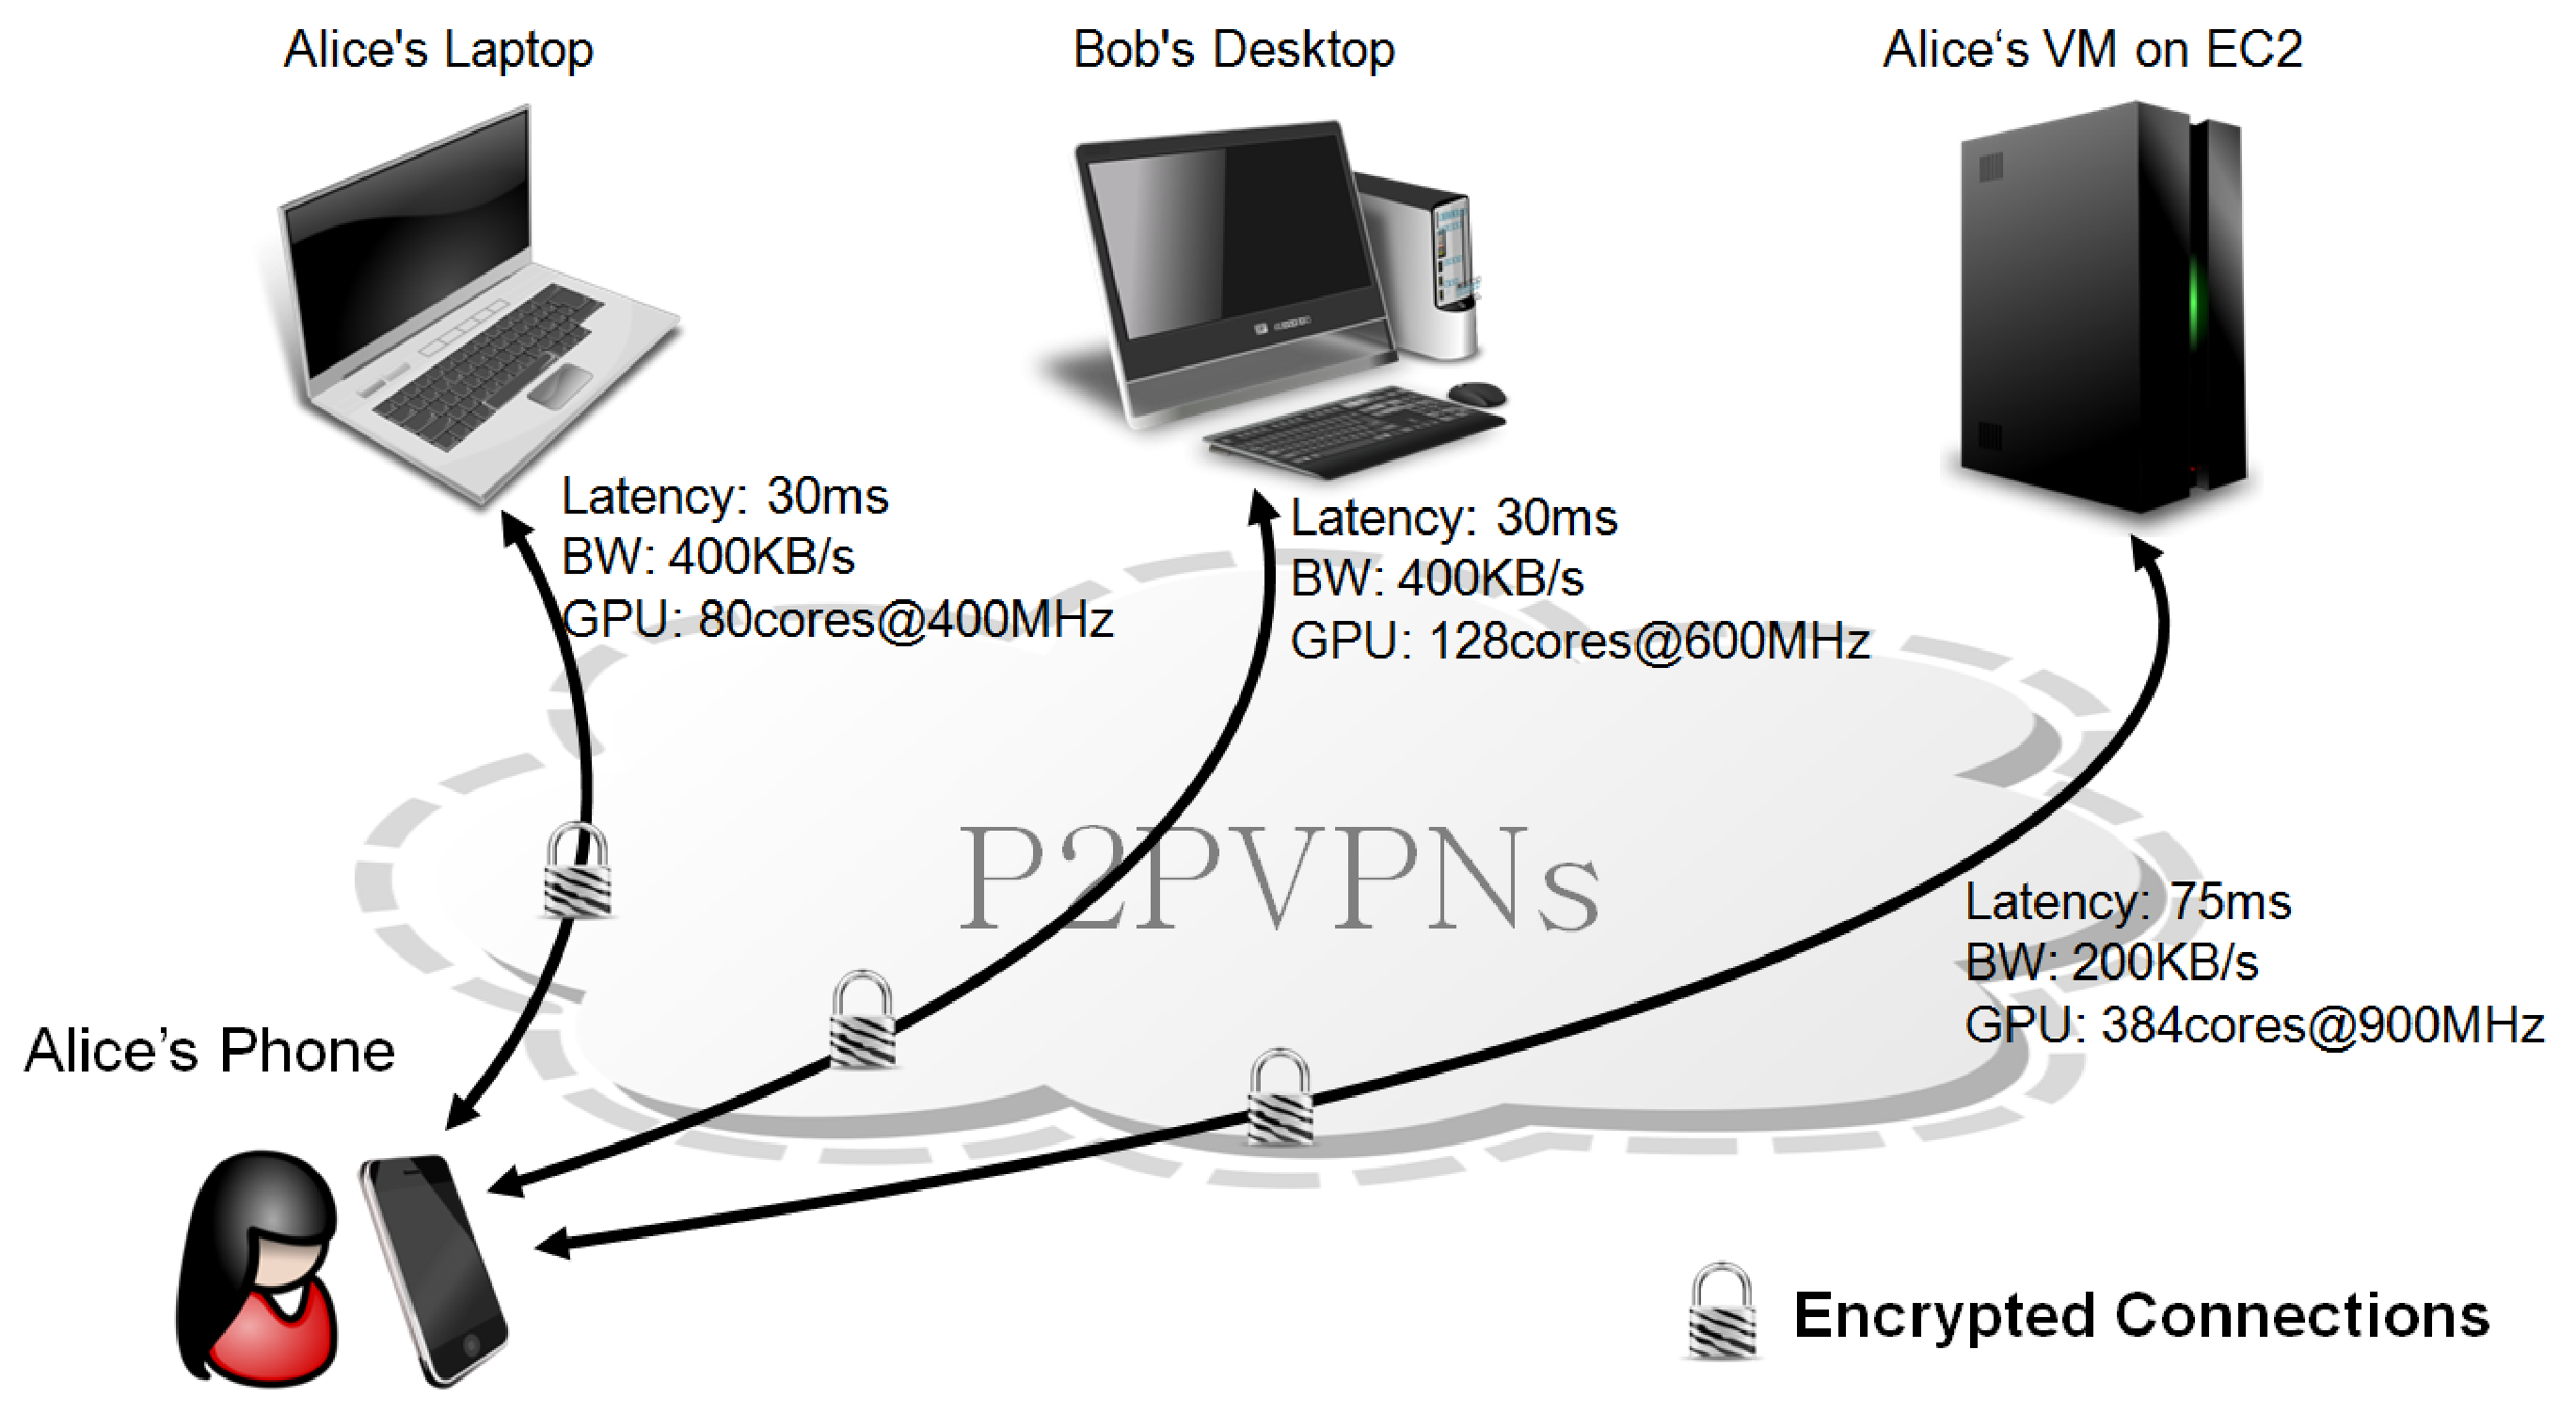
\epsfig{file=figs/motivation.eps, width=5.5in}
\caption{Private networking and node selection}
\label{fig:motivation}
\end{figure}
%
Here is another example of how a developer might take advantage of
OpenCL and the proposed platform in a seamless fashion.
%
Consider a typical facial recognition application in a mobile device
used as a security feature, or for tagging friends on a social
networking application.
%
First, the developer utilizes a CPU implementation.
%
However, the developer quickly realizes the processing limitations of
doing image processing on the CPU and decides that such a workload is
better suited for the GPU or another hardware-based accelerator.
%
With this realization, the developer writes an OpenCL-based
implementation due to its wide support and adoption.
%
Using OpenCL, the developer is able to offload the computation from the
mobile CPU to the mobile GPU and therefore achieve better performance
with less battery consumption.\\
%
The proposed framework aims to extend the umbrella of heterogeneous
computing to include devices beyond the physical host platform.
%
By recompiling the application to link with the proposed framework, the
developer can transparently access remote resources available via the
SocialVPN, including GPUs running on computing resources more powerful
than a mobile device.
%
For instance, if the mobile device is connected to a virtual network
consisting of an Amazon EC2 GPU instance, and the user's personal
workstation, the extensions to the OpenCL framework will automatically
select the best candidate based on available device capabilities, and
network conditions as the target compute node for remote execution.
%
Also, the use of SocialVPN, ensures that computation is offloaded
securely to socially trusted nodes.
%
This enhancement occurs transparently to the developer and the user
requiring only code recompilation. 
%

\section{Contributions}
\label{intro:contributions}
The key contributions of this dissertation can be summarized as
follows:\\
%
{\bf Novel framework for remote computation offloading.} The primary
contribution is a novel framework which addresses the challenge of
remote computation offloading to resources in the cloud the paradigm of
extended hardware-layer heterogeneous computing.
%
Heterogeneous computing uses specialized hardware accelerators to
increase computing throughput and performance.
%
The proposed framework combines the power of cloud offloading with the
flexibility of heterogeneous architecture which expands the dynamic
execution range of mobile platforms, which are typically restricted by
power constraints.\\
%
{\bf Decentralized resource discovery mechanism.} Second
contribution of this proposal is a distributed method of resource
management which handles service discovery, access control, and data
privacy.
%
Previous mobile offloading solutions have not investigated a service
discovery mechanism by assuming the availability of remote computing
resources with static endpoints.
%
The proposed framework advocates a dynamic approach where candidate
computing nodes are discovered at runtime while allowing for a more
flexible design.
%
By using IP multicast-based discovery, the proposed system periodically
locates computing nodes which are available within their social device
network.\\
%
{\bf Workloads characterization using computation to communication
ratio.} 
%
I characterize mobile workloads for the suitability of offloading from
the perspective of {\it Computation to Communication ratio} which is
calculated by the time for workloads to be executed locally divided by
the data transfer time for remote offloading.
%
Thus, in this work, computation to communication ratio for mobile
workloads is a comprehensive measurement which mirrors three dynamic
parameters such as the volume of computation of workloads, the amount of
data to be transferred, and the network conditions.\\
%
{\bf Machine learning-based runtime scheduler.} Prior studies have
primarily focused on core mechanisms for offloading.
%
However, adaptive scheduling in such system is important because
offloading effectiveness can be influenced by varying network
conditions, workload requirements, and load at the target device.
%
In this dissertation, a study on the feasibility of applying machine
learning techniques to address the adaptive scheduling problem in mobile
offloading framework is presented as a third contribution.
%
By taking the algorithm complexity and scheduling performance into
account, a few machine learning algorithms are selected to implement
on/offline runtime schedulers for mobile offloading framework.\\
%
The prototype implementation of the proposed framework is evaluated,
with regard to end-to-end application performance and energy consumption
in mobile devices, through a variety of network configurations
representing local and wide area network, and various levels of remote
computing capabilities such as typical CPUs, GPUs as well as Amazon EC2
instances.
%
\section{Outline}
\label{intro:outline}
The rest of the proposal is outlined as follows.
%
Chapter 2 provides the necessary background and context for this
proposal.
%
Chapter 3 presents the key idea of extending an OpenCL standard to
support remote offloading framework and integrating the OpenCL API with
RPC-based remote service.
%
Also, in Chapter 3, the decentralized resource discovery mechanism
through a peer-to-peer virtual private network is presented.
%
Chapter 4 characterizes mobile workloads the perspective of computation
to communication ratio.
%
Also, Chapter 5 explains machine learning techniques for a runtime
scheduler for remote offloading system.
%
Chapter 6 describes an online training mechanism for machine
learning-based mobile offloading scheduler.
%
Then, Chapter 7 introduces a proximity-aware clustering system which can
lead an additional performance improvement in conjunction with mobile
offloading framework.
%
Lastly, in Chapter 8, the dissertation is summarized and future work
is detailed.
%

\chapter{BACKGROUND}
\label{chap:background}
This proposal brings together various technologies synergetically thus
us to reuse various existing tools.
%
By combining a heterogeneous computing framework, virtual private
networking, and IP multicasting, I propose a solution that is based on
well accepted academic and industry standard.
%
In this section, I elaborate on some of these current standards and
their impact on the proposed design.
%
\section{Heterogeneous Computing}
\label{back:heterogeneous}
An increasing number of hardware platforms are incorporating
heterogeneity for both energy and performance improvement.
%
Therefore,  it has been seen that primary host CPU cores are assisted by
various computing units for specialized functions offloading.
%
These specialized accelerators are aimed at speeding up specific
portions of the application code and differ from the general purpose
processor architectures.
%
In this subsection, I explain some of the different types of
heterogeneous platforms available nowadays.\\
%
{\bf Heterogeneous multi-core CPU combinations.}
In this design, high performing CPU cores are integrated with low
performing energy efficient cores.
%
Currently, some mobile and server platforms employ this
architecture~\cite{atom}.
%
The goal is to match the application execution requirements to the
smallest available core that can achieve the execution within required
performance limitations with lowest energy consumption.
%
In other cases, one big processor is utilized for controlling the
scheduler of multiple smaller cores~\cite{nvidia}.
%
Previous works have suggested that this combination can reduce energy
consumption by 39\%~\cite{kumar}.\\
%
{\bf CPU-GPU combinations.}
These platforms aim to accelerate graphics performance by including
specialized hardware to execute graphics functions.
%
The Graphics Processor Units (GPUs) consist of multiple execution units
and local memory that can efficiently process data and task parallel
instruction streams at a very high throughput.
%
This architectural property also make GPUs good candidates for executing
non-graphical functions that can exploit the data and task parallelism
at a large scale leading to evolution of a rich General-Purpose
computing on Graphics Processing Units (GPGPU) based offloading
frameworks.\\
{\bf Hardware accelerators.}
Increasingly specialized hardware accelerators are being integrated on
different platforms to provide faster execution times for
domain-specific application bottleneck functions.
%
The accelerators range from fixed function units to customizable and
programmable hardware (e.g. FPGAs).
%
In conjunction with the processor cores, the specialized hardware
accelerators assist in making the targeted applications perform better
by taking care of the functions that use a majority of core cycles.
%
This model makes accelerator integration a natural choice for platforms
that target specific usages and/or operate under real-time and power
constraints.\\
%
{\bf Remote offloading.}
%One of the contribution in this dissertation is to extend the definition
%of heterogeneity to include a new kind of platform component -- the
%execution units on remote resources.
%
With the advent of mobile era, remote execution to remote resources has
been one of the most common solutions to achieve better application
performance.
%
Due to the compute, memory and power limitations on mobile devices, most
of the applications divide their execution between the portions of local
processing and remote execution handling much of the complex and heavy
task.\\
%
%The proposed architecture aims to extend this model by providing mobile
%applications with the flexibility of using remote resources through a
%well-defined framework, namely OpenCL.
%
In this dissertation, one of the contributions is to extend the scope
of heterogeneity to include a new kind of platform component -- the
compute units on remote devices located in the private or public clouds.
%
Therefore, the proposed multi-layer framework allows for application to
discovery, enumerate, and use the remote devices as if they were local
devices.
%
The framework has the advantage of not only speeding application
execution times and saving mobile device energy consumption but also
allows for the construction of a virtual dynamic platform with tight
integration of heterogeneous components both on and off the host
platform.
%
\section{OpenCL}
\label{back:opencl}
%
Currently, OpenCL (Open Compute Language) is the most well-known
framework for offloading tasks to different compute units within a
heterogeneous host platform.
%
This framework provides an APIs which make it possible for application
developers to dispatch kernels for execution.
%
It is supported by the top chip makers such as Intel, NVIDIA, AMD and
ARM Holdings.
%
At the moment, OpenCL is used in the scientific computing arena as means
to leverage GPUs for high-throughput computations.
%
I implement the proposed design as a subsystem of the OpenCL framework.
%
The extension makes it possible for the OpenCL framework to discover
accelerators located on remote resources across the network.
%
Once these remote OpenCL devices are discovered, the application
developers is able to use the same interface to transparently offload a
kernel as if it was a part of the local platform.
%
\section{Secure Offloading with P2PVPN}
\label{back:p2pvpn}
Previous works have not focused on dealing with the privacy implications
of offloading mobile computation to the cloud for remote execution.
%
One solution can be to use socket layer encryption such as SSL/TLS when
sending data to the cloud, but the encryption overhead has not been
studied in past research.
%
As privacy concerns in mobile devices grow, this dissertation
recognizes that a robust mechanism to ensure privacy is a fundamental
requirement.
%
To address the privacy issue, the proposed design integrates a social
peer-to-peer virtual private network (SocialVPN~\cite{socialvpn}).
%
SocialVPN automatically discovers social peers on the Internet and
creates a private network consisting solely of these trusted peers.
%
It also handles the cumbersome task of cryptographic key management in a
distributed fashion thus enabling a robust, secure communication layer
with no single point of failure.
%
By emulating a virtual LAN, peers have private IP addresses to each
other allowing them to freely communicate even if they are both behind
network address translators (NAT) and certain firewalls.
%
Hung et al.~\cite{hung} suggested using a centralized VPN to ensure data
privacy.
%
Centralized VPNs (e.g. OpenVPN, Cisco VPN, L2TP) typically function by
allowing the VPN client to connect to a VPN gateway, which forwards UP
requests to the internal private network on behalf of the clients.
%
This model does not guarantee any privacy between the gateway and the
destination machine because it does not provide end-to-end encryption.
%
This is exacerbated in a public cloud where you have different and
unknown organizations sharing the same private network.
%
This lack of IP level data privacy is a primary reason that many
organizations are hesitant to run their private workloads in the public
clouds\cite{brodkin}.
%
SocialVPN addresses this issue by enforcing encrypted end-to-end
communication.\\
%
The other important aspect of SocialVPN is that it gives the user
complete control over their virtual private network.
%
A user can create a virtual network consisting only of his/her own
personal computing devices.
%
For example, Alice can create a VPN consisting of only 4 nodes: her
mobile phone, her laptop, her workstation at the office, and a VM
instance running on Amazon EC2.
%
Alice can also expand the VPN to include her family members, and closest
friends or scale it down dynamically.
%
If Alice only trusts her own personal resources, she simply limits her
VPN to allow connectivity to her machines, and the framework will only
have private UP connectivity to her nodes thereby making them the only
candidates for remote offloading.
%
If she wants to access to more resources, she can allow private IP
access to nodes belonging to her trusted friends and family, hence
enabling the framework to utilize them  as compute endpoints.
%
The assumption here is that all of these nodes will be running SocialVPN
software stack along with an OpenCL RPC-service to support the remote
execution.
%
\section{IP Multicasting in Private Networks}
\label{back:ipmulticast}
The Internet protocol does support multicasting; however, routers
usually block multicast traffic; hence multicasting is widely used for
decentralized service discovery within private networks.
%
For example, most network printers support local network discovery
through well-known standards such as Bonjour~\cite{bonjour}, or
Universal Plug and Play (UPnP).
%
Hence, all modern operating systems as well as smart appliances (i.e.
TVs, NAS boxes) rely on these IP multicast-based services mechanisms to
discover and communicate with each other.
%
Through integration with SocialVPN, the proposed offloading framework is
able to reues these IP multicasting techniques as the foundation for the
service discovery system and allow it to span across wide area networks.
%
With this decentralized approach, it is no longer necessary to register
services in a centralized directory.
%
When the mobile device decides to offload some computation, it sends an
IP multicast query over the network, SocialVPN automatically handles
this packet and sends it to all trusted peers in the private network.
%
Eligible peers are therefore able to advertise themselves to the
requestor.
%
This enables dynamic service discovery without having to hardcoded
endpoints in configuration files or depend on a directory service.
%
IP multicast support in SocialVPN enables us to follow the same
decentralized services discovery techniques that are widely used in the
private networks for network printers, DNLA compatible devices (e.g. TVs)
and storage boxes.
%



\chapter{OFFLOADING FRAMEWORK}
\label{chap:offloading}
%
\section{Motivation}
\label{offloading:motivation}
%
Heterogeneity is now the norm in commodity computing systems where
platforms possess a mix of computing units such as CPUs, GPU, and other
specialized accelerators.
%
OpenCL has therefore emerged as the open standard for parallel programming
for these heterogeneous platforms.
%
By providing a common standard along with the necessary toolchain, OpenCL
enables a uniform framework to discover, program, and distribute parallel
workloads to the diverse set of compute units in the hardware.
%
Graphics processing units (GPUs), in particular, have reached the extended
coverage due to their rapidly expanding use in general purpose computing
(GPGPU) with parallel programming of the OpenCL standard.
%
For that reason, there have been efforts exploring the advantages of
parallelism from the OpenCL framework by offloading GPGPU workloads
within an HPC cluster environment~\cite{rcuda,vocl}.
%
The primary motivation for offloading within a cluster is for more efficient
utilization of resources by allowing multiple compute nodes to share the same
GPU for general purpose computing.
%
These researchers clearly demonstrate that OpenCL (and CUDA)-based
remote offloading is a viable option which saves power through more efficient
sharing of heterogeneous compute units over the network despite the
communication overheads.\\
%
In this work, I shift this motivation from the HPC cluster environment
to mobile platforms by considering a different perspective to this
expanding body of research by adapting the OpenCL offloading approach to
a mobile cloud computing scenario.
%
Since previous works focused mainly on offloading OpenCL workloads in
HPC cluster environments with high bandwidth and low latency between the
nodes, it was easy to realize and assess the advantages.
%
However, the advantages are not as clear in the mobile cloud computing
scenario where OpenCL workloads are sent over the wide area on
network links with much lower bandwidth and higher latencies than 
cluster environments.
%
Moreover, since workloads are traversing untrusted networks in the
wide-area, a layer of network encryption is necessary to ensure privacy
and some level of the trust of the results from the remote compute node.\\
%
This section presents an OpenCL-based remote offloading framework designed
specifically for mobile cloud computing where OpenCL workloads can be exported
from a mobile node (i.e. an Android device) to the cloud (i.e.
an Amazon EC2 instance with GPU access).
%
This remote offloading framework consists of the following components:
1) a customized RPC system with optimizations for network tasking and
data marshalling, 2) a service discovery mechanism which selects the 
compute node with the lowest latency, and 3) a virtual private networking 
layer which provides transparent network encryption without any modification 
at the application layer.
%
The proposed system is implemented as a wrapper library around the OpenCL API; thus
allowing transparent integration of the OpenCL API with our framework 
without any code modification.
%
The offloading framework also makes it possible for the developer to 
dynamically discover accelerators located on remote computing nodes 
(i.e. in the cloud), virtualize these accelerators as if they would be
regular accelerators located on-board the local mobile device, and then
seamlessly offload computation to the virtual accelerators.\\
%
An additional contribution of this work is a distributed method of resource management 
which handles service discovery, access control, and data privacy.
%
Past mobile offloading solutions have not investigated a service discovery 
mechanism and they assume the static availability of remote computing nodes 
with fixed endpoints.
%
Instead, this work advocates a dynamic approach where eligible compute nodes are 
discovered at runtime, allowing for a more flexible design. 
%
I achieved this by using IP multicast-based discovery so that the
system periodically locates compute nodes available within their
networks.\\
%
Furthermore, the proposed approach supports accessing resources beyond the local
private network, broadening the accessibility to trusted compute nodes
across the Internet and the cloud.
%
In fact, previous offloading research has focused on sending workloads only to 
resources within private local area networks where there is some guarantee 
that the data is contained within the network.
%
This is accomplished by utilizing a social peer-to-peer virtual 
private network, SocialVPN~\cite{socialvpn}.
%
The use of a peer-to-peer VPN with social features has several benefits.
%
First of all, by providing virtual private IP addresses only to social peers, 
the endpoints discovered through the VPN are deemed trustworthy by the user -– 
creating a Social Area Networks.
%
Secondly, the IP layer security ensures data privacy and frees us from 
having to handle the cumbersome tasks of cryptographic key management, and 
socket layer encryption.
%
Through SocialVPN, the state and functions (called kernels in OpenCL) 
necessary for remote execution are sent privately and the results are 
authenticated and verified at the virtual networking layer.\\
%

\section{The Structure of Remote Offloading Framework}
\label{offloading:structure}
%
The overall architecture of the proposed framework consists of 5 main
modules: integration with the OpenCL API, RPC-based offloading
mechanism, decentralized resource discovery feature, runtime scheduler,
and trusted and private IP communication layer.
%
\begin{figure}
\centering
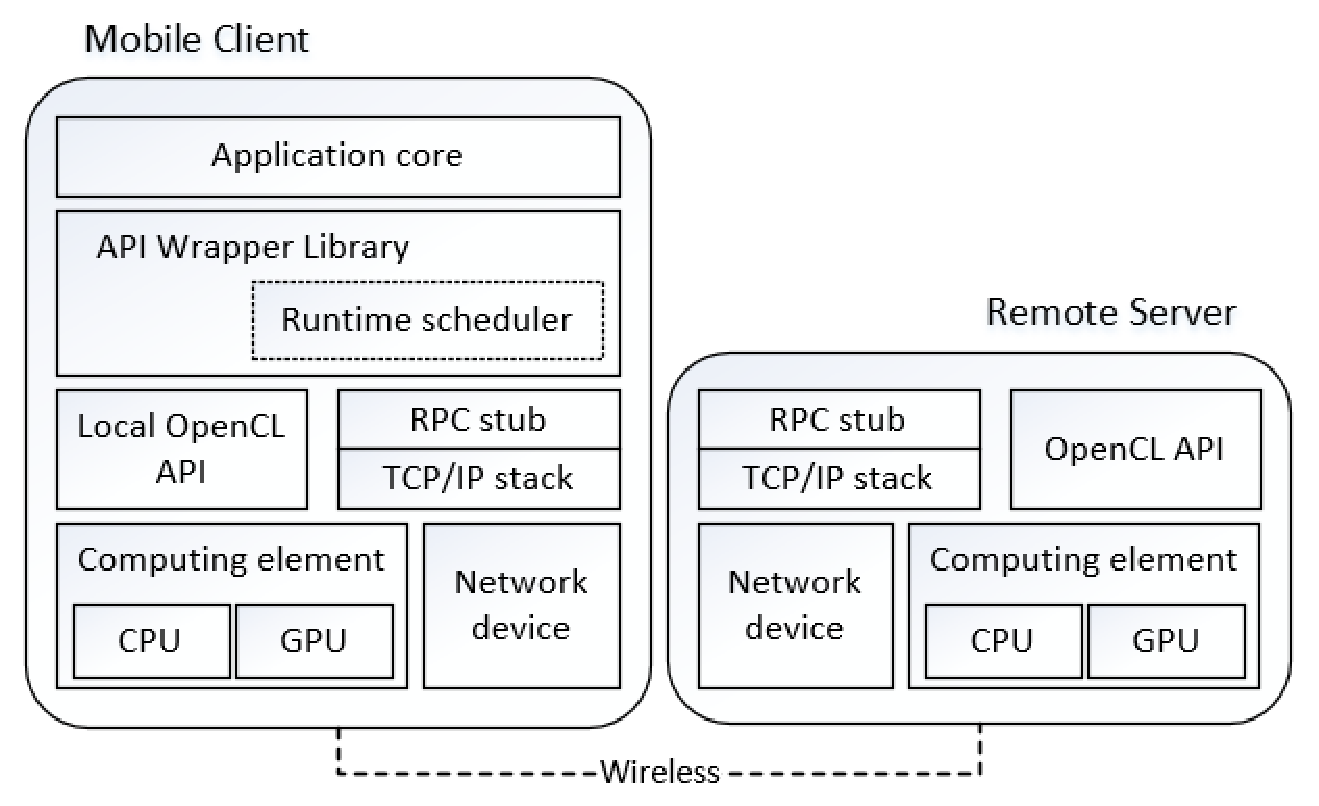
\epsfig{file=figs/overall_arch.eps, width=4.5in}
\caption{Overall system architecture}
\label{fig:architecture}
\end{figure}
%
\subsection{Transparent OpenCL API Extension}
\label{offloading:API}
%
Since OpenCL is an open standard currently supported by most of the
major device manufacturers, I chose not to deviate from their API in
order to minimize the learning curve for developers.
%
Latest revisions of the OpenCL specification are extending the coverage
to enable integration of a large pool of heterogeneous hardware under
the API.
%
Because OpenCL is also a hardware level offloading framework, it
provides various functions which can leverage in the proposed system.
%
The OpenCL API possesses a set of these features: device discovery and
enumeration, device selection and customization, buffer management,
job offload and status queries.
%
With these features, the application developer has a full control on the
use of specific accelerators necessary to optimize their application
performance.
%
In this section, I explain how these features can be extended to support
remote offloading framework.
%
Table~\ref{table:functionality} summaries OpenCL API functionalities and extensions.\\
%
{\bf Device discovery and enumeration.} In the initialization phase of the
interface, the developer queries the platform for on-board
OpenCL-capable accelerators.
%
The OpenCL framework returns a list of accessible compute devices
located on the board along with their computing capabilities (e.g.
graphics cards, video decoders, cryptographic devices).
%
In the case of a mobile device, this might include only a graphics
processor, or a specialized stream processor~\cite{stemcell}.
%
I extend this portion of the API by allowing the developer to discover
other OpenCL-enabled accelerators located on remote computing resources
over the network.
%
Hence, when the developer performs this type of the query on a mobile
device, it discovers not only the local mobile GPU but also another GPUs
running on the remote workstations or on the cloud, as long as they are
part of the same virtual private network.\\
%
{\bf Device selection and configuration.} In the standard OpenCL
framework, once presented with a list of devices, the developer selects
one or more targets for computation offloading.
%
This selection is usually based on the characteristics of each particular
device (e.g. the number of compute units of the accelerator, maximum
number of work items, architecture, latency or network bandwidth).
%
Based on the characteristics the developer is also able to configure the
workload appropriately for better performance.
%
Since this is a hardware layer offloading mechanism, the OpenCL framework
handles the support for different architectures by using a compiler
which converts the code from a modified version of C99 to the target
instruction set of the accelerator.
%
Hence, the API also provides access to compiler-based customizations for
both local and remote devices.
%
By extending the discovery process to include remote OpenCL devices over
the network, this selection and configuration process can become
cumbersome to the developer.
%
Thus, the proposed system can present only one virtual device handle
which represents the best offloading node according to network
conditions.\\
%
{\bf Workload state transfer.} Having selected a device, the next phase 
is the actual offloading of the data and code necessary to run workloads 
remotely.
%
The function to be executed (i.e. a kernel) is first sent either as C99 source
code or an LLVM-based intermediate language.
%
Once transferred, the code is compiled for the target accelerator.
%
In order to execute the kernel on the accelerator, the necessary state has
to be transferred to the device regardless of whether it is local or remote.
%
If the device resides on the host platform, the task of buffer management 
simply involves copying data from main memory to local storage accessible 
by the accelerator.
%
However, if the workload is being offloaded to a remote accelerator, then
the buffers have to be managed slightly differently.
%
First, the data has to be marshalled and copied into the buffers of the
networking stack, then transported over the network to the appropriate
remote host.
%
The data is then copied from the networking stack of the remote host
unto the accelerator's own local storage.
%
For example, in the case of a mobile device offloading computation to a
GPU hosted in the cloud, the necessary input and output buffers have to
be created and copied in the GPU's local memory in the cloud.
%
Upon completion, the output buffers are copied back from the GPU's local
memory to the mobile device's memory over the network.
%
Also, it is possible to perform data compression at the networking layer
to minimize the networking overhead and energy consumption.\\
%
{\bf Resource and failure management.} The final phase of the OpenCL API
is the ability to discover errors and release its state and resources in
a graceful manner.
%
Each function has its error parameter which keeps the developer aware of
the proper execution of the remote job.
%
If an error occurs due to an issue with the source code, the workload
configuration, or any other hardware issues, an appropriate error code
is returned to the developer.
%
In return, the developer can release the various resources (i.e. buffers,
device handles) that are associated with the job.
%
Once again, I extend this functionality to support network failures as
well.
%
In the case of a disconnection, the appropriate error code is returned
to the developer who then performs the necessary actions to clean up the
state belonging to the job.
%
On the server, the necessary clean-up is taken as well by the
framework.\\
%
The decision to utilize the OpenCL framework for computation offloading
in mobile devices allows us to leverage all of the functionalities
already in place for offloading computation locally from the CPU to an
on-board hardware accelerator.
%
I added the required extensions to the framework by creating a wrapper
library around the OpenCL API.
%
Since the offloading framework provides an identical interface,
developers can integrate their OpenCL code with the system without any
code modification. 
%
\begin{landscape}
%\begin{sidewaystable}
\begin{table}
	\centering
	\caption{OpenCL API functionalities and extensions}
	
	\begin{tabular}{p{3.0cm}|p{5.5cm}|p{3.5cm}|p{5.0cm}|p{3.7cm}} \hline
    \parbox{3.0cm}{\centering Feature} & \parbox{5.5cm}{\centering API
Function} & \parbox{3.5cm}{\centering OpenCL Feature} &
\parbox{5.0cm}{\centering Extension Capabilities} &
\parbox{3.7cm}{\centering Future Capabilities} \\ \hline

    \parbox{3.0cm}{\centering Discovery and \\Enumeration} & \parbox{5.5cm}{\centering \textit{} \\\textit{clGetPlatformIDs},\\\textit{clGetDeviceIDs},\\\textit{clGetDeviceInfo}
\\\textit{}} & \parbox{3.5cm}{\centering List on-board devices} &
\parbox{5.0cm}{\centering List the best remote resource} &
\parbox{3.7cm}{\centering List all remote resources} \\

    \parbox{3.0cm}{\centering Selection and \\Configuration} &
\parbox{5.5cm}{\centering \textit{}
\\\textit{clCreateContext},\\\textit{clBuildProgram},\\\textit{clCreateKernel},\\\textit{clSetKernelArgs},
\\\textit{clEnqueueNDRangeKernel} \\\textit{}} &
\parbox{3.5cm}{\centering Enables job compilation \\and configuration} &
\parbox{5.0cm}{\centering Configuration for the \\remote resource} &
\parbox{3.7cm}{\centering Configure \\multiple resources} \\

    \parbox{3.0cm}{\centering Workload \\State Transfer} & \parbox{5.5cm}{\centering \textit{}
\\\textit{clCreateProgramWithSource},\\\textit{clCreateBuffer},\\\textit{clEnqueueReadBuffer},\\\textit{clEnqueueWriteBuffer}
\\\textit{}} & \parbox{3.5cm}{\centering Source code and data transfer\\ over the
internal} & \parbox{5.0cm}{\centering Source code and data transfer\\ over
the network} & \parbox{3.7cm}{\centering Explore caching for\\ better performance} \\

    \parbox{3.0cm}{\centering Resource and \\Failure Management} &
\parbox{5.5cm}{\centering \textit{}
\\\textit{clWaitEvents},\\\textit{clFlush},\\\textit{clFinish},\\\textit{clReleaseBuffer},\\\textit{clReleaseProgram}
\\\textit{}}
& \parbox{3.5cm}{\centering Check on status and\\ cleanup} &
\parbox{5.0cm}{\centering Add support for network failure\\ and cleanup} &
\parbox{3.7cm}{\centering Enable timeout for\\ slow responses} \\ \hline
    \end{tabular}
\label{table:functionality}
%\end{sidewaystable}
\end{table}
\end{landscape}
%
\subsection{Integration of OpenCL API with RPC Service}
\label{offloading:rpc}
%
In order to support offloading on the remote resources, the offloading
framework utilizes an RPC-based service which handles offloading
requests received over the virtual private network.
%
As an first attempt, SunRPC service was utilized to provide the remote
procedure calling interface, serialization, and networking capabilities.
%
However, SunRPC provides many extra features that are not necessarily
efficient(for example, the use of a portmapper daemon to discover the
listening port of the RPC service).
%
SunRPC also initiates a new TCP connection for each function call which
incurs extra delay and the overhead on network performance.
%
In contrast, the proposed design uses a single TCP connection per
offloading job thus achieving lower latencies.
%
By running an RPC service which exposes the OpenCL API over the network,
the offloading framework provides a computation offloading design that
is lightweight in terms of argument serialization and buffer management.
%
Other approaches~\cite{vocl} rely on more sophisticated communication
primitives such as MPI which require extra processing and memory
resulting in poor battery performance.\\
%
\begin{figure}
\centering
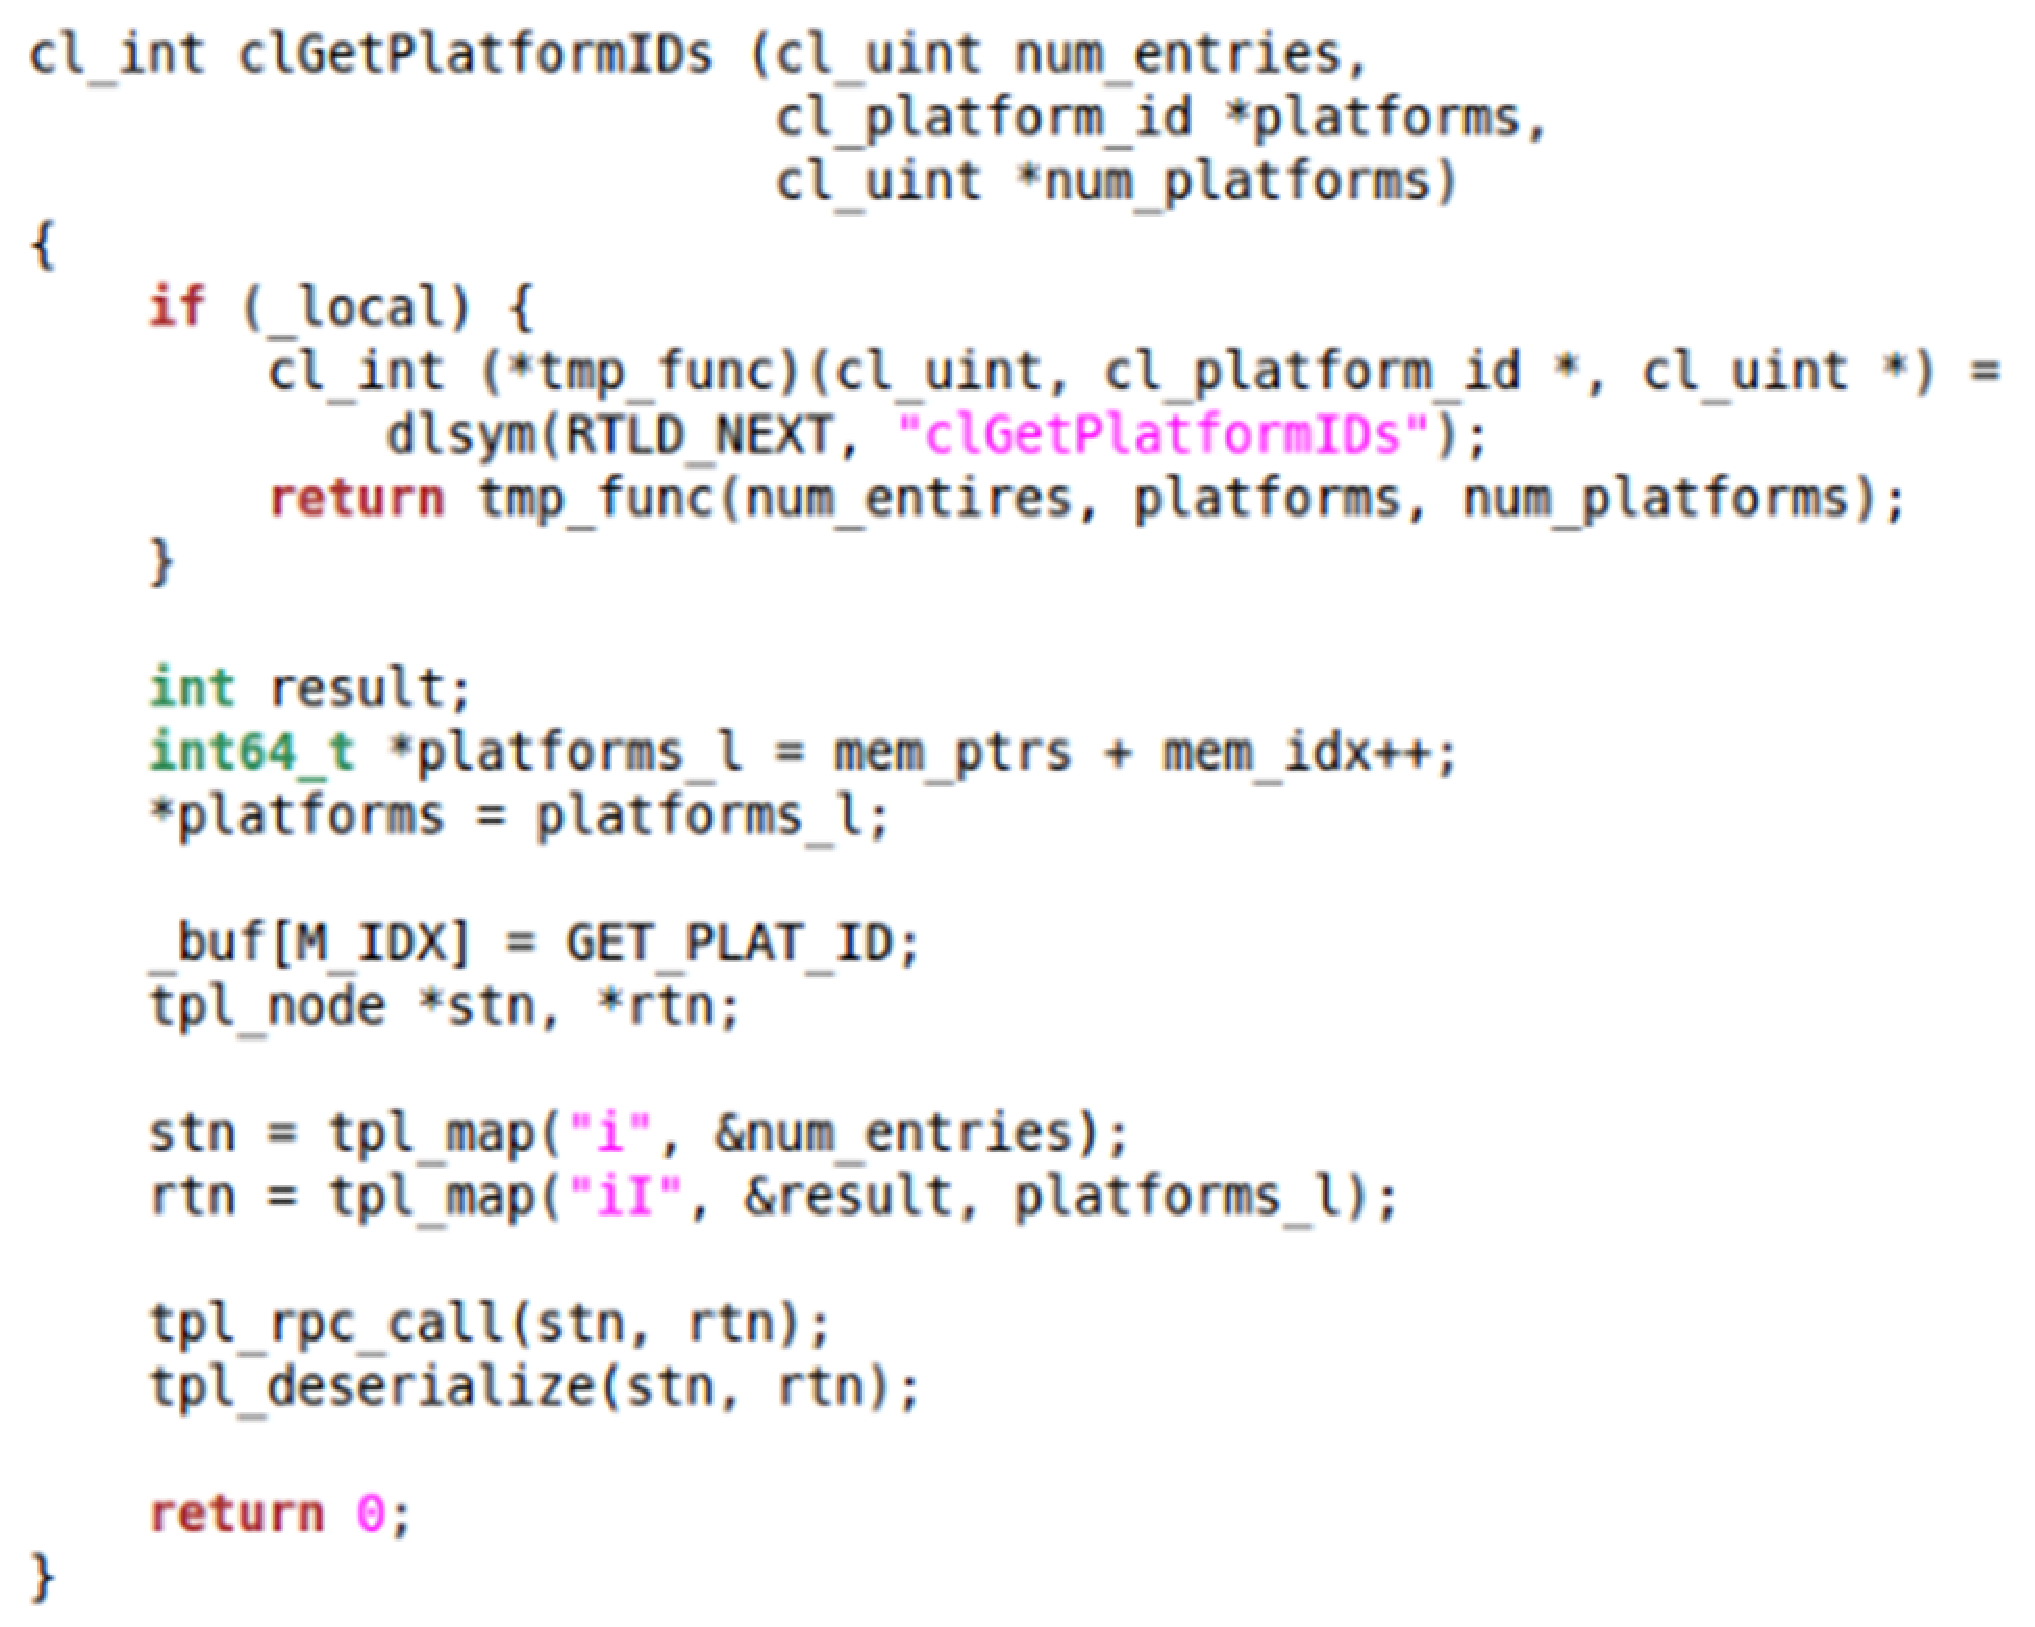
\epsfig{file=figs/code_rpc.eps, width=4.0in}
\caption{Code snippet for integration of OpenCL API with RPC}
\label{fig:code_rpc}
\end{figure}
%
The integration of OpenCL API with RPC-based service is realized as a
wrapper library which provides an identical interface to the original
OpenCL API.
%
Figure~\ref{fig:code_rpc} presents the codes snippet for wrapped
OpenCL API, {\it{clGetPlatformIDs}}, which is used to retrieve the
information of a targeted remote resource.
%
In the wrapper library, if a runtime scheduler, which will be described
in section~\ref{offloading:scheduler}, decides to execute the workload
locally, the wrapper library routes these API invocations to the original
local OpenCL library to invoke the corresponding OpenCL API.
%
On the other hand, the wrapper library serializes the API name and
arguments for remote execution, invokes the corresponding remote procedure
call, and sends them to the targeted remote resource over the network.
%
For data serialization, I use the efficient serialization package called
TPL data serialization~\cite{tpl}.
%
TPL can be used to serialize files, memory buffers and file descriptors
so that it is appropriate for use as a file format or inter-process
communication message format.
%

\subsection{Runtime Scheduler}
\label{offloading:scheduler}
%
As previously mentioned, the OpenCL-based remote offloading framework
provides developers with a list of accelerators(both local and remote)
to select as offloading targets.
%
However, some application developers may not want to bother with this
cumbersome task of figuring out which devices would make a good
candidate for local execution versus remote offloading.
%
The proposed framework provides a runtime scheduler which plays a key
role in the framework because it is the module that profiles performance
dynamically at runtime and codifies the policies designed to maximize
energy performance by selectively offloading tasks.\\ 
%
In the current implementation, the runtime scheduler consists of two
main parts: a resource profiler and a decision maker.
%
The default behavior of the resource profiler is to keep track of
network latencies to available remote resources and when the decision
maker requests the target to offload the workload, the profiler
provides the remote resource with lowest latency.
%
Then, the decision maker determines dynamically if the workload should
be offloaded or executed locally.
%
I  will explain the machine learning-based decision making in
section~\ref{chap:scheduler} in detail.\\
%
Currently, the resource profiler is an overly simplistic model by
considering only network latency as a feature for remote resource
selection.
%
Therefore, I plan on supporting a more complex set of conditions to
select the best remote resource.
%
For instance, by periodically recording the network
conditions (i.e. latency and bandwidth) measured at the VPN layer, and
others features such as computing capabilities of remote resources, the
profiler can automatically make the selection for which remote resources
would yield the best performance for a given condition while maximizing
a certain objective function on the utilization for remote resources.\\
%
This utility function-based resource profiler is motivated by my
previous research work on a peer-to-peer self-organizing and
self-managing cluster system based upon network coordinates and utility
function called SOLARE which stands for self-organizing latency-aware
resource ensemble~\cite{solare}. 
%
In the system, a peer-to-peer node periodically monitors the status of
the cluster in which it is currently involved, and whenever the utility
of the cluster is dropped below a threshold, it migrates to another
cluster to maximize the utility value.
%
In order to make use of utility function, I used two features: the
virtual distance to the cluster in artificial network coordinate system
and the number of current members in the cluster.\\
%
By adopting the module of utility function with different features for
utility function (i.e. latency, bandwidth, computing capabilities of
remote resources and so on), I expect that the remote resource profiler
provides more flexible ability of on-demand resource selection. 
%

\subsection{Decentralized Resource Discovery}
\label{offloading:discovery}
%
\begin{figure}
\centering
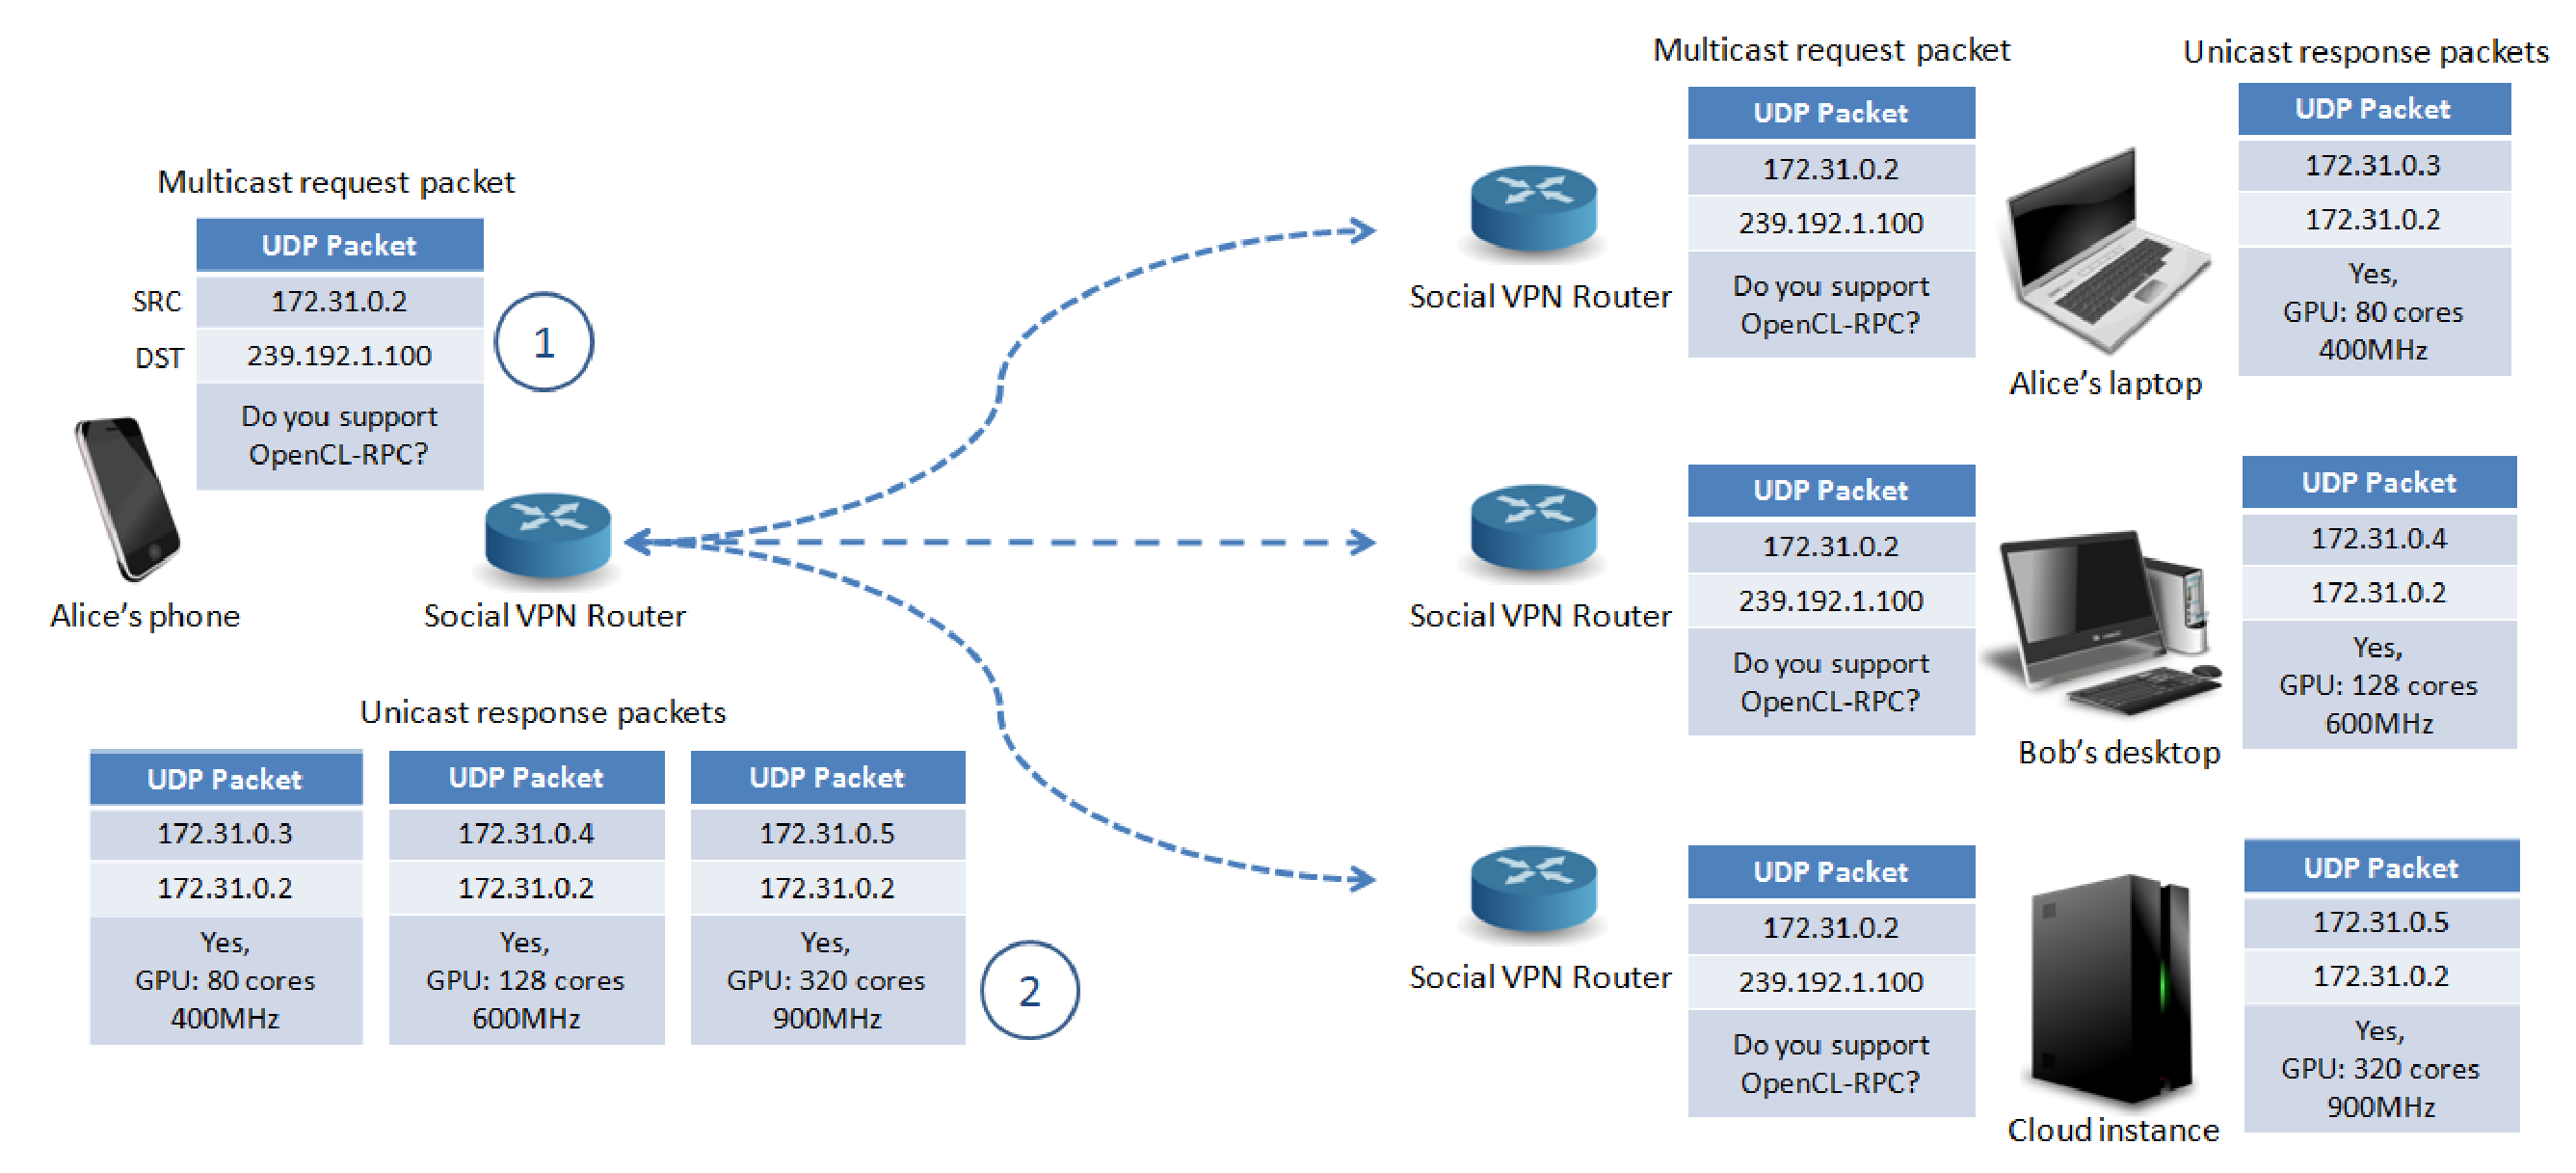
\epsfig{file=figs/discovery.eps, width=6.5in}
\caption{Decentralized resource discovery}
\label{fig:discovery}
\end{figure}
%
Current mobile offloading solutions rely on a centralized service to
provide the resource discovery capability.
%
A key differentiation of my approach is the decentralized IP
multicast-based remote resource discovery subsystem.
%
A challenge with IP multicast resource discovery mechanism is that the
vast majority of ISPs prevent multicast traffic from traversing their
network.
%
I sidestep this issue with network virtualization through SocialVPN.
%
Because the OpenCL-based remote offloading system is deployed on top of
SocialVPN which enables IP multicasting over the Internet, it is
possible to leverage existing LAN-based service discovery techniques for
wide area environment as well as local area environment.
%
The way that the decentralized remote resource discovery mechanism works
is illustrated in Figure~\ref{fig:discovery}.
%
The client periodically polls the network for eligible remote resources
by sending a UDP datagram to the multicast IP address.
%
The SocialVPN router distributes the IP packet to every remote resource
in the private network.
%
The RPC-based service described in section~\ref{offloading:rpc} has a
UDP listening thread that waits for resource discovery request and
responds to the request with its computing capabilities using the
requestor's unicast IP address.
%
The requester waits for a certain amount of time and accumulates all the
replies that it receives within that time window.
%
The requestor records their latency, bandwidth, and processing
capabilities and provides them to the scheduler.
%
The scheduler then determines which remote resource will provide the
best performance and selects that resource as the targeted candidate.
%
\subsection{Trusted Communication via VPN}
%
\label{offloading:vpn}
The virtual networking component addresses two key challenges of remote
workload offloading -- privacy and peer discovery -- while supporting
unmodified TCP/IP applications to offload computation to remote
computing resources.
%
In order to augment the mobile platform's computing capabilities, it is
important to find trusted resources that are not only in the same local
area network, but also geographically-dispersed peers, and to do so
dynamically an transparently to the mobile user's application.
%
While many VPN tunneling techniques would be applicable (e.g.
OpenVPN~\cite{openvpn}, Hamachi~\cite{hamachi}), the approach chosen in
the prototype is SocialVPN~\cite{socialvpn}, due to its ability to
autonomously create and manage VPN links to social peers, and its
support for tunneling IP multicast and discovery.
%
SocialVPN is a decentralized, self-configuring VPN based on online
social networking services such as XMPP and a public-key based security
model where certificates are exchanged and used to setup VPN links
automatically using online social network APIs.
%
SocialVPN ensures that friends anywhere on the Internet appear to be on
the same virtual LAN and end-to-end encrypted peer-to-peer tunnels are
abstracted as virtual IP links among friends.
%
SocialVPN  autonomously and continuously takes care of discovering and
exchanging public-key VPN certificates with social peers through online
social network infrastructures, handling the assignment and mapping of
virtual private IP addresses to devices, creating security associations
among peers, and capturing/routing IP packets for secure end-to-end
tunneling leveraging a peer-to-peer overlay.
%
By leveraging SocialVPN as a trusted peer-to-peer messaging substrate,
it is possible to use the Berkeley sockets networking interface to
offload the mobile workloads without any direct linking to SocialVPN
itself.
%
Most peer-to-peer systems require integration with a peer-to-peer
library as well as a learning curve for learning curve for learning its
API.
%
Because SocialVPN provides virtual private IP addresses to friends
instead of P2P addresses, it supports unmodified applications.
%

\section{Evaluation}
\label{offloading:evaluation}
%
In this section, I evaluate the implementation of the OpenCL-based
remote offloading framework for mobile platforms in terms of the
performance and energy consumption for mobile devices through real
deployment over local and wide area environments.
%
Firstly, I quantitatively analyze the overhead of the proposed resource
discovery mechanism in terms of energy consumption as a function of
number of remote resources.
%
Next, I will demonstrate the ability of the decentralized resource
discovery mechanism to dynamically discover remote resources under the
situation where the client offloads the workload iteratively to the best
resource with respect to the network latency while a few remote
resources occasionally join or leave the private network.
%
Also, I examine the overhead of adopting SocialVPN to the secure
communication between the client and the remote resource since SocialVPN
utilizes its own encryption and IP tunneling.
%
\subsection{Experimental Setup}
\label{offloading:setup}
In order to evaluate our remote offloading framework under a variety of
possible use case scenarios, I setup the experiments using various
hardware and network configurations.
%
First of all, for the mobile client, I utilized an Android table,
Samsung GalaxyTab 10.1 equipped with 1Ghz dual-core processor and 1GB
RAM, and running Android 3.1.
%
For the SocialVPN-connected remote resources, I utilized a workstation
with Intel 3.0Ghz Core2 Duo processor and 8GB memory installed with
Linux OS.
%
In addition, I used Amazon EC2 GPU cluster resource~\cite{amazonec2} and
FutureGrid virtual instances~\cite{futuregrid} for the remote resources which have
different computing capabilities and network performance.\\
%
For offloaded OpenCL workloads, I utilized OpenCL SDK code samples
provided by AMD SDK~\cite{amd} and NVIDIA~\cite{nvidia} such as
sobelfilter, matrix multiplication, N-body physics,
and hidden Markov model\footnote{I will describe more details about
OpenCL workloads that I chose for the experiments in
Section~\ref{chap:character}}.
%
Also, I emulate different wide area network conditions between the
client and the remote resource by controlling the network latency using
Traffic Control(TC)~\cite{tc}.
%
TC is a network tool which  provides functionality to control network
traffic by prioritizing network resources and using concepts of traffic
classification, queue disciplines and quality of service.
%
To profile energy consumption of the mobile device, I used
PowerTutor~\cite{powertutor} which is an application for the variants of
Android devices that displays the power consumed by major components
such as CPU, network interface, LCD display, and GPS receiver.
% 
\subsection{Overhead of Resource Discovery}
\label{offloading:overhead_discovery}
%
\begin{figure}
\centering
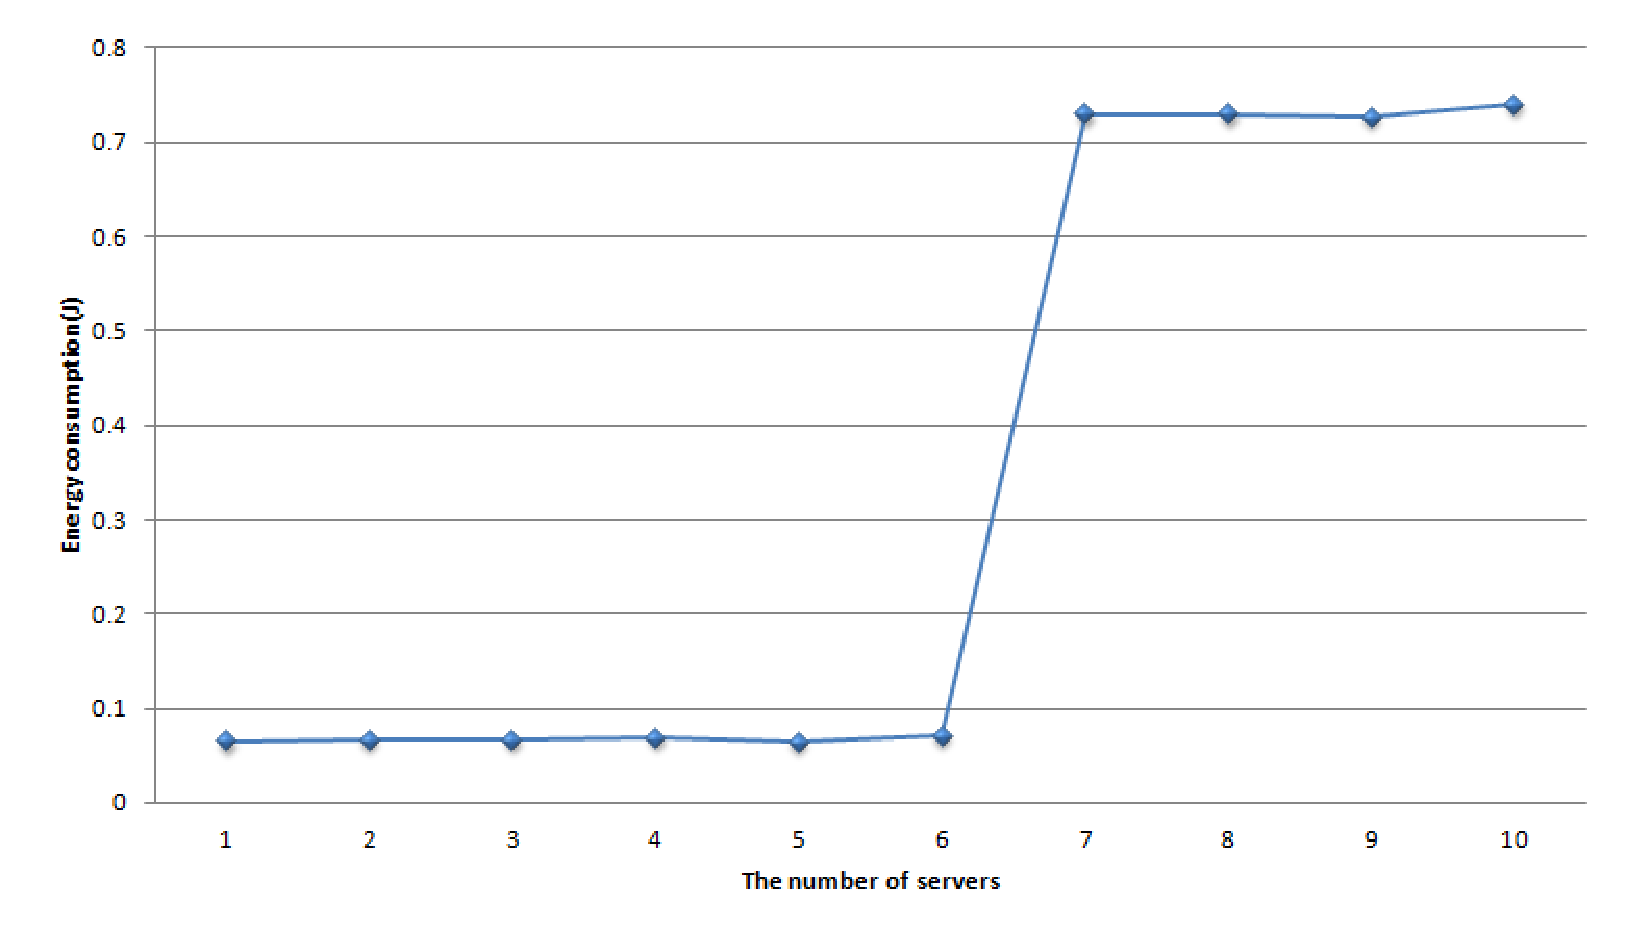
\epsfig{file=figs/energy_discovery.eps, width=4.5in}
\caption{Energy consumption for resource discovery mechanism}
\label{fig:energy_discovery}
\end{figure}
%
A novelty of this work is to allow the users to dynamically and
transparently discovery the remote resources through IP multicasting on
top of SocialVPN.
%
However, as the number of remote resources increases, the burden that
the mobile device has to handle also increases as well.
%
For that reason, it is essential to quantify the costs of the resource
discovery mechanism in terms of energy consumption of the mobile
devices.
%
I have conducted a WAN experiment in which 10 remote resources bound to
SocialVPN overlay are deployed in virtual machines at
FutureGrid~\cite{futuregrid} resources at University of Chicago,
University of California San Diego, and University of Texas, while a
client located at University of Florida requests the resource discovery.
%
Figure~\ref{fig:energy_discovery} shows energy consumption while the mobile
device performs the resource discovery for the given number of
resources.
%
As shown in Figure~\ref{fig:energy_discovery}, up to six resources,
energy consumption of the resource discovery does not vary
significantly, at less than 0.1J, regardless of the number of the
resources.
%
However, from seven resources onward, energy consumption jumps up to
0.7J.
%
This is because a typical WiFi networking device can tolerate the
number of packets to multicast resource request messages and to receive
the replies from up to six resources without entering into high power
mode.
%
However, the number of packets with seven resources crosses this
threshold pushing the WiFi device into high power mode and resulting in
more energy consumption.
%
It is worth noting that the overhead of energy consumption from resource
discovery mechanism depends on the interval of resource discovery which
means the trade-off between energy consumption and the accuracy of the
network characteristics of available remote resources.
%
In current setting, the resource discovery is repeated every 60 seconds
which means only 4.6\% of the overhead compared with when matrix
multiplication is executed locally consuming 15J of energy for 60
seconds(Section~\ref{character:energy}).
%
\subsection{Dynamic Resource Discovery}
\label{offloading:dynamic}
%
\begin{figure}
\centering
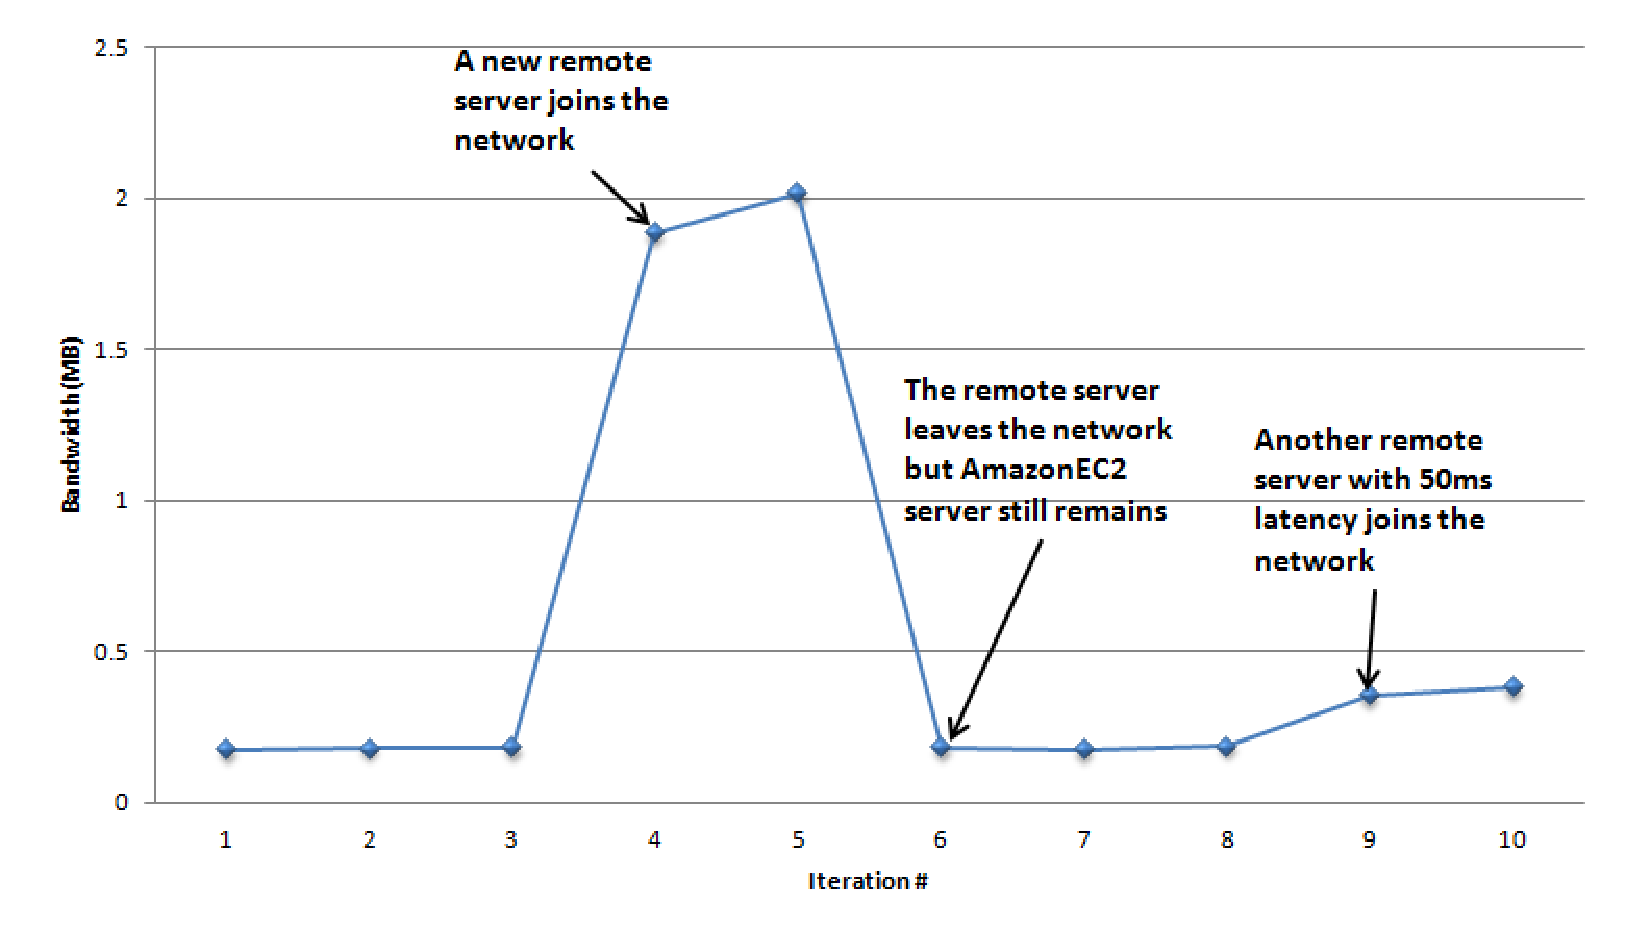
\epsfig{file=figs/dynamic_discovery1.eps, width=4.5in}
\caption{Bandwidth measurement}
\label{fig:dynamic_discovery1}
\end{figure}
%
\begin{figure}
\centering
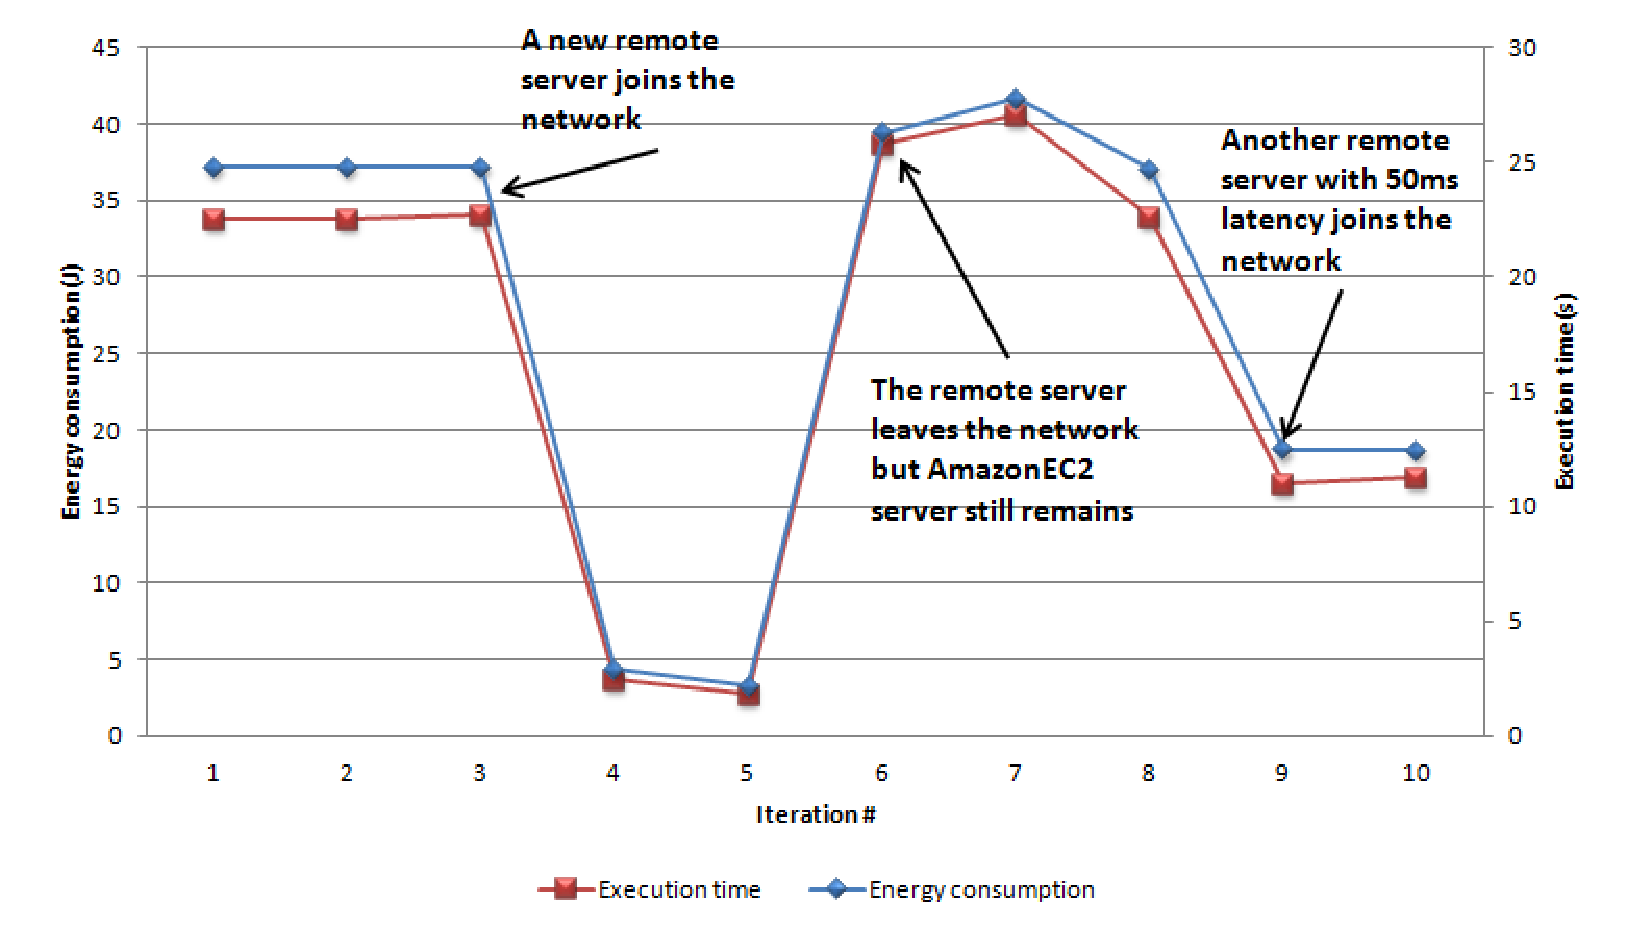
\epsfig{file=figs/dynamic_discovery2.eps, width=4.5in}
\caption{Performance measurement of remote offloading}
\label{fig:dynamic_discovery2}
\end{figure}
%
In this section, I demonstrate the ability to dynamically discover the
remote resources while the resources join or leave the networks and the
client offloads hidden Markov model to the remote resource.
%
For this, I designed a simple experiment in which the client offloads
the workload iteratively to the best resource with respect to the
network latency while a few servers occasionally join or leave the
network.\\
%
Firstly, when the client starts executing the workload, it has only one
available remote resource launched at Amazon EC2 GPU cluster and
offloads the workloads until a better remote resource is available.
%
At the fourth iteration, a new remote resource, which has less than 10ms
latency, joins the network.
%
As a result, the client connects to the new remote resource and switches
offloading to the new resource.
%
And then, at the sixth iteration, the remote server leaves the network
but Amazon EC2 resource still remains, so the client offloads the
workload to Amazon EC2 resource again.
%
Finally, another new remote resource with 50ms latency joins and the
client contacts to that resource.
%
Figure~\ref{fig:dynamic_discovery1} and ~\ref{fig:dynamic_discovery2} show the
available bandwidth to the best resource and the performance of remote
offloading respectively while resources join or leave the private
network.
%
\subsection{Overhead of SocialVPN}
\label{offloading:overhead_socialvpn}
%
\begin{figure}
\centering
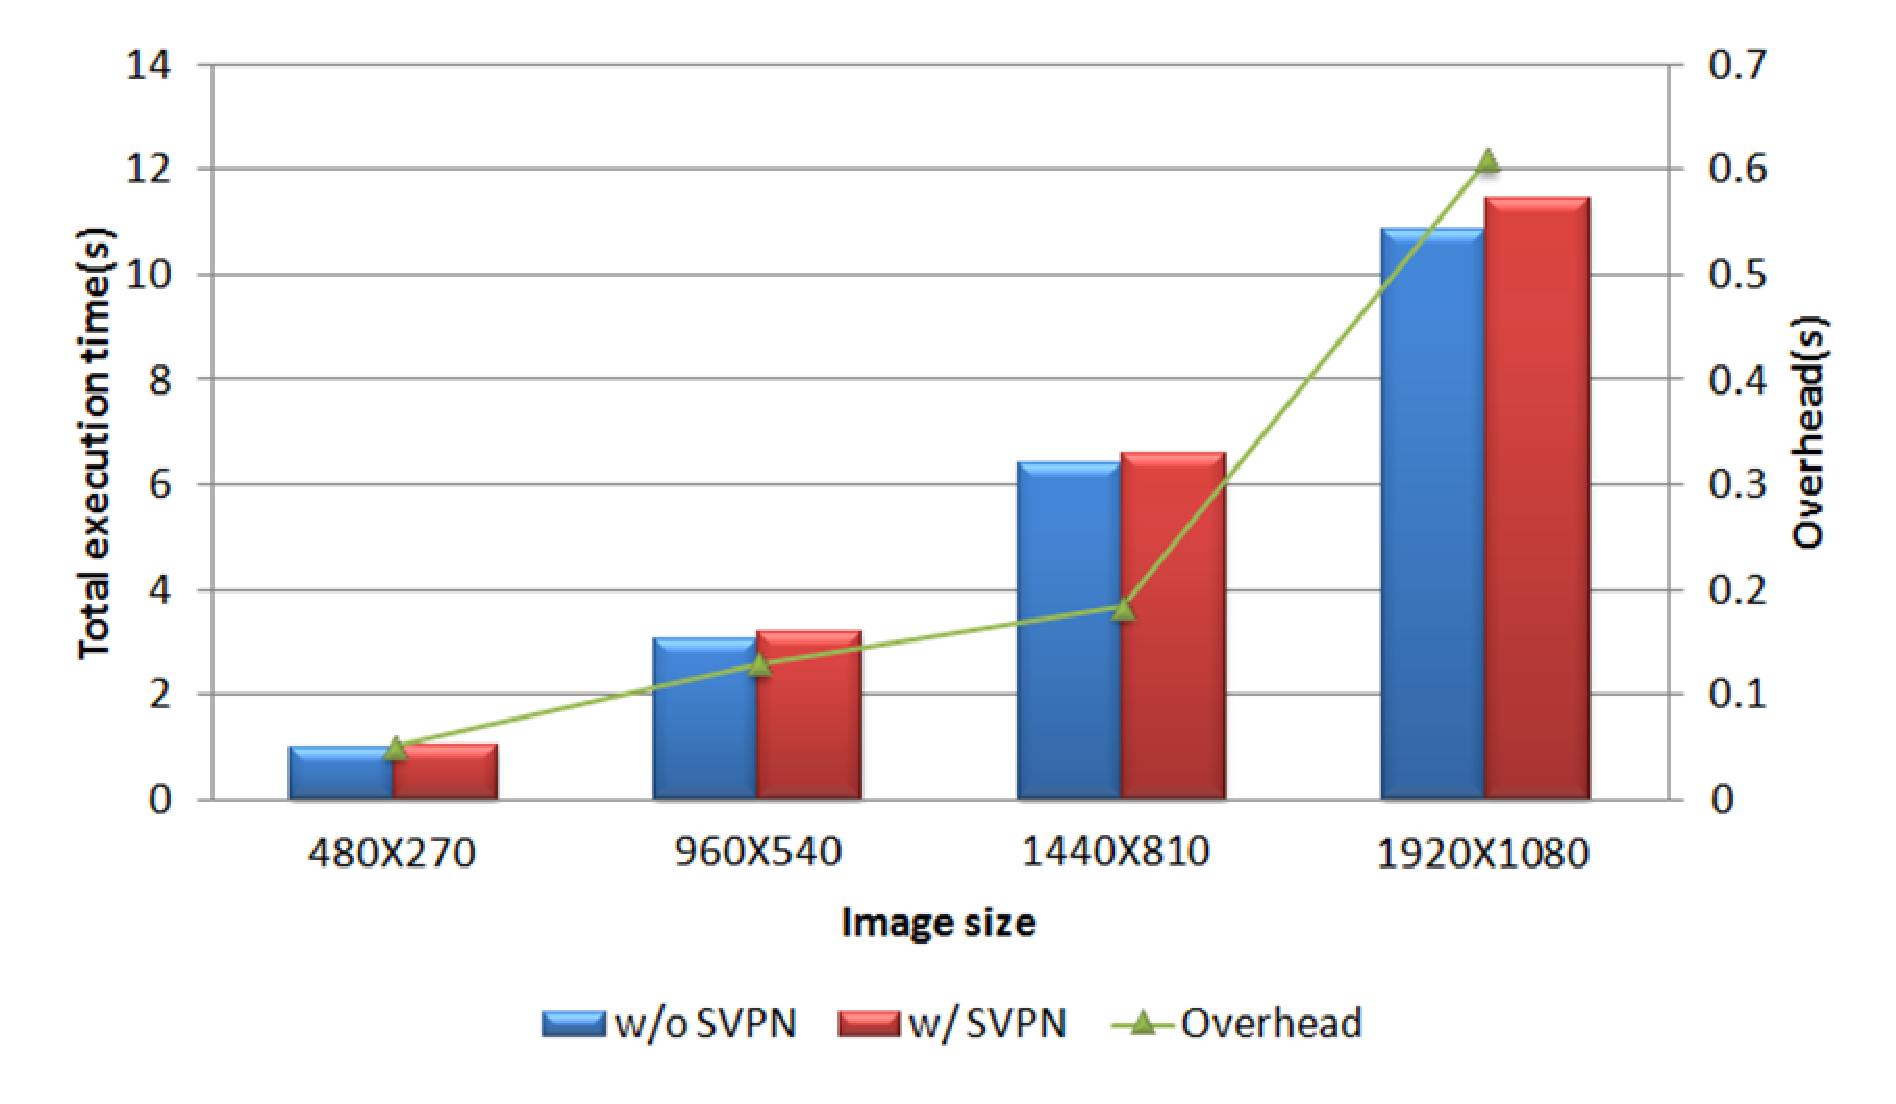
\epsfig{file=figs/overhead_socialvpn1.eps, width=4.5in}
\caption{Overhead of SocialVPN in terms of execution time}
\label{fig:overhead_socialvpn1}
\end{figure}
%
\begin{figure}
\centering
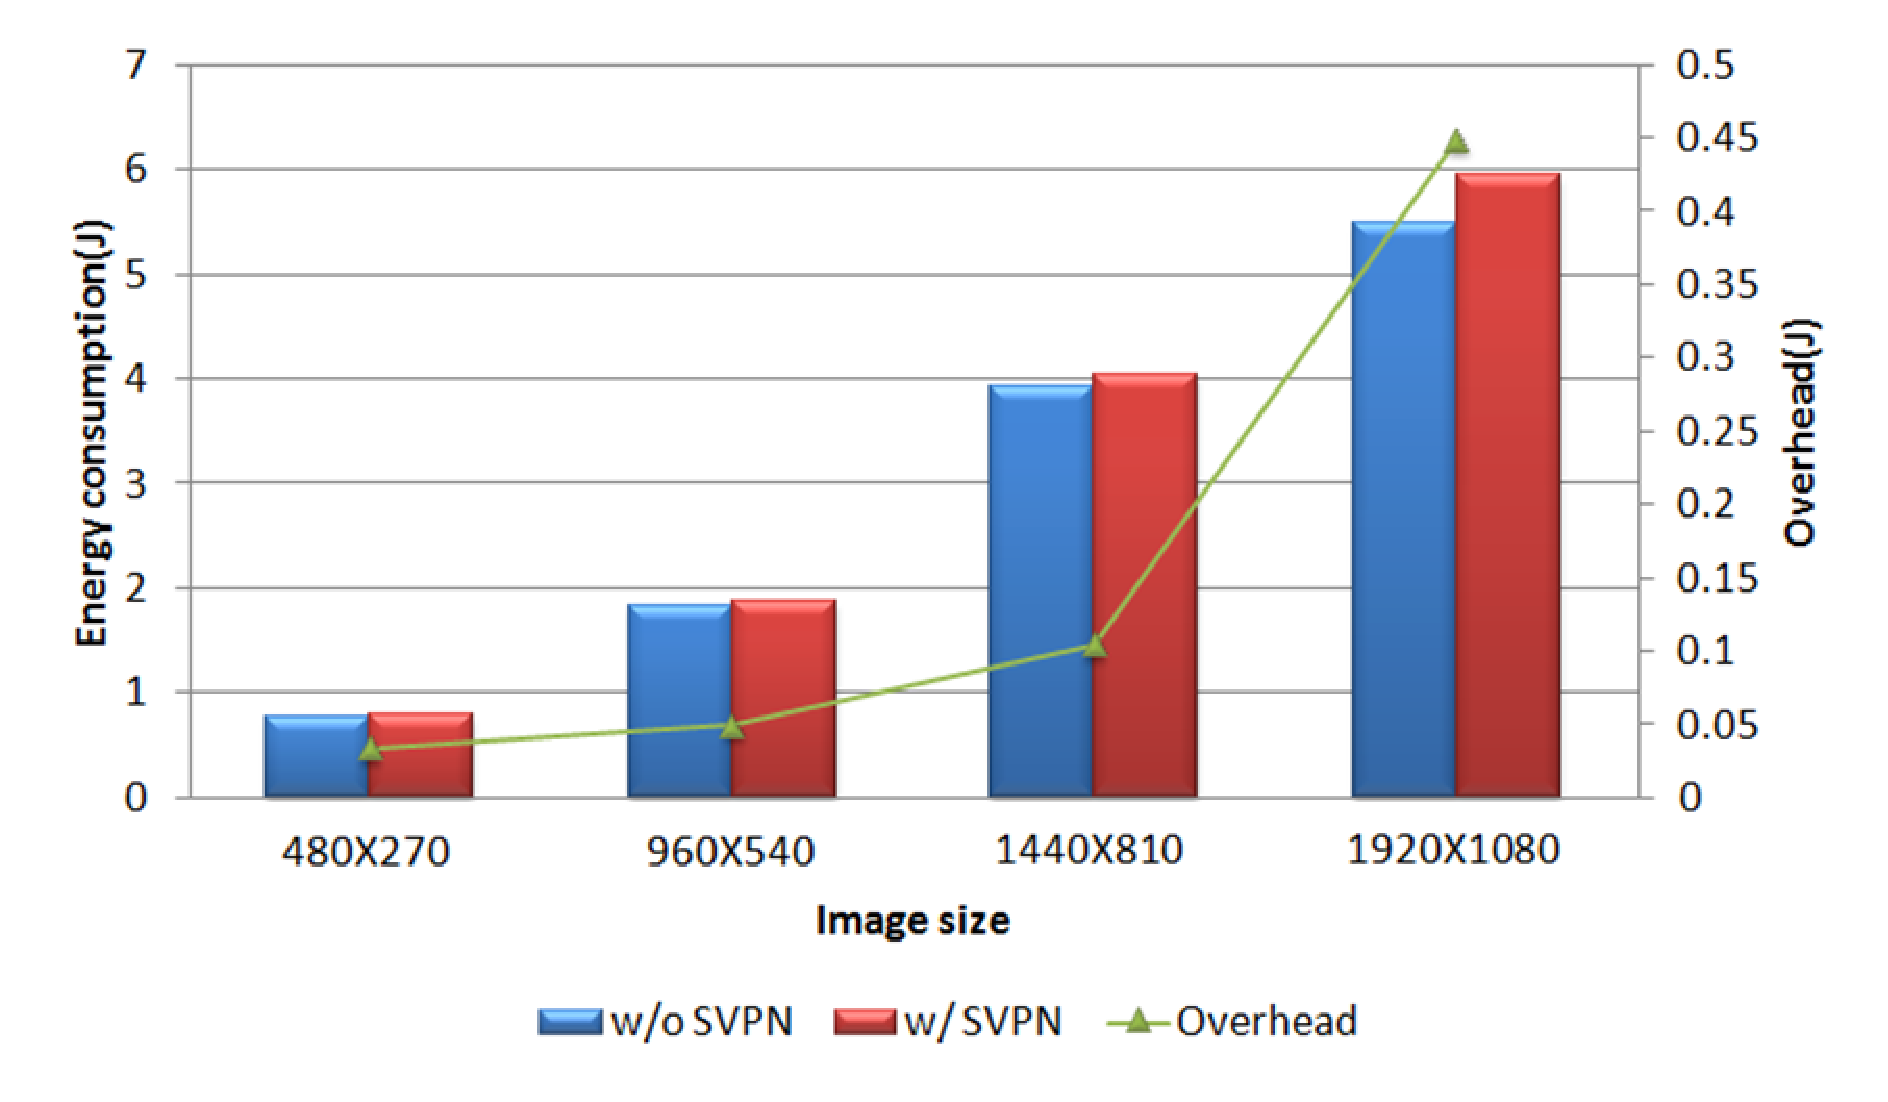
\epsfig{file=figs/overhead_socialvpn2.eps, width=4.5in}
\caption{Overhead of SocialVPN in terms of energy consumption}
\label{fig:overhead_socialvpn2}
\end{figure}
%
In the OpenCL-based remote offloading framework, SocialVPN enables
mobile devices and remote resources to securely communicate.
%
This incurs overheads due to encryption and tunneling.
%
In this section, I investigate the overhead of SocialVPN with respect to
the performance and energy consumption.
%
In order to measure the overhead of SocialVPN, I have conducted the
experiments in local area networks in which the client offloads OpenCL
workloads to the remote resource both with and without SocialVPN.
%
I do not consider the wide area network experiments for this comparison
because the resource discovery mechanism without SocialVPN is not viable
in wide area networks due to hindering of multicast by ISPs.\\
%
Figure~\ref{fig:overhead_socialvpn1} and ~\ref{fig:overhead_socialvpn2}
show the offloading execution time and energy consumption with and
without SocialVPN, respectively.
%
Even though I carried out the experiments using all of the workloads
I implemented, I only present the results from sobelfilter because
other workloads also show the similar trend as sobelfilter.
%
As shown in Figure~\ref{fig:overhead_socialvpn1}, as the image size
increases, the execution time and energy consumption also increase.
%
In the case of 480$\times$270 of image size, for instance, offloading with
SocialVPN takes 0.05s more than without SocialVPN while it takes 0.6s
more to offload 1920$\times$1080 of image size which means that the
overhead ranges from 2.8\% to 5.6\%.
%
In Figure~\ref{fig:overhead_socialvpn2}, I also observed the overhead
ranging from 2.6\% to 8.1\% in terms of energy consumption.
%
SocialVPN appends 80 bytes of an additional header to every packet to
tunnel regular TCP/IP packets where the default MTU(Maximum Transmission
Unit) for the experimental setup is 1,480 bytes.
%
For that reason, I approximately calculated about 6\% of the overhead
coming from SocialVPN.
%

\section{Summary} 
\label{offloading:summary}
In this section, I presented the OpenCL-based remote offloading
framework designed specifically for mobile cloud computing where OpenCL
workloads can be exported from a mobile device (i.e. an Android device)
to trusted remote resource (i.e. friend's desktop or family's laptop) or
even to the cloud resource (i.e. an Amazon EC2 instance with GPU
access).
%
The proposed remote offloading system consists of the following main
components: 1) a customized RPC-based service with optimizations for
network tasking and data marshalling, 2) a resource discovery mechanism
which selects the remote resource with the lowest latency, and 3) a
virtual private networking layer which provides transparent network
encryption without any modification at the application layer.\\
%
First of all, the prototype of the proposed remote offloading framework is implemented
as a wrapper library around the OpenCL API while allowing transparent
integration of the OpenCL API with RPC-based service without any code
modification.
%
Also, the IP multicast-based resource discovery mechanism makes it possible
for the mobile device to dynamically discover remote resources during
runtime and to utilize the computing capabilities of remote resources.
%
Furthermore, the proposed approach supports accessing resources beyond
the local private network, broadening the accessibility to trusted
remote resources across the Internet and the cloud.
%
This is accomplished by utilizing a social peer-to-peer virtual private
network, SocialVPN and creating a Social Area Network in which only
trusted social peers' computing resources are involved.\\
%
The evaluation showed that the use of SocialVPN resulted in a reasonably
acceptable overhead while guaranteeing secure connections and data
privacy.
%
Also, I demonstrated the ability to dynamically discover remote
resources while remote resources join or leave the network.
%
 

\chapter{WORKLOAD CHARACTERIZATION}
\label{chap:character}
%
In this section, I characterize mobile workloads for the
suitability of offloading from the perspective of {\it Computation to
Communication ratio} which is calculated by the time for workloads to be
executed locally divided by the data transfer time for the remote
offloading.
%
Thus in this work, computation to communication ratio for each workload is
a comprehensive measurement which mirrors three parameters such as the
volume of computation of workloads, the amount of data to be transferred, and the
network conditions. 
%
As part of the workload characterization effort through computation to
communication ratio, I strategically selected four quantitatively and qualitatively 
different OpcnCL workloads for the analysis:
sobelfilter, matrix multiplication, {\it N}-body physics and hidden
Markov model, each being classified into two categories: 
the computation-intensive workload (matrix multiplication and 
{\it N}-body physics) and the communication-intensive workload 
(sobelfilter and hidden Markov model) in terms of computation to communication ratio.
%
Note that though computation- or communication-intensity of
four OpenCL workloads is not absolute, it is worth to categorize 
the relative computation- or communication-intensity of the workloads so
it is possible to explore the workload conditions where offloading is
more beneficial than local processing.\\    
%
Furthermore, I deployed the offloading framework into the
various types of network such as local area networks, campus networks
and Amazon EC2 instance which have different network restrictions, and
set various levels of the computing capability of the remote
resource from general purpose CPUs to Amazon EC2 GPUs cluster instance to
analyze the behavior of the remote offloading framework in terms of the
performance and energy implication of mobile devices in accordance with
environmental factors such as network conditions and the computing
capabilities of offloadable resources.
%
For example, I configure local area networks by directly connecting a
mobile device and a remote resource with Nvidia graphics processing
units via a wireless router which represents the best resource of our
experimental setups.
%
The experimental results show that although not all types of workloads
benefit from mobile workload offloading, there clearly exist a class of
workloads and environmental conditions that can leverage the remote
offloading.
%
\section{Related Works}
\label{character:relatedworks}
In~\cite{fullsystem}, the authors characterize the microarchitectural
behavior of smartphone applications through several representative
benchmarks including the following areas: an interactive game, a
streaming player and mp3 audio player.
%
Also, they developed a new benchmark to characterize the performance 
of a web browser called BBench.
%
Through those benchmarks, they show how they differ from SPEC CPU2006
benchmarks which are widely used for the measurement of compute-intensive
performance.
%
MEVBench~\cite{mevbench} presented a custom benchmark suite for full mobile
vision applications such as augmented reality as well as components of
common vision algorithms such as SIFT feature extraction and SVM
classification.
%
The authors evaluated the performance of MEVBench with various
platforms for the direction of future mobile embedded vision
architectures.
%
Also, they show that mobile vision architectures require to be supported
from heterogeneous computation for performance improvement.
%
In~\cite{characterization}, the performance and energy benefits of
mobile heterogeneous computing are characterized by using 2D FFT(Fast
Fourier Transformation), matrix multiplication, and 2D Stencil as the
benchmarks.
%
In this study, the authors demonstrated that fully utilizing available
computing cores to complete a task can achieve an 3.7$\times$ speed-up
over the case of the single-threaded CPU, consequently, reduce the
energy consumption for the mobile platform.\\
%
In contrast with the aforementioned studies which designed new
benchmarks or characterized the performance and energy benefits of
the mobile platforms via the various workloads from a perspective of
mobile computing capabilities, I characterized the behavior of mobile
offloading framework while considering the network conditions as well as
the computing capabilities of remote resources.
%
\section{Methodology}
\label{character:methodology}
%
The main contribution of this work is to analyze the behavior of the
remote offloading in accordance with the characteristics of the
workloads and environmental factors such as network conditions and the
level of computing capabilities of remote resources.
%
In this section, I explain the workloads used for the analysis and the
way to characterize the workloads as well as experimental setup.
%
Every experiment is repeated 5 times and the results are the averaged 
values.
%
\subsection{Hardware Setup}
\label{character:setup}
%
In order to analyze the behavior of our remote offloading framework
under the various network conditions and the computing capabilities of
remote resources, I setup the experiment using various hardwares and
network configurations.
%
First of all, the hardware setup consists of a client and various types of
remote resources.
%
I have utilized Android tabletPC, Samsung GalaxyTab 10.1 equipped with
1GHz dual-core process and 1GB RAM, and running Android honeycomb as the
mobile client.
%
I adopted three types of servers: CPU only-installed server,
GPU-installed server, and Amazon EC2 GPU cluster.
%
For CPU only-installed server without a graphics card, I utilized a
workstation with Intel 3.0GHz Core 2 Duo processor and 8GB memory
installed with Linux OS.
%
Also, I installed GeForce GT 640 graphics card with 2GB RAM for the
server with GPUs.
%
In addition, I used Amazon EC2 GPU cluster resource with two Nvidia
GPUs equipped with 3GB on-board memory per GPU.\\
%
In order to analyze the impact of network conditions on offloading
performance, I configured both local and wide area networks using
following setup.
%
Firstly, I built a local area network by directly connecting the mobile
client and the server through a wireless router supporting 802.11 b/g/n
network standard.
%
Secondly, I used our campus network in order to configure a wide-area
network in which the client and the server connect to a wireless and
wired network respectively.
%
Also, I emulate different wide-area network conditions between the
client and the server by controlling the network latency using Traffic
Control (TC)~\cite{tc}.
%
TC is a network tool which provides functionalities to control network
traffic by prioritizing network resources and using concepts of traffic
classification, queue disciplines and quality of service(QoS).
%
Furthermore, utilizing an instance of Amazon EC2 GPU cluster gives us
one more option for the server located in wide-area network.
%
Table~\ref{table:network_summary} shows the average and standard deviation of network latency and
bandwidth for our network configurations.
%
\begin{table}
\centering
\caption{Average and standard deviation of network latency and bandwidth
for local and wide area networks including Amazon EC2.}
	\begin{tabular}{c|cc|cc|cc}
	\hline
	\ & \multicolumn{2}{c|}{LAN} & \multicolumn{2}{c|}{Campus network} &
\multicolumn{2}{c}{Amazon EC2} \\
	\hline
	Latency & Avg. & Stdev. & Avg. & Stdev. & Avg. & Stdev.\\
	(\textit{ms}) & 10.833 & 2.684 & 15.465 & 4.189 & 74.036 & 17.737 \\ 
	Bandwidth & Avg. & Stdev. & Avg. & Stdev. & Avg. & Stdev. \\
    (\textit{MB/s}) & 6.523 & 0.177 & 2.461 & 0.238 & 0.178 & 0.023 \\ \hline
	\end{tabular}
\label{table:network_summary}
\end{table}
%
\subsection{OpenCL Workloads}
\label{character:workloads}
%
I utilized OpenCL SDK code samples provided by AMD APP
SDK~\cite{amd} and Nvidia~\cite{nvidia} to choose appropriate workloads for
the remote offloading framework.
%
In order to choose appropriate OpenCL workloads among a set of samples,
I expected that the more computation- and less communication-intensive
the workloads, the more potential gain from remote offloading.
%
Furthermore, I characterized the workloads in accordance with the
amount of computation and communication for input and output data
transfer by considering computation to communication ratio
calculated by the execution time required to process a certain amount of
data locally divided by the data transfer time for the remote offloading.
%
Thus, computation to communication ratio is a
comprehensive measurement which mirrors three parameters such as the
the volume of computation of workloads, the amount of data to be transferred, and the
network conditions.
%
After careful considerations, I chose four qualitatively and
quantitatively different workloads: sobelfilter, matrix multiplication,
hidden Markov model, and {\it N}-body physics used by a variety of areas such as
image processing, physics simulation, and mathematical modeling.
%
Also, since it is necessary to consider an additional interaction 
between the client and the server such as device configuration 
or state transfer which occurs further overhead for communication, 
I examined the programming flow of the application-layer for each workload.
%
The programming flow and structure of workloads are described in the following:\\
%
{\bf Sobelfilter:} Sobelfilter is an image processing filter used for
image edge detection.
%
It consists of both a 3$\times$3 horizontal and vertical filter.
%
The edge detection process applies two filters into an input image in a
sequence and adds final results to a form of the image.
%
Accordingly, the client transfers the horizontal, vertical filter, and
the input image as states for the execution and sets them as arguments
accessed by the kernel.
%
In the server side, the image is iteratively processed based upon the
filters that the client has sent.
%
Once the execution is completed, the server sends back an output image
into the client.
%
Figure~\ref{fig:program_flow1} shows the program flow diagram for the data transfer, the argument
setup, and the kernel execution for sobelfilter.\\
%
{\bf Matrix multiplication:} Similarly to sobelfilter, the client
sends to floating-point matrices ({\it n} by {\it n} and
{\it n} by {\it 2n}) and additional small states and
arguments necessary for the remote kernel execution.
%
Then, server executes multiplication of two matrices and returns one
{\it n} by {\it 2n} matrix to the client as the result.
%
Therefore, matrix multiplication also follows the program flow of
Figure~\ref{fig:program_flow1}.\\
%
{\bf {\it N}-body physics:} {\it N}-body physics is a
mathematical simulation for predicting a dynamic system consisting of
particles or astronomical objects under physical forces such as gravity.
%
In the OpenCL workload for {\it N}-body physics, the client generates
initial states for a certain number of objects and sends them as an
input data.
%
However, the kernel takes additional arguments for each iteration of
kernel execution incurring additional communication between the client
and the server for the arguments setup.
%
The program flow for {\it N}-body physics is shown in
Figure~\ref{fig:program_flow2}.\\
%
{\bf Hidden Markov model:} Hidden Markov model is a popular
statistical tool for modeling generative sequences which can be
characterized by observable sequences.
%
It has been applied to a wide range of applications such as image,
speech recognition, computational biology, bioinformatics and
environment engineering.
%
The OpenCL workload for hidden Markov model follows similar steps for
kernel execution as \textit{N}-body physics.
%
The client generates and transfers initial states and transition
probabilities to the server.
%
Also, the client sends different arguments in order to execute each
iteration of the kernel.
%
Therefore, the program flow for hidden Markov model is represented by
Figure~\ref{fig:program_flow2}.
%
\begin{figure}
\centering
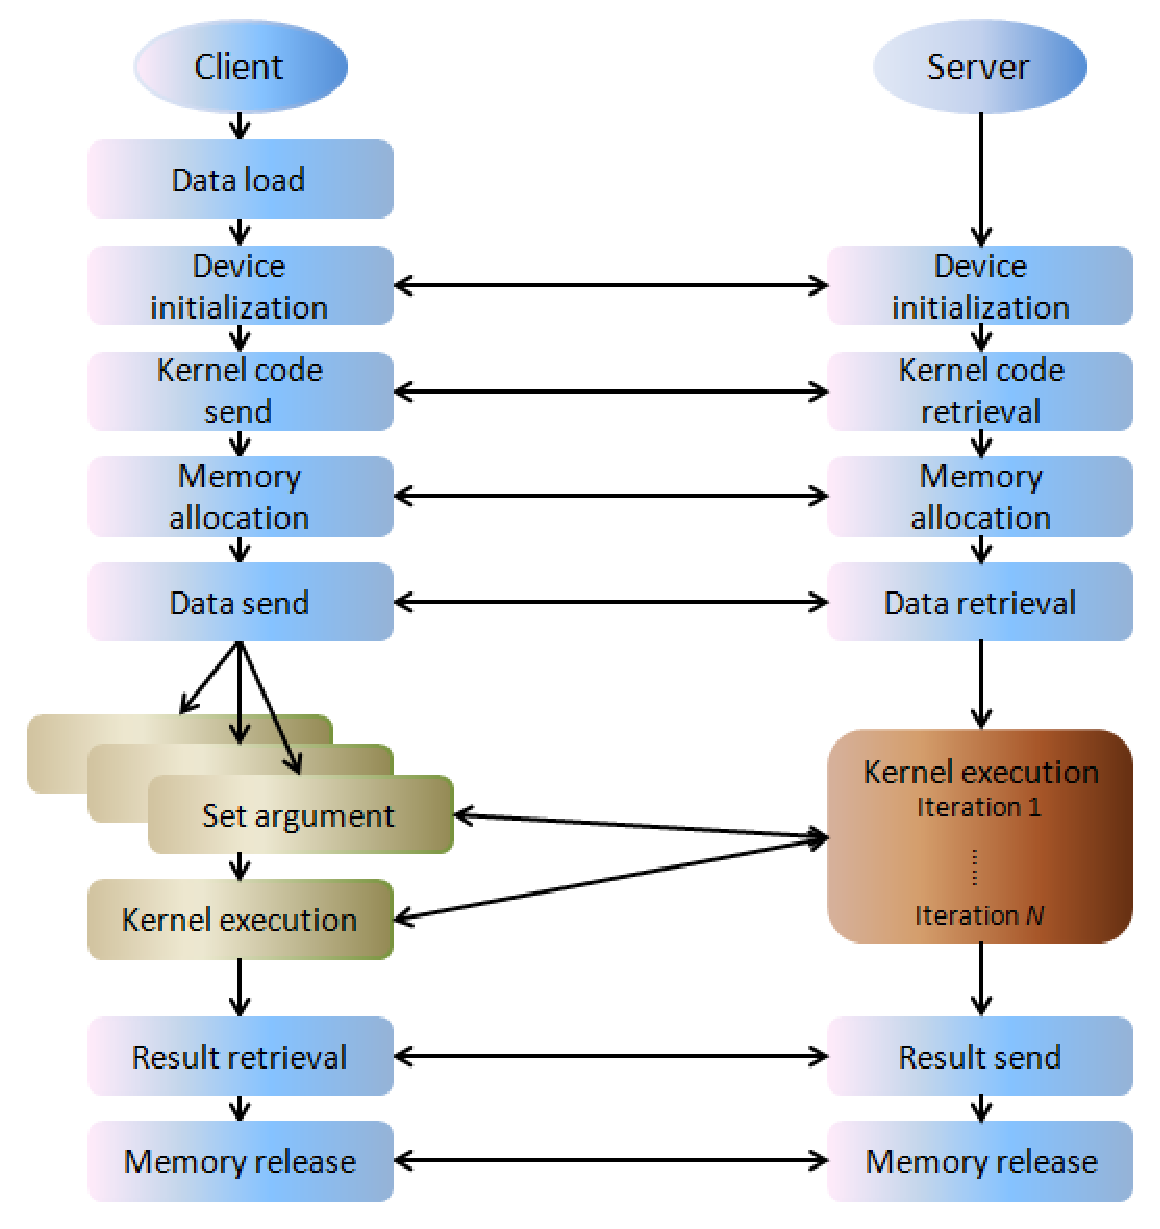
\epsfig{file=figs/program_flow1.eps, width=4.0in}
\caption{Program flow diagram for OpenCL workloads(A)}
\label{fig:program_flow1}
\end{figure}
%
\begin{figure}
\centering
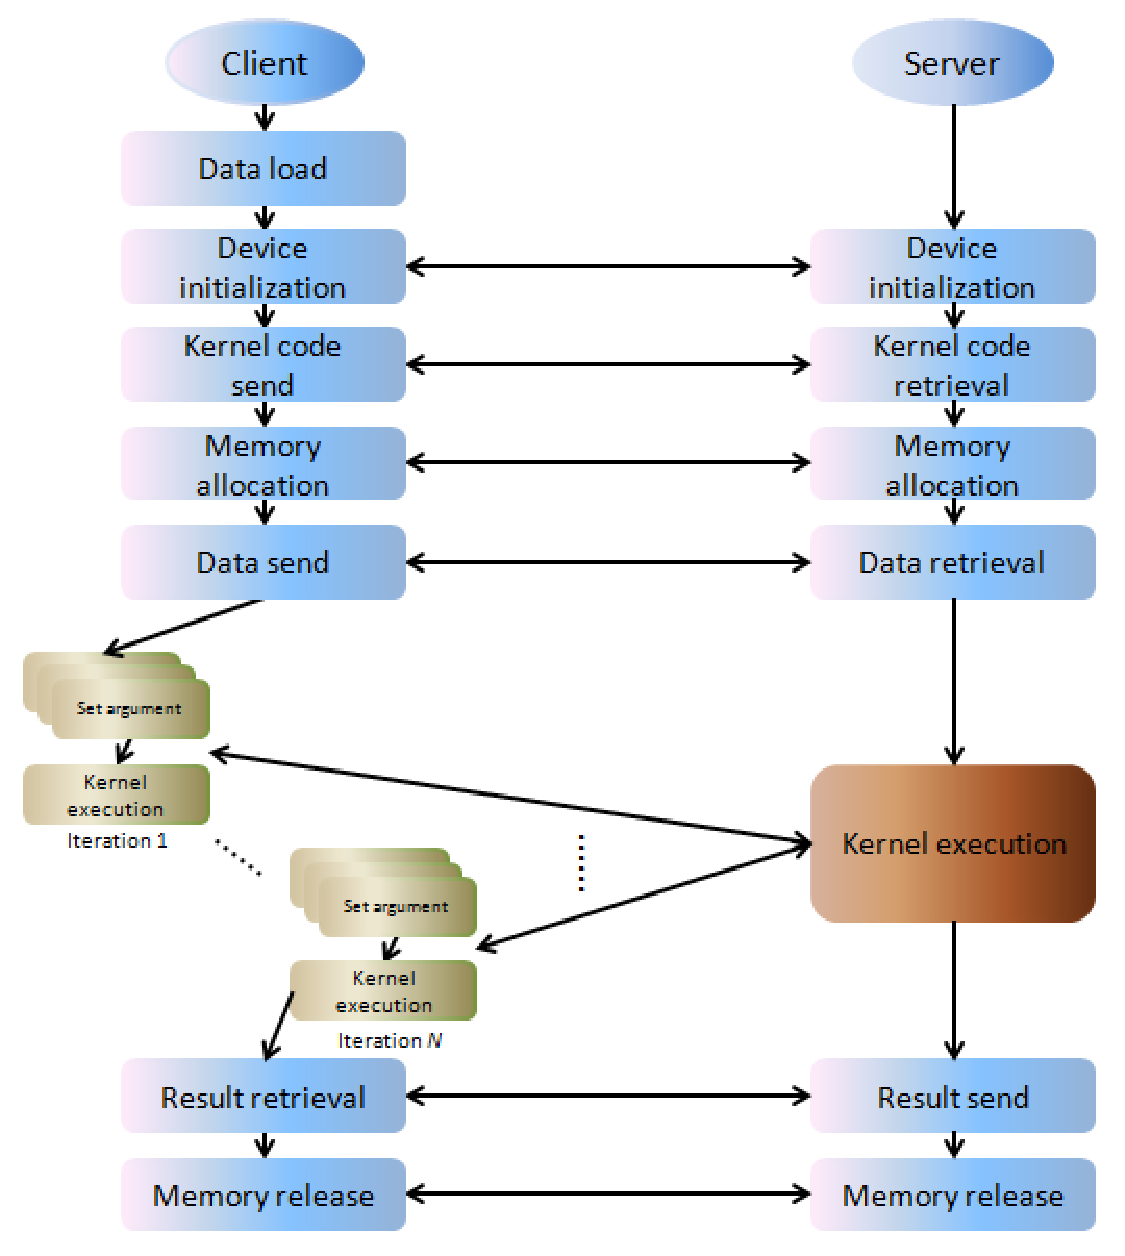
\epsfig{file=figs/program_flow2.eps, width=4.0in}
\caption{Program flow diagram for OpenCL workloads(B)}
\label{fig:program_flow2}
\end{figure}
%
\section{Analysis}
\label{character:analysis}
%
In this section, I analyze the behavior of the OpenCL-based remote
offloading framework for mobile platforms in accordance with the
workload characteristics and environmental factors such as network
conditions and the computing capabilities of remote resources through
real deployment over local and wide area environments.
%
First of all, I observe computation to communication ratios of the
workloads for the given size of data and network configurations.
%
Next, I evaluate the efficacy and the cost of the remote offloading
framework with the various network configurations and the remote
resources.
%
Table~\ref{table:workload_summary_sm} and~\ref{table:workload_summary_hn} 
summarize the amount of input and output data transfer, and the number
of additional API calls for argument setup required to execute the
OpenCL kernel code for the given size of data or the number of
iterations.
%
\begin{landscape}
%\begin{sidewaystable}
\begin{table}
\centering
\caption{Summary of input, output, and number of API calls for
sobelfilter and matrix multiplication}
	\begin{tabular}{c|c|c|c|c|c|c|c|c|c}
	\hline
	 \multicolumn{5}{c|}{Sobelfilter} & \multicolumn{5}{c}{Matrix
multiplication} \\ \hline
	Image size & 480$\times$270 & 960$\times$540 & 1440$\times$810 &
1920$\times$1080 & Matrix size & 160$\times$320 & 400$\times$800 & 560
$\times$1120 & 720$\times$1440 \\
	Input & 390 & 1,520 & 3,310 & 5,790 & Input & 270 & 1,720 & 3,390 & 4,610 \\
	Output & 110 & 370 & 720 & 1,190 & Output & 170 & 1,280 & 2,010 & 3,340 \\
	\# of API calls & 7(0.5) & 7(0.5) & 7(0.5) & 7(0.5) & \# of API calls & 8(0.05) & 8(0.05) & 8(0.05) & 8(0.05) \\ \hline
\end{tabular}
\label{table:workload_summary_sm}
%\end{sidewaystable}
\end{table}
\end{landscape}
%
\begin{landscape}
%\begin{sidewaystable}
\begin{table}
\centering
\caption{Summary of input, output, and number of API calls for
hidden Markov model and N-body physics}
	\begin{tabular}{c|c|c|c|c|c|c|c|c|c}
	\hline
	 \multicolumn{5}{c|}{Hidden Markov model} &
\multicolumn{5}{c}{\textit{N}-body physics} \\ \hline
	number of states & 288 & 640 & 928 & 1,216 & number of iterations &
5 & 10 & 50 & 100 \\ \hline
	Input & 290 & 1,470 & 3,200 & 5,500 & Input & 15 & 15 & 15 & 15 \\
\hline
	Output & 78 & 108 & 110 & 119 & Output & 30 & 30 & 30 & 30 \\ \hline
	\# of API calls & 1000(66) & 1000(66) & 1000(66) & 1000(66) &
\# of API calls & 20(0.16) & 40(0.32) &
200(1.6) & 400(3.2) \\ \hline
\end{tabular}
\label{table:workload_summary_hn}
%\end{sidewaystable}
\end{table}
\end{landscape}
%
\subsection{Computation to Communication Ratio}
\label{character:ctoc}
%
In this section, I present computation to communication ratio 
for each workload for the given size of data and network configurations.
%
As I expected, it is evident that for all workloads, computation to communication
ratio with local area networks is higher than other network
configurations, since the data transfer time becomes shorter by higher
network bandwidth from local area networks.
%
On the contrary to local area networks, the cases of Amazon EC2 have the
lowest computation to communication ratio because of its most restricted
network conditions.
%
As shown in Figure~\ref{fig:ctoc_sobelfilter} and~\ref{fig:ctoc_hmm}, however, 
computation to communication ratios 
for sobelfilter and hidden Markov model are relatively uniform
regardless of the size of data, while those for matrix multiplication
and {\it N}-body physics increase as the size of data or the
number of iterations increases. 
%
This is because that the volume of computation for sobelfilter and
hidden Markov model is linearly proportional to the amount of data to be
processed, while that for matrix multiplication and
{\it N}-body physics increases exponentially as the size of data or
the number of iteration increases, which means that the benefits from
offloading such workloads to more powerful resources also increase exponentially.
%
Therefore, I expect it is highly likely that more gain is available
from offloading matrix multiplication and \textit{N}-body physics 
as the size of data increases. 
%
\begin{figure}
\centering
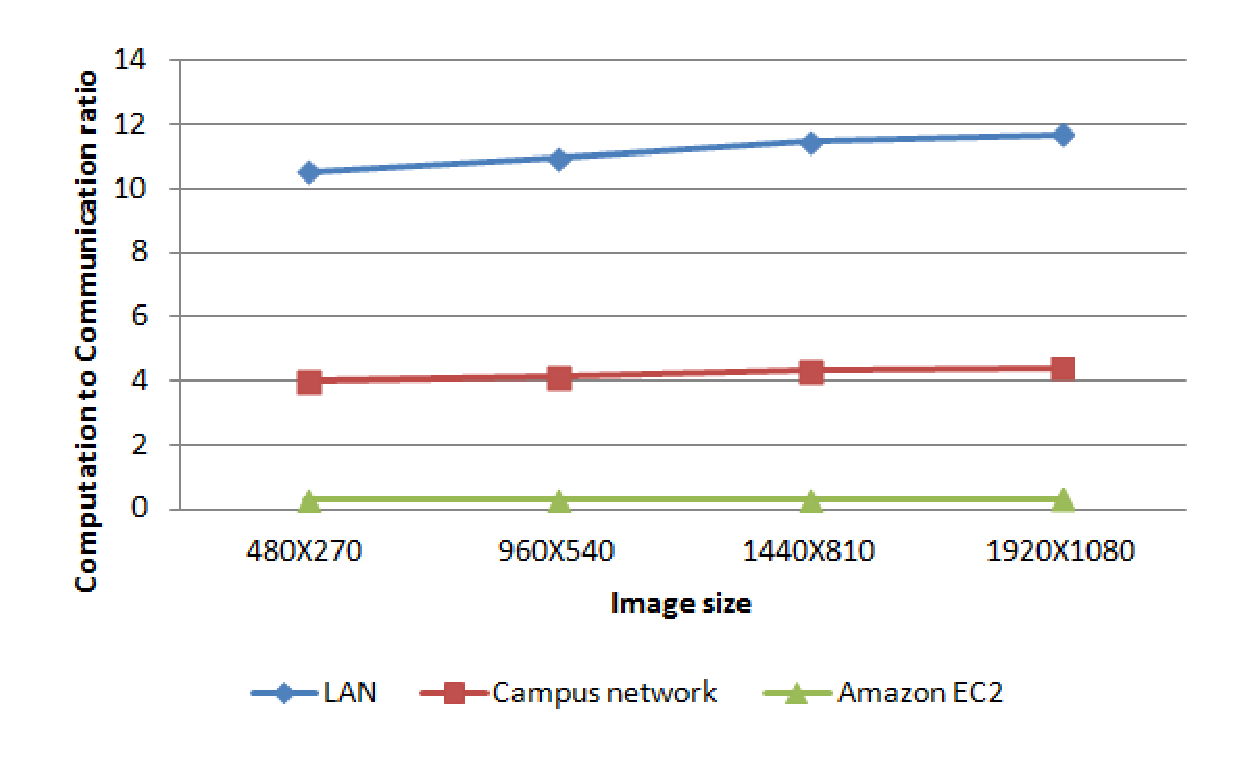
\epsfig{file=figs/ctoc_sobelfilter.eps, width=5.0in}
\caption{Computation to Communicaiton ratio for sobelfilter}
\label{fig:ctoc_sobelfilter}
\end{figure}
%
\begin{figure}
\centering
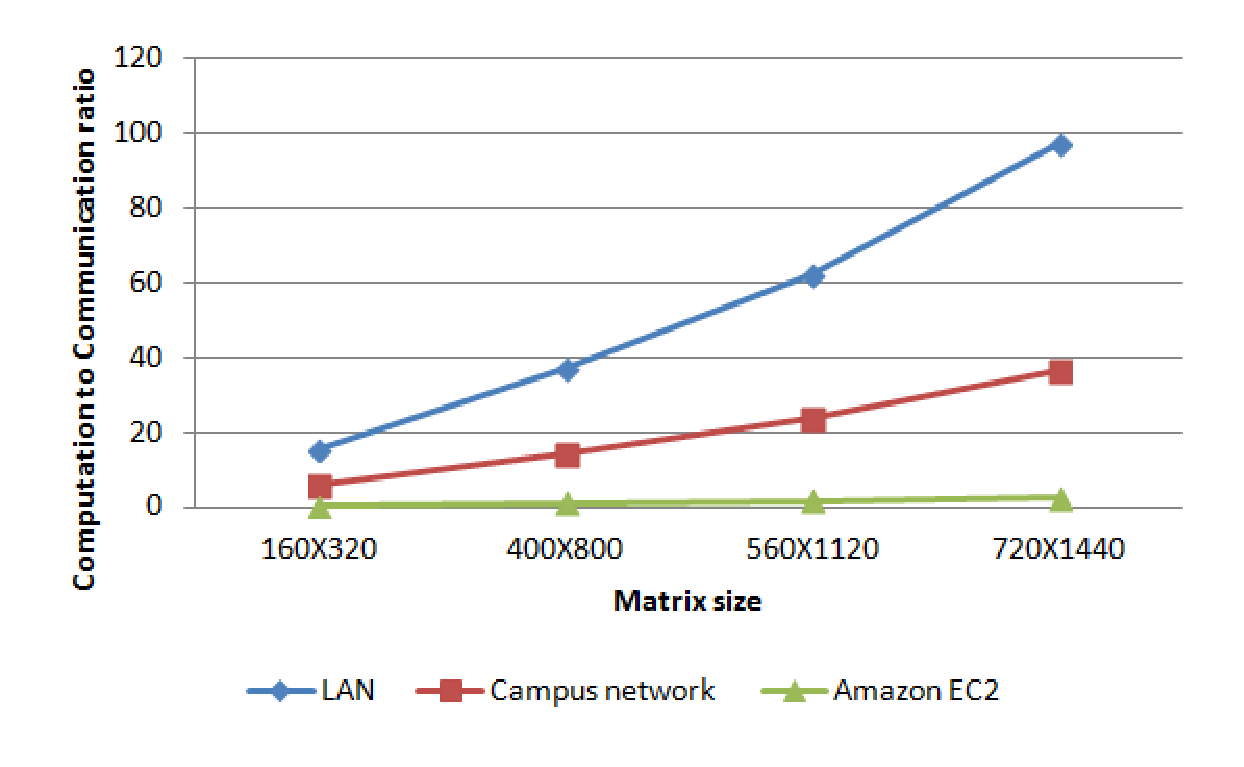
\epsfig{file=figs/ctoc_matrix.eps, width=5.0in}
\caption{Computation to communication ratio for matrix multiplication}
\label{fig:ctoc_matrix}
\end{figure}
%
\begin{figure}
\centering
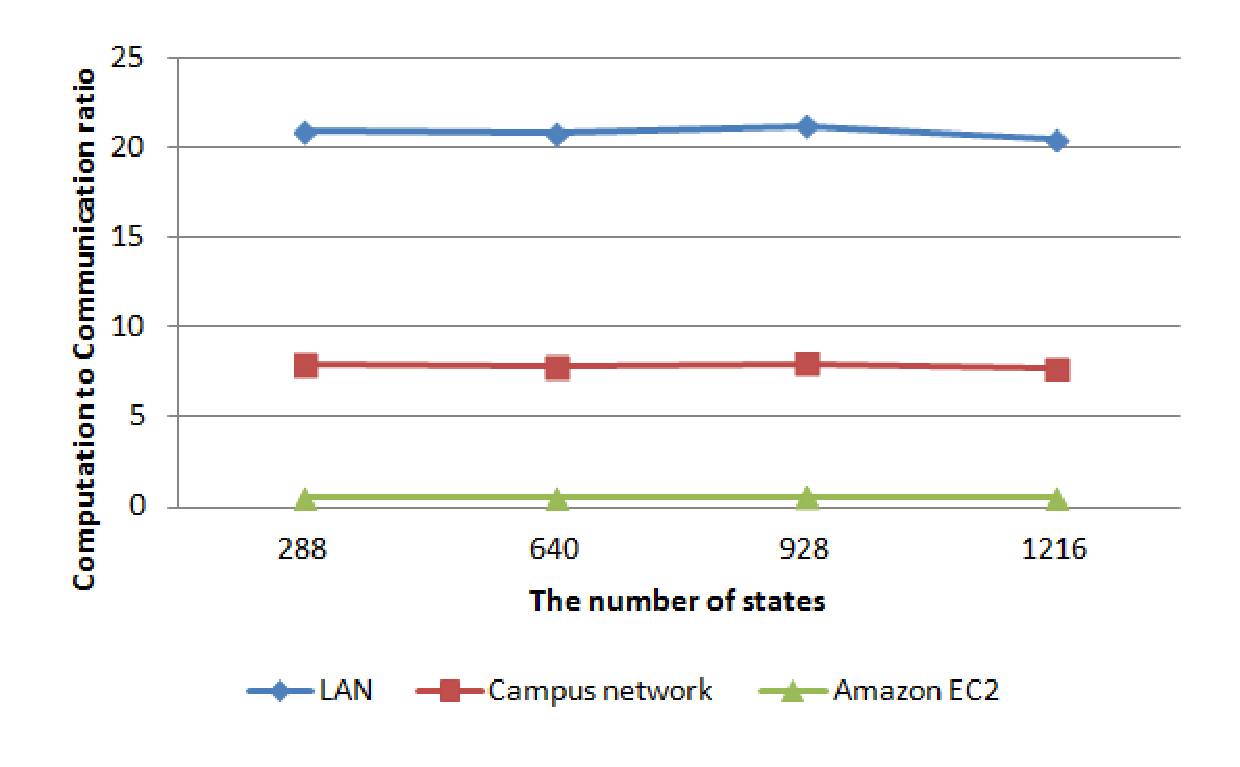
\epsfig{file=figs/ctoc_hmm.eps, width=5.0in}
\caption{Computation to communication ratio for hidden Markov model}
\label{fig:ctoc_hmm}
\end{figure}
%
\begin{figure}
\centering
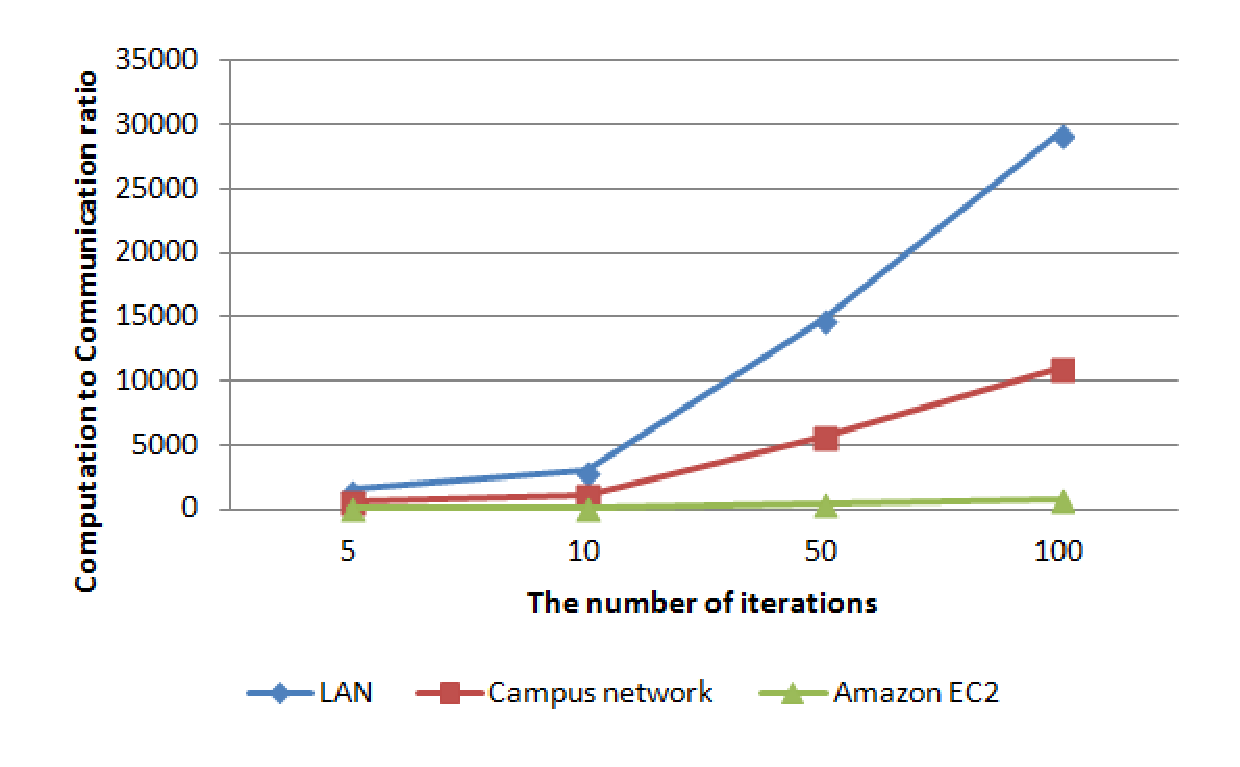
\epsfig{file=figs/ctoc_nbody.eps, width=5.0in}
\caption{Computation to communication ratio for {\it N}-body physics}
\label{fig:ctoc_nbody}
\end{figure}
%
\subsection{Offloading Performance}
\label{character:perf}
%
First of all, for sobelfilter, I observed better performance from
only a few cases where offloading 1440$\times$810 and 1920$\times$1080
of the image size to remote resources located in local area network
than local processing in Figure~\ref{fig:time_sobelfilter}. 
%
In fact, sobelfilter has lower computation to communication
ratios that other workloads ranging from 0.28 to 11.68 in the
experimental setup which indicates it is less computation-intensive 
(i.e. more communication-intensive) workload.
%
Especially, the cases of offloading to the resources located in campus
network and Amazon EC2 cluster instance whose computation to
communication ratio is fairly low have the worst performance in
sobelfilter.  
%
Also, I observed that better performance comes from more powerful
computing power by comparing CPU only-installed server and GPU installed
server in the same network configuration.
%
In contrast to sobelfilter, in all the cases of matrix
multiplication except for 160$\times$320 of matrix size, offloading is
much faster than local processing showing the speed-up which ranges from
1.2$\times$ to 9.2$\times$ as shown in Figure~\ref{fig:time_matrix}.
%
As mentioned in previous section, computation to communication ratios 
of matrix multiplication with the experimental setup range from 0.41 to 97.42 
which means that matrix multiplication is more computation-intensive workload 
than sobelfilter. 
%
Therefore, it is highly likely that matrix multiplication is able to
gain more from offloading to the remote resources with more powerful
computing capabilities.
%
In fact, the computation for matrix multiplication has higher complexity
than sobelfilter (the computation for matrix multiplication is
{\it O}($n^{3}$) while sobelfilter is {\it O}($n^{2}$)).
%
For the smallest matrix size of the setup, 160$\times$320, however,
I observed similar results as 1440$\times$810 and 1920$\times$1080 of
image size in sobelfilter where only offloading to resources in local
area networks has better performance than local processing.
%
With the results of sobelfilter and matrix multiplication, it is evident
that as computation to communication ratio becomes higher, 
it is possible to gain more from offloading.\\
%
Interestingly, in the cases of hidden Markov model, the
extremely worst performance is shown when the workload is offloaded to
Amazon EC2 GPU cluster which has the worst restrictions in terms of
network latency and bandwidth.
%
Though hidden Markov model has higher computation to communication
ratio than sobelfilter, the kernel for hidden Markov model is repeatedly executed 
requiring additional argument setups for each execution which incur 
more communication overhead as described in
section~\ref{character:workloads}.
%
In the Amazon EC2 setup, packets are sent or received at higher
latencies compared to the local area networks which impacts performance
especially since the OpenCL-based offloading framework requires that each RPC call is
acknowledged with a response from the server.
%
Consequently, offloading to Amazon EC2 GPU cluster, which has the
highest latency among the experimental setups, takes the longest time.
%
However, though {\it N}-body physics has the similar programming flow
as hidden Markov model, all the cases of offloading have better
performance than local processing because it is the most
computation-intensive workload among the experimental setup whose
computation to communication ratios range from 40.36 to 29323.68. 
%
\begin{figure}
\centering
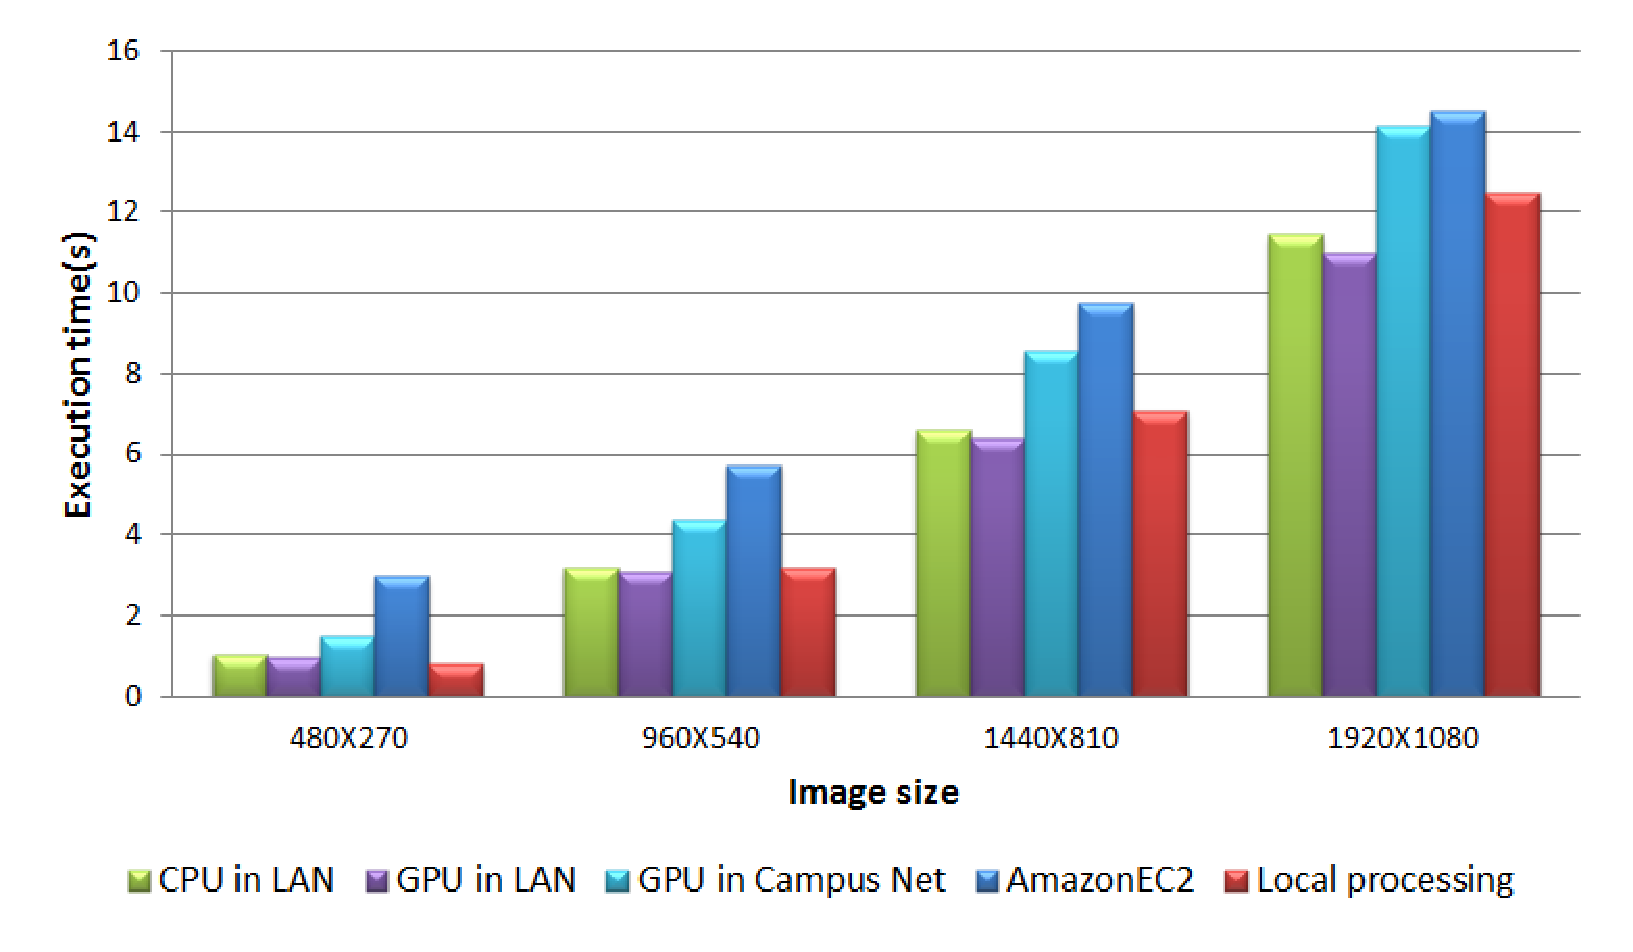
\epsfig{file=figs/time_sobelfilter.eps, width=5.0in}
\caption{Total execution time for sobelfilter with various
configurations}
\label{fig:time_sobelfilter}
\end{figure}
%
\begin{figure}
\centering
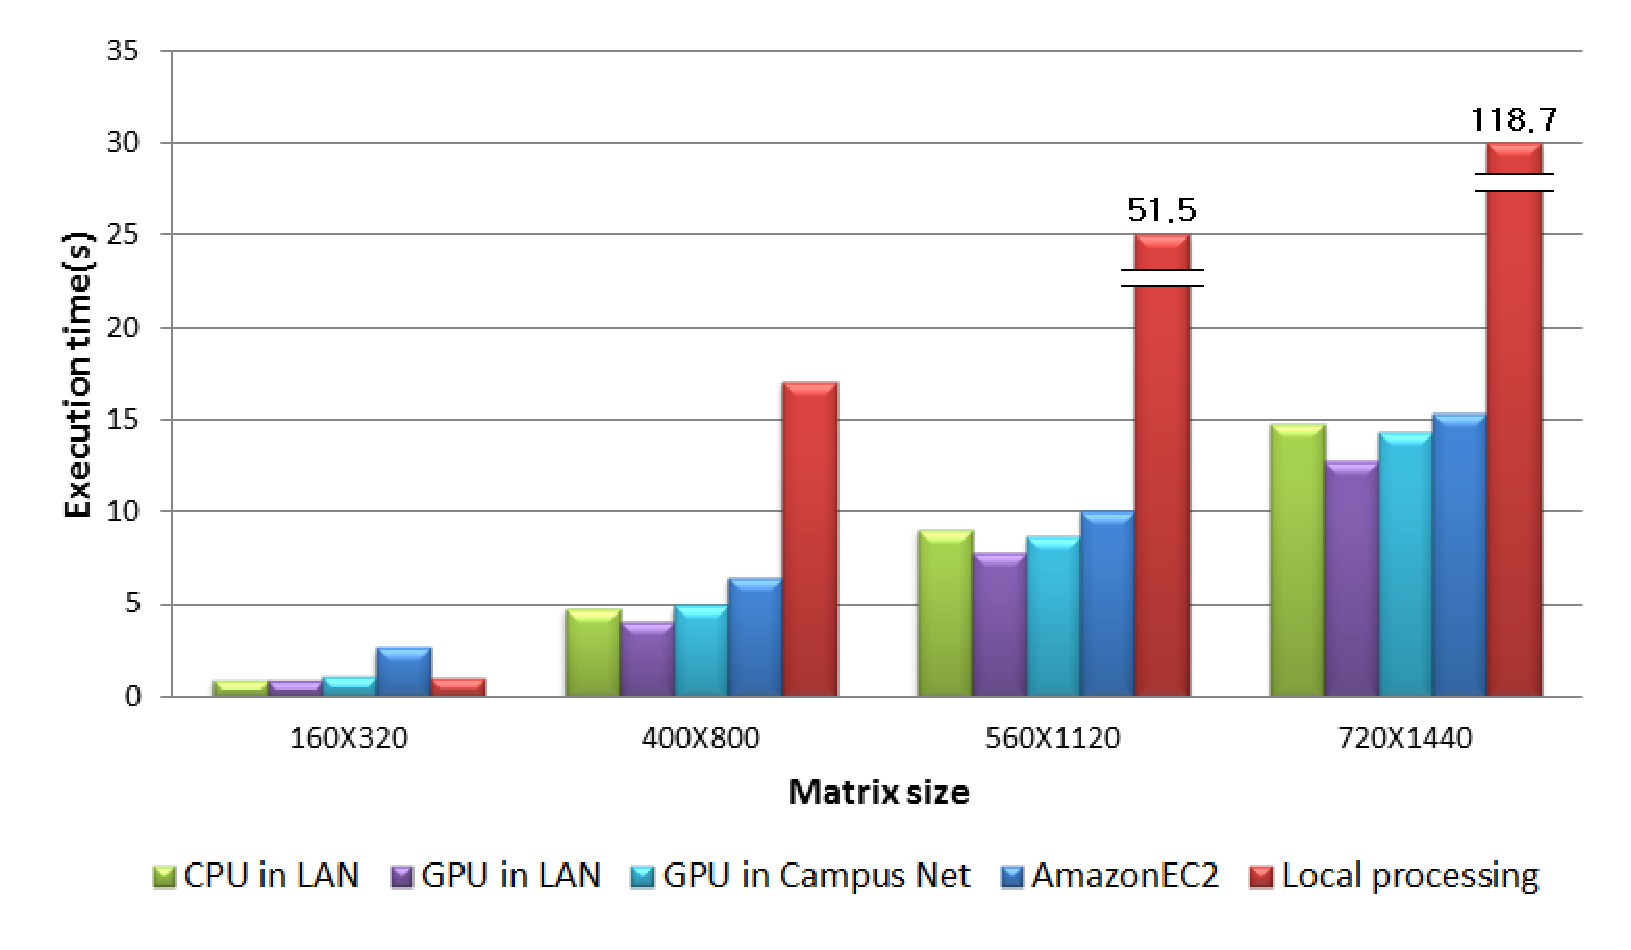
\epsfig{file=figs/time_matrix.eps, width=5.0in}
\caption{Total execution time for matrix multiplication with various
configurations}
\label{fig:time_matrix}
\end{figure}
%
\begin{figure}
\centering
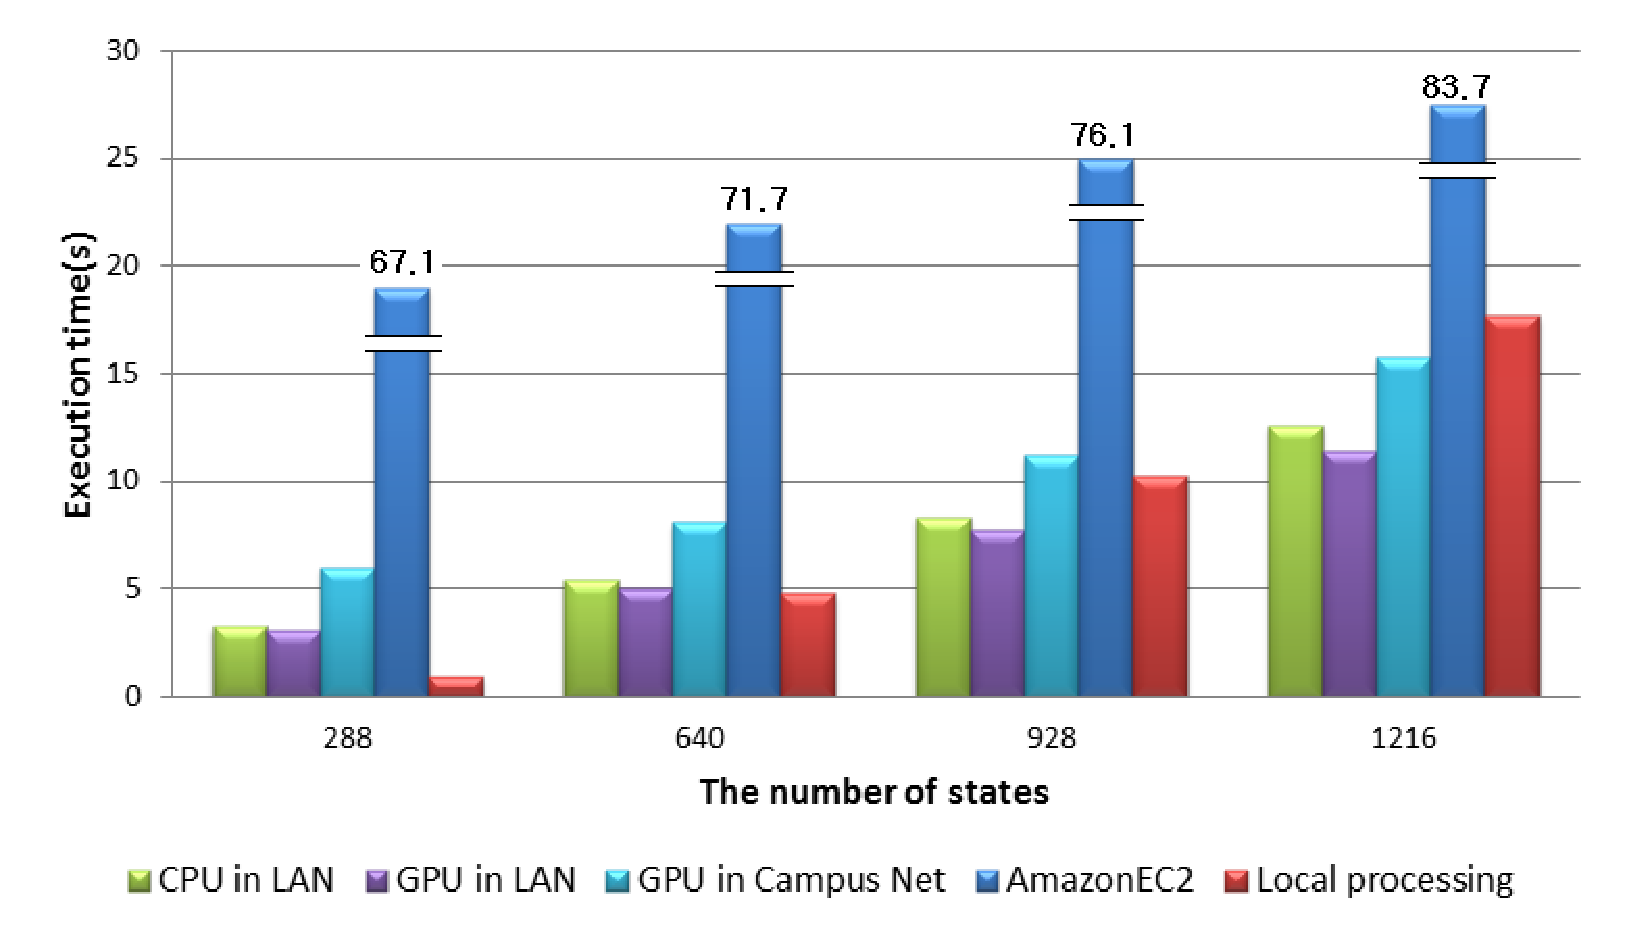
\epsfig{file=figs/time_hmm.eps, width=5.0in}
\caption{Total execution time for hidden Markov model with various
configurations}
\label{fig:time_hmm}
\end{figure}
%
\begin{figure}
\centering
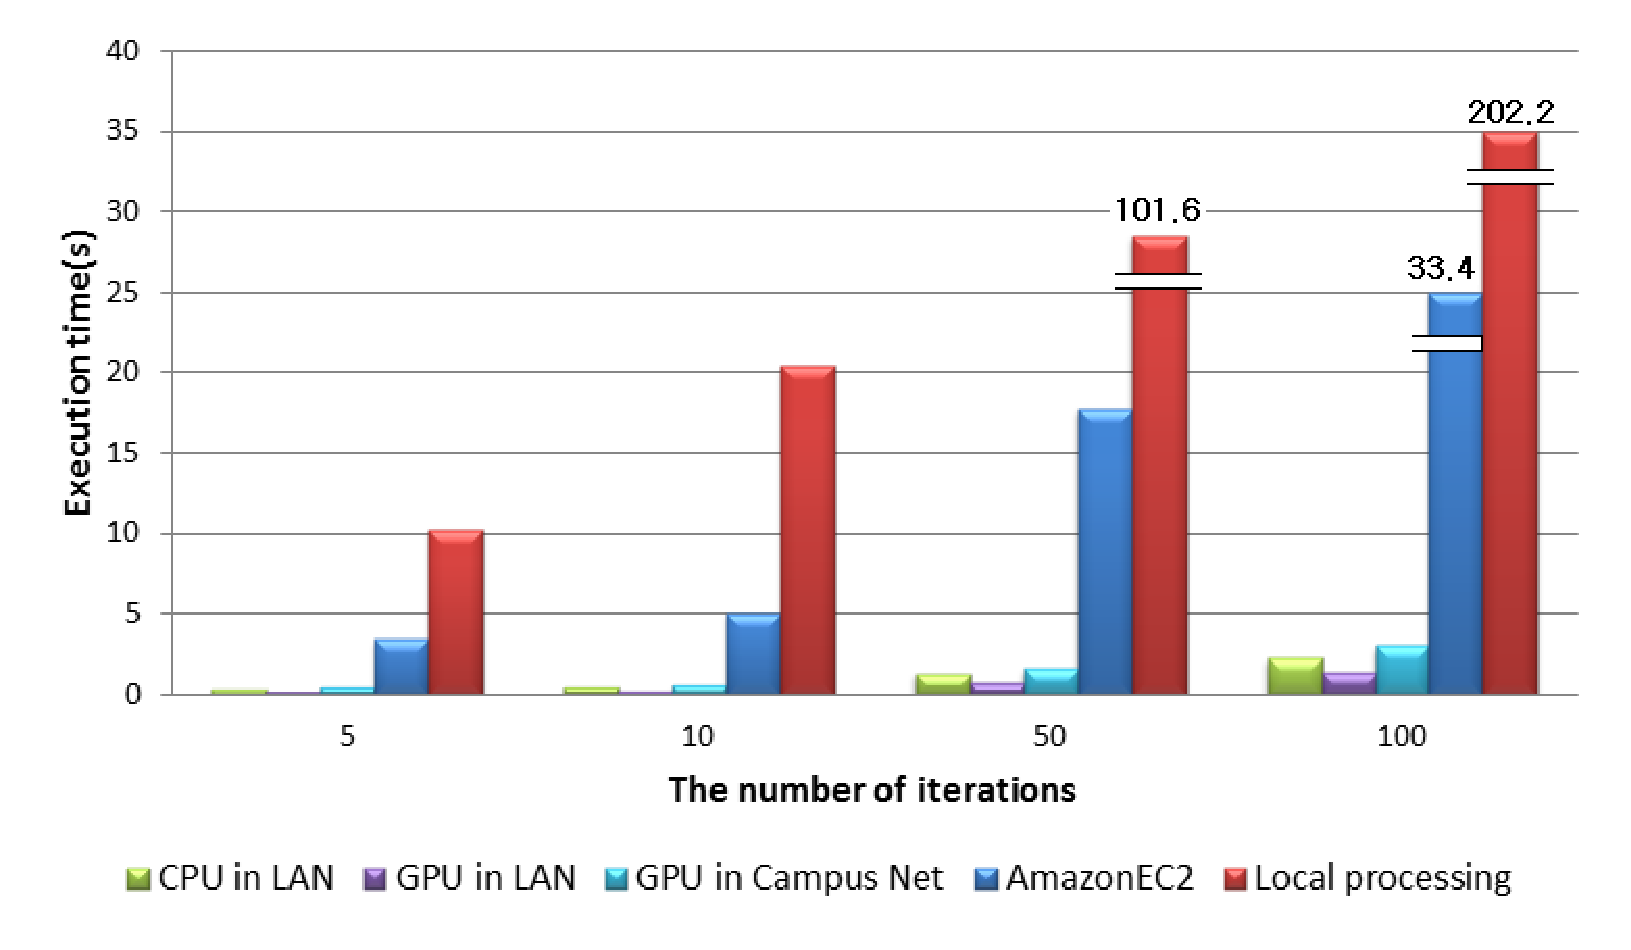
\epsfig{file=figs/time_nbody.eps, width=5.0in}
\caption{Total execution time for {\it N}-body physics with various
configurations}
\label{fig:time_nbody}
\end{figure}
%
\subsection{Energy Consumption}
\label{character:energy}
%
\begin{figure}
\centering
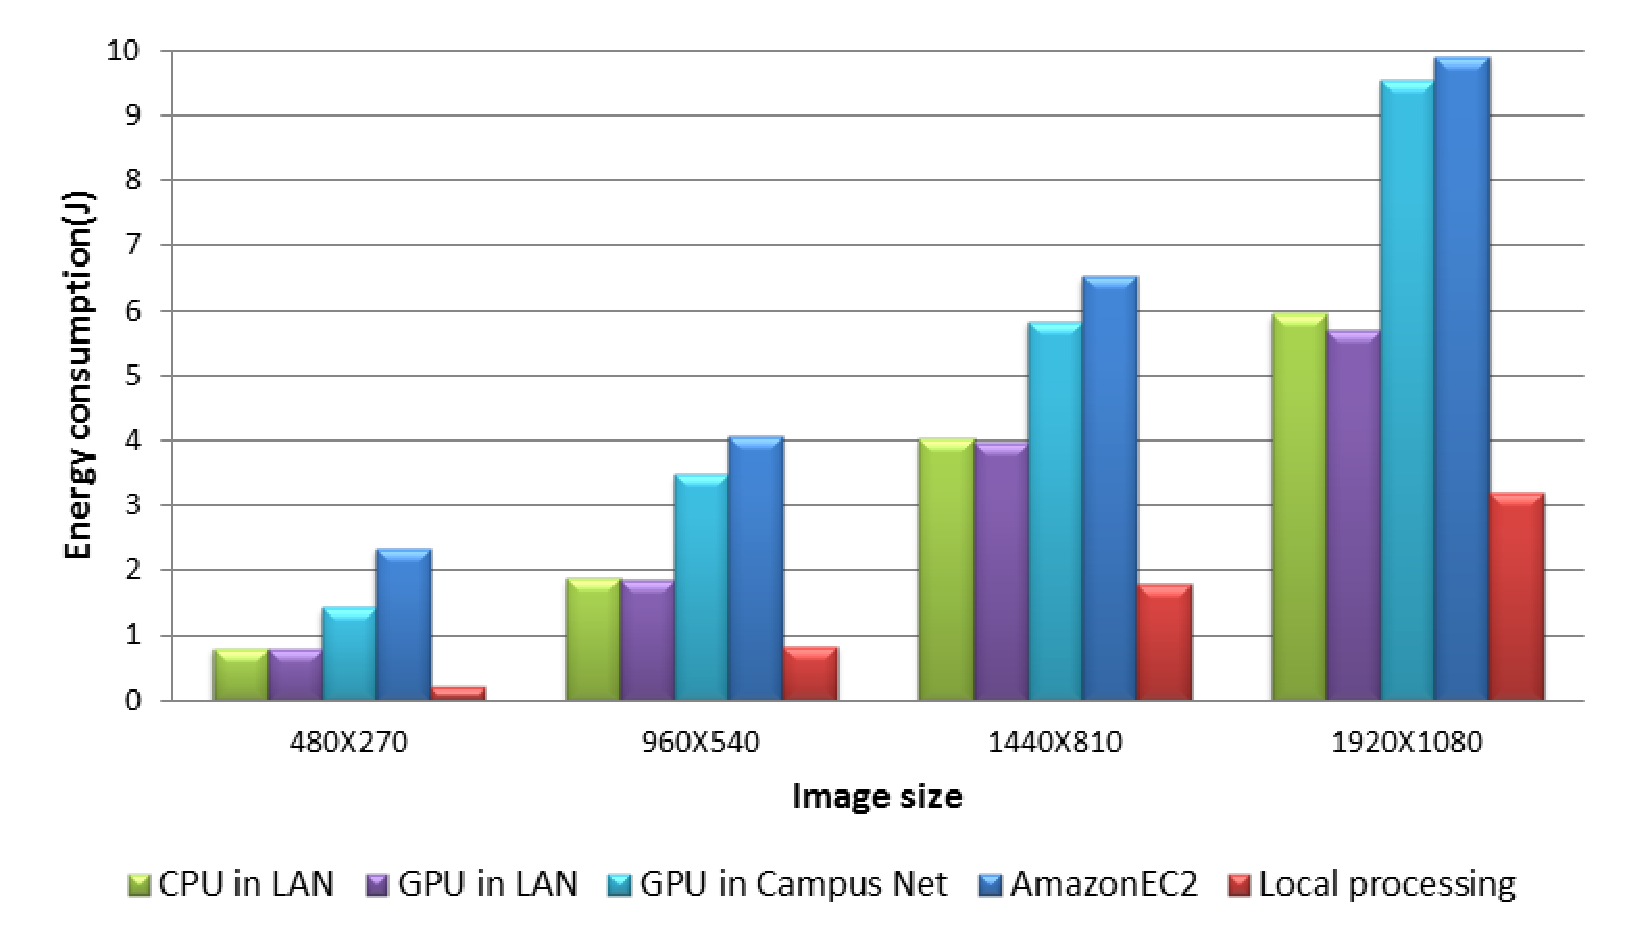
\epsfig{file=figs/energy_sobelfilter.eps, width=5.0in}
\caption{Energy consumption for sobelfilter with various configurations}
\label{fig:energy_sobelfilter}
\end{figure}
%
\begin{figure}
\centering
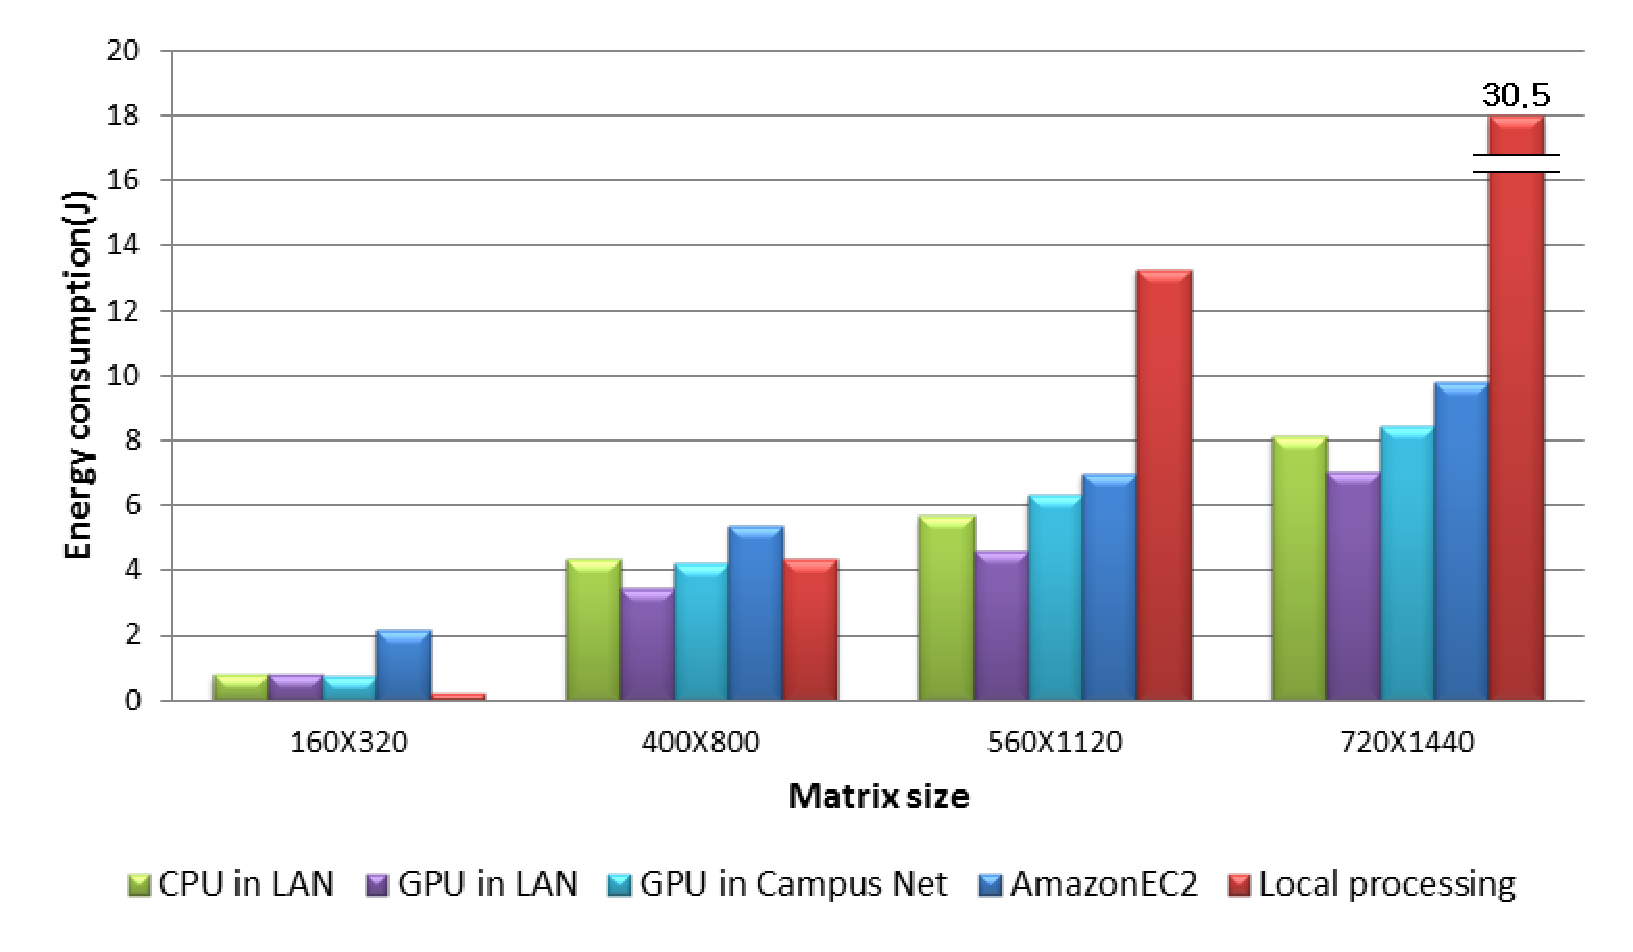
\epsfig{file=figs/energy_matrix.eps, width=5.0in}
\caption{Energy consumption for matrix multiplication with various
configurations}
\label{fig:energy_matrix}
\end{figure}
%
\begin{figure}
\centering
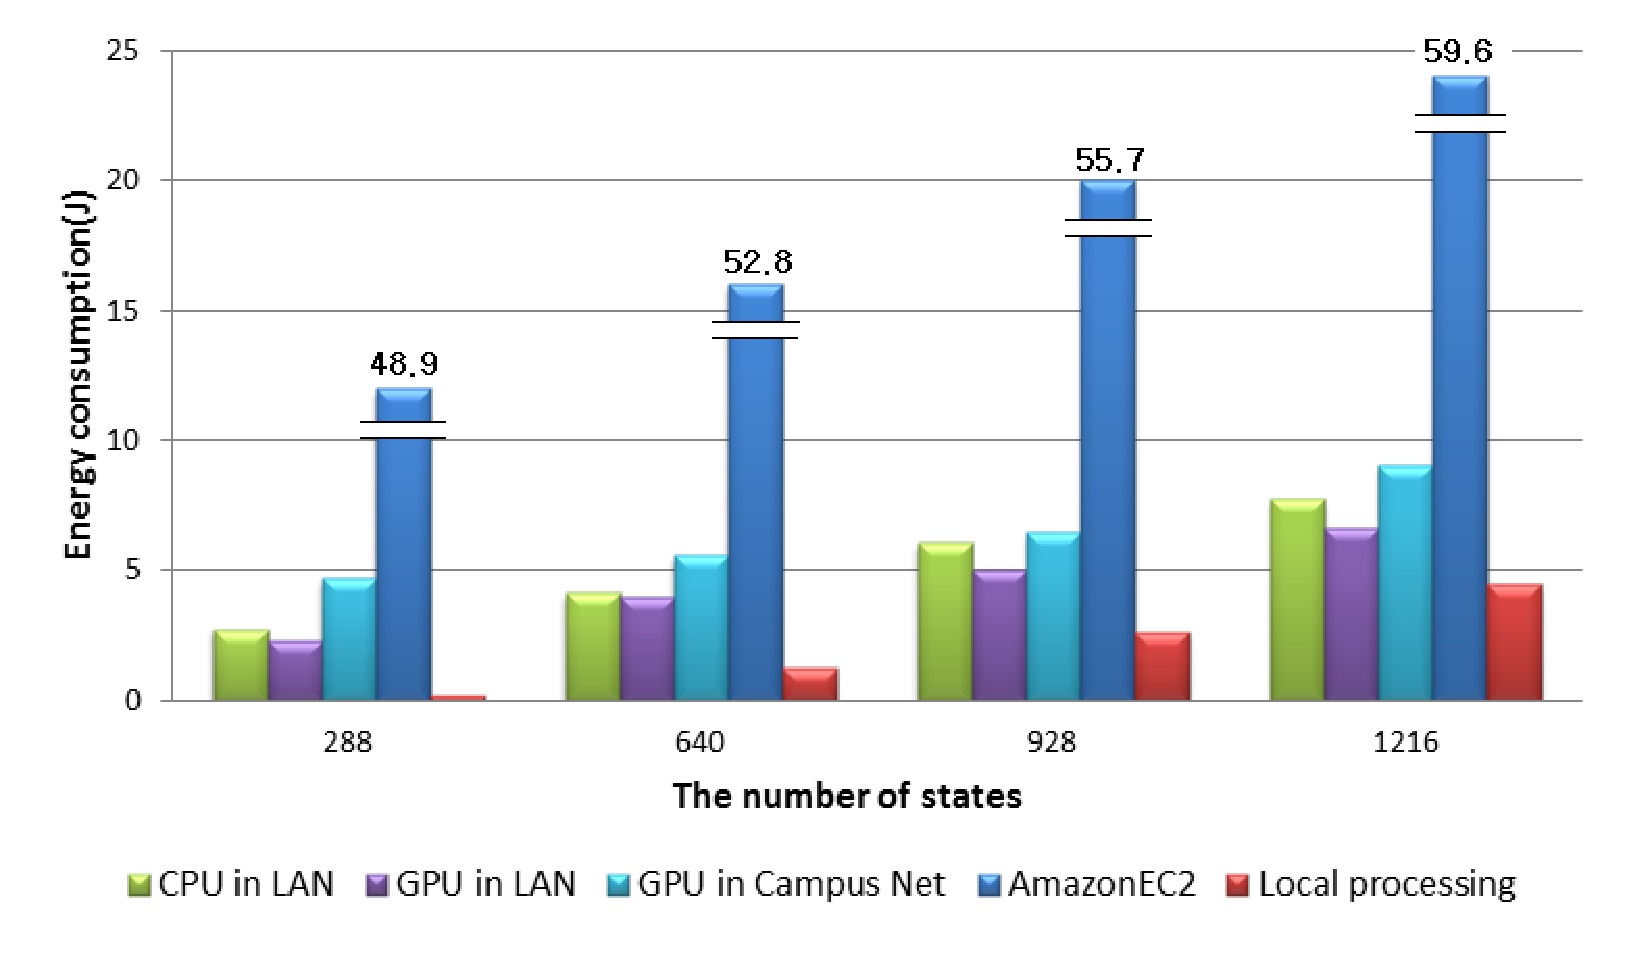
\epsfig{file=figs/energy_hmm.eps, width=5.0in}
\caption{Energy consumption for hidden Markov model with various
configurations}
\label{fig:energy_hmm}
\end{figure}
%
\begin{figure}
\centering
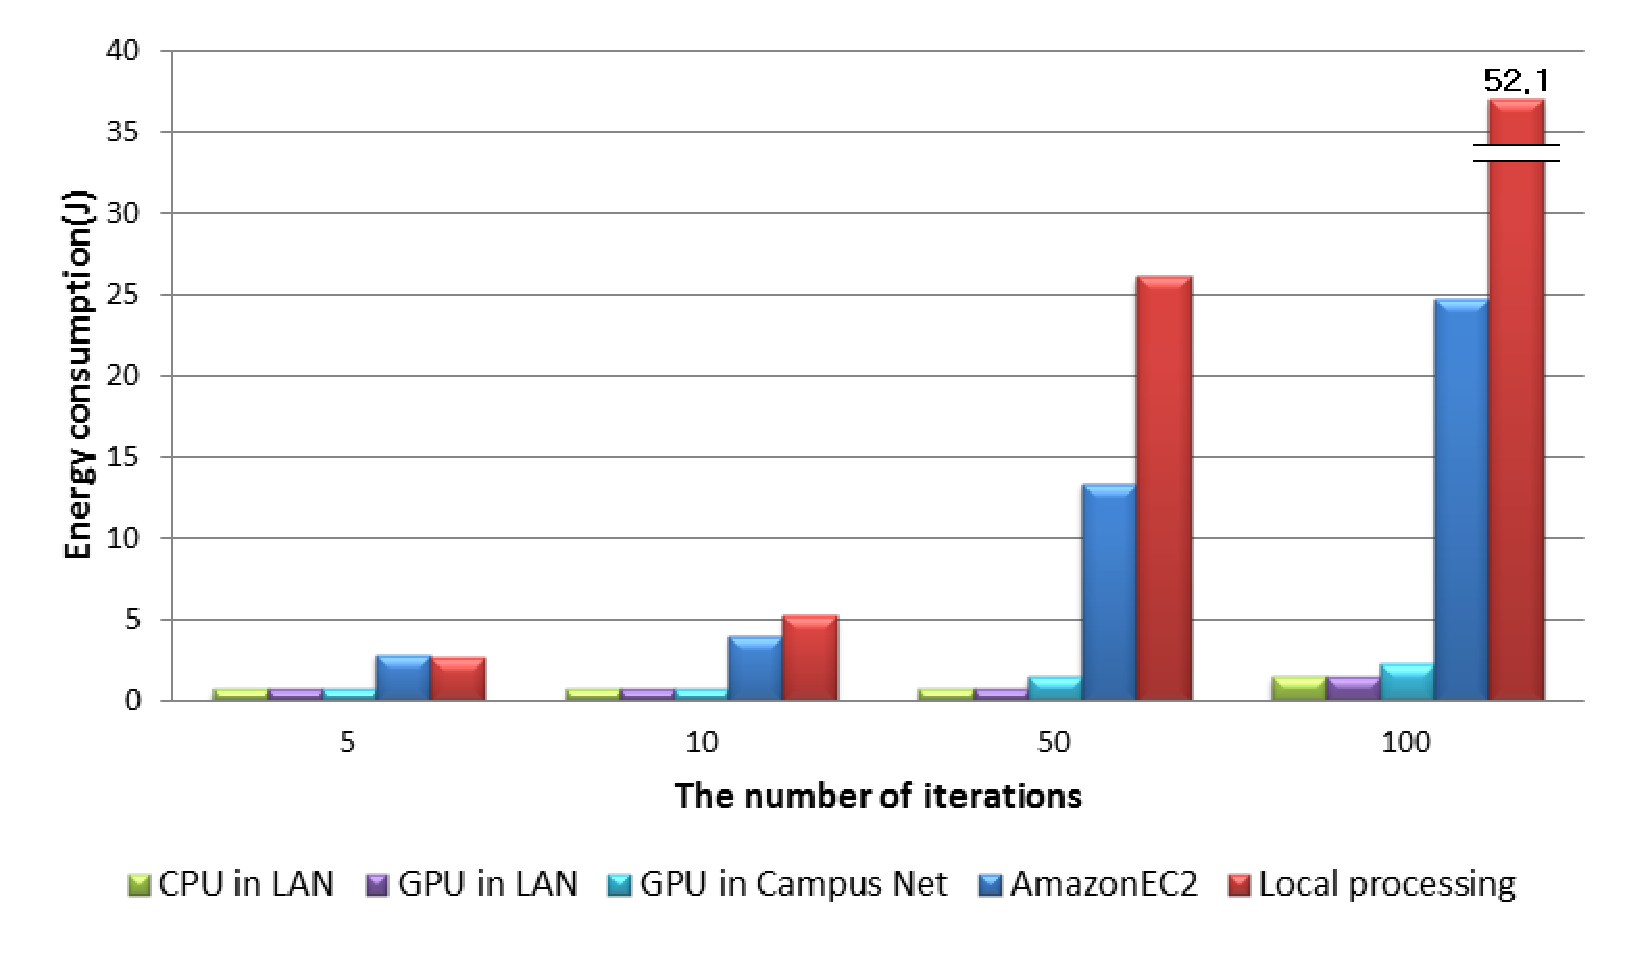
\epsfig{file=figs/energy_nbody.eps, width=5.0in}
\caption{Energy consumption for {\it N}-body physics with various configurations}
\label{fig:energy_nbody}
\end{figure}
%
To profile energy consumption of the mobile device, I used
PowerTutor~\cite{powertutor} which is an application for the variants of Android
devices that displays the power consumed by major components such as
GPU, network interfaces, LCD display, and GPS receiver.\\ 
%
A similar pattern for energy consumption of the mobile device as
the execution time is shown in
Figure~\ref{fig:energy_sobelfilter},~\ref{fig:energy_matrix},~\ref{fig:energy_hmm},
and~\ref{fig:energy_nbody}.
%
As computation to communication value is higher, 
it is likely that offloading is more beneficial than local processing.
%
However, it is worth noting that though some cases for sobelfilter
showed the benefits from offloading in terms of the execution time,
offloading consumes more than local processing as shown in Figure
3(a).
%
This dissimilar result comes from the discrepancy in the amount of power
consumed by CPU and the Wi-Fi networking card.
%
According to the measurement data profiled by PowerTutor, CPU consumes
200$\sim$220{\it mW} per second in active mode, while the
Wi-Fi networking card consumes about 710$\sim$720{\it mW}
per second in high power mode.
%
For that reason, even though offloading is faster than local processing,
it is possible that offloading consumes more energy than local
processing.
%
However, in matrix multiplication and {\it N}-body physics which
result in extremely high speed-up by offloading, it is observed that
offloading also improves energy implication as shown in
Figure~\ref{fig:energy_matrix} and~\ref{fig:energy_nbody}. 
%
\section{Summary}
\label{character:summary}
%
In this section, I analyzed the behavior of the mobile offloading
framework in terms of the offloading performance and energy implication
of the mobile devices with respect to characteristics of workloads and
environmental factors such as network conditions or the computing
capabilities of remote resources.
%
In order to characterize the workloads, I used computation to
communication ratio calculated by the local processing time divided by
the time for data transfer.
%
Furthermore, as part of the workload characterization effort, I
developed the OpenCL-based remote offloading framework by broadening the
scope of heterogeneity to include a new kind of platform component: the
computing capabilities on remote resources. 
%
I accomplish this by extending the well-defined hardware-level
offloading standard, OpenCL framework to support the various range of
remote computing elements over the network using the regular TCP/IP
network stack.
%
Also, I configured both local and wide area networks in which the
various computing capabilities are deployed to evaluate the impact of
environmental factors into the offloading performance.\\
%
According to the analysis, the benefits and the costs of the remote
offloading depend on computation to communication ratio as well as the
programming flow related to how the client and the server interact each
other.
%
In fact, as computation to communication ratio becomes higher, 
the performance improvement and the conservation of energy consumption 
also increase.
%
Moreover, in the cases of hidden Markov model and {\it N}-body
physics, I observed that the programming flow is also important to
analyze the behavior of the remote offloading for the mobile
platforms.  
%
I believe that the numerical results presented in this section guides the basis
of designing the intelligent runtime offloading scheduler which is
described in next section.

\chapter{MACHINE LEARNING-BASED RUNTIME SCHEDULER}
\label{chap:scheduler}
Rapid enhancements in computing capabilities of mobile platforms have
been driving the increased adopting and use of mobile computing
platforms by increasing numbers of users.
%
Today's mobile platforms are able to deliver capabilities that are close
to those of non-mobile platforms such as desktops or workstations.
%
For instance, a mobile phone equipped with a GPU core is able to achieve
approximately 10GFLOPS/Watt of compute-power, which is identical as a
4-core desktop with GPU~\cite{soyata}.
%
Despite of these significant advancements, mobile platforms remain
significantly limited by resources such as memory size, storage
capacity, and especially battery lifespan.
%
To alleviate the problem of the resource limitations in mobile
platforms, computation offloading techniques have been proposed as a way
to extend the capabilities of mobile platforms to more powerful
resources.
%
These may include personal computers, servers, or even public cloud
resource over the network~\cite{snarf, maui, cuckoo}.\\
%
However, the benefits from these systems can vary due to different
requirements for data transfer among various types of mobile
applications and dynamic network conditions including latency and
bandwidth.
%
As a result, offloading is not always beneficial, and poor offloading
decisions can result in the degradation of performance or energy
consumption.
%
Therefore, offloading frameworks need to consider the scheduling or
workloads onto remote or local processing resources adaptively, as a
function of network conditions and application requirements.\\
%
In this section, I address these challenges by considering machine
learning techniques for a runtime adaptive scheduler for mobile
offloading framework.
%
Machine learning technique is a branch of artificial intelligence
through which a system can learn from previous data and adapt to unseen
situations dynamically.
%
By applying machine learning techniques to the remote offloading
scheduling problem, a scheduler can be automatically trained from
previous offloading behaviors and make decisions on whether the mobile
workload should be offloaded or executed locally informed by past
behavior and current conditions.
%
There have been a number of related studies proposing adaptive
offloading mechanisms for mobile platforms.
%
To the best of our knowledge, this work is the first to systematically
study machine learning techniques for a mobile offloading scheduler.
%
To this end, I utilized the OpenCL-based offloading framework that I
explained in section~\ref{chap:offloading} and detailed measurement results
under various network conditions and mobile applications shown in
section~\ref{chap:character}.\\
%
One of the contributions described in section~\ref{chap:character} is
the combination of dynamic network conditions and application
requirements into {\it Computation to Communication ratio}, which considers
the local processing time for the workload, the amount of data transfer,
and network bandwidth.
%
The computation to communication ratio is a composite measurement which
coalesces three dynamic features into one parameter, and is used as an
attribute of the machine learning technique.
%
For the evaluation on the feasibility of applying machine learning
techniques to the adaptive scheduling problem, I utilized
{\it Weka}~\cite{weka}, a Java-based open source package.\\
%
After investigating the scheduling accuracy of several machine learning
algorithms using Weka, I choose a few machine learning algorithms which
have relatively high scheduling accuracy to implement an {\it offline}
offloading scheduler.
%
Further, by taking the complexity and scheduling performance into
account, I select Instance-Based Learning algorithm for an {\it online}
scheduler for mobile offloading framework.
%
In the evaluation, I show that although Instance-Based Learning online
offloading scheduler is fairly simple and has low overhead, it provides
performance advantages over non-adaptive schedulers for mobile
offloading system.
 
\section{Related Works}
\label{scheduler:relatedwork}
%
\subsection{Adaptive Mobile Offloading}
\label{scheduler:adaptive}
%
Many studies have considered adaptive mobile offloading
to provide performance improvements and energy savings for 
mobile platforms.
%
In~\cite{xiaohui}, the authors focus on relieving the memory limitation
of a mobile device by dynamically making the offloading decision with
Offloading Inference Engine (OLIE) which is based on the fuzzy control
model.
%
In particular, OLIE profiles the available memory size of a mobile
device and network bandwidth, and maps them into the offloading decision
specifications by the application developer, such that when the current
condition matches any specified rule, an offloading action is triggered.
%
In MAUI~\cite{maui}, the authors assume that offloading is always
preferable to local processing; however, it depends on three factors to
determine which methods should be offloaded to the remote server: the
device's energy consumption characteristics, the program characteristics,
and the network characteristics.
%
It established the relationship between CPU utilization and the energy
consumption of the mobile device and profiled the state transfer
requirement, runtime duration, and the number of CPU cycles.
%
Specifically, MAUI used the lightweight throughput measurement to profile
network condition.
%
With these information, MAUI schedules the local execution or offloading
at the beginning of the application to conserve the energy consumption
of the mobile platform.
%
In~\cite{shigeru}, a prediction model for the performance of
distributed mobile applications is evaluated through a sample image
processing application (i.e. face detection).
%
The prediction model heuristic uses linear functions to
approximate the time for local, remote execution and data transfer.
%
The server updates these functions using least-squares
method, and returns the updated heuristic linear functions to the client 
so that those updated functions are used for the performance comparison
between local processing and offloading.
%
Kovachev et al.~\cite{dejan} propose a simple cost function of
a service-based mobile cloud computing middleware for Android platforms
under three restrictions: minimized memory usage, minimized energy
usage, and minimized execution time.\\
%
Mobile "Grid" systems, where mobile devices participate as 
resource users or providers, also consider scheduling techniques to 
improve the performance of the systems while tackling the resource
constraints of mobile platforms.
%
In~\cite{waleed}, a novel energy-aware scheduling is
formulated and the level-based list scheduling heuristic is proposed for
a Mobile wireless Ad hoc NETwork (MANET).
%
The authors predefine the models for the task, the processor or the
mobile device, and the cost function, and the scheduler tries to
minimize the cost function by mapping each task to the resource through
the level-based list scheduling heuristic.\\
%
Ali et al.~\cite{hesham} present a mobile computing scheduling
mechanism based on self-ranking algorithm. 
%
Each worker node in the mobile grid system measures the connectivity and
utilization metrics and ranks itself using the ranking metric map from
the system developer.
%
Then, distributed tasks are assigned into high ranker nodes.\\
%
The distributed scheduler for the mobile grid system has
been proposed in~\cite{karin}.
%
Each mobile node self-evaluates its current and future capabilities
using static and dynamic device information such as connection quality,
remaining capacity and processor utilization, and it does matchmaking
the task requests similar to the Condor ClassAds.\\
%
Although the above-mentioned approaches take into account dynamic parameters
from the application level or the network level (i.e. CPU cycles,
network bandwidth) to predict system performance and schedule the mobile
workload execution, they still rely on predefined decision rules or cost
models, preventing the scheduler from adapting to dynamic conditions
during runtime.
%
In contrast, in this work, I consider approaches that do not rely on
any predefined specifications or prior knowledge of the mobile
application.
%
Instead, I consider machine learning techniques for adaptive runtime mobile
offloading schedulers.
%
Once trained with training data, the scheduler 
predicts the behavior of an incoming task when deciding on local or
remote execution.
%

\subsection{Machine Learning Techniques for Dynamic Scheduling Problems}
\label{scheduler:machine}
%
Machine learning techniques have been used to address dynamic scheduling
problems in various areas, such as heterogeneous computing platforms, grid
computing systems as well as in data center.
%
In~\cite{zheng}, machine learning techniques are used to provide a
compiler-based, automatic and portable predictor for multi-core
processors.
%
In order to determine the best number of threads and scheduling policy,
the authors used a feed-forward artificial neural network and a
multi-class support vector machine model, respectively.
%
Berral et al.~\cite{josep} propose an energy-aware
data center through server consolidation by turning off idle servers
with assistance from machine learning based scheduling.
%
The scheduler predicts the future performance of the jobs and power
consumption in the resulting job allocation using linear regression
algorithms.
%
The novel Adaptively Scheduled parallel R (ASpR) framework, which
transparently parallelizes scripts in the popular R language, is
presented in~\cite{jiangtian}.
%
This framework uses artificial neural networks for the performance
modeler which predicts task computation and data communication costs,
and this modeler is used by the directed acyclic graph to determine an
appropriate schedule.\\
%
In this work, I further consider the appropriateness of adopting
machine learning techniques to the scheduler of our mobile offloading
framework with respect to the complexity to construct the predictor and
ability to capture dynamic characteristics of mobile environments.
%
\section{Challenge for Adaptive Scheduling for Remote Offloading
Framework}
\label{scheduler:challenge}
In this section, I demonstrate the need for support from adaptive
runtime schedulers by conducting an experiment in which I deploy the
OpenCL-based remote offloading framework subject to various network
configurations and collect measurements to show the performance
disparity between different network configurations.\\
%
In the experiments, I utilized an Android tabletPC equipped with
1Ghz dual-core processor and 1GB RAM as a mobile client.
%
In order to observe the impact of different network
conditions on the offloading performance, I deployed a remote server
equipped with GeForce GT 640 graphics card into three different network
configurations: local area network, campus network, and Amazon EC2
instance.
%
In the local area network, I connected the mobile client and the remote
server through a wireless router supporting 802.11 b/g/n network
standard.
%
The campus network is used to represent a wide area network in which
the mobile client and the remote server are involved in different
networks: the mobile client connects to the campus wireless router and
the server connects to the laboratory internal router.
%
They communicate each other through multiple routers in the campus.
%
I used an Amazon EC2 GPU cluster as another option for the remote
server located in a wide area network, but for more restricted network
condition than the campus network.
%
Once again, Table~\ref{table:network_summary} in
section~\ref{character:setup} summarizes the average and standard deviation of latency
and bandwidth of the network configurations that I setup for the
experiments.\\
%
The benchmarks used in the experiment are sobelfilter, floating-point
matrix multiplication, Hidden Markov Model, and \textit{N}-body physics
provided by AMD APP SDK~\cite{amd} and NVIDIA~\cite{nvidia} sample code.
%
These execution kernels are used by a variety of applications in areas such as image
processing, physics simulation, and mathematical modeling.\\
%
\begin{figure}
\centering
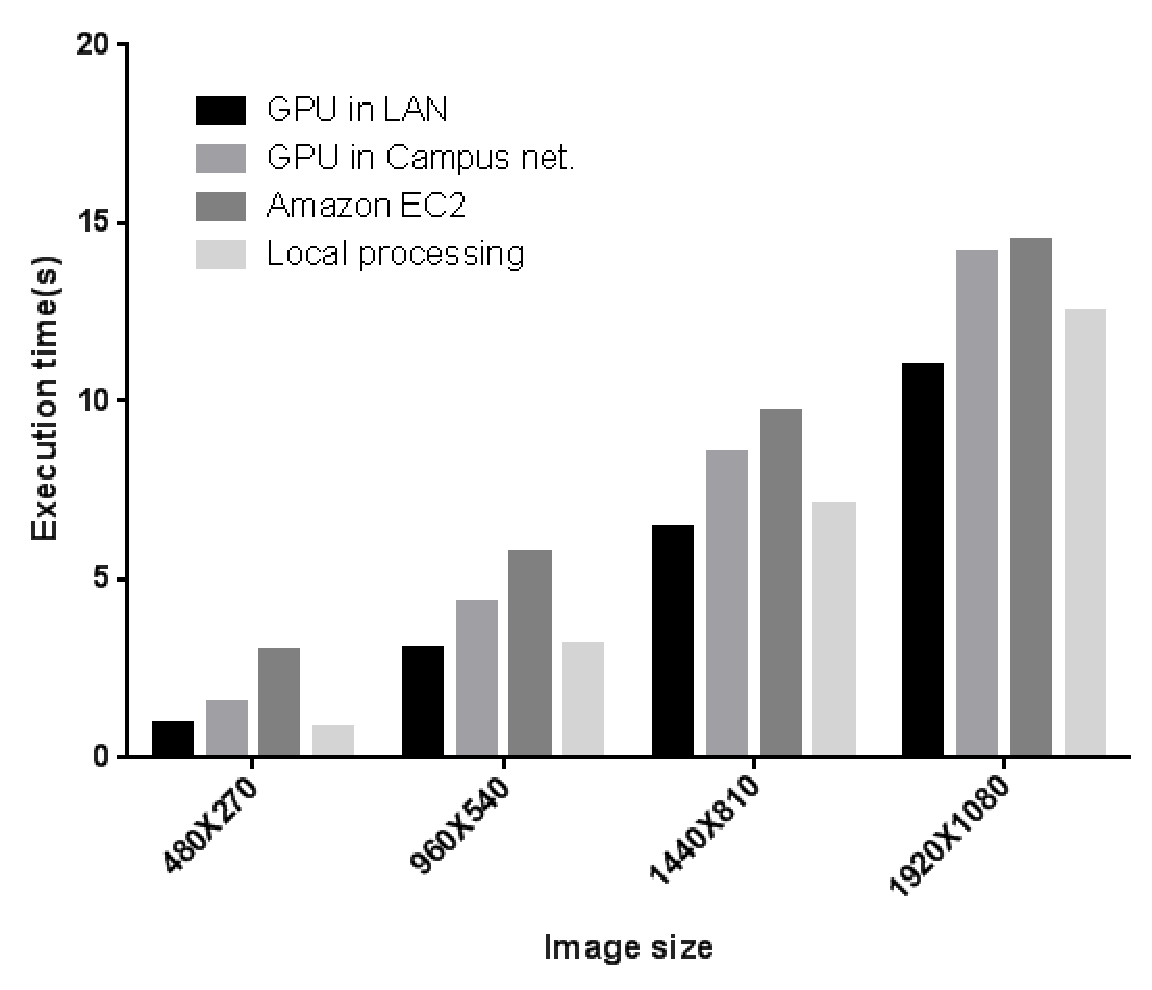
\epsfig{file=figs/challenge_network.eps, width=4.5in}
\caption{Performance for sobelfilter with various network
configurations}
\label{fig:challenge_network}
\end{figure}
%
\begin{figure}
\centering
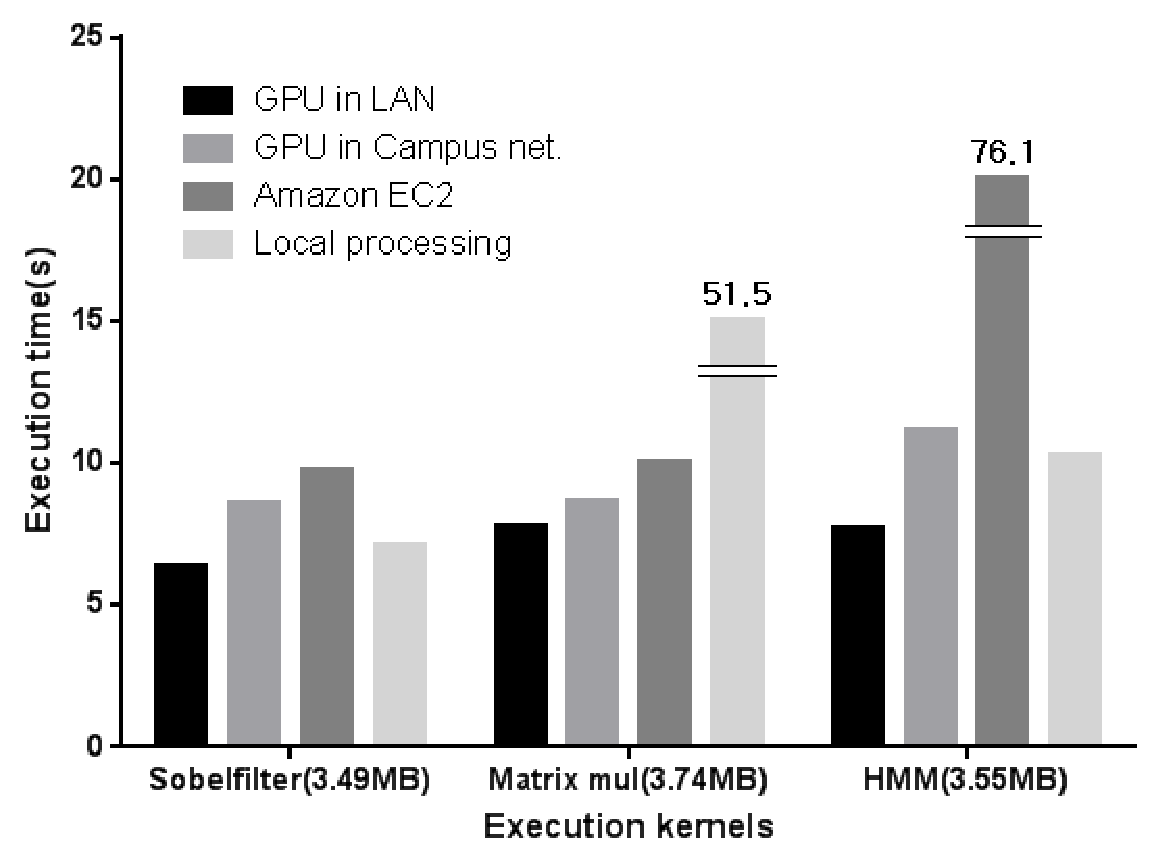
\epsfig{file=figs/challenge_workload.eps, width=4.5in}
\caption{Performance differences between various workloads}
\label{fig:challenge_workload}
\end{figure}
%
Figure~\ref{fig:challenge_network} and~\ref{fig:challenge_workload}
shows the offloading performance in terms of the
execution time compared to the case of local processing according to
the data size and network configurations for four OpenCL execution
kernels.
%
As shown in Figure~\ref{fig:challenge_network}, for sobelfilter, I observed that different
network conditions result in significantly different offloading
performance.
%
Particularly, offloading to the remote server located in a local area
network has better performance than local processing.
%
In contrast, offloading to the remote servers located in the campus network
and Amazon EC2 instance, where the offloading system has more restricted network conditions
than a local area network, takes longer time than local processing. 
%
Figure~\ref{fig:challenge_workload} shows the performance difference among various execution
workloads due to different computational requirements of workloads 
even though they process or offload the similar size of data ranging 
from 3.49MB to 3.74MB.
%
For sobelfilter, offloading to the GPU server located in LAN is only
more beneficial than local processing.
%
On the other hand, offloading floating-point matrix multiplication has
always better performance than local processing in our setup due to
heavier computational requirement of floating-point matrix
multiplication.
%
In fact, the computation complexity for floating-point matrix
multiplication is {\it O}($n^{3}$) while that for sobelfilter is
{\it O}($n^{2}$).\\
%
It is also worth noting that, for Hidden Markov Model, offloading to 
Amazon EC2 instance shows the worst performance among other cases.
%
This is because that Hidden Markov Model requires extra communications
between the mobile client and the remote server to setup additional
arguments for workload execution.
%
Packets are exchanged at higher latencies in the Amazon EC2 setup
compared with a local area network, which causes performance degradation
since our offloading framework requires that each RPC call is acknowledged 
with a response from the remote server.
%
Consequently, offloading to Amazon EC2 GPU instance, which has the
highest latency among our experimental setups, takes the longest time.
%
These results show that there is variation in offloading performance
between different network conditions and execution workloads.
%
Accordingly, proper scheduling can have a significant impact on the
offloading performance, and remote offloading framework requires the
support from the runtime scheduler.
%
\section{Machine Learning-Based Runtime Scheduler}
\label{scheduler:ml}
%
In order to apply machine learning techniques to any decision making
problems, it is first required to select a subset of relevant
attributes.
%
These need to comprehensively represent a set of problem instances in
terms of internal and external conditions which have an effect on making
a decision.
%
In this section, I describe the attributes of machine learning
techniques considered in this work, and how the proposed scheduler can
extract these attributes.
%
Then, using this subset of attributes, I investigate the scheduling
accuracy of machine learning techniques using a dataset collected from
experimental data using benchmark executions.
%
By taking the text-based dataset as an input, I can train the classifier
of various machine learning algorithms and examine the accuracy of the
trained classifiers.
%
\begin{figure}
\centering
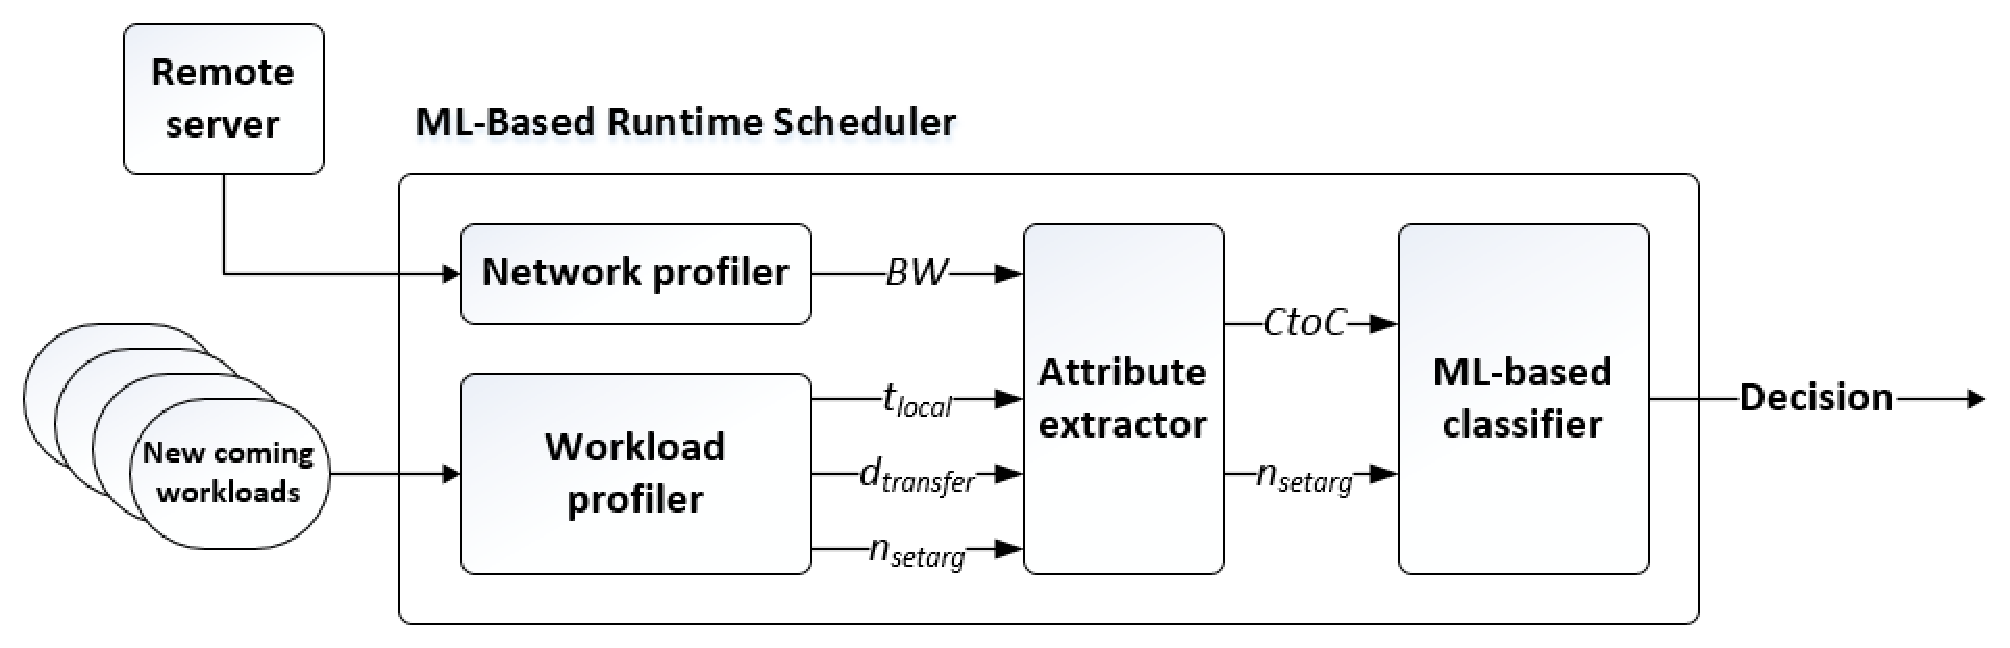
\epsfig{file=figs/scheduler.eps, width=5.5in}
\caption{Structure of machine learning-based runtime scheduler}
\label{fig:scheduler}
\end{figure}
%
Figure~\ref{fig:scheduler} illustrates the structure of the machine
learning-based runtime scheduler and how it generates and uses the
subset of attributes to make a decision for remote offloading framework.
%
\subsection{Selection of Machine Learning Attributes}
\label{scheduler:attributes}
%
Since offloading performance can vary as a function of network
conditions, the size of data to be processed, and computation
requirements, the scheduler has to take these factors into account to
make an accurate decision on offloading or local processing.
%
I focus on four features to establish the subset of attributes which is
the representation of the scheduling problem for the remote offloading
framework:1) computation amount of the workload, 2) size of data, 3)
network bandwidth, and 4) additional communication between the mobile
client and the remote resource to setup extra arguments.\\
%
{\bf Local execution time ({\it {t$_{local\_execution}$}}).} I regard the
time for a workload to be executed in the mobile client locally as the
computation amount.
%
There are a variety of methods to measure the computation amount of the
execution, such as counting the number of assembly instructions of loop
iterations, some of which require additional assistance from the
special hardware or compiler.
%
Instead, in the proposed approach, runtime measurements are taken by the
offloading framework as it executes the workload with the given data
locally, and the scheduler profiles the execution time for the
workload.\\
%
{\bf Data size to be transferred ({\it {d$_{transfer}$}}).} In addition
to the computation cost of a workload depending on the size of the data,
the data size also affects the communication cost to transfer the data
from the mobile client to the remote resource.
%
In the OpenCL-based remote offloading framework, the APIs for buffer
management such as {\it clEnqueueWriteBuffer} and {\it
clEnqueueReadBuffer} are used to profile the size of data to be
transferred.\\
%
{\bf Network bandwidth ({\it BW}).} I integrate the network bandwidth
measurement into the offloading framework so that it is able to measure
network bandwidth between the mobile client and the remote resource
during runtime.
%
In the implementation, network bandwidth is simply measured by the size
of probing packets divided by the elapsed time to send those
packets~\cite{bandwidth}.\\
%
{\bf Number of the invocations for argument setup ({\it
{n$_{arguset}$}}).} I count the number of the invocations of the specific
OpenCL API called {\it clSetKernelArgs}, which causes additional
communication overhead between the client and the remote resource to
setup the extra arguments for kernel executions in addition to the
primary data setup.
%
The reason why I distinguish communications between main data transfer
and additional arguments setup is that, though the latter incurs minor
amount of data, it can cause significant communication costs due to
protocol round-trip messages between the client and the remote
resource.\\
%
Not that, rather than considering the local execution time, the size of
data transfer, and network bandwidth as individual attributes
separately, I use {\it Computation to Communication ratio} in which
three features are merged into one attribute as Equation~\eqref{equ:ctoc}.
%
\begin{equation}
\begin{split}
	CtoC& = t_{local\_execution}\:/\: t_{data\_transfer} \\
	& = t_{local\_execution}\:/\:(d_{transfer}\:/\:BW)
\end{split}
\label{equ:ctoc}
\end{equation} 
%
where {\it t$_{data\_transfer}$} is the time for data transfer.
%
Thus, in this work, computation to communication ratio is a composite
measurement which combines three dynamic features into one parameter.
%
As a result, the proposed machine learning-based classifier accepts two
attributes: computation to communication ratio({\it CtoC}) and the
number of invocations of {\it clSetKernelArgs}({\it n$_{argset}$}) to
make a decision on scheduling a new workload(i.e. local processing or
remote offloading).
%

\subsection{Scheduling Accuracy of Machine Learning techniques}
\label{scheduler:accuracy}
%
In this subsection, I investigate the scheduling accuracy of the machine
learning-based scheduler for remote offloading framework.
%
First of all, by running the OpenCL-based offloading framework into the
experimental setup with various network configurations, execution
kernels, and data sizes as described in
section~\ref{character:methodology}, I gathered a total 640 data
instances to train and test the classifiers of various machine learning
algorithms.
%
Each data instance means one execution of the offloading framework, and
consists of \{{\it d$_{transfer}$}, {\it BW}, and {\it n$_{argset}$}\}.
%
Next, I aggregate collected data instances to create the training and
test datasets, each consisting of a 3-tuple, {{\it CtoC}, {\it
n$_{argset}$} ; {\it label}}, with two attributes explained in
section~\ref{scheduler:attributes} and the label which is a decision on
{\it offload} or {\it local}.
%
\begin{figure}
\centering
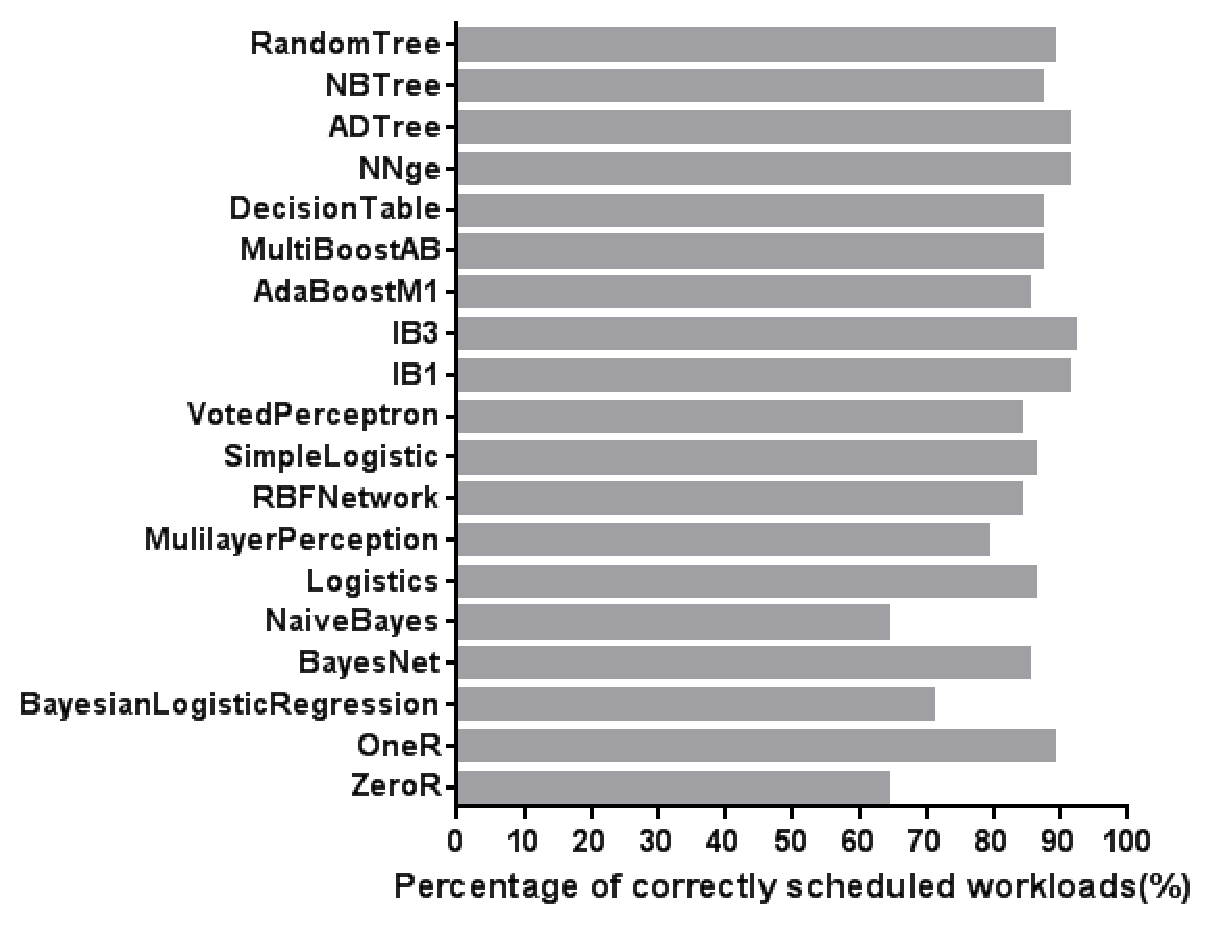
\epsfig{file=figs/scheduling_accuracy.eps, width=4.5in}
\caption{Offloading scheduling accuracy of various machine learning
algorithms}
\label{fig:scheduling_accuracy}
\end{figure}
%
Then I labeled each data instance by comparing offloading 
performance to the local execution in terms of the execution time.
%
For example, if offloading sobelfilter with a 1920$\times$1080 image
into a machine with a GPU in LAN takes a shorter time than
local processing, the instance is labeled as \textit{offload}.
%
In the collected dataset, 65\% of instances are labeled as
\textit{offload}.
%
Note that it is possible to use another performance metric: mobile
device's energy consumption, such that each instance can be labeled
based on energy consumption between remote offloading and local
processing.
%
Lastly, I separated the collected dataset with 70\% of them for
the training dataset and the rest for the test dataset, so they have
the identical distribution for instance properties.\\
%
Using the training dataset, I trained the classifiers of various
categories of machine learning algorithms such as Decision Tree,
Bayesian Networks, Instance-Based Learning, and Perceptron-Based
Learning. 
%
In the training phase, Weka takes the text-based training dataset as
the input and automatically generates the classifier associated with
each machine learning algorithm.
%
Once each classifier is trained, I tested the accuracy of the
trained classifier with the test dataset by observing whether the
trained classifier labels each instance in the test dataset correctly or
not.\\
%
Figure~\ref{fig:scheduling_accuracy} shows the scheduling accuracy of
various machine learning algorithms.
%
In this evaluation, the scheduling accuracy is calculated through the
number of the correct decisions made by the classifier out of the test
dataset.
%
I observed that two Instance-Based Learning classifiers performed 
the most accurate prediction, showing greater than 90\% of the scheduling
accuracy.
%
The basis for the classification of Instance-Based Learning is the instances 
database, where previously seen instances are stored.
%
Instead of building the explicit classifier as other machine learning
algorithms, Instance-Based Learning compares a new problem instance with the stored
instances in the database to select {\it k} most similar instances 
from the database and votes the majority of the selected instances to 
predict the label of the new problem instance.
%
{\it k} set to 1 (IB1) and 3 (IB3) as higher values showed the same
performance. 
%
The classification of probabilistic machine learning
techniques such as Bayesian Networks is based on the statistics
of attributes of the previous instances such as the mean and the
variance values.
%
Thus it is possible that probability-based machine learning
algorithms overlook the edge of previously seen instances, which causes
the performance degradation for the prediction problem. 
%
In fact, Naive Bayes has the worst performance among machine learning
algorithms used for the evaluation, showing 64.4\% scheduling
accuracy.
%

\section{Performance Evaluation for Offline Scheduler}
\label{scheduler:offline}
%
In this section, using the classifiers from various machine learning
algorithms, I implement an offline offloading scheduler and evaluate
the performance and penalty of the offline runtime schedulers.
%

\subsection{Experimental Setup}
\label{schedeulr:offline_setup}
%
Based on scheduling performance and algorithm complexity, I selected
three machine learning algorithms: RandomTree, Instance-Based Learning
and Rule-Based Learning, and built them onto our remote offloading
framework for the offline runtime scheduler.
%
For RandomTree, I used the classifier that Weka generated using the
training dataset described in section~\ref{scheduler:accuracy}.
%
Total depth of the tree is 101 and the scheduling accuracy simulated
through Weka is 89.5\%.\\
%
Though I do not need any classifier for Instance-Based Learning
algorithm, it is required to define the similarity between a new problem
instance and previously stored instances in the database.
%
To do this, I used Euclidean distance, which is common to measure the
similarity for Instance-Based Learning~\cite{instance}.
%
The closer the distance between instances is, the more similar 
they are.
%
I stored the training dataset with 448 instances to build the
database for the Instance-Based Learning algorithm.
%
For simplicity, I use {\it k=1} for Instance-Based Learning
algorithm.
%
For Rule-Based Learning, I establish a simple rule based on
computation to communication ratio threshold, in which the scheduler
decides to offload the mobile computation only if
computation to communication ratio is higher than the threshold.
%
Based on our observation, it is most likely that the benefits from
offloading are more promising when computation to communication ratio is
higher than 1.5.
%
For that reason, I setup the threshold with 1.5 and 3.\\
%
Also, I emulate various network configurations in which the
client and the server connect directly through a wireless router, but
have 9 different network bandwidths ranging from 6.5MB/s to 0.3MB/s
controlled by Traffic Control (TC)~\cite{tc}.
%
TC is a network tool which provides functionalities to control network
traffic by prioritizing network resources and using concepts of traffic
classification, queue disciplines and quality of service (QoS).
%
While setting different network bandwidths, I ran
our offloading framework with four benchmark kernels 720 times (9
network bandwidths $\times$ 4 kernels $\times$ 4 data sizes $\times$ 5
repeats for average) per each offline scheduler.
%

\subsection{Performance Comparison}
\label{scheduler:offline_perf}
%
\begin{figure}
\centering
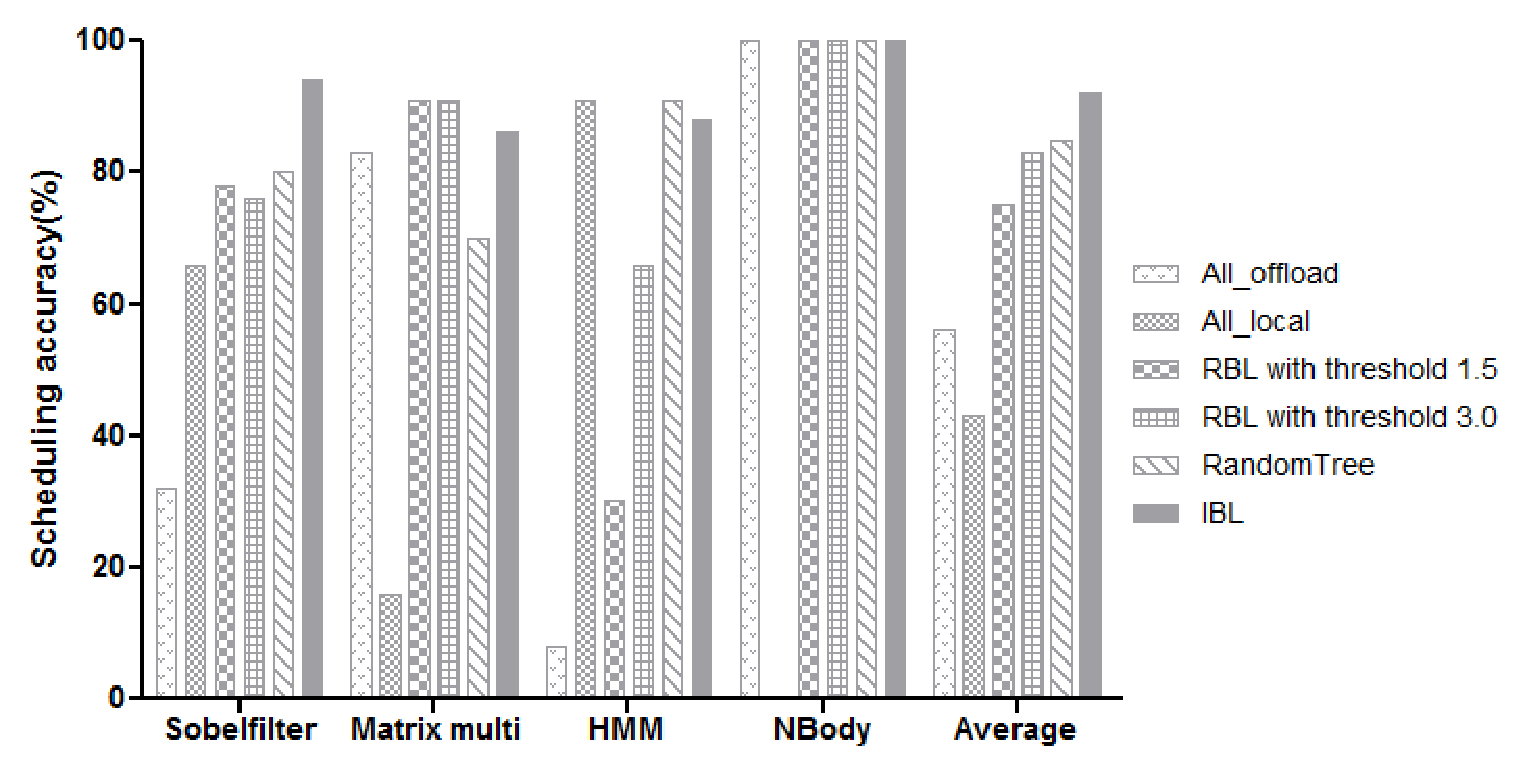
\epsfig{file=figs/offline_accuracy.eps, width=5.5in}
\caption{Scheduling accuracy of offline schedulers}
\label{fig:offline_accuracy}
\end{figure}
%
Figure~\ref{fig:offline_accuracy} shows the scheduling accuracy for various machine learning
algorithms with four benchmark kernels.
%
Similarly as the result shown in Figure~\ref{fig:scheduling_accuracy}, I observed that
Instance-Based Learning has the most accurate scheduling performance
among various schedulers showing 92\% of the scheduling accuracy.
%
Even though in matrix multiplication and Hidden Markov Model,
other machine learning algorithms have better performance than Instance-
Based Learning, Instance-Based Learning shows the best performance on average.
%
It is also observed that, even though the schedulers based on Rule-Based
Learning algorithm consider only one attribute,
computation to communication ratio, they have better performance than
RandomTree.
%
An interpretation is that the computation to communication ratio is a
more dominant attribute than the number of argument setup, {\it n$_{argset}$}.
%
Interestingly, for {\it N}-body physics, all machine learning
algorithms show the perfect scheduling accuracy.
%
It is because that computation to communication ratio for
{\it N}-body physics is extremely high in our experimental setup
so that it is easy for the scheduler to differentiate the conditions 
where offloading or the local execution for {\it N}-body physics 
is more beneficial than the other.
%
In fact, offloading {\it N}-body physics always had better
performance that the local execution in the experimental setup.\\
%
Figure~\ref{fig:penalty_time} and~\ref{fig:penalty_energy} 
present the penalty for various schedulers
normalized to the case of the oracle scheduler which always makes the
right decision to offload or run locally as Equation~\eqref{equ:penalty}.
%
\begin{figure}
\centering
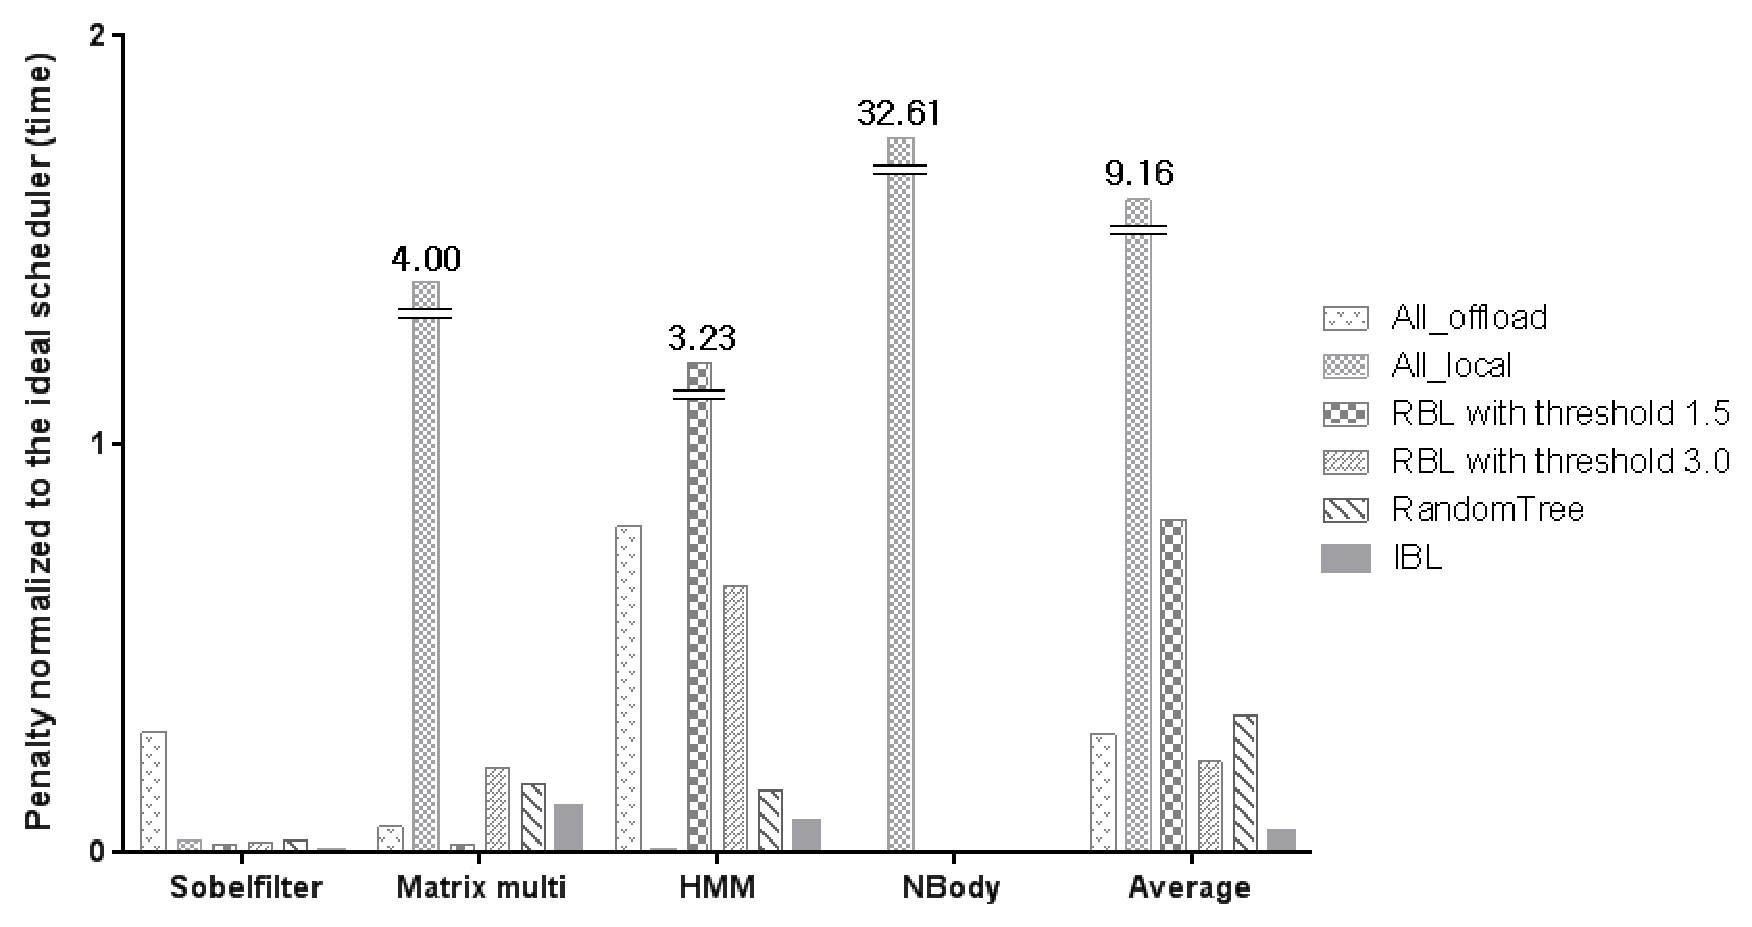
\epsfig{file=figs/penalty_time.eps, width=5.5in}
\caption{Penalty(execution time) normalized to the oracle scheduler}
\label{fig:penalty_time}
\end{figure}
%
\begin{figure}
\centering
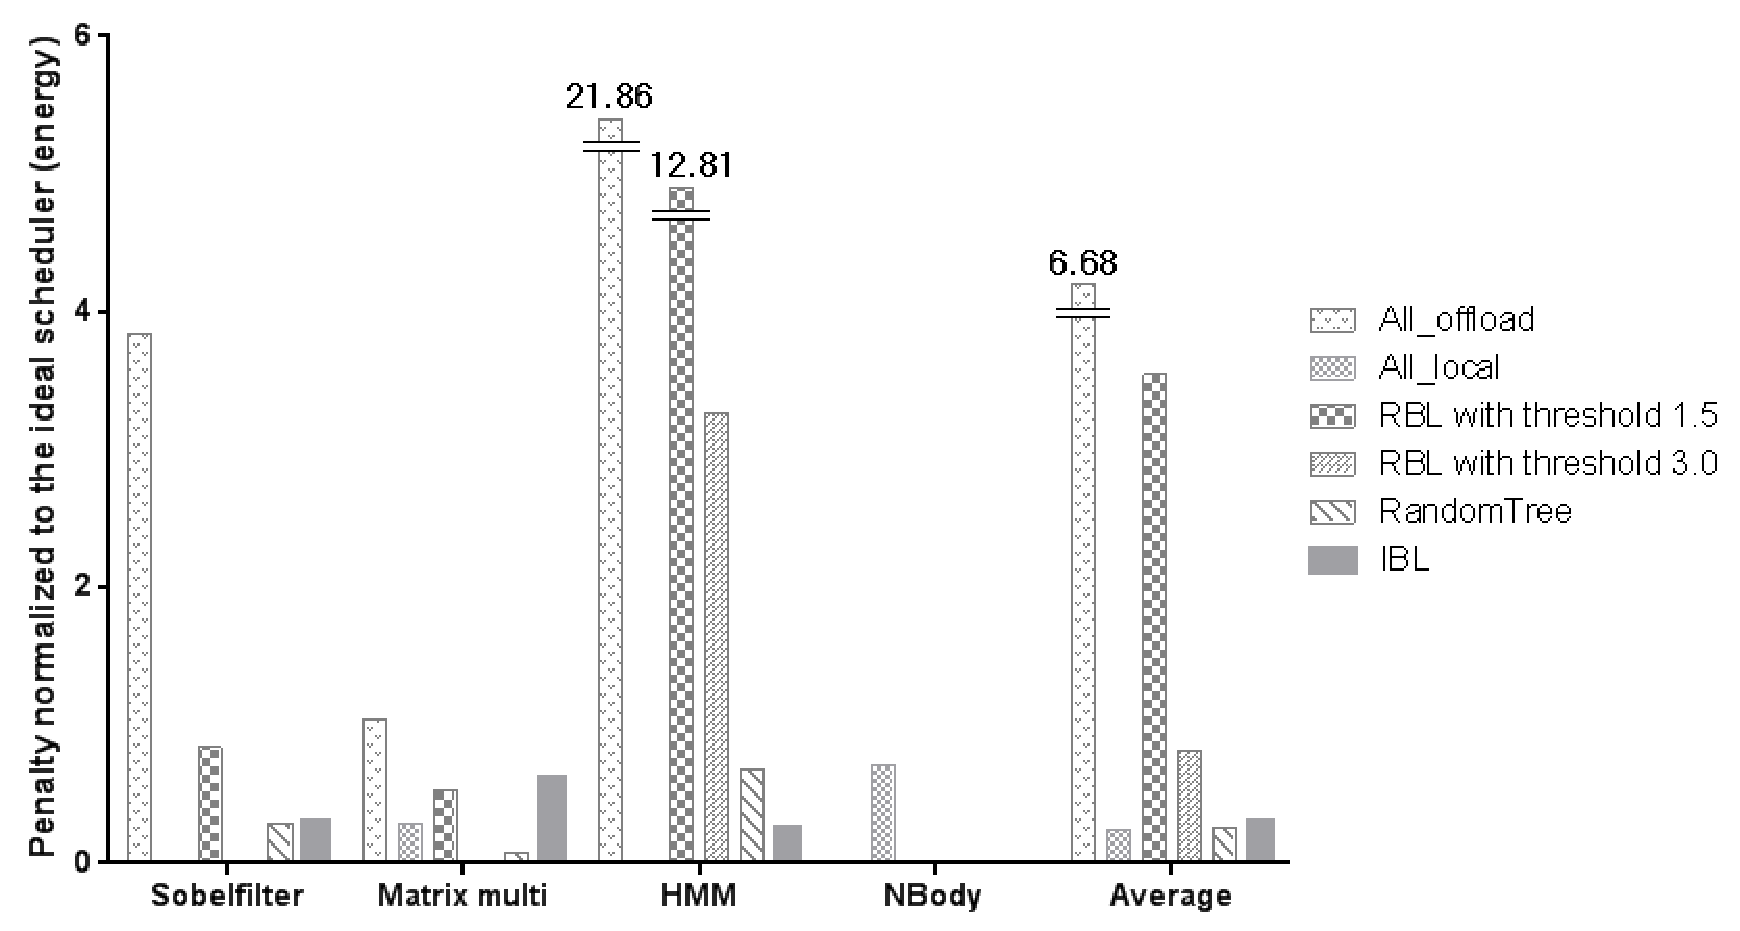
\epsfig{file=figs/penalty_energy.eps, width=5.5in}
\caption{Penalty(energy consumption) normalized to the oracle scheduler}
\label{fig:penalty_energy}
\end{figure}
%
\begin{equation}
\begin{split}
	penalty_{normalized} \\ 
		&	= (execution\_time_{ML} 
               - execution\_time_{oracle}) \\
        &        / execution\_time_{oracle}
\end{split}
\label{equ:penalty}
\end{equation}
%
where {\it execution\_time$_{ML}$} and 
{\it execution\_time$_{oracle}$} are the processing times 
of the workload scheduled by the machine learning-based scheduler 
and the oracle scheduler, respectively.
%
For the penalty in terms of energy consumption, 
{\it execution\_time$_{ML}$} and {\it execution\_time$_{oracle}$}
should be replaced with the mobile device's energy consumption to 
execute or offload the workload scheduled by each scheduler.
%
In this evaluation, the penalty implies the extra costs that the mobile
device or user has to pay additionally over the oracle scheduler when
the machine learning-based scheduler makes a wrong decision. 
%
To profile energy consumption of the mobile device, I used
PowerTutor~\cite{powertutor} which is an application for the variants of
Android devices that displays the power consumed by major components
such as CPU, network interface, LCD display, and GPS receiver.\\
%
As you can see, the Instance-Based Learning scheduler has the smallest
penalty in terms of the execution time because it has the highest
scheduling accuracy.
%
For energy consumption, moreover, the Instance-Based Learning scheduler has
a fairly small penalty compared with Rule-Based Learning scheduler.
%  
Note that, for sobelfilter, the penalty in terms of both the execution
time and energy consumption is lower than other execution kernels,
because the gap of the execution time and energy consumption for
sobelfilter between offloading and the local execution is relatively
small.
%
Therefore, the penalty for sobelfilter is less significant than the
cases of other execution kernels when the scheduler makes a wrong
decision on offloading or the local execution.
%

\section{Online Runtime Scheduler}
\label{scheduler:online}
%
In the previous section, I demonstrated the offline runtime offloading
scheduler based on various machine learning algorithms by illustrating
the scheduling accuracy and the penalty with regard to the execution
time and energy consumption of the mobile platforms.
%
In this section, I explore the potential possibility and benefits of an
online runtime scheduler for mobile offloading framework in which
the online scheduler can be trained through the previous experiences
automatically and adapt to the dynamic situation.
%
\subsection{Implementation of the Online Offloading Scheduler}
\label{scheduler:online_impl}
%
I first implemented the prototype of the online runtime scheduler
based on the Instance-Based Learning algorithm for the mobile offloading
framework.
%
The reason why I chose the Instance-Based Learning algorithm for the
online runtime scheduler is due to the simplicity of the algorithm and
the ability to quickly apply newly seen data to its future decisions.
%
Usually, other machine learning algorithms such as neural networks or
linear regression have its own the classification model and it is
required to be completely modified when a new instance data is added to
the training dataset.
%
However, Instance-Based Learning simply stores the new instance to the
training dataset, and the new instance is used to predict a next coming
problem instance along with previous stored instances.
%
In addition to its simplicity, in the evaluation for the offline offloading scheduler,
Instance-Based Learning showed the best performance among various
machine learning algorithms I used for the evaluation.\\
%
The following is the scheduling process of our prototype of the online
scheduler.
%
Once the application starts, the online scheduler executes the
application locally at once to figure out the information which is
required for profiling the workload such as the local execution time, the
size of data, or the number of the invocations for argument setup.
%
Then, the scheduler enters the training phase by unconditionally
offloading the execution to the remote server {\it N} times, and
each case is labeled according to the performance comparison between
offloading and the local execution.
%
The labeled instance is stored into the training database.
%
For the prototype, I set {\it N} with 16.
%
After the training phase, the scheduler starts the scheduling process by
measuring the Euclidean distance between a new scheduling problem and
the instances stored in the training database.
%
When offloading is scheduled, the scheduler offloads the workload and 
measures the execution time for offloading.
%
If offloading takes shorter than the local execution, then that instance
is added to the training database as {\it offload}.
%
On the other hand, it is stored as {\it local}.\\
%
To update the training database, the scheduler keeps adding the
new instance to the database without removing any previous stored
instance until the database is full.
%
Only if the database is full, the oldest instance will be replaced with
the new one.
%
For the implementation, I try to find the optimal number of instances for
the database which covers as many cases as possible, but takes reasonably small 
memory space (less than 1MB) and time (less than 0.01sec) to schedule a
new problem.
%
I chose 5,000 instances database which requires only 0.1MB of memory.
%
This memory usage occupies only less than 0.0007\% of typical memory
sizes of
contemporary mobile devices (e.g 16GB or 32GB).
%
Also, even though it takes 5$\sim$6msec to measure the Euclidean
distance of the new scheduling problem with 5,000
instances, I believe that instance generalization or clustering techniques for
the database such as~\cite{domingos, chang} can help the
scheduler significantly reduce the measurement time. 
%

\subsection{Evaluation for the Online Offloading Scheduler}
\label{scheduler:online_eval}
%
\begin{figure}
\centering
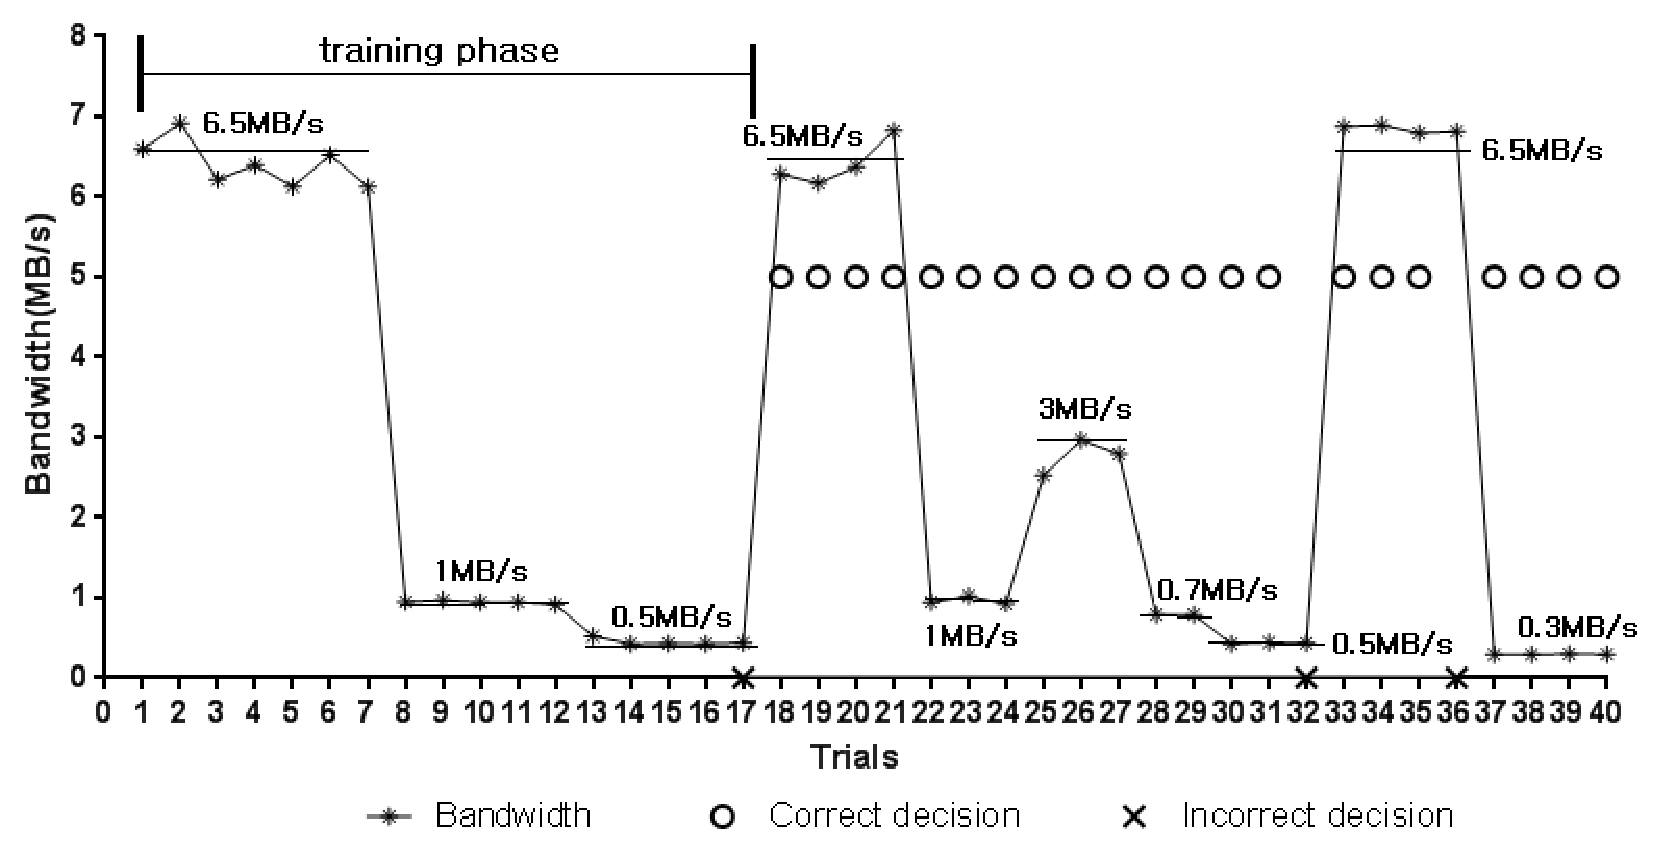
\epsfig{file=figs/online.eps, width=5.5in}
\caption{Adaptability of the online scheduler against dynamic network
conditions}
\label{fig:online}
\end{figure}

%
In order to evaluate the prototype of our online scheduler, I conducted
an experiment in which I change network conditions and observe how
well the scheduler learns and adapts to dynamic network conditions.
%
In this experiment, the client and the remote server are directly
connected through a wireless router and I controlled the network
bandwidth between them using TC.
%
Also, I used sobelfilter for the offloaded execution kernel.
%
Figure~\ref{fig:online} shows the ability to adapt the online scheduler to dynamic
network conditions.\\
%
\indent During the training phase, I setup different network conditions where
the scheduler is trained with three network bandwidths: 6.5MB/s, 1MB/s,
and 0.5MB/s.
%
After the training phase, the scheduler makes a decision on offloading
or the local execution in six different network bandwidths as shown in
Figure~\ref{fig:online}.
%
As you can observe, the scheduler makes the correct decisions in dynamic
network conditions except for 17th, 32nd, and 36th trial.
%
These incorrect decisions are because network bandwidth is changed
after the scheduler makes a decision.
%
As a result, the actual cost for data transfer is different with what
the scheduler predicts. 
%
Furthermore, even at the unseen conditions in the training phase such as
3MB/s or 0.3MB/s, the scheduler works correctly by making right
decisions.
%
Consequently, I observed the possibility and the potential benefits of
machine learning-based online offloading scheduler in this experiment. 
%
\section{Summary}
\label{scheduler:summary}
%
In this section, I proposed machine learning-based runtime scheduler for
mobile offloading framework.
%
Before addressing the scheduling problem of the mobile offloading
framework, I performed detailed measurement experiments under various
network conditions and mobile applications to show the necessity and
efficacy of an adaptive offloading mechanism.\\
%
In order to examine the feasibility of applying machine learning
techniques to the adaptive scheduling problem, I utilized Weka which is
a Java-based open source package.
%
To this end, I used computation to communication ratio, which represents
the local processing time for the workload, the amount of data transfer,
and network bandwidth, as an attribute of the machine learning
technique.
%
After investigating the scheduling accuracy of several machine learning
algorithms using Weka, I choose a few machine learning algorithms which
have relatively high scheduling accuracy to implement an offline
offloading scheduler.
%
In the evaluation, I showed that although Instance-Based Learning 
offloading scheduler is fairly simple and has low overhead, it provides
performance advantages over non-adaptive scheduling policy or even
another machine learning algorithm-based schedulers such as RandomTree
or Rule-Based Learning.
%
In fact, the scheduler based on Instance-Based Learning
performed 7\% better than RandomTree and 3\% better than Rule-Based
Learning.\\
%
Furthermore, by taking the complexity and scheduling performance into
account, I selected Instance-Based Learning algorithm for an online
scheduler for mobile offloading framework.
%
Using Instance-Based Learning online scheduler, I demonstrated
the potential benefits and the ability of the online offloading
scheduler to adapt into dynamic network conditions.
%

\chapter{ONLINE TRAINING FOR MOBILE OFFLOADING SCHEDULER}
\label{chap:online}
As I validated through detailed measurement experiments in Chapter V,
one important fact is that benefits and drawbacks from offloading
computation-intensive portions of mobile applications can be influences
by various internal and external factors, such as application
requirements, network conditions, and computing capabilities of mobile
and external devices.
%
Accordingly, \textit{whether to offload or execute locally} needs to be
decided dynamically based on internal and external conditions, and
monitoring the aforementioned dynamic features at runtime is required to
make offloading decisions.
%
Otherwise, incorrect offloading decisions may cause performance
degradation and/or increase energy consumption.
%
Related work has also considered dynamic scheduling for mobile
offloading frameworks.
%
For example, Kwon et al.~\cite{kwon} consider a simple threshold-based
scheduler in which the framework decides to offload  mobile
computations only when the data transfer size is higher than a certain
threshold.
%
MAUI~\cite{maui} utilizes a linear regression model using predefined
features, such as workload, network and device characteristics, to make
offloading decisions.\\
%
Even though these systems consider runtime schedulers for mobile
offloading, which take dynamic features such as data transfer size or
network conditions into account to make offloading decisions, it is
impractical for these approaches to build a generic offloading decision
policy embracing all possible cases over dynamic mobile environments.
%
For instance, consider that a mobile user walks around a shopping complex, while
receiving offloading-capable mobile services such as gaming or
augmented reality.
%
In this situation, network latency, bandwidth and availability can be changed from
moment to moment.
%
In addition, according to network conditions, the offloading service may
trigger the service migration to other remote servers, which may have
different computing power capabilities, to deliver better service experience
to the mobile user.
%
However, it is infeasible to define a static scheduling model by
expecting various network conditions and computing capabilities of remote
offloading servers.  
%
Furthermore, the scheduling policy, which is fitted with a particular
application, may not work correctly for other applications due to
different application requirements and characteristics.
%
For example, gaming and image processing applications may have different
computation complexity, though they process a similar size of data.\\
%
In this Chapter, I aim to develop a novel framework for an
adaptive runtime scheduler for mobile offloading by employing online
machine learning techniques -- MALMOS (machine learning-based mobile
offloading scheduler).
%
In this approach, a machine learning classifier makes decisions of
whether mobile computations should be offloaded to external resources,
or executed locally. 
%
To this end, I extend our work on offline machine
learning-based runtime scheduler~\cite{ml}, and develop a novel online
scheduling module in which any appropriate machine learning classifier
can be utilized for the runtime offloading scheduler.
%
Furthermore, MALMOS provides an online training mechanism for
the machine learning-based runtime scheduler such that it supports a
policy that dynamically adapts scheduling decisions at runtime based
upon the observation of previous offloading decisions and their
correctness.\\
%
To demonstrate its practical applicability, I integrated MALMOS
with an existing Java-based, offloading-capable code refactoring
framework, \textit{DPartner}~\cite{dpartner}.
%
Originally, the offloading-capable mobile applications generated by
DPartner depend on static (or user-provided) input to decide whether to
execute offloadable computations (i.e. Java classes) locally or remotely.
%
By combining the machine learning-based runtime scheduler with
these applications, offloading decisions are dynamic and do not require
any user input.
%
I have implemented an online-scheduled DPartner prototype, and used it
to perform quantitative experiments with Android mobile devices and
applications to evaluate the performance and cost for three machine
learning algorithms: instance-based learning, single layer perceptron, and na\"{i}ve
Bayes, with respect to classifier training time, classification time,
and scheduling accuracy.
%
Particularly, I examined the adaptability of MALMOS to various network
configurations and computing capabilities of remote resources by comparing
the scheduling accuracy with two static scheduling cases:
threshold-based and linear equation-based scheduling policies.
%
Even though there have been prior related studies which suggest
utilizing machine learning techniques for mobile computing environments,
to the best of our knowledge, our work is the first to consider an
online training mechanism for the machine learning-based runtime
scheduler, and to demonstrate with a end-to-end system performance and
cost of various machine learning algorithms for the runtime scheduler of
mobile offloading tasks.\\
%

\section{Background and Challenges}
\label{online:challenges}
%
In this section, I summarize our work on offline-trained
machine learning-based runtime scheduler for mobile offloading
framework.
%
Then, I describe challenges on the online training mechanism for the
machine learning-based runtime scheduler.
%

\subsection{Offloading Performance}
\label{online:performance}
In the previous Chapter, I studied a runtime scheduler for
mobile offloading framework through detailed measurement experiments.
%
With an OpenCL-based mobile offloading framework~\cite{ocloff}, I
performed various experiments using four different OpenCL workload
kernels used in a variety of areas such as image processing and
simulations.
%
Also, in order to observe the impact of different network conditions on
the offloading performance, I configured different network conditions:
local area network, campus network, and wide area network (i.e. Amazon
EC2 cloud).
%
In the evaluation, I verified that different network conditions result
in significant differences in offloading performance.
%
Also, each OpenCL workload kernel shows different offloading
performance, even though they process similar size of data, because each
kernel has different computational complexity.
%
These results demonstrated offloading performance
variation over different network conditions and OpenCL workload
kernels.\\
%
Based on our observation, I applied machine learning techniques
to runtime scheduling.
%
I trained various machine learning classifiers with
\textit{Weka}.
%
Then, I implemented a machine learning-based runtime scheduler by
building the trained machine learning classifiers onto the
OpenCL-based mobile offloading system.
%
In our evaluation, I observed that most of the machine learning-based
schedulers show scheduling accuracy higher than 80\%.
%

\subsection{Offline vs. Online Training}
\label{online:training}
There exist two possible ways to train the machine learning
classifier: \textit{offline} and \textit{online} training.
%
In offline training, the machine learning classifier can be trained
using a set of pre-collected static data.
%
Once the machine learning classifier is trained in the initial training
phase, the classifier does not change its prediction behavior.
%
It is therefore difficult to reflect unseen situations or conditions
which have not been trained in the initial training phase.
%
For that reason, offline machine learning should be trained through a
large set of data which covers as many cases as possible in order to
accomplish high prediction performance.\\
%
On the other hand, the online machine learning technique does
not depend on any pre-trained classifiers to predict the future
behaviors of the target system.
%
Instead, the online machine learning techniques trains its classifier
when a new data instance is available at runtime.
%
More specifically, the classifier of the online machine learning
technique is trained whenever the comparison result between the
prediction value and actual behavior is available.
%
Thus, the main challenge of online machine learning is to deliver the
prediction correctness into the training process, so that it can train
the classifier continuously based upon the prediction correctness feedback.
%
However, it can be too expensive to determine the correct prediction,
since the scheduler may have to attempt all of the possible decision
cases to know which prediction is correct.\\
%
In this Chapter, I extend our work on the offline
machine learning-based mobile offloading scheduler by considering an
adaptive online training mechanism.
%
In the case for the mobile offloading scheduler, even though
there exist only two possible cases (offloading and local processing),
the mobile platform still has to pay for both offloading and local
processing.  
%
Therefore, it is important to minimize the training cost while
guaranteeing reasonably acceptable scheduling performance.
%
This work addresses this challenge by proposing the adaptive online training
mechanism in which the training phase can be dynamically stretched and
shrunk according to the scheduling performance so that the mobile device
does not have to pay the unnecessary training cost by retaining a static
length of the training phase. 
%

\section{Architecture of MALMOS}
\label{online:architecture}
In this section, I describe the architecture and main modules of MALMOS.
%
Then, I describe implementation details on MALMOS with the adaptive
online training mechanism.
%
Lastly, I explain how MALMOS can be integrated with mobile offloading
frameworks, using DPartner as a concrete scenario.
%
The overall architecture and main modules of MALMOS are illustrated in
Figure~\ref{fig:malmos}.
%
The dotted lines indicate the application and network features flow path, and the
solid lines are the application computing tasks or scheduling-related
commands flow path.
%
\begin{figure}
\centering
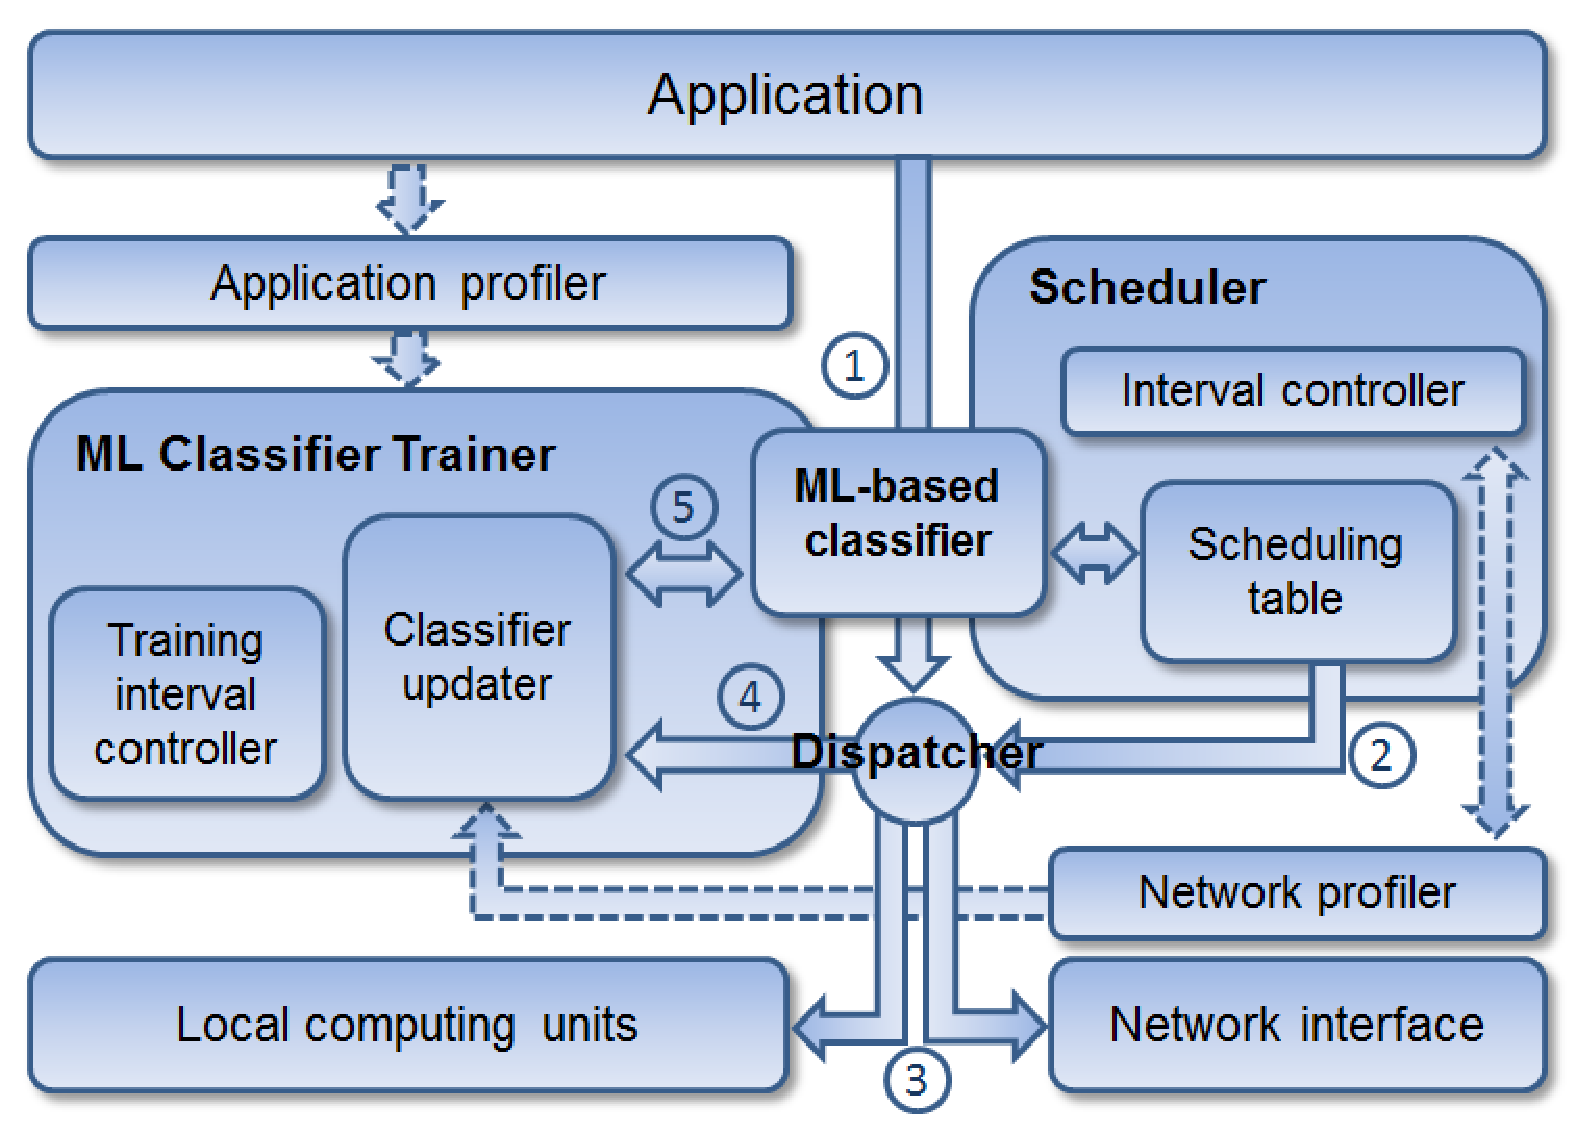
\epsfig{file=figs/malmos.eps, width=4.0in}
\caption{Overall architecture of MALMOS with online training}
\label{fig:malmos}
\end{figure}
%

\subsection{Architecture and Modules of MALMOS}
\label{online:module}
As depicted in Figure~\ref{fig:malmos}, the overall architecture consists
of four main modules: computation dispatcher, runtime scheduler, machine
learning classifier, and the trainer for the machine learning classifier.
%
These four main modules interact with each other to schedule and
execute offloadable tasks, and to train the machine learning
classifier. 
%
At runtime, MALMOS operates alternatively in either of two different phases:
\textit{runtime scheduling phase} and \textit{online training phase}.
%
In the runtime scheduling phase, tasks are executed locally or remotely
based on the decisions from the scheduler.
%
First, the computation dispatcher receives an offloadable task
(\textcircled{1}).
%
%In the runtime scheduling phase, first, the computation dispatcher
%receives an offloadable computation (\textcircled{1}).
%
Then, according to the decision provided by the scheduler module
(\textcircled{2}), the dispatcher forwards this task to the appropriate
execution unit (\textcircled{3}): \textit{either} a local computing unit, or a
remote computing resource (through the network interface).\\
%
In contrast, in the online training phase, the machine
learning classifier is trained in accordance with the scheduling
performance (i.e. scheduling accuracy). 
%
In order to determine the scheduling performance, the offloadable
computation task is forwarded to and executed in \textit{both} execution
units; the computation dispatcher records both execution times, and
feeds back the performance comparison to the classifier trainer
({\textcircled{4}).
%
Based on this feedback from the dispatcher, the classifier trainer updates
the machine learning classifier ({\textcircled{5}).
%
The implementation details for these modules are as follows:\\
%
\textbf{Computation dispatcher.} This module has the
responsibility to dispatch and forward offloadable computation tasks to
the appropriate computing unit: remote computing resource (for offloading) or
local processing units (for local execution) according to the scheduling
decision from the scheduler module stored in the scheduling table.
%
In the online training phase, however, the computation dispatcher works
differently by forwarding and executing computation tasks in both local
processing units and remote computing resources.
%
Also, this module provides feedback to the classifier update in the
machine learning classifier trainer module, by comparing the performance
between offloading and local processing and feeding back which execution
leads to better performance.\\
%
\textbf{Machine learning classifier.} The machine learning classifier is
in charge of making decisions on offloading or local processing for
offloadable tasks.
%
The main difference, which distinguishes MALMOS from the previous
approaches on mobile offloading schedulers, is that it does not rely on
any predefined scheduling policies.
%
Instead, the machine learning classifier hooks up to the classifier
trainer, so the trainer updates the classifier at runtime whenever the feedback from
the computation dispatcher is available, and the machine learning
classifier adapts its decision behavior with changes of internal and
external environments.
%
When the scheduler module sends the request for offloading decisions
with the attributes obtained by the network and application profiler,
the machine learning classifier makes the decisions and stores them into
the scheduling table in the scheduler module.
%
Even though it is possible to adopt various attributes
from internal (application) and external (network, remote resources)
environments, for the current implementation, I employ two attributes:
the size of data to be sent to the remote resource, and the network
bandwidth.\\
%
\textbf{Runtime scheduler.} This module schedules the offloadable
computation tasks by sending the decision requests with the capture of
internal and external dynamic features.
%
Then, it stores the decision results from the classifier to the
scheduling table so that the computation dispatcher can forward each
computation tasks to the appropriate computing unit through looking up
the scheduling table.
%
Scheduling the computation tasks requires to profile internal
and external dynamic features, such as data size of inputs to the tasks
and network conditions. 
%
I achieved this profiling by implementing application and network
profilers.
%
For the application profiler, I defined an application programming
interface (API) to monitor the invocation of the offloadable computation
tasks and capture the size of input arguments.
%
Also, for the network profiler, I implemented network bandwidth
measurement by simply dividing the size of a probing packet with the elapsed
time to send the probing packet as described in~\cite{nws}.\\
%
However, profiling application and network conditions incurs
additional cost in terms of runtime overhead and energy consumption,
which means that too frequent profiling may lead to high overhead.
%
For this reason, I consider two scheduling strategies.
%
In the first strategy, each time offloadable tasks are invoked from the
mobile application, the runtime scheduler requests to make offloading
decisions while profiling application and network conditions.
%
I refer to this strategy as \textit{on-demand scheduling}.
%
Another strategy is \textit{periodic scheduling}, in which the
scheduler makes the decision requests asynchronously with actual
invocations of offloadable tasks, but periodically with a certain
interval.
%
Therefore, each profiler does not need to inspect application
and network conditions for every invocation of the offloadable tasks.
%
Also, in the periodic scheduling strategy, the scheduling interval
can increase and decrease dynamically according to network behavior
in order to obtain more up-to-date network conditions.
%
If the variation of network bandwidth is less than a threshold, which
can be thought as a steady-state network status, the scheduling interval 
becomes longer (e.g. twice as current interval).
%
The assumption is that it is likely that former scheduling can be 
still effective for the near future.
%
In contrast, if the variation of network bandwidth is greater than the
threshold, the interval becomes half of the current interval, leading to
more frequent scheduling.\\
%
\textbf{Machine learning classifier trainer.} With the feedback on the
performance comparison between offloading and local processing from the
computation dispatcher, the machine learning classifier trainer updates
the machine learning classifier.
%
In order to compare the performance between offloading and local
processing, the trainer creates one separate thread for local
processing, so that offloading and local processing can be executed
concurrently.
%
Then, the computation dispatcher measures the execution time for both
offloading and local processing to compare the performance and provides
the comparison result to the classifier updater. 
%
Finally, the classifier updater trains the machine learning classifier 
with the feedback from the computation dispatcher and the attributes
from the profilers.
%
\begin{figure}
\centering
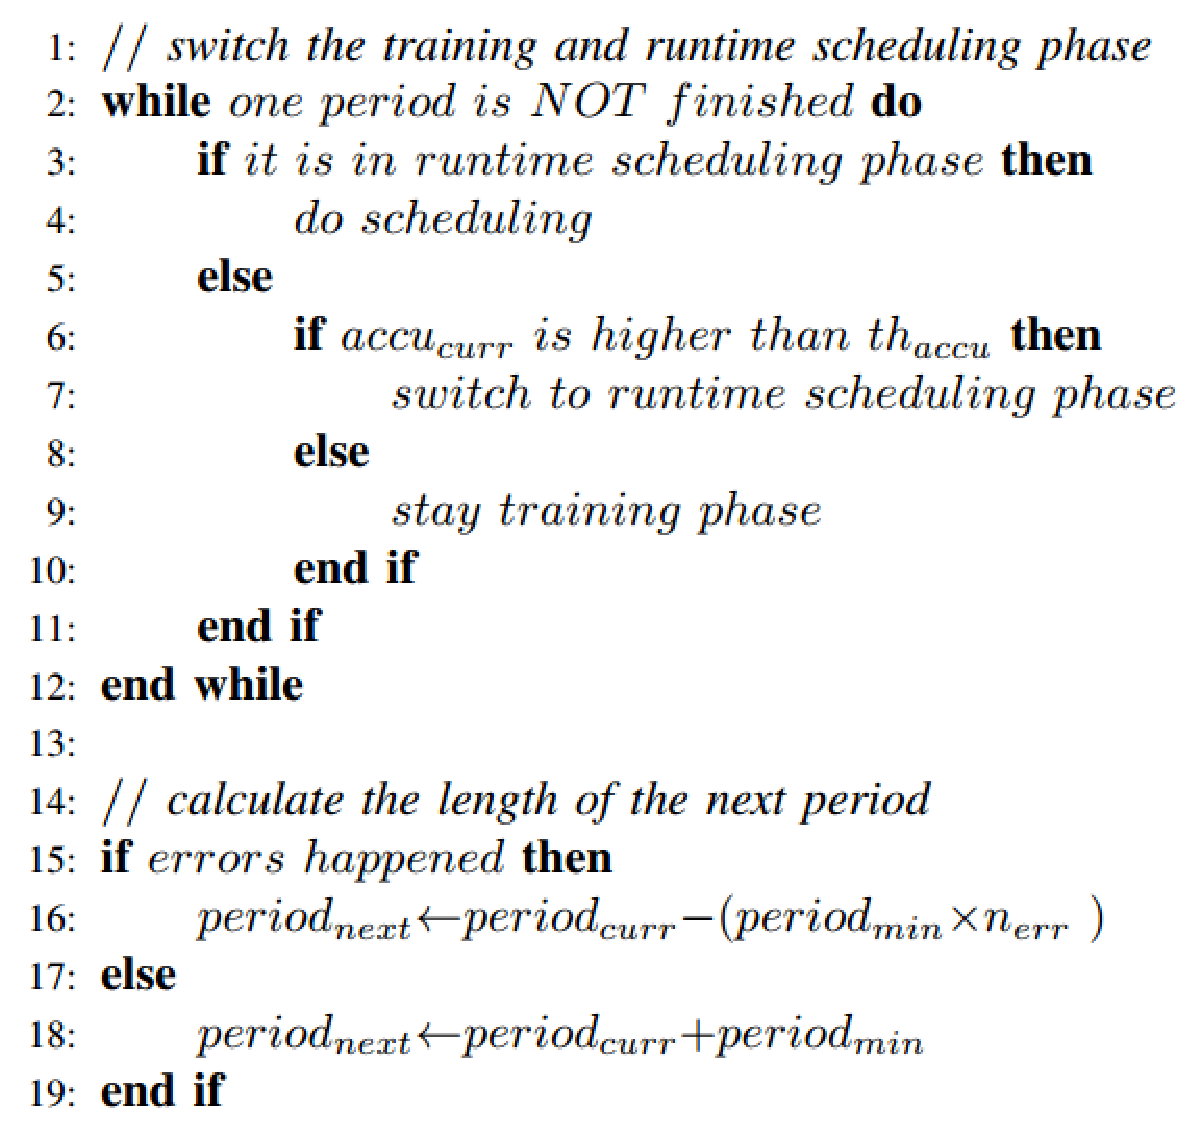
\epsfig{file=figs/malmos_algorithm.eps, width=4.0in}
\caption{Pseudo-code for adaptive online training mechanism}
\label{fig:malmos_algorithm}
\end{figure}
%

\subsection{Adaptive Online Training Mechanism}
\label{online:module}
One of the main contributions of this work is an adaptive online
training mechanism which allows the training phase duration to stretch
and shrink dynamically according to the scheduling accuracy.
%
The pseudo-code of the adaptive online training mechanism is shown in
Figure~\ref{fig:malmos_algorithm}.
%
First, lines 2--12 decide to switch the online training and runtime
scheduling phase by calculating the current scheduling accuracy.
%
In the training phase, if the current accuracy ($accu_{curr}$) is higher
than the accuracy threshold ($th_{accu}$), the online training mechanism
switches to the runtime scheduling phase.
%
Otherwise, it stays in the training phase.
%
Next, the length of the next period is calculated according to the
number of incorrect decisions (lines 15--19).\\
%
Figure~\ref{fig:malmos_example} illustrates an example of how the adaptive online
training mechanism works.
%
In this example, I set the accuracy threshold ($th_{accu}$) to 70\% and
the minimum length of one period to 5 to make the explanation clear to
understand at a glance.
%
Also, I assume that there is no incorrect decision or scheduling error
in the first, second, and fourth period, but one error in the third
period.
%
In order to measure the current scheduling accuracy ($accu_{curr}$) of
the classifier, the trainer observes whether the performance comparison
matches with the offloading decision.
%
For example, if the classifier makes a decision to offload and
offloading actually has better performance than local processing, I
regard this case as a correct decision.
%
Then, I calculate the current scheduling accuracy using
Equation~\eqref{equ:accuracy}.
%
\begin{figure}
\centering
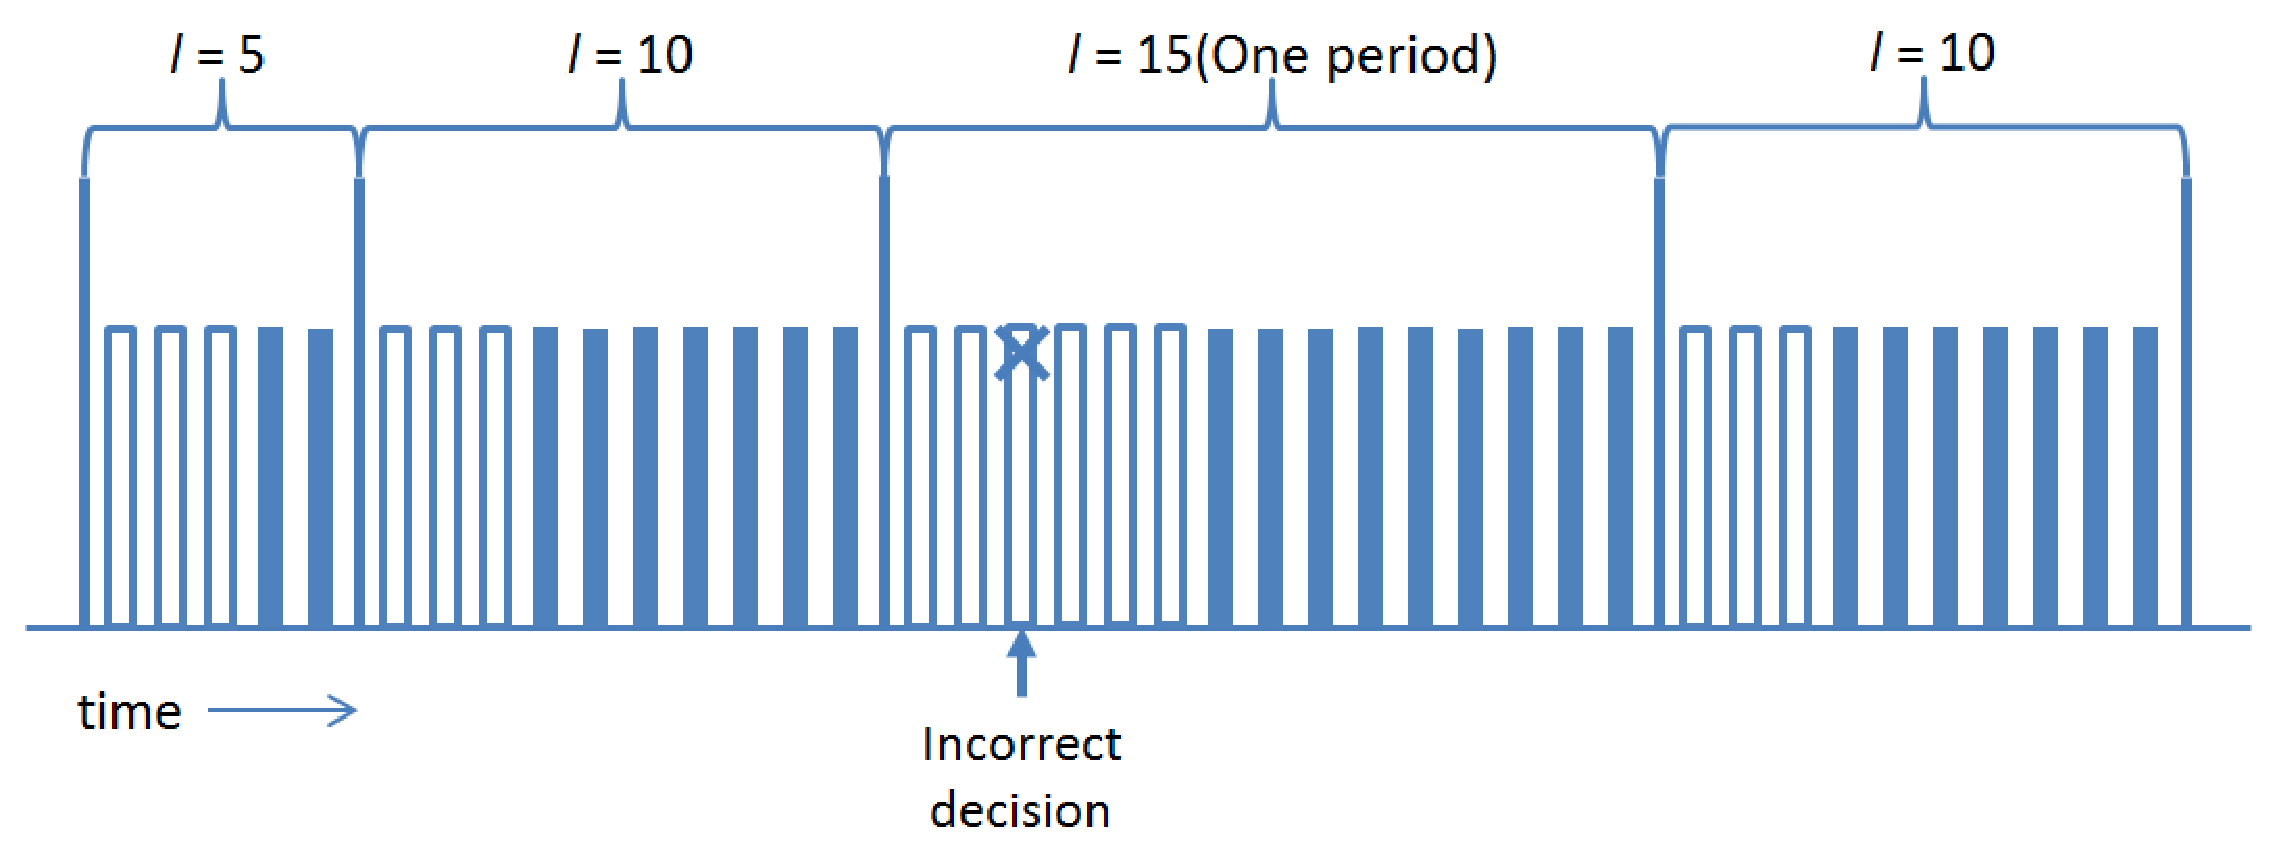
\epsfig{file=figs/malmos_example.eps, width=4.5in}
\caption{An example of the adaptive online training mechanism}
\label{fig:malmos_example}
\end{figure}
%
\begin{equation}
	accu_{curr} = N_{correct}\:/\:(N_{total} + 1)
\label{equ:accuracy}
\end{equation}
%
where $N_{correct}$ and $N_{total}$ are the number of correct decisions
and total decisions.
%
I add one to the denominator in order to avoid 100\% of
scheduling accuracy at just one training (if the decision is correct in
the first training turn, the scheduling accuracy becomes 100\%).\\
%
In Figure~\ref{fig:malmos_example}, the runtime scheduling phase begins after three
training turns in the first and second period because the scheduling
accuracy at third training turn is 75\% which is higher than 
$th_{accu}$, 70\%.
%
Furthermore, because there was no decision error in the first and second
period, the next length of one period increases by adding the
minimum length of one period.
%
Thus, the lengths of the second and third period become 10 and 15,
respectively.
%
In the third period, however, as one incorrect decision has
occurred, the training phase holds for six executions when the
scheduling accuracy becomes higher than 70\%, and the length of the
fourth period decreases by the minimum length of one period multiplied
by the number of incorrect decisions (in this case, 1).
%
This adaptive online training mechanism is inspired by the concept of
the feedback control algorithm used for TCP congestion avoidance called
\textit{Additive Increase Multiplicative Decrease}.
%

\subsection{Integration with On-Demand Java-based Offloading Framework}
\label{online:integration}
To demonstrate the applicability of this approach, I integrated the
modules of MALMOS into the DPartner mobile application framework, which
is capable of automatically refactoring Java-based mobile applications
to identify offloadable computation tasks.
%
Given an Android mobile application, first of all, DPartner examines its
bytecode to classify the Java classes into the anchored and offloadable
classes, so it can be guaranteed that the anchored classes are executed
on the mobile device while directly using a variety of the local sensors
such as the GUI display, camera, accelerator, and GPS.
%
Also, DPartner rewrites the bytecode for the offloadable classes to
implement a special type of the program structure to support on-demand
offloading.
%
Then, DPartner packages the files such as images, xml files, external
libraries, and rewritten bytecode for the offloadable classes, and
generates two separate objects which are deployed into the mobile device
and the remote server, respectively.\\
%
With respect to scheduling, the offloading-capable
Android applications generated by DPartner require either static or
user-provided decisions. 
%
However, static scheduling becomes inaccurate if conditions change, and
it is impractical that the mobile user monitors internal and
external environments and schedules each offloadable mobile computations
at runtime.
%
I address this challenge by integrating MALMOS with the
offloading-capable mobile applications generated by DPartner. 
%
I was able to achieve this integration without requiring deep
modifications or code additions to DPartner.
%
In fact, the only major code addition is to define new APIs to acquire
the data size of offloadable computations and the network bandwidth. 
%
By combining MALMOS with these applications, the mobile user can be free
of the burden of scheduling tasks.
%

\section{Evaluation}
\label{online:evaluation}
In this section, I evaluate the prototype implementation of MALMOS with
respect to the scheduling performance and cost.
%
First, I examine the training and classification time for different
categories of machine learning algorithms: instance-based learning,
single layer perceptron, and na\"{i}ve Bayes.
%
I examined the adaptability of MALMOS to various network conditions and
computing capability of remote resources by comparing the scheduling
accuracy with two static scheduling cases: threshold-based and linear
equation-based scheduling policies, by running three synthetic
applications (hidden Markov model, floating-point matrix multiplication, and
sobelfilter) and two real applications (Linpack and Go game).
%
\subsection{Experimental setup}
\label{online:setup}
Even though high-dimensional machine learning algorithms (such as
decision tree, multi layer perceptron, or support vector machine) can
achieve more accurate scheduling performance, they might be too
expensive to be used for mobile platforms.
%
Based on algorithm complexity considerations, I selected three machine learning
algorithms: instance-based learning, single layer perceptron, and
na\"{i}ve Bayes for out prototype implementation.\\
%
Also, in order to evaluate the adaptability of MALMOS to various
network conditions and computing capabilities of remote computing
resources, I setup experiments using a variety of hardware and
network configurations.
%
First of all, our hardware setup consists of a mobile client and three
different remote servers.
%
I have utilized an Android smartphone, Nexus 5 equipped with 2.3Ghz
quad-core processor and 2GB RAM, and running Android KitKat as the
mobile client.
%
For the remote servers, I used two laptops and one desktop which have
different levels of computing power capabilities.
%
The first laptop has an Intel i5 Quad core 2.6Ghz processor and 8GB RAM, while
the second laptop is equipped with an Intel Core2 Duo 2.0Ghz processor and 2GB
of memory.
%
In addition, I ran CPU-intensive workloads on the second laptop using
\textit{Stress}, a simple workload generator~\cite{stress}, to observe 
the effect of CPU load at the remote resource on the scheduling performance.
%
The third remote resource is a workstation with an Intel Core2 Duo 3.0Ghz processor
and 8GB RAM.
%
All remote servers run Linux OS, Ubuntu 12.04.\\
%
Instead of installing the aforementioned three remote servers in
different network environments, for the network configurations, I
emulated three different network bandwidth characteristics: local area
network, campus network, and wide area network by using the Traffic
Control (TC) tool as described in Table~\ref{table:network_summary}.
%
The experimental setup using TC gives flexibility to vary network
conditions between the mobile device and remote resources.\\
%
I experiment three synthetic applications: hidden Markov
model, floating-point matrix multiplication and sobelfilter, and two real
applications available in Google Play: Linpack~\cite{linpack} and 
Go game~\cite{go}, each having different application requirements 
and computation complexities.
%
For example, sobelfilter is an image edge detection filter; it
takes a relatively large size of input, while its computation complexity
is low.
%
Therefore, I classify sobelfilter as a communication-intensive
application.
%
In contrast, the core computation of Go game is a Monte Carlo
algorithm with iterative random sampling tasks which have high
computation complexity.
%
Thus, Go game is a computation-intensive application.
%
Otherwise, the computation complexity of other three applications
depends on the size of input such as matrix size (for floating-point matrix
multiplication and Linpack), and the number of states (for hidden Markov
model).
%
\begin{figure}
\centering
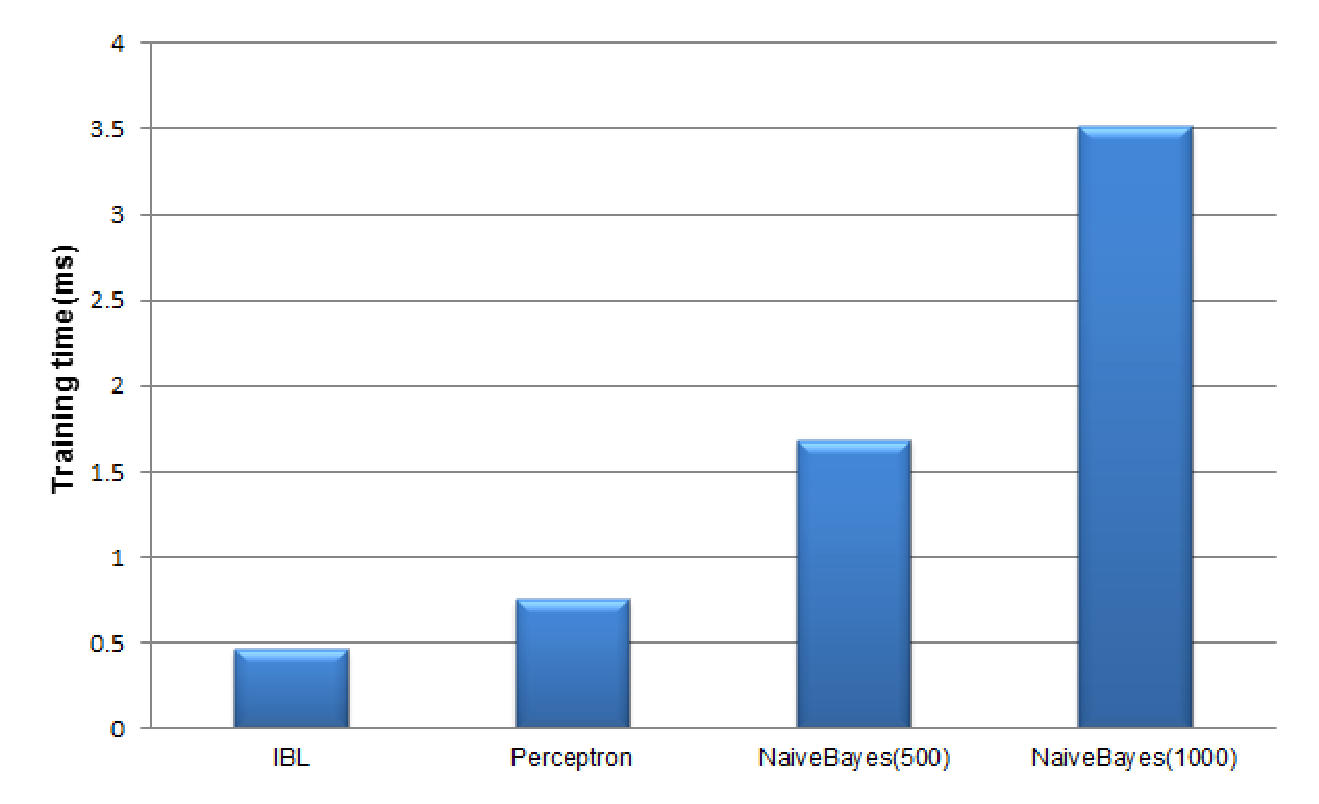
\epsfig{file=figs/training.eps, width=4.5in}
\caption{Training time comparison for three machine learning algorithms}
\label{fig:training}
\end{figure}
%
\begin{figure}
\centering
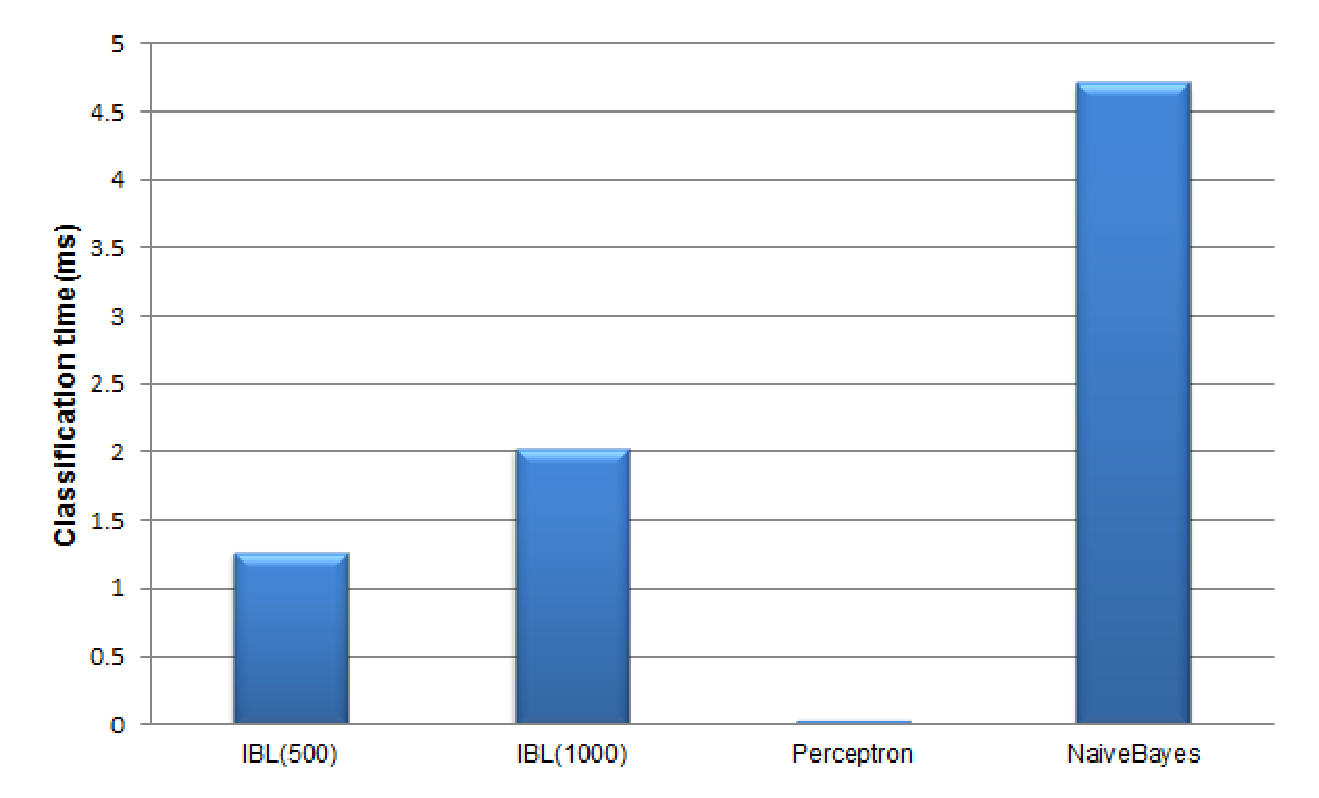
\epsfig{file=figs/classification.eps, width=4.5in}
\caption{Classification time comparison for three machine learning algorithms}
\label{fig:classification}
\end{figure}
%

\subsection{Overhead of training anc classification}
\label{online:overhead}
Since our machine learning-based mobile offloading scheduler keeps
training the classifier, which leads to runtime overhead, I
measured the cost to train the machine learning classifier.
%
As shown in Figure~\ref{fig:training}, instance-based learning has the shortest
classifier training time among three machine learning algorithms.  
%
In fact, the basis for the classification of instance-based learning is
the instance database, where previously experienced cases are stored.
%
Instead of training the explicit classifier, therefore, instance-based
learning adds a new instance to the database for the future
classification, resulting in relatively small training overhead.
%
On the other hand, na\"{i}ve Bayes with 1000 instances of database has
the largest training overhead. 
%
From the algorithm perspective, na\"{i}ve Bayes measures the
probability density for the given classes with the mean and standard
deviation, and chooses the class with the highest probability.
%
Thus, na\"{i}ve Bayes calculates the mean and standard deviation
throughout the previous instances for each class whenever a new instance
is trained.
%
Consequently, na\"{i}ve Bayes with 1000 instances, which requires
relatively heavy calculations for the mean and standard deviation, has
bigger training overhead than other machine learning algorithms.\\
%
Also, Figure~\ref{fig:classification} shows the classification time that the machine
learning classifier consumes to make a decision.
%
Similarly as the training time, na\"{i}ve Bayes shows bigger overhead
than other machine learning algorithms.
%
I used the Gaussian distribution to calculate the probability
density for each class with the mean and standard deviation value.
%
Therefore, the classification for na\"{i}ve Bayes entails complex
arithmetic operations, such as the exponential function and the square
root, which take longer than addition, multiplication, or comparison.
%
For that reason, na\"{i}ve Bayes has the largest classification overhead.
%
Note that perceptron has remarkably low classification overhead compared
with other machine learning algorithms. 
%
For perceptron, the classification process involves calculating the
output from a multivariable linear equation consisting of the attributes
weighted by the coefficients, which requires small amount of
the computation. 
%
As a result, perceptron shows the lowest cost in terms of the
classification time amongst three machine learning algorithms by showing
less than 0.05ms of the classification time.
%

\subsection{Scheduling Accuracy}
\label{online:accuracy}
I then investigated the scheduling accuracy of the three machine learning
algorithms.
%
For an unbiased evaluation, I turned off the adaptive online training
mechanism, and the online training phase and runtime scheduling phase were
uniformly switched in one period (5 of training and 15 of runtime
scheduling).
%
A total of 10 periods were repeated for the average.
%
Also, I demonstrated the adaptability of MALMOS to various network
conditions and computation capability of remote resources by comparing
with two static scheduling policies: threshold-based and linear
equation-based scheduling cases.
%
For the threshold-based scheduler, I empirically observed the
performance for offloading and local processing and picked up the input
size where the execution time of offloading or local processing comes from
behind the other.
%
For instance, if the matrix size is bigger than 170$\times$170,
offloading matrix multiplication to the workstation located in local
area network shows better performance than local processing.
%
As a result, I selected the data size corresponded with 170$\times$170 of matrix
size (i.e. 231KBytes) as the threshold so that when the data size is bigger than the
threshold, the scheduler makes decision to offload the computation.   
%
Therefore, the threshold-based scheduler does not account for the network
conditions.
%
For the case of the linear equation-based scheduling policy, I
established a two dimensional linear equation that distinguishes the
cases where offloading or local processing has better performance than
the other.
%
In order to define this linear equation, I gathered the performance of
offloading each application to the workstation varying the network
bandwidth.
%
In this experimental setup, I measured the scheduling accuracy by
offloading each application to four different remote servers, while
varying the network bandwidth and the size of input.
%
In order to change the network bandwidth, I wrote a simple script file
in which the TC command randomly switches among the three network
bandwidth described in Table~\ref{table:network_summary} in a certain interval during the
experiment.\\
%
\begin{figure}
\centering
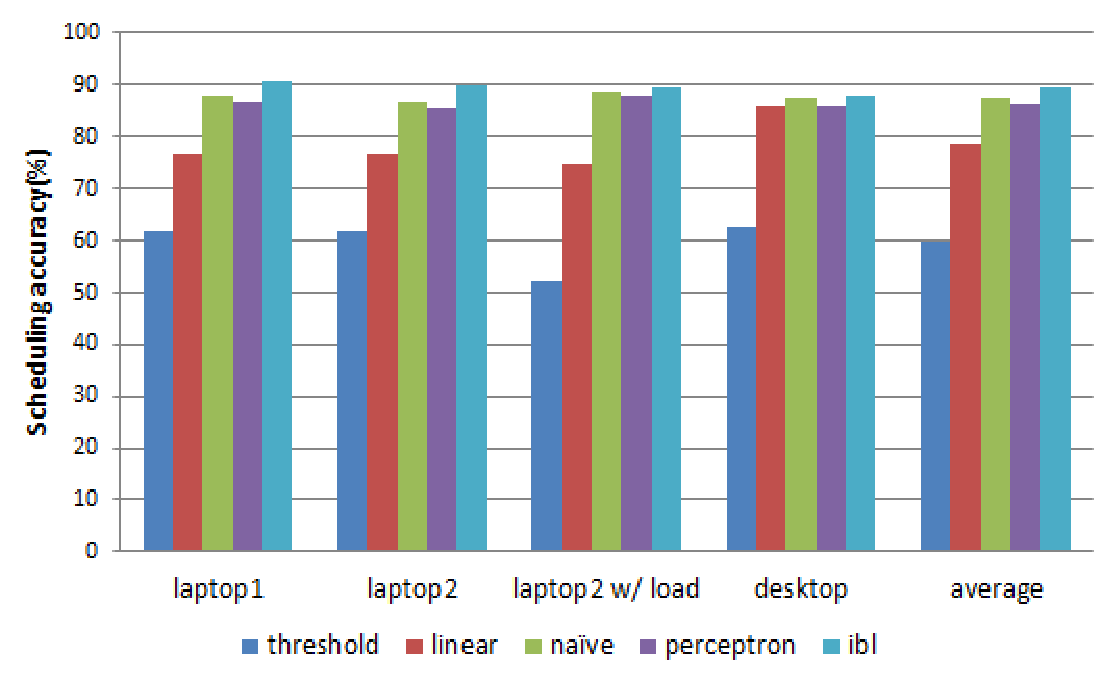
\epsfig{file=figs/scheduling_hmm.eps, width=5.0in}
\caption{Scheduling accuracy for hidden Markov model with various
configurations}
\label{fig:scheduling_hmm}
\end{figure}
%
\begin{figure}
\centering
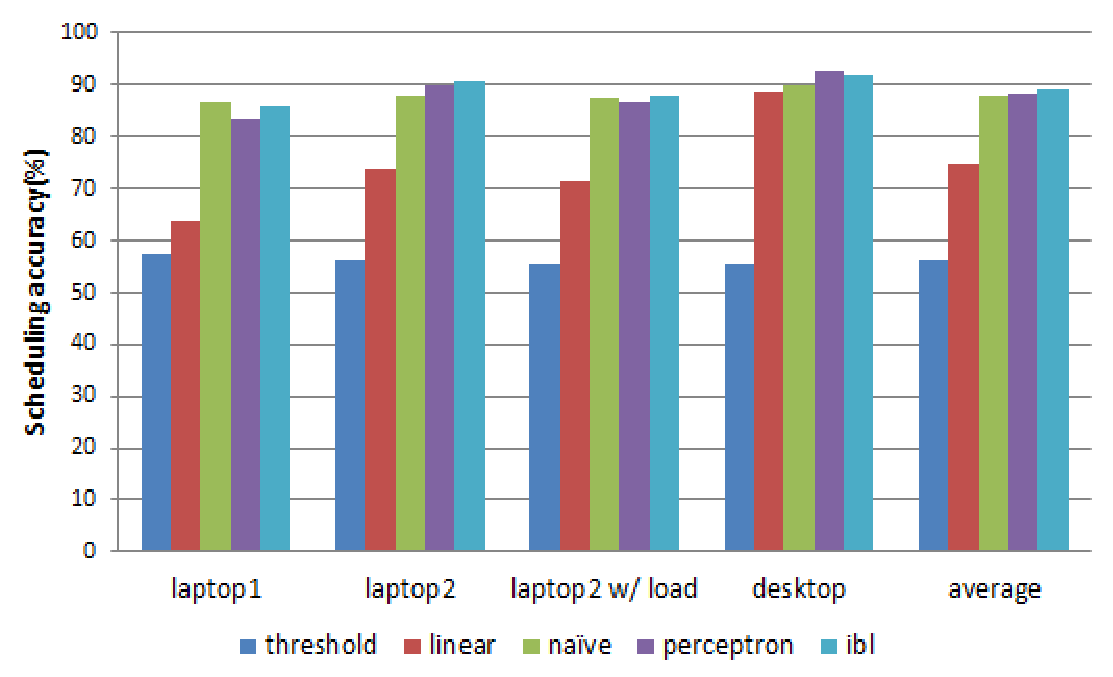
\epsfig{file=figs/scheduling_matrix.eps, width=5.0in}
\caption{Scheduling accuracy for matrix multiplication with various
configurations}
\label{fig:scheduling_matrix}
\end{figure}
%
\begin{figure}
\centering
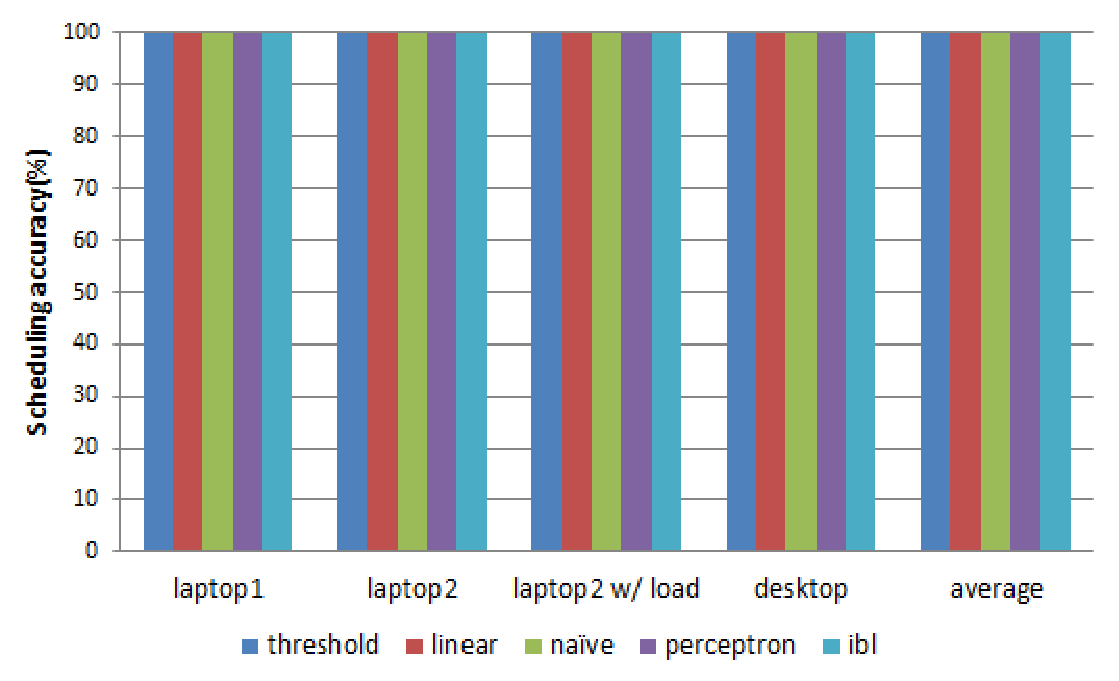
\epsfig{file=figs/scheduling_sobel.eps, width=5.0in}
\caption{Scheduling accuracy for sobelfilter with various
configurations}
\label{fig:scheduling_sobel}
\end{figure}
%
\begin{figure}
\centering
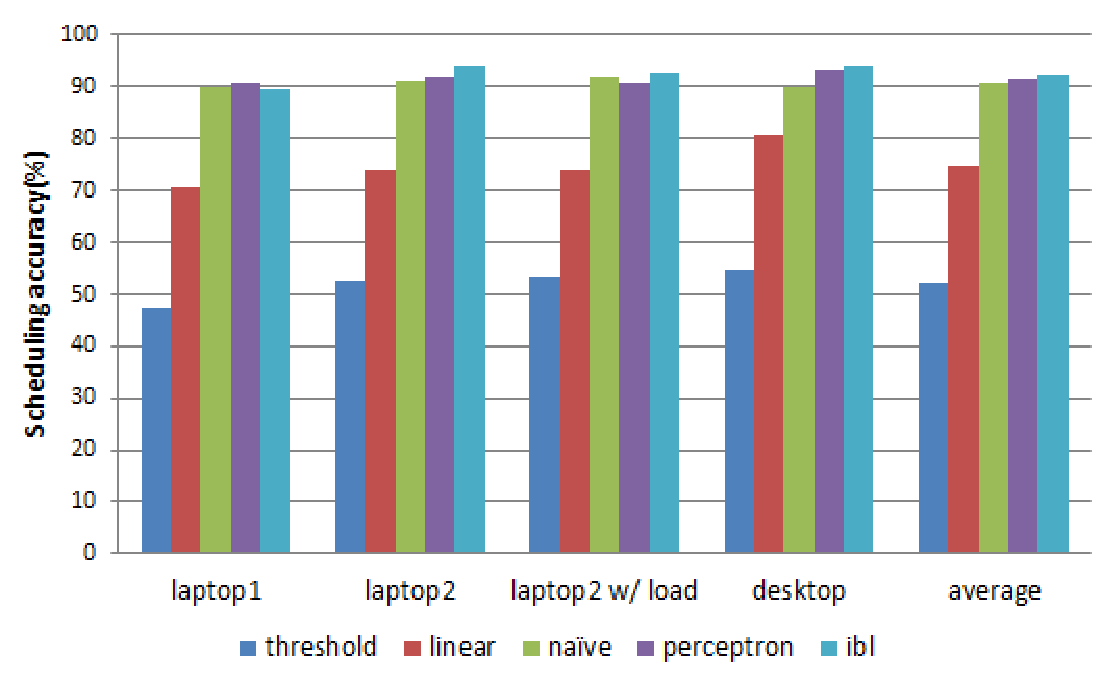
\epsfig{file=figs/scheduling_linpack.eps, width=5.0in}
\caption{Scheduling accuracy for Linpack with various
configurations}
\label{fig:scheduling_linpack}
\end{figure}
%
\begin{figure}
\centering
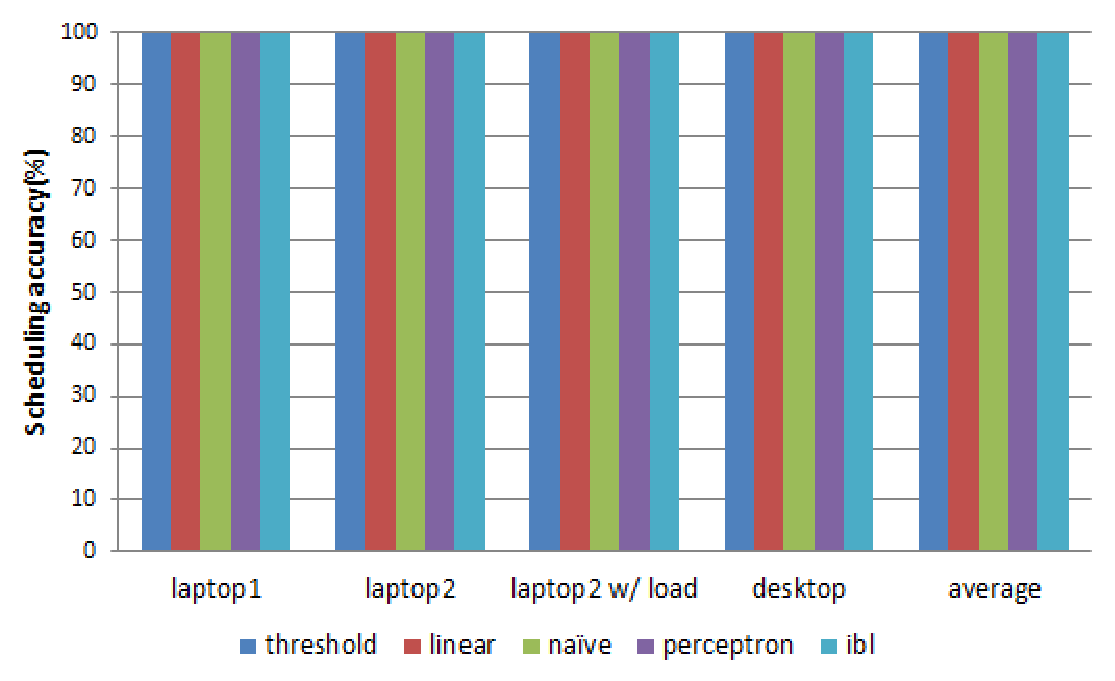
\epsfig{file=figs/scheduling_gogame.eps, width=5.0in}
\caption{Scheduling accuracy for Go game with various
configurations}
\label{fig:scheduling_gogame}
\end{figure}
%
As shown in
Figure~\ref{fig:scheduling_hmm},~\ref{fig:scheduling_matrix},
and~\ref{fig:scheduling_linpack}, MALMOS with
instance-based learning, perceptron, and na\"{i}ve Bayes has better
scheduling performance than the threshold-based and linear
equation-based scheduling policies in the cases of hidden Markov model,
matrix multiplication, and Linpack by showing averagely 86\%$\sim$92.5\% of the
scheduling accuracy over four remote resources setups.
%
The threshold-based scheduler considers only the
size of input data as the decision factor, but does not reflect the
dynamic network bandwidth.
%
Consequently, the threshold-based scheduler shows the poorest scheduling
performance in all experimental scenarios.
%
Particularly, the linear equation-based scheduling policy has similar
performance as three machine learning-based schedulers in the cases of
offloading applications to the workstation, since the linear
equation-based scheduler has been defined based on the offloading
performance with the workstation while varying the network bandwidth.
%
Nevertheless, the linear equation-based scheduler shows poor
scheduling accuracy (ranging from 64\%$\sim$76.6\%) in other remote server
setups, such as laptop or laptop with CPU load.
%
This is because other remote servers have different computing power
capabilities, hence the offloading performance can be quite different
with the case of offloading to the workstation.\\
%
On the other hand, Figure~\ref{fig:scheduling_sobel}
and~\ref{fig:scheduling_gogame} show that all scheduling
cases have exactly 100\% of the scheduling accuracy for sobelfilter and Go game.
%
As I mentioned earlier, sobelfilter and Go game are the
communication-intensive and computation-intensive application,
respectively.
%
For this reason, sobelfilter always prefers local processing and Go game
always prefers offloading.
%
Even in these extremely simple cases, MALMOS demonstrates the scheduling
performance as good as the threshold- and linear equation-based
scheduler.
%
It is worth noting that I established different threshold values and linear
equations for each application. 
%
Even though I used three machine learning algorithms for each
application without any change, MALMOS works universally well in all of
our experimental setup.\\
%
To evaluate end-to-end application performance, I measure the
offloading time of Linpack.
%
\begin{figure}
\centering
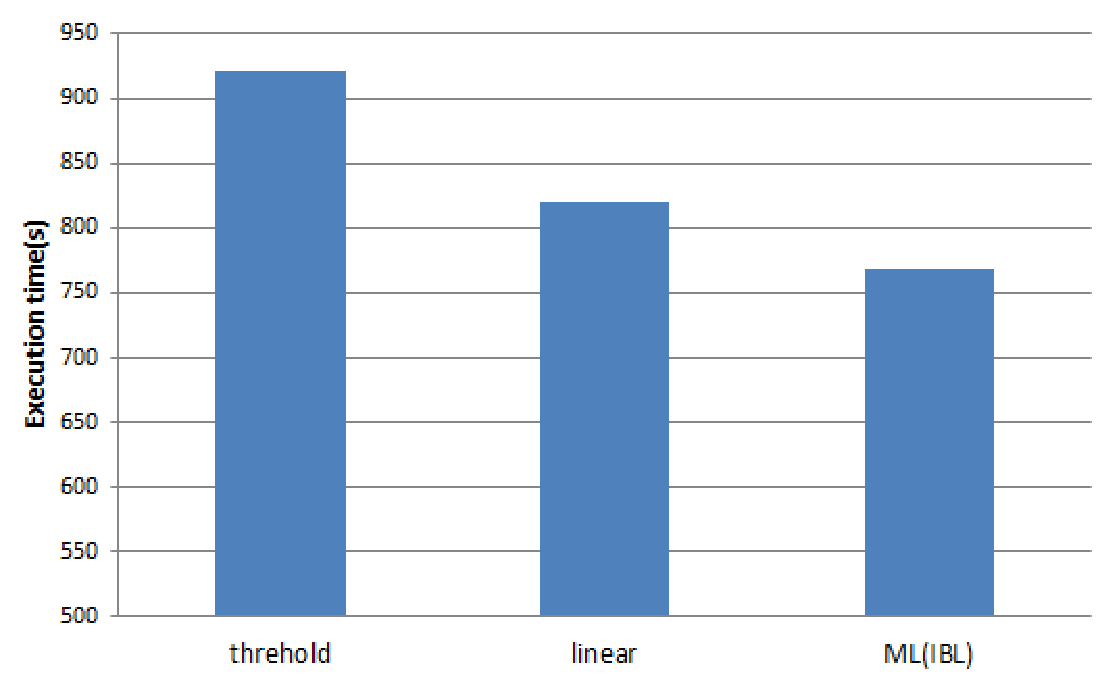
\epsfig{file=figs/execution.eps, width=4.5in}
\caption{Total execution time of 150 Linpack runs}
\label{fig:execution}
\end{figure}
%
Figure~\ref{fig:execution} shows total execution time of 150 Linpack runs with
the threshold-based, linear equation-based, and MALMOS (instance-based
learning).
%
For this experiment, I used the threshold- and linear equation-based
scheduling policies derived from the observation of the offloading
performance with the workstation as the remote resource.
%
With three scheduling policies, the mobile devices offloads Linpack to
the laptop equipped Intel Core2 Duo 2.0Ghz processor running CPU load by
Stress, while changing the network bandwidth as described in the previous 
experiment, and I measured tatal execution time of 150 Linpack runs with 
different input date size. 
%
As shown, the threshold-based scheduler has the longest execution
time due to the lowest scheduling accuracy.
%
The linear equation-based scheduler also shows 6.5\% longer execution
time than MALMOS. 
%

\section{Summary}
\label{online:summary}
%
In this Chapter, I proposed a novel machine learning-based mobile offloading
scheduler with online training, MALMOS.
%
MALMOS is designed in a modular fashion to generally apply to any types of mobile
offloading frameworks.
%
Also, I proposed an adaptive online training mechanism in which the
online training phase and runtime scheduling phase are dynamically switched
according to the scheduling accuracy.
%
To evaluate our work, I applied MALMOS to DPartner, a Java-based on-demand
offloading framework.
%
Also, I utilized three different machine learning algorithms for the
scheduling classifier and compared the overhead in terms of the training
and classification time.
%
Furthermore, I validated the ability of MALMOS to adapt to various network
conditions and computing power capabilities of the remote computing resources
by comparing the scheduling performance with threshold- and linear
equation-based scheduling policies.
%
In the evaluation, I observed that MALMOS has 10.9\%$\sim$40.5\% higher
scheduling performance than two static scheduling policies under various
network conditions, computing power capabilities of the remote servers, and
application complexity.\\
%












\chapter{COLLABORATION WITH PROXIMITY-AWARE CLUSTERING SYSTEM}
\label{chap:solare}
In this Chapter, I introduce SOLARE, a utility functions based
self-organizing network proximity-aware clustering system which can
lead to a possible performance improvement in conjunction with mobile
offloading frameworks.
%
As mentioned in Chapter~\ref{chap:scheduler} and~\ref{chap:online},
network performance such as latency and bandwidth has a significant
impact on the offloading performance, I believe that SOLARE is able to
achieve an additional performance improvement because of its ability to
organize clusters among peers which have similar network performance. 
%
However, as I will describe in this Chapter, SOLARE is the self-organizing and
managing clustering system utilizing a peer-to-peer overlay network as
an underlying substrate to place SOLARE nodes in a synthetic network
coordinate space and to propagate query messages for searching, joining,
and creating appropriate clusters.
%
Therefore, in order for mobile devices to participate directly in the SOLARE
clustering process as an overlay peer, they are required to implement basic 
functionalities of the peer-to-peer overlay networks such as
bootstrapping overlay, maintaining communication channels (i.e. near and
shortcut connections), and propagating messages from other peers, which incur an
additional overhead in terms of energy consumption and processing cost
for mobile platforms.
%
Nevertheless, there still exist ways for mobile devices to collaborate with
the network proximity-aware clustering system to improve the offloading
performance without performing the functionalities of the peer-to-peer
overlay networks. 
%
One possible collaboration of remote computation offloading with SOLARE
is a seamless service migration to another peer in a same cluster.
%
For example, in the case where a remote resource, which currently
provides computing capabilities for mobile computation offloading,
becomes not available due to resource crashes or network problem, the
offloading service should be migrated to another remote resource.
%
If the mobile device keeps a list of remote resources which guarantee
similar network performance in terms of latency or bandwidth (i.e.
remote resources having the same cluster membership) and seamlessly
hopping into another remote resource in the same cluster, the offloading
service is able to continue without any service disconnection or restart.
%
Thus, with the assist from SOLARE, mobile offloading frameworks do not
have to repeat the service discovery process to find another remote
resource which has the best network performance and the offloading
service can resume seamlessly.
%
\section{Motivation of SOLARE}
\label{solare:motivation}
In recent years, the structures of large-scale network have been
extended from client-server architectures for traditional web services
to the distributed systems such as Peer-to-Peer (P2P) networks and
Distributed Hash Tables (DHTs)~\cite{chord, can, tapestry}.
%
Particularly, distributed systems have been increasingly applied to
applications including online gaming, content distribution networks, and
storage systems.
%
One of the key challenges posed by these systems is locating or
connecting a subset of nodes that satisfy user-demands with respect to
network proximity.
%
In distributed online gaming services, for example, players seek to
organize cluster so that those in the same cluster can experience low
latency to each other and enjoy the game without delay perceived by
users.
%
In addition, the supply of powerful commodity computers and the
availability of high speed Internet have enabled grid computing
environments capabilities.
%
In such environments, latency-sensitive applications such as parallel
processing tasks and workflows benefit from proximity among workers, and
the ability to discover resources which satisfy job demands and are
bound by pair-wise latency constraints is important.
%
For such reasons, the inherent support for large-scale systems to
self-organize into clusters that guarantee a certain degree of network
proximity allows middleware and applications to seamlessly discover
resources that are close in a network latency sense.
%
With the approach described in this Chapter, proximity-aware queries can
be efficiently performed through scalable P2P queries within the
self-organized cluster(s) that a node belongs to.\\
%
SOLARE is a peer-to-peer, utility function based self-managing system
that self-organizes clusters in a proximity-aware structured overlay
topology.
%
To do this, I rely on a structured P2P network as underlying global
overlay network and a self-organizing, decentralized network coordinate
system.
%
As reviewed in the next section, there have been a number of related
approaches whereby nodes are clustered based on certain criteria, but to
the best of our knowledge, this work proposes the first implementation
which applies utility functions and network coordinates for the
clustering process.
%
The main idea of SOLARE is that each node searches and joins the highest
utility valued cluster.
%
On the other hand, if there is no cluster whose utility is greater than
the user-defined threshold, the node creates a new cluster declaring its
own coordinate as the virtual center of cluster.
%
Furthermore, a node periodically monitors the status of the cluster that
it is currently involved in so that the node migrates to another cluster
whenever the utility is dropped below a threshold.
%
In this system, migrating clusters means changing the cluster membership
rather than physically moving from one cluster to another cluster.
%
In order to calculate the utility of clusters, I select the distance to
the virtual center of the cluster and the size of the cluster (i.e. the
number of current cluster members) as utility properties.
%
All participants are located in a 2-dimensional space such that each
node has the ability to calculate the Euclidean distance to any points
of 2-dimensional space or other nodes using a Vivaldi network coordinate
system~\cite{vivaldi}.
%
It is important to note that SOLARE is independent of the network
coordinate system.
%
In fact, even though I adopt the Vivaldi network coordinate system,
other related approaches such as GNP~\cite{gnp} and PIC~\cite{pic} can be used for the core of
network latency prediction of SOLARE as well.
%
While this Chapter focuses on latency-based network coordinates,
approaches that consider a bandwidth-based coordinate systems, such as
Sequoia~\cite{ramasu, treeness} can be also considered.
%

\section{Related Work}
\label{solare:related}
\subsection{Clustering approaches on distributed systems}
\label{solare:clustering}
Similar studies to this work have been done in order to offer
proximity-based routing protocols.
%
In~\cite{locality} , the Plethora routing core employs a two-level overlay architecture
with global overlay and local overlays.
%
In particular, local overlays rely on the organization of the Internet
as a collection of Autonomous Systems (ASs) so that they serve as caches
to provide data locality.
%
IP-based clustering for P2P networks has no need for active measurement
of latencies, minimizing system maintenance cost~\cite{ipclustering}.
%
Instead, the authors provide a simple method for the construction of
clusters based on static, readily available information (i.e. IP
address) proving the correlation among common UP prefix length of
communication nodes and latency.
%
The above approaches, however, use only static information without any
measurements, which makes it difficult to handle dynamic network
changes.
%
Cantin et al.~\cite{cantin} adopt the Quality Threshold (QT) algorithm to propose a
self-organized clustering scheme which is built on an existing Internet
coordinate system.
%
Also, they present two variants of distributed clustering algorithm: one
aims at reduction of the clustering construction time, the other tries
to minimize the overhead of the clustering process.
%
Nevertheless, each node needs to perform the computation for QT
algorithm as well as calculating the distance between its first- and
second-order neighbors, introducing additional overheads.
%
The novelty which distinguished this work from the aforementioned
approaches is that this work is a fully decentralized and autonomous
approach, not relying upon any central units such as servers, super
peers, cluster heads or landmarks but utilizing utility functions.\\
%
Clustering techniques have been also adopted in other domains such as
network modeling and performance evaluation.
%
In~\cite{filesharing}, the authors show that both geographical and interest-based
clustering properties inherently exist and can be leveraged to improve
the search mechanisms in file sharing systems using P2P networks.
%
Bu et al.~\cite{bu} provide the Internet topology generator using the cluster
coefficient.
%
Also, wireless sensor networks achieve prolonging the lifespan and
reducing the overhead via cluster-based protocols~\cite{clusterrouting,
energyintra, cao}.
%

\subsection{Utility functions in autonomous systems}
\label{solare:utility}
Utility functions provide a natural and advantageous framework for
achieving self-optimization in autonomic computing~\cite{utilityself}.
%
In fact, applying utility functions to autonomic systems has been done
in various studies.
%
In~\cite{william, unity}, the authors have proposed utility-based resource allocation system
consisting of a number of logically separated application environments
each having an independent utility function.
%
Along with application environments, a global resource arbiter performs
the allocation of resources optimizing the summation of utility
functions from application environments.
%
Similar work has been considered in~\cite{directed}.
%
In this work, however, utility is described with respect to low-level
resources such as CPU, disk, and memory instead of system-level
attributes.
%
In~\cite{cooling}, the authors propose an energy efficient cooling system for data
centers applying utility functions.
%
It formulates simple utility functions that describe a trade-off between
energy and temperature and shows how to optimize a setting of control
parameters, fan speeds and on/off state of air conditioners, using
utility functions.
%
Grandis et al.~\cite{grandis} present the fundamental steps of non-analytic approach on
leveraging utility functions at the application level.
%
Also, they apply their approach to two different case studies, FTP
download and log explosion.
%

\begin{figure}
\centering
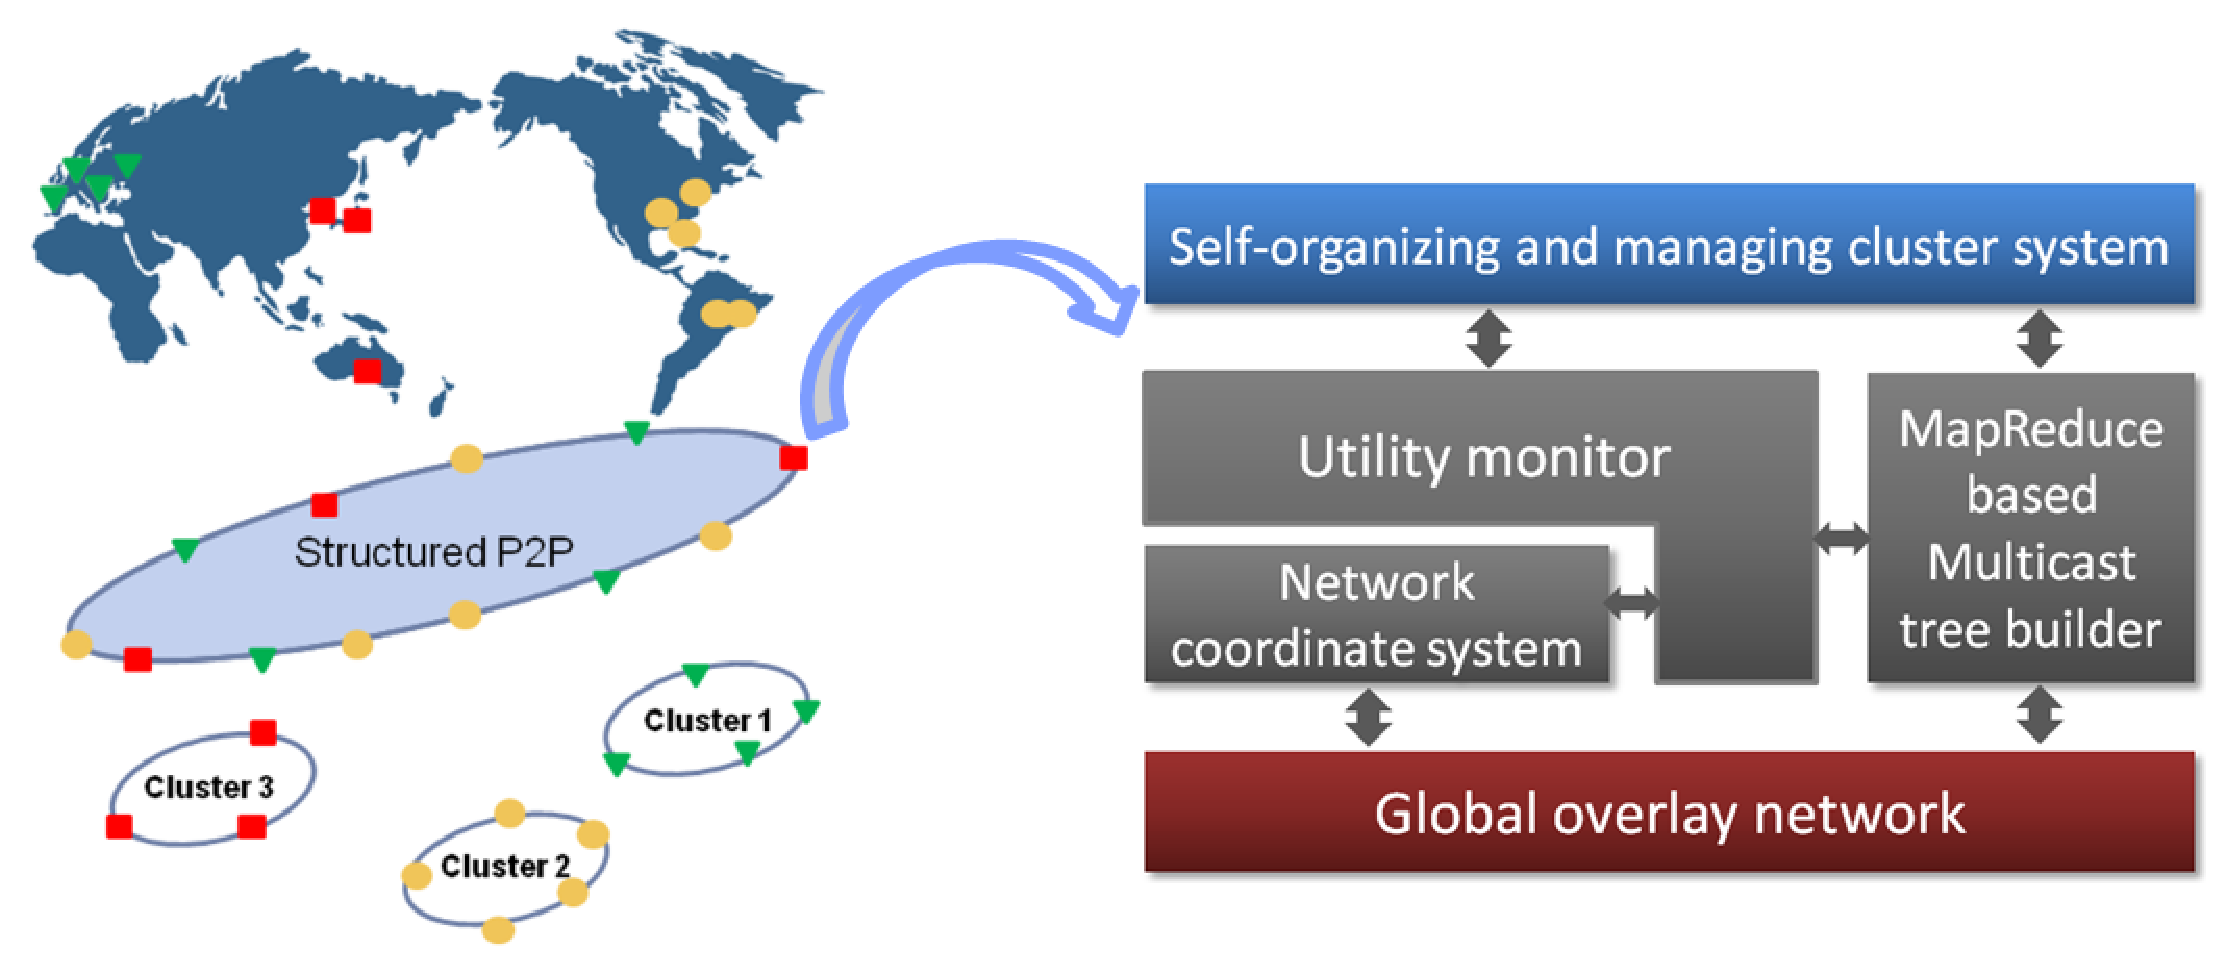
\epsfig{file=figs/solare_structure.eps, width=5.5in}
\caption{Self-organizing latency-aware resource ensemble}
\label{fig:solare}
\end{figure}
%

\section{System Model and Architecture}
\label{solare:architecture}
The main goal in SOLARE is to construct utility functions-based,
self-organizing and self-managing cluster systems such that nodes join
highest ranked cluster with respect to its own preference expressed by a
utility function.
%
The system assumes a global, large-scale structured P2P overlay, from
which virtual clusters are self-organized as sub-overlays based on the
SOLARE algorithm.\\
%
Figure~\ref{fig:solare} illustrates the base concept of the SOLARE
system.
%
In this figure, three small-scale clusters self-organize as virtual
sub-overlays (triangle, circle, square) of the main global overlay based
on their network coordinates and utility functions.
%
Furthermore, each node monitors the cluster that it is currently
involved in, so if its utility value drops below a threshold due to
dynamic changes in network conditions, it migrates to another cluster to
improve cluster utility.
%
Consider, for example, nodes that are geographically distributed and
connected to a large-scale overlay with millions of nodes.
%
Assume a node wishes to connect to 100 nodes or more which are within 50
milliseconds of latency (i.e. round trip time).
%
This node specifies its desirable cluster characteristics in terms of a
utility function, and takes part in SOLARE on top of global overlay
network, requesting information from existing clusters through a
bounded-multicast query mechanism which discovers which nodes belong to
clusters that would maximize the node's utility.
%
Finally, the node makes a decision on the best-suitable cluster based on
its requirements.
%
These steps involve the modules shown in Figure~\ref{fig:solare}
(right).
%
In this section, I describe the main constituents of SOLARE.
%

\subsection{Structured P2P network as global overlay}
\label{solare:global}
The global overlay network provides an underlying substrate to place
nodes in a network coordinate space and to propagate query messages.
%
As soon as nodes join the global overlay network, they calculate their
positions and send a query message for cluster information.
%
I choose Symphony~\cite{symphony}, a 1-dimensional Kleinberg small-world network as
underlying global overlay network, and build upon the implementation of
Brunet~\cite{brunet}, a general P2P software framework.
%
Symphony organizes nodes in a ring topology in which each node has a
constant number of near connections and \textit{log(N)} number of
shortcut connections, where \textit{N} is the number of nodes in the
network.

\subsection{Query propagation system}
\label{solare:query}
One of the essential features of a self-organizing cluster system is how
nodes locate a candidate set of clusters in an efficient way, without
missing high-quality clusters to join in terms of the user demand.
%
With the purpose of improving the cluster searching quality with
scalable query mechanism, I employ Map and Reduce functions on a
self-organizing multicast tree~\cite{lee}.
%
This approach is based on a multicast tree builder consisting of two
parts: Map and Reduce functions which process the propagation of query
and merge the results, and a multicast tree builder that is the
recursive algorithm to build a multicast tree.
%
MapReduce is a software framework associated with information processing
on large data sets~\cite{mapreduce}.
%
The Map function works on a set of data to generate intermediate value
while the Reduce function merges all intermediate value associated with
the identical intermediate key.
%
In conjunction with Map and Reduce functions, the multicast tree
builder assists in propagating a message in a scalable manner (with
\textit{log(N)} depth) by building a multicast tree using structured
shortcut and near connections~\cite{deetoo}.
%
This approach can be applied recursively to
sub-overlays~\cite{bootstrap} such that the
same mechanism used across the overlay to discover candidate clusters to
be joined, can also be used at the application layer to discover nodes
that satisfy requirements within a proximity-aware cluster.\\
%
\begin{figure}
\centering
\subfigure[Symphony topology] {
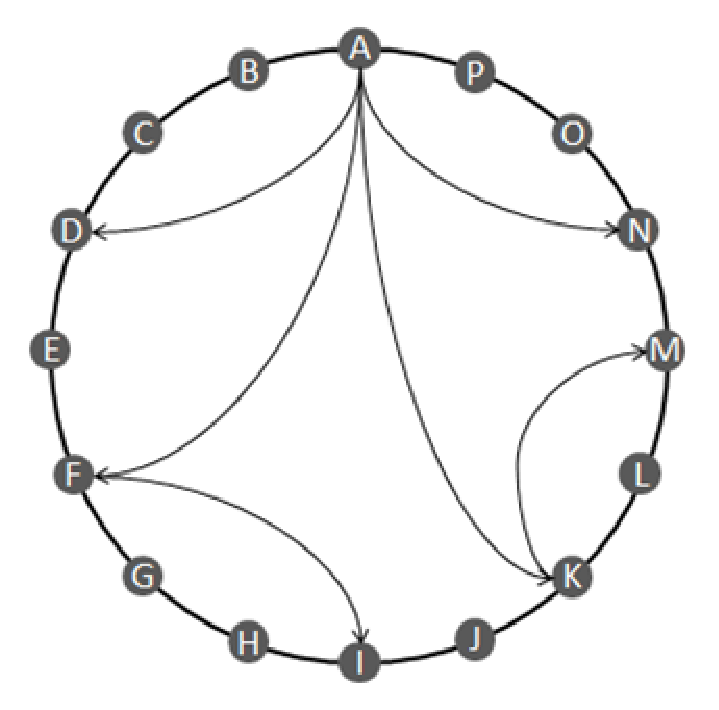
\includegraphics[width=2.3in]{figs/symphony.eps}
\label{fig:symphony}
}
\subfigure[Multicast tree] {
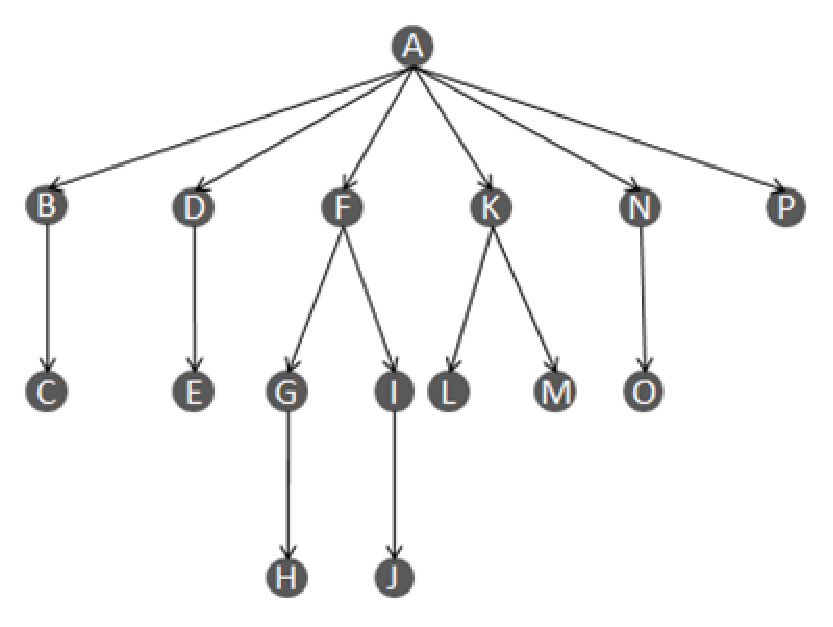
\includegraphics[width=2.3in]{figs/multicast_tree.eps}
\label{fig:multi}
}
\caption{Map and Reduce functions based multicast tree builder}
\label{fig:treebuild}
\end{figure}
%
Figure~\ref{fig:treebuild} shows how Map and Reduce functions based
multicast tree builder creates the multicast tree and propagates a query
on top of symphony.
%
Assuming that node A is an origin node which sends a message over the
entire network (or alternatively a bounded region of the network, in
this example the bounds are A and P).
%
Node A sends a message to nodes B, D, F ,K, N and P (which are referred
as node A's child nodes) through its near connections and short
connections by setting sub-multicast range as [B,D), [D,F), [F,K),
[K,N), [N,P) and [P,A-1), respectively.
%
Nodes which receive the message send the message to their neighbors
within sub-multicast range.
%
Differently stated, node B has the responsibility of building the
multicast tree in range [B,D).
%
In a such way, nodes multicast the message until there is no connection
and the multicast tree is built as shown in Figure~\ref{fig:multi}.
%
Each node in the tree computes a Map function, and results are
back-propagated through the tree, with each node computing a Reduce
function on the values they receive from its children.
%
The strength of Map and Reduce functions based multicast tree builder
lies in the ability to parallelize the Map and Reduce functions,
providing the ability to select a subset of results based on utility
functions, thereby bounding the bandwidth used in such queries.
%
With a Reduce function that bounds the number of results returned by a
node by a constant, the average per-node bandwidth consumed by a query
is constant~\cite{deetoo, lee}.
%

\subsection{Network coordinate system}
\label{solare:coordinate}
A network coordinate system places nodes in some synthetic network
coordinate space such that each node can predict the latency to other
nodes.
%
One example is Vivaldi, which achieves this by modeling a spring
system~\cite{vivaldi}.
%
Due to the triangle inequality of the network coordinate space, the Vivaldi
network coordinate system attempts to minimize the error between the
predicted distance and actual latency instead of exploiting accurate
coordinates.
%
Each node involved in the Vivaldi network coordinate system measures the RTT
(Round Trip Time) to its neighbor \textit{n$_{i}$} whose coordinate is
\textit{x$_{i}$} and computes the error \textit{e} between measured RTT
and Euclidean distance of its coordinate and \textit{x$_{i}$}.
%
Finally, it updates its new coordinate as follows:
%
\begin{equation}
	\textit{Coordinate$_{new}$} = \textit{Coordinate$_{previous}$} +
\textit{$\delta$} \times \textit{e} \times \textit{D} 
\label{equ:coordinate}
\end{equation}
%
where $\delta$ is the timestep which quantifies the size of step toward
new coordinate and \textit{D} is the direction to new coordinate.
%
An adaptive value of $\delta$ provides the control on the fraction of
the step so that each node converges towards approximately accurate
position quickly and precisely.
%
The Vivaldi system has been implemented on top of Brunet and is used as
a basis for the experiments in this work.
%
As soon as each node joins the global overlay, it runs the Vivaldi
network coordinate system to obtain 2-dimensional coordinates so as to
predict the latency to the candidate clusters as well as the neighbors.
%

\section{SOLARE Modules and Algorithms}
\label{solare:modules}
\subsection{Utility functions}
\label{solare:utility}
A self-organizing and self-managing system needs to serve diverse
requests from a number of users who have different expectations on
service quality.
%
The challenge of this task is not only to approximately satisfy the
demands from all the users but also to maximize the utilization of
entire system.
%
In this work, I make use of utility functions as a practical scheme of
achieving self-organizing and self-managing cluster system in which each
node describes its own preference on joining a cluster, and makes the
best decision given a set of clusters.
%
To apply utility functions to this system, first of all, I identify two
attributes that nodes attempt to optimize.\\
%
\textbf{Distance to the cluster (\textit{D$_{i}$}).} means the Euclidean
distance between the coordinate of node and a virtual center of a
particular cluster, \textit{i}.\\
%
\textbf{Size of cluster (\textit{S$_{i}$}).} is the size of a cluster,
that is  the number of cluster members which involve in a particular
cluster, \textit{i}.\\
%
Next, I establish two utility functions, \textit{U$_{distance}$} and
\textit{U$_{size}$}, each expressing the preference on above two
attributes.
%
\begin{figure}
\centering
\subfigure[Utility for Distance(\textit{D$_{max}$} = 100)] {
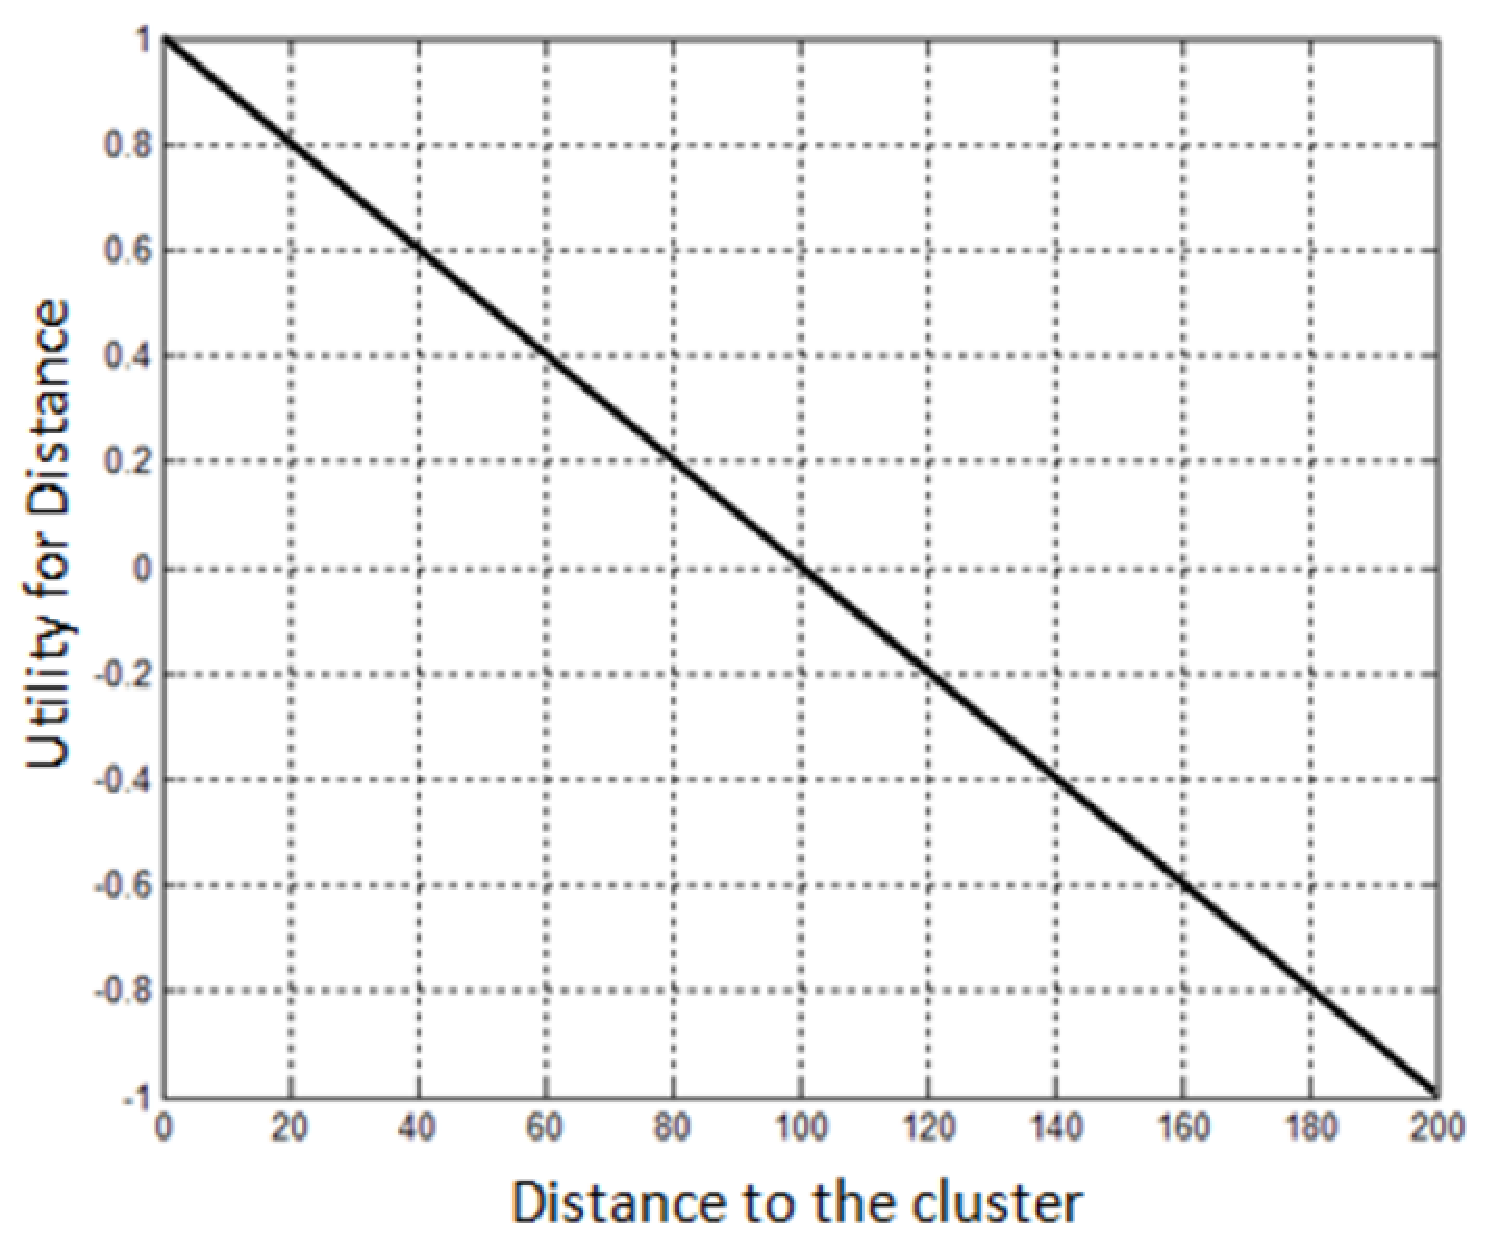
\includegraphics[width=2.7in]{figs/utility_distance.eps}
\label{fig:udistance}
}
\subfigure[Utility for Size(\textit{S$_{min}$} = 100)] {
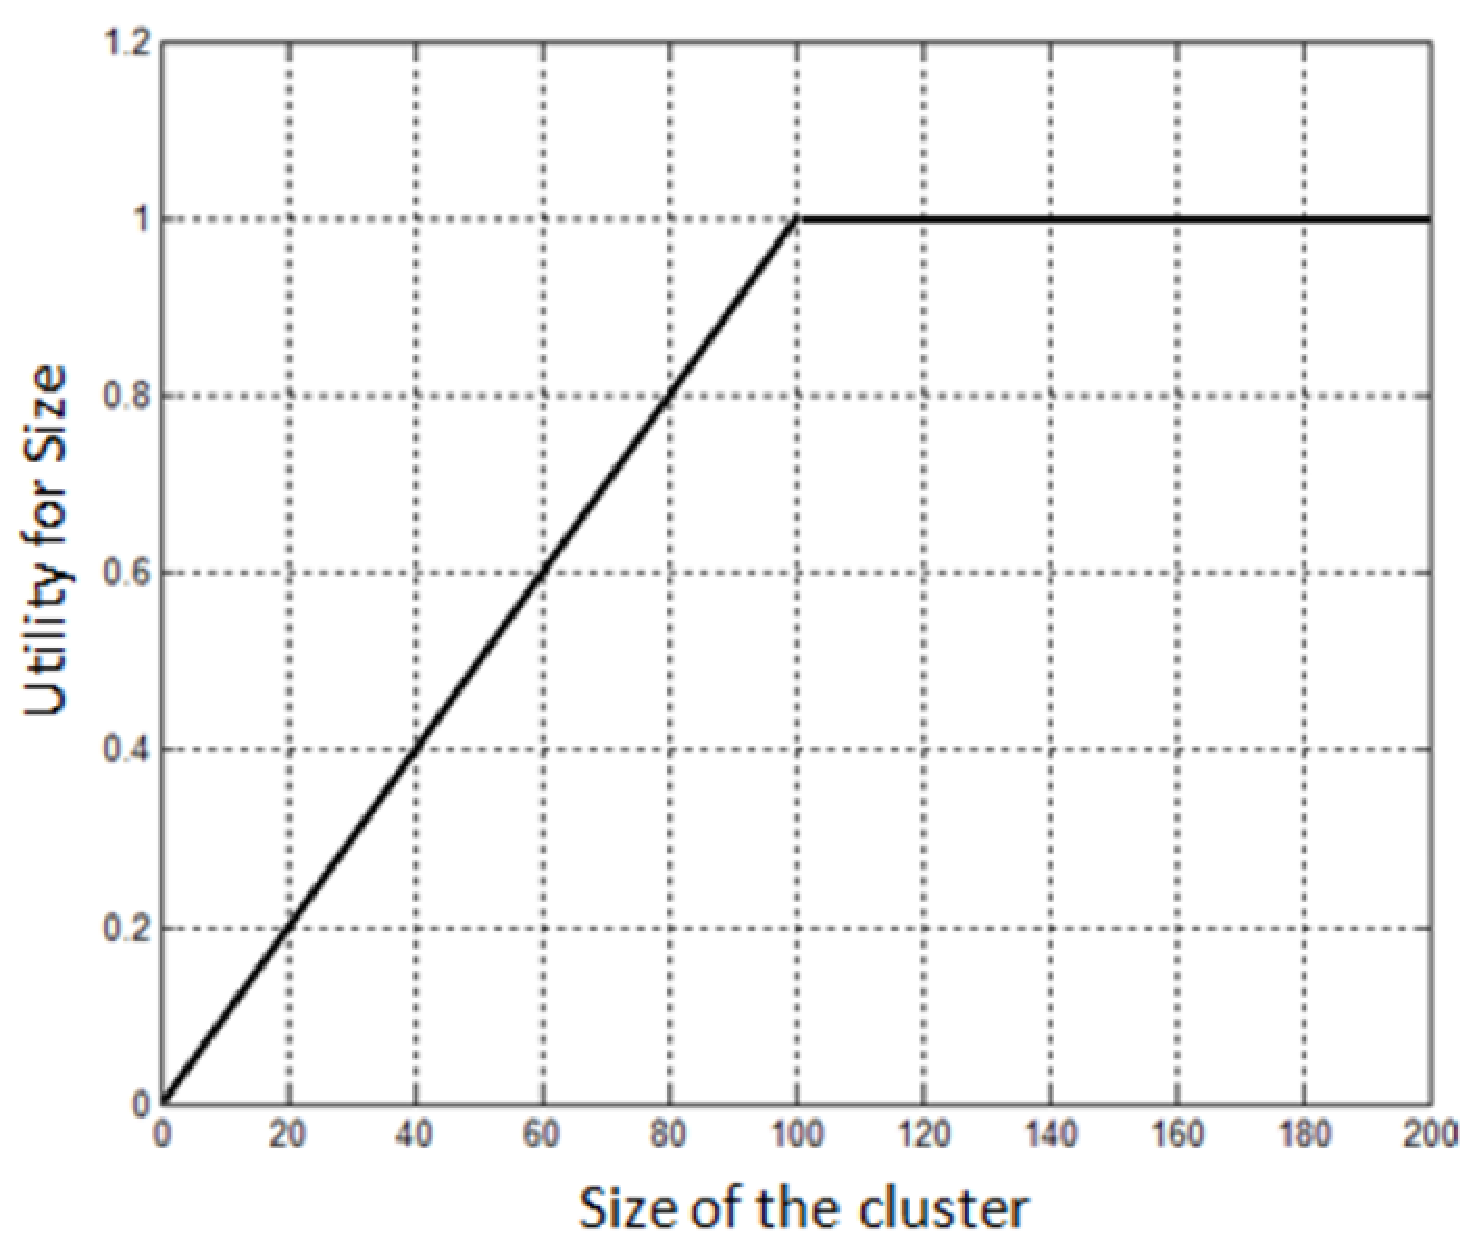
\includegraphics[width=2.7in]{figs/utility_size.eps}
\label{fig:usize}
}
\caption{Example for utility functions for cluster distance and size}
\label{fig:utility}
\end{figure}
%
Figure~\ref{fig:utility} illustrates utility functions \textit{U$_{distance}$} and
\textit{U$_{size}$} that I set in this system.
%
Note that I have two key parameters to configure: maximum tolerance for
distance to the virtual cluster center (\textit{D$_{max}$}) and minimum
preference for cluster size (\textit{S$_{min}$}).
%
The former is the maximum distance to the cluster which has positive
utility value, while the latter means the minimum size of the cluster
which has maximum utility, 1, regardless of the size of the cluster.
%
Users can define their own utility functions by differently setting
these two parameters.
%
Finally, after adding the coefficients for each utility function, I
merge two utility functions into total utility function as
Equation~\eqref{equ:utility} in which each node computes total utility
value for a cluster.
%
\begin{equation}
	\textit{U$_{total}$} = \textit{$\alpha$$_{size}$} \times
\textit{U$_{size}$} + \textit{$\alpha$$_{distance}$} \times
\textit{U$_{distance}$} 
\label{equ:utility}
\end{equation}
%
where \textit{$\alpha$$_{size}$} and \textit{$\alpha$$_{distance}$} are
coefficients for \textit{U$_{size}$} and \textit{U$_{distance}$},
respectively, such that the sum of two values is 1.
%
Similar to \textit{D$_{max}$} and \textit{S$_{min}$}, coefficients for
size and distance are user-definable parameters so that each user
presents the priority among the attributes.
%
\begin{figure}
\centering
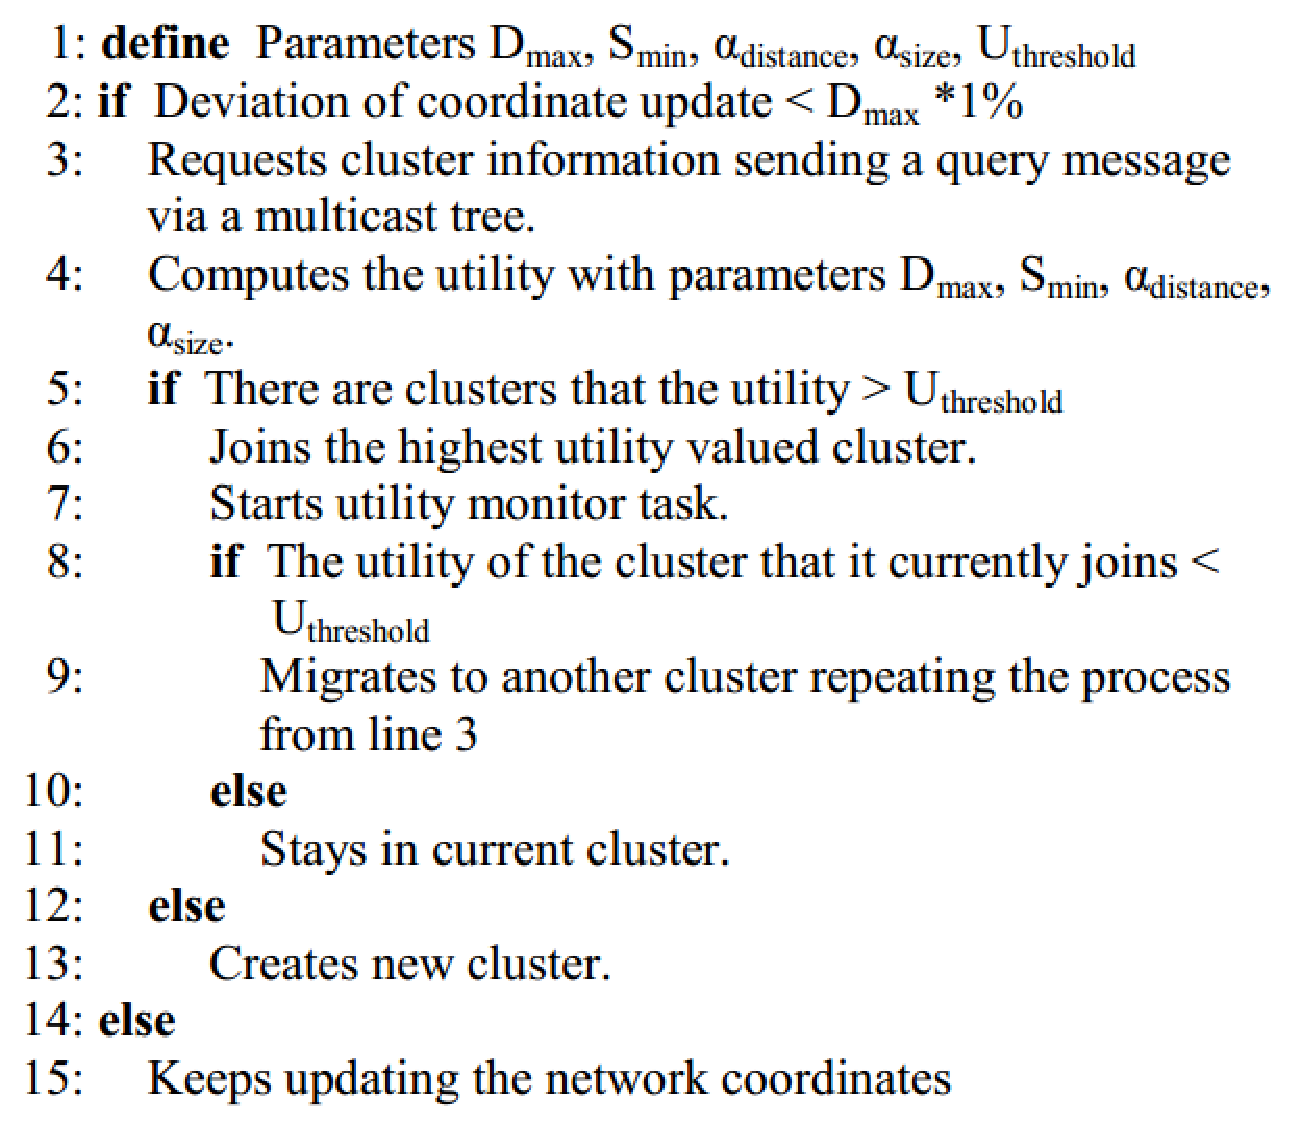
\epsfig{file=figs/solare_algorithm.eps, width=4.3in}
\caption{Pseudo-code for self-organizing and managing clustering system}
\label{fig:solare_algorithm}
\end{figure}
%

\subsection{Self-organizing and managing cluster process}
\label{solare:clusterprocess}
As described in previous section, utility functions represent user
preference on selecting a cluster to join.
%
In this section, I describe how nodes can self-organize the cluster
architecture using utility functions.
%
The main idea of this clustering algorithm is that each node searches
and joins the highest utility valued cluster.
%
On the other hand, if there is no cluster whose utility is greater than
the user defined threshold, nodes create new cluster declaring its own
coordinate as the virtual center of cluster.
%
Furthermore, a node periodically monitors the status of cluster that it
is currently involved in order to migrate to another cluster whenever
the utility is dropped below the threshold.
%
The clustering process is presented in Figure~\ref{fig:solare_algorithm} 
and described in detail as follows.\\
%
Upon joining the global network, a node computes its coordinates in
2-dimensional Euclidean space using Vivaldi network coordinate system.
%
In order to avoid too frequent cluster migrations on the way toward the
accurate position, the cluster process starts after the deviation of
coordinate update becomes relatively small.
%
As soon as node initiates the clustering process, it sends a request
message including its coordinates to find the highest utility valued one
of existing clusters through the multicast tree constructed by Map and
Reduce functions based multicast tree builder.
%
As the response for the request message, all the nodes calculate the
utility of its cluster using the coordinate of the query origin node
with the Map function and compare the utility of its cluster to the
utilities from its child nodes using the Reduce function.
%
Then, nodes send only the information of the highest utility valued
cluster to their parent node of the multicast tree.
%
As a result, the query origin node receives only one response from a
child node, and it can find the highest utility valued cluster with a
lightweight comparison.
%
It is worth noting that Map and Reduce functions at the response phase
help in reducing the number and the size of response messages.
%
After joining the highest utility valued cluster, the node informs
cluster members of its intent to join by multicasting a join message.
%
By counting this type of message, cluster members keep the size of
cluster up to date; they can also periodically query the cluster for
membership count using a Map and Reduce functions multicast query within
the cluster sub-overlay.
%
If utility values of all the existing clusters do not satisfy the demand
of the node (which means that utility values are less than the
user-defined threshold), the node creates a new cluster.\\
%
Creating a new cluster is straightforward.
%
A node generates a random clusterID ranging from 0 to 2$^{160}$-1 which is
identical to the node address space of Symphony.
%
Also, the node declares its current coordinates as the virtual center of
cluster.
%
With doing this, the node can subsequently reply to cluster requests
from other nodes.
%
After first joining the cluster, the node starts a utility monitoring
task.
%
Network status has the possibility to be changed due to the churn and
dynamic changes in traffic in the physical network.
%
Such changes in the network result in the fluctuation of the utility
value and nodes can take the potential advantage from the ability to
migrate from the current cluster to another cluster.
%
The self-managing cluster system needs to deal with this problem.
%
The utility arbiter checks whether utility value is dropped below the
threshold or not.
%
To do this, nodes  periodically calculate the distance to the virtual
center of cluster and count the number of cluster members.
%
If the utility value is dropped below the threshold, nodes repeat above
cluster searching, joining or creating process.\\
%
The main contribution of this work is that the clustering algorithm has
a fully decentralized feature which does not rely upon any central units
such as servers, super peers, cluster heads or landmarks; hence it is
robust against the single point of failure.
%
Because each node holds the information of its own cluster locally, it
is unlikely that node failures or leave affects the performance of the
whole system.
%
Also, the destruction of cluster which does not have any cluster members
at all is done without additional process.
%
The departure of last cluster member means that the cluster does not
exist in the network.
%

\section{Performance Evaluation}
\label{solare:evaluation}
In this section, I present results from simulation based analysis for
SOLARE.
%
In this evaluation, I use Brunet in event-driven simulation
mode~\cite{david} and
configure simulated latencies using King dataset~\cite{king} with 1740 nodes.
%
Brunet simulator uses simulated virtual time based upon an event-driven
scheduler instead of real time.
%
While existing simulators such as p2psim~\cite{p2psim}, NS2~\cite{ns2},
and netmodeler~\cite{netmodeler} are
algorithm-oriented simulators which aim to evaluate algorithm
validation, Brunet simulator has the ability to simulate the deployed
system stack as well as algorithm using a specialized transport layer to
avoid the overhead of using TCP or UDP on the host system.
%
The specialized transport uses datagrams to pass messages between nodes,
thus from an individual node's perspective, it is very similar to a UDP
transport and can simulate both latency and packet dropping.
%
\begin{figure}
\centering
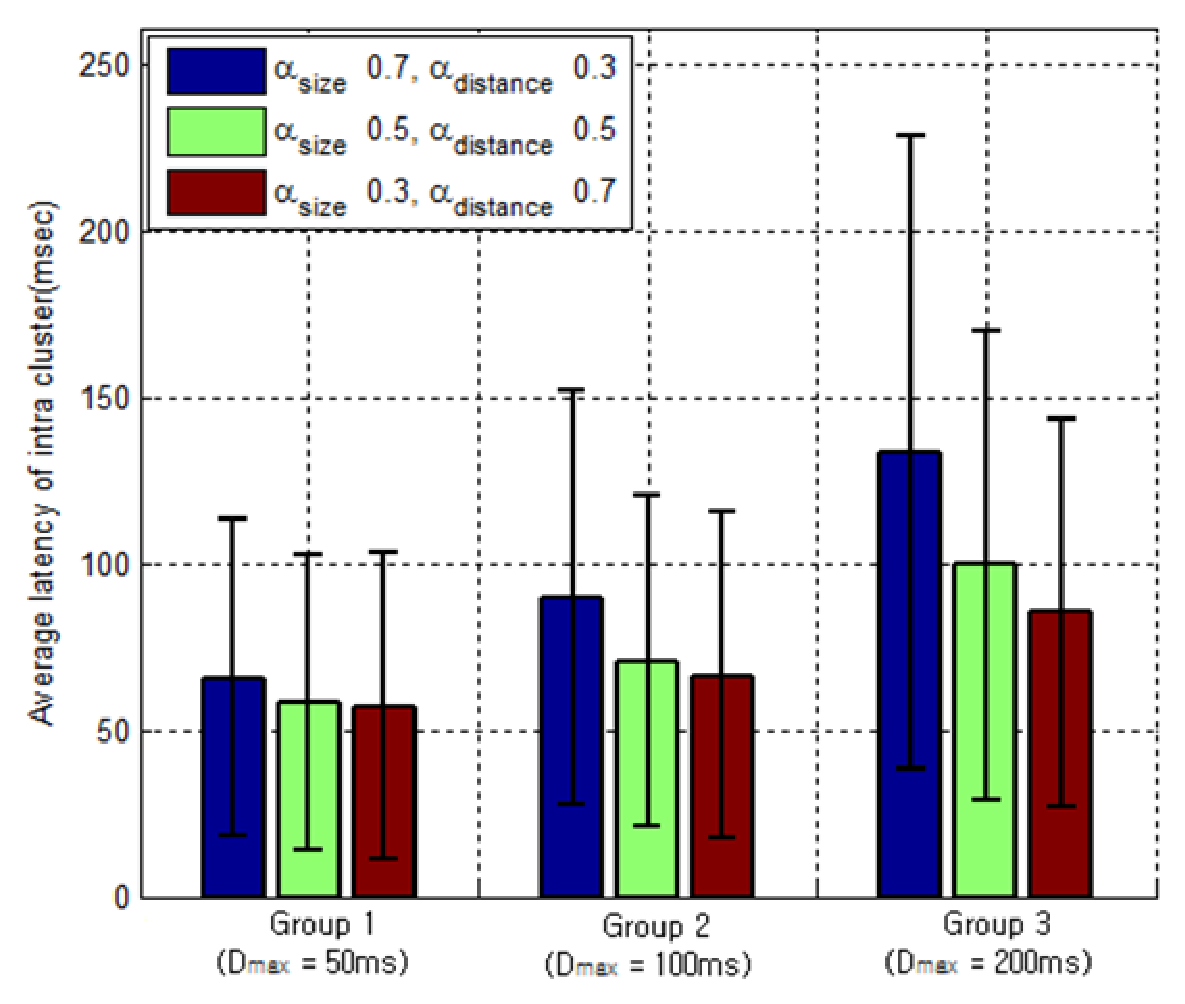
\epsfig{file=figs/latency_s50.eps, width=4.0in}
\caption{Average latency of intra-cluster with \textit{S$_{min}$} = 50}
\label{fig:latency50}
\end{figure}
%
\begin{figure}
\centering
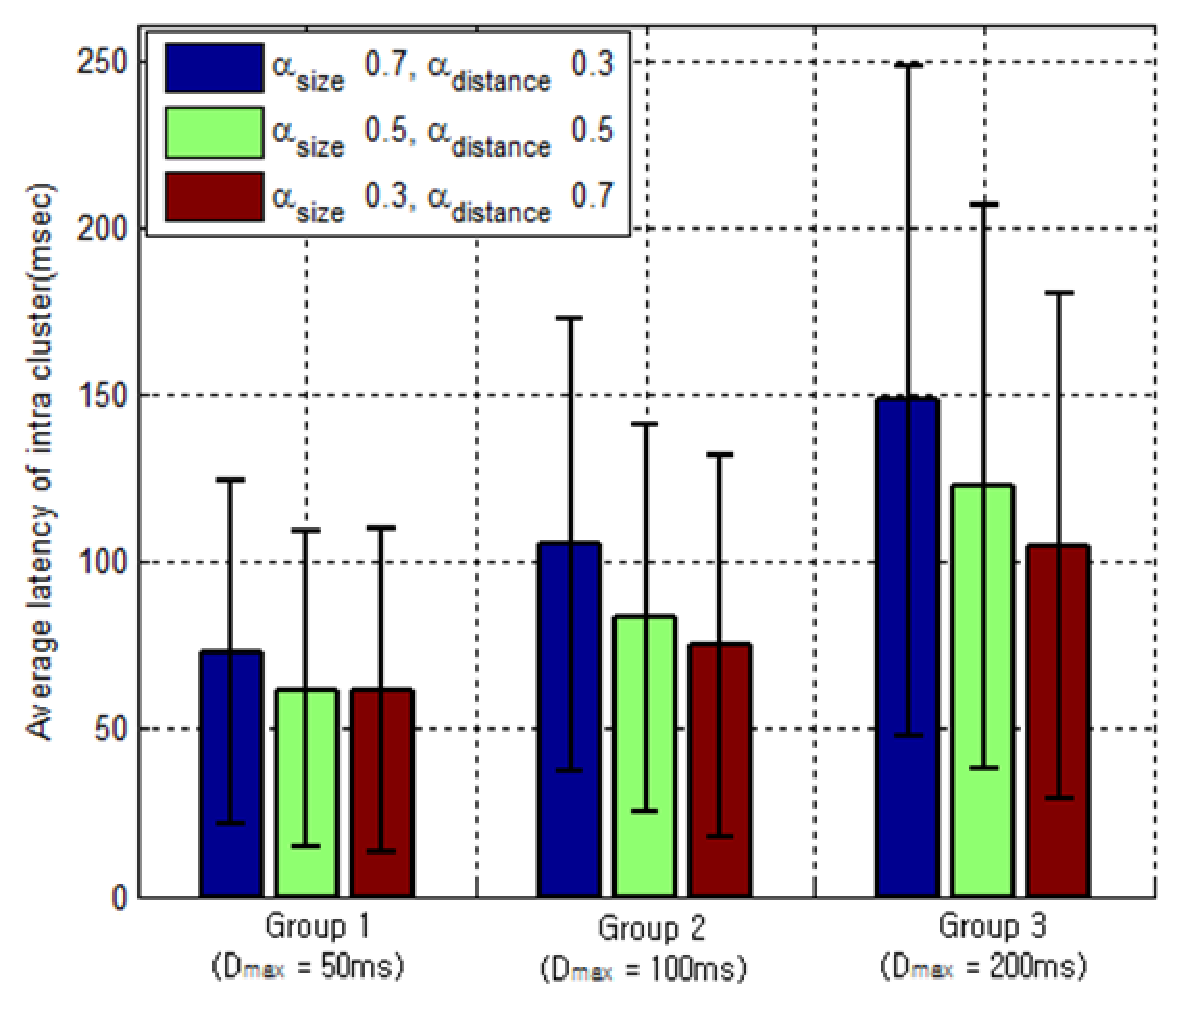
\epsfig{file=figs/latency_s100.eps, width=4.0in}
\caption{Average latency of intra-cluster with \textit{S$_{min}$} = 100}
\label{fig:latency100}
\end{figure}
%
\begin{figure}
\centering
\epsfig{file=figs/latency_s200.eps, width=4.0in}
\caption{Average latency of intra-cluster with \textit{S$_{min}$} = 200}
\label{fig:latency200}
\end{figure}
%

\subsection{Inter-cluster latencies}
\label{solare:interlatency}
Since \textit{D$_{max}$} is the maximum distance to the virtual cluster
center that a node expects when it searches a cluster to join, I can
refer \textit{D$_{max}$} as the radius of cluster.
%
Therefore, upon joining a particular cluster, nodes are able to expect
at most 2$\times$\textit{D$_{max}$} of the latency between cluster
members.
%
To evaluate the performance of this clustering algorithm, I measure
intra-cluster latencies -- the latency between cluster members in the
same cluster.
%
I set \textit{D$_{max}$} to 50ms, 100ms, and 200ms, and
\textit{S$_{min}$} to 50, 100, and 200, respectively.
%
Also, \textit{$\alpha$$_{distance}$} is varied with 0.3, 0.5, and 0.7 (i.e.
\textit{$\alpha$$_{size}$} is 0.7, 0.5, and 0.3).
%
Figure~\ref{fig:latency50},~\ref{fig:latency100},
and~\ref{fig:latency200} show the average and standard deviation of
intra-cluster latency with various parameters setup.
%
First of all, I observe that all the combinations of the parameters
satisfy 2$\times$\textit{D$_{max}$} in terms of the average latency of
intra-cluster.
%
Specially, even in all cases that \textit{D$_{max}$} is 50ms, the
average latency is less than 2$\times$\textit{D$_{max}$}, 100ms.
%
From this result, I note that even though nodes only measure the
distance to the virtual center of cluster, it does not prevent nodes
from getting neighbors who are mostly within \textit{D$_{max}$}.\\
%
Second, by comparing three bars which have different colors in each
group, I observe that the larger coefficient for distance,
$\alpha$$_{distance}$ is, the smaller average intra-cluster latency is.
%
In the case that \textit{D$_{max}$} is 50ms in
Figure~\ref{fig:latency50}, the average
intra-cluster latency with $\alpha$$_{distance}$ of 0.7 is reduced by
11\% and 2\% compared with $\alpha$$_{distance}$ of 0.3 and 0.5,
respectively.
%
Such this difference becomes much clearer as \textit{D$_{max}$}
increases showing 35.9\% and 14.4\% of decrease compared the case of
$\alpha$$_{distance}$ of 0.7 with the cases of 0.3 and 0.5 and
\textit{D$_{max}$} of 200ms.
%
The standard deviation when $\alpha$$_{distance}$ is set to 0.7 is also
decreased by 38.7\% and 17.2\% compared to $\alpha$$_{distance}$ of 0.3
and 0.5 in the Group1 of Figure~\ref{fig:latency50}.
%
Furthermore, I observe that the minimum preference for cluster size,
\textit{S$_{min}$} does not affect the average intra-cluster latency by
observing the same pattern of average latency regardless of
\textit{S$_{min}$} in Figure~\ref{fig:latency100}
and~\ref{fig:latency200}, even though there is a slight trend upward of
average latency as \textit{S$_{min}$} increases.
%
\begin{figure}
\centering
\epsfig{file=figs/cluster_population.eps, width=5.0in}
\caption{The number of created clusters and the population of clusters}
\label{fig:population}
\end{figure}
%
\begin{table}
\centering
\caption{Simulation setup with various parameters setup}
	\begin{tabular}{c|c|c|c|c}
	\hline
	\ & \textit{D$_{max}$} & \textit{S$_{min}$} & $\alpha$$_{distance}$ &
$\alpha$$_{size}$ \\
	\hline
	Simulation A & 200ms & 200 & 0.3 & 0.7 \\
	Simulation B & 100ms & 100 & 0.5 & 0.5 \\
	Simulation C & 50ms & 50 & 0.7 & 0.3 \\
	\hline
	\end{tabular}
\label{table:simulation_setup}
\end{table}
%
\begin{figure}
\centering
\epsfig{file=figs/percentage_s50.eps, width=4.0in}
\caption{Percentage of nodes having more cluster member than \textit{S$_{min}$} = 50}
\label{fig:population50}
\end{figure}
%
\begin{figure}
\centering
\epsfig{file=figs/percentage_s100.eps, width=4.0in}
\caption{Percentage of nodes having more cluster member than
\textit{S$_{min}$} = 100}
\label{fig:population100}
\end{figure}
%
\begin{figure}
\centering
\epsfig{file=figs/percentage_s200.eps, width=4.0in}
\caption{Percentage of nodes having more cluster member than
\textit{S$_{min}$} = 200}
\label{fig:population200}
\end{figure}

\subsection{The number of cluster members}
\label{solare:clustermember}
In addition to intra-cluster latencies, I measure the cluster size which
takes the other part of total utility function.
%
To measure the cluster size, I took snapshots of the number of created
clusters and cluster members for each node when all nodes join a
cluster.
%
Due to the limitation of space, the results from only three simulations
of all the simulations I performed are represented in
Figure~\ref{fig:population} depicting the number of created clusters and
the population of clusters.
%
Table~\ref{table:simulation_setup} summarizes the parameters setup for
the simulation.
%
Firstly, in simulation A, I observe that only 16 clusters are created
and 98.5\% of nodes are included in only one cluster.
%
In fact, for this simulation set, \textit{D$_{max}$} and
$\alpha$$_{size}$ are set to 200ms and 0.7 which are most likely to
organize the largest cluster of all the simulations.
%
However, as \textit{D$_{max}$} and $\alpha$$_{size}$ decrease, the number
of created clusters increases and the population is also distributed
throughout the created clusters.
%
Particularly, for the case of simulation C in which nodes require
relatively small cluster size but much closer cluster members, 155
clusters are created and nodes join clusters more evenly than simulation
A or B.
%
Furthermore, each result from three simulations show one big cluster
including at least 58\% of nodes which is caused by the type of utility
function for cluster size I used.
%
From Chapter~\ref{solare:utility}, recall the baseline of utility
function for cluster size in such that nodes prefer larger cluster size
without an upper limit.
%
If I consider another type of utility function which defines upper limit
of cluster size, one major cluster may disappear and the population of
cluster should become more even.\\
%
To summarize the evaluation of quantitative performance, as shown in
Figure~\ref{fig:population50},~\ref{fig:population100},
and~\ref{fig:population200}, I consider the percentage of nodes which have more cluster
members than \textit{S$_{min}$}.
%
Figure~\ref{fig:population50} shows that as \textit{D$_{max}$} and
$\alpha$$_{size}$} become larger, more nodes can obtain same or
more cluster members than \textit{S$_{min}$} 
%
Although, indeed, only 54\% of nodes have more cluster members than
\textit{S$_{min}$} with 50ms of \textit{D$_{max}$} and 0.3 of
$\alpha$$_{size}$, in the case with 200ms of \textit{D$_{max}$} and 0.7
of $\alpha$$_{size}$, almost 98\% of nodes satisfy the minimum
preference for cluster size, \textit{S$_{min}$}.
%
Regardless of setting of \textit{S$_{min}$}, the same trend is observed
in Figure~\ref{fig:population100} and~\ref{fig:population200} where
\textit{S$_{min}$} is set to 100ms and 200ms with more than 97\% and
98\% of nodes satisfied with \textit{S$_{min}$}.
%
Thus, I can confirm the correctness of this clustering system with the
result of the number of cluster members.
%

\subsection{Adaptability to dynamic network conditions}
\label{solare:adaptability}
Finally, I discuss the adaptability of SOLARE.
%
Network status can be changed dynamically due to the node joining,
leaving, and the change of network latencies.
%
Therefore, nodes should adapt to dynamic network status for the ability
to self-manage the cluster system.
%
After a node joins the cluster, it periodically updates the utility for
its cluster, so if utility is dropped below the threshold, a node
repeats the cluster joining procedure to migrate into another high
utility-valued cluster.
%
To evaluate the adaptability of this system, I observe the percentage of
the number of nodes which need the cluster migration and average utility
value over the entire network.
%
Instead of directly modifying network latency at the simulation
environment, I assume that new joining in global network can cause the
change of the position of nodes in the network coordinate space.
%
Figure~\ref{fig:rejoin} shows the percentage of the number of nodes
which need to migrate from current cluster into another cluster due to
the negative utility value.
%
Because 1740 nodes sequentially join in global network with 500
milliseconds of interval in the simulation scenarios as described in
Table~\ref{table:simulation_setup}, all nodes complete joining the
global network around 15 minutes after starting the simulation.
%
In the case of simulation A where \textit{D$_{max}$} and
\textit{S$_{min}$} are set to 50ms and 50, respectively, cluster
migrations happen most frequently.
%
In fact, because parameters for simulation C imply the smallest cluster,
it is most likely that cluster migrations occur by slight change of the
coordinate.
%
However, after all nodes join the global network and step into correct
position, the occurrence of migrations decreases and the percentage of
nodes which migrate to another cluster is dropped below 5\% after 30
minutes from starting the simulation.\\
%
\begin{figure}
\centering
\epsfig{file=figs/rejoin.eps, width=4.0in}
\caption{Percentage of the number of rejoining nodes}
\label{fig:rejoin}
\end{figure}
%
\begin{figure}
\centering
\epsfig{file=figs/average_utility.eps, width=4.0in}
\caption{Average utility value}
\label{fig:avgutility}
\end{figure}
%
Such a pattern of the occurrence of migrations is observed in the case
of simulation B with 100ms of \textit{D$_{max}$} and 100 of
\textit{S${min}$}, but the percentage of nodes which migrate into
another cluster is less than simulation C because of the parameters set
which means bigger cluster than the case of simulation C.
%
Especially, in Simulation A where the biggest cluster is set, nodes
barely migrate, because the change of the coordinate of nodes occurs
within a cluster.
%
Also, I can observe from Figure~\ref{fig:avgutility} that after the
percentage of nodes which migrate is saturated or dropped drastically,
the average utility value over the entire network is also saturated
which means that the majority of nodes place at correct position and
stay in current cluster.
%
Note that the difference of the utility value saturated can be inferred
from Figure~\ref{fig:population}.
%
Because most of nodes with simulation A, about 98.5\%, are in the same
cluster, it is easy to gain higher utility value for cluster size than
other cases.
%
On the other hand, in the case of simulation C, nodes are distributed
among many clusters, and only 59\% of nodes have more cluster members
than \textit{S$_{min}$}.
%
Consequently, it results in the lowest utility value for cluster size
and total average utility value.
%
%
%\section{Possible Integration with Mobile Offloading Framework}
%\label{solare:integration}
%

\section{Summary}
\label{solare:summary}
In this Chapter, I introduced SOLARE, a peer-to-peer, utility based
self-organizing clustering system which is able to collaborate with
remote computation offloading to achieve the additional offloading
performance improvement.
%
Since the main goal of SOLARE is to organize a proximity-aware
clustering topology, it is possible to provide 
%
In SOLARE, all participants compute themselves the utility for existing clusters
and join highest utility valued cluster.
%
On the other hand, if there is no cluster whose utility is greater than
the user-defined threshold, nodes create a new cluster declaring their
own coordinate as the virtual center of cluster.
%
To establish utility functions, I select the distance to cluster and the
size of cluster as utility properties.
%
Furthermore, the clustering system provides the adaptability for dynamic
network status while each node monitors the cluster that it is currently
joining.
%
After describing the self-organizing and managing clustering procedure,
I evaluated its performance in terms of latencies of intra cluster and
the number of cluster members.
%
Based on the evaluation, I confirmed that setting of parameters, which
form utility functions, can control the properties of clusters such as
latencies of intra cluster and the population of clusters.
%
Additionally, by measuring the percentage of the number of nodes which
need to migrate into another cluster and average utility value, I
presented the adaptability of the system.
%

\chapter{SUMMARY AND FUTURE WORK}
\label{chap:summary}
%
This proposal presents a novel framework which enables remote workload
offloading to trusted remote resources through the
paradigm of extended hardware-layer heterogeneous computing environment.
%
Thus, the proposed framework broadens the range of heterogeneous
computing to remote resources in the network, where offloading services
are dynamically discovered. 
%
The proposed approach accomplishes this by 1) extending the OpenCL framework to
support remote offloading using the TCP/IP networking stack and 
2) introducing the concept of Social Device Networks in
which trusted peers' computing resources are aggregated through
virtual private networks for the purpose of resource discovery and
configuration.  
%
More specifically, the proposed framework is implemented as a wrapper
library around the OpenCL API with identical interfaces of the 
original library.
%
Furthermore, the wrapped library is integrated with a customized RPC-based
service to support remote offloading.
%
According to the decision from a runtime scheduler, each OpenCL API call
can invoke the corresponding original API in the local OpenCL library, or it
can be marshalled and sent to external resources for remote
execution.\\
%
Additionally, the proposed approach supports accessing resources beyond
the local private network, broadening the accessibility to trusted
remote resources across the Internet and the cloud.
%
This is accomplished by utilizing a social peer-to-peer virtual private
network, SocialVPN, and creating a social device network in which only
trusted social peers' computing resources are involved.
%
Also, the IP multicast-based resource discovery technique makes it possible
for mobile devices to dynamically discover remote resources during
runtime and to flexibly utilize computing capabilities of the remote resources.
%
With the proposed framework, therefore, a mobile device dynamically
discovers trusted remote resources in a social device network using the IP
multicast-based resource discovery mechanism, transparently offloads 
mobile workloads onto selected remote resources, and efficiently manages 
its energy consumption.\\   
%
For the second contribution of this dissertation proposal, 
I analyzed the behavior of the mobile offloading
framework in terms of the offloading performance and energy implication
of the mobile device with respect to workload and resource characteristics
such as the size of data transfer, workload complexity, network
conditions or computing capabilities of remote resources.
%
In order to characterize workloads, I utilized Computation to
Communication ratio calculated by local processing time divided by
time for data transfer.
%
I configured both local and wide area networks in which 
various computing capabilities are deployed to evaluate the impact of
resource characteristics into the offloading performance.\\
%
According to the analysis, the benefits and costs of remote
offloading depend on computation to communication ratio as well as
additional communications to setup extra arguments for workload
executions.
%
In fact, as computation to communication ratio becomes higher, 
the performance improvement and the conservation of energy consumption 
also increase.
%
Interestingly, in cases of hidden Markov model and {\it N}-body
physics, we observed that additional communications between the client
and server are also important to analyze the behavior of remote offloading 
for mobile platforms.\\
%
Lastly, I proposed a machine learning-based runtime scheduler for
mobile offloading framework.
%
In order to examine the feasibility of applying machine learning
techniques to adaptive scheduling problems for mobile offloading
framework, I evaluated well-known machine learning algorithms 
using Weka, a Java-based open source package.
%
To this end, I used computation to communication ratio, which represents
the local processing time for the workload, the amount of data transfer,
and network bandwidth, as attributes of the machine learning
technique.
%
After investigating the scheduling accuracy of several machine learning
algorithms, I chose a few machine learning algorithms which
have relatively high scheduling accuracy to implement offline
offloading schedulers.
%
In the evaluation, I showed that even though Instance-Based Learning 
offloading scheduler is fairly simple and has low overhead, it provides
performance advantages over non-adaptive scheduling policy as well as
other machine learning-based schedulers such as RandomTree
or Rule-Based Learning.
%
In fact, the scheduler based on Instance-Based Learning
performed 7\% better than RandomTree and 3\% better than Rule-Based
Learning.
%
Furthermore, by taking the complexity and scheduling performance into
account, I selected Instance-Based Learning algorithm for an online
scheduler for mobile offloading framework.
%
Using Instance-Based Learning online scheduler, I demonstrated
the potential benefits and the ability of the online offloading
scheduler to adapt to dynamic network conditions.\\
%
Since the resource discovery of the proposed remote offloading framework
is carried out on top of social device networks, the discovery scope
can be limited within the user-defined virtual private network, and the
remote resources, which are discovered through the resource discovery
mechanism, enforce security and privacy in communication.
%
Nevertheless, the resource selection among the discovered resources
plays a critical role in quality of service for the application layer
and user's mobility.
%
In the current implementation, however, the process to select a
remote resource is overly simple by employing only network latency as a
main criterion for selecting the best resource.
%
Hence, the current resource discovery technique will be further extended
into the consideration of keeping track of a more complex set of
conditions of multiple remote computing resources such as network
latency, bandwidth, and computing capabilities of remote resources, and
the provision of the most appropriate resource in accordance with
network conditions and mobile application requirements.\\
%
Also, the machine learning-based runtime scheduler will be modularized
so that it provides well-defined APIs, and the proposed runtime scheduler
can be plugged and played for various types of adaptive scheduling
problems.
%
As part of the modularization of the machine learning-based runtime
scheduler, I am currently working on the online scheduler for Java-based
on-demand code offloading system.
%
\section{On-Demand Resource Discovery and Selection}
\label{summary:selection}
%
\begin{figure}
\centering
\epsfig{file=figs/ondemand.eps, width=4.0in}
\caption{Structure of On-Demand Resource Discovery and Selection
Mechanism}
\label{fig:ondemand}
\end{figure}
%
Service discovery protocols make developers free from taking care of all
possible interactions and states between devices at design time by
including a layer of indirection to remote offloading
framework~\cite{feng}.
%
However, it is still challenging to define a discovery scope when the
offloading framework is deployed in wide area environments rather than
in local area environments such as enterprise networks protected by
firewalls and managed by system administrators.\\
%
The IP multicast-based resource discovery over Social Device
Networks, which is accomplished through a peer-to-peer virtual private network,
SocialVPN, can limit the discovery scope within the user-defined virtual
private network, thus, the discovered remote resources enforce security
and privacy in communication.
%
Nevertheless, it is crucial that a proper policy for the resource
selection needs to provide the most appropriate resource among the discovered
remote resources in accordance with network conditions and application
characteristics to offer quality of service for the application layer
and the elasticity for the user's mobility. 
%
The default behavior of the current implementation of the resource 
discovery mechanism is to profile available remote resources and 
provide the one with the lowest network latency only when a workload 
is needed to be offloaded.
%
As a result, the process to select a remote resource is overly simple by
employing only network latency as a main criterion for selecting the
best resource, and it is difficult to capture the sophisticated set of
information for remote resources.
%
Furthermore, in the mobile computing environment, as the physical
location of mobile hosts can be changed from time to time and
network access points might be changed as well, it is essential to take the
mobility into account and it is required to have more fine-grained
resource profiling and selection mechanism.\\
%
As a next goal of the future work, I plan on extending the current resource 
discovery technique into a more fine-grained resource discovery technique in 
which a more complex set of conditions will be periodically monitored and the
most appropriate remote resource will be selected in accordance with
application characteristics and requirements.
%
To this end, I propose a fine-grained on-demand resource discovery and
selection approach that can automatically make the resource selection which would
yield the best performance without any user interventions.
%
Even though there exist many ways to achieve the automatic
resource selection, a utility functions-based approach can be used due to
its expressiveness of preference and ability of self-optimization.
%
Utility functions provide a natural and advantageous framework for
achieving self-optimization in autonomic computing by representing user
or application preference~\cite{utility}.
%
For that reason, utility functions have been applied to autonomic systems,
particularly, to the resource allocation in high performance computing
environments~\cite{william, david, terence, paul}.
%
Thus, by implementing utility functions-based on-demand resource
selection with various features such as latency, bandwidth, or computing
capabilities of remote resources, and by setting different weight values
of each feature for utility functions in accordance with application
characteristics and requirements, it is expected that the proposed
resource discovery technique provides a more flexible capability of
selecting the appropriate resource according to application expectations
and preference priority.\\
%
Figure~\ref{fig:ondemand} shows the structure of the proposed on-demand 
resource discovery and selection mechanism. 
%
The IP multicast-based resource discovery profiles remote
resources involved in a social device network by periodically sending
multicast request packets with a certain interval.
%
It is worth noting that the interval for request packets is adaptively
changed according to network conditions.
%
If network conditions such as latency or bandwidth have high variance,
the request rate increases so that the information for remote resources 
can be updated sufficiently often.
%
%the request rate increases so that the resource profile database keeps
%the information for remote resources up to date.
%
Otherwise, the resource discovery stays in a low request rate to save
energy consumption of a mobile client. 
%
Whenever the machine learning-based runtime scheduler requests a remote
resource, the utility functions based resource selector delivers the
remote resource which has the highest utility value to the runtime
scheduler along with its information such as network performance or
computing capabilities.\\
%
\begin{figure}
\centering
\epsfig{file=figs/futurework.eps, width=5.5in}
\caption{On-Demand Resource Discovery and Selection}
\label{fig:futurework}
\end{figure}
%
Figure~\ref{fig:futurework} illustrates a typical use case scenario of
the utility functions-based on-demand resource discovery and selection
technique.
%
First, Alice considers two different types of mobile applications, first
application recognizes the face of human being from a video clip and
second application is a Go game in which the mobile user plays
the game with virtual competitor.
%
For first application, it is required that large amounts of data should
be transferred from the mobile device to the remote resource as the
application processes through a series of images.
%
Therefore, it might be most important that network bandwidth between the
mobile device and the remote resource should be high enough to support
the seamless service of the face recognition.
%
As a result, the on-demand resource selection mechanism will select
Alice's laptop as a target resource which has the highest bandwidth
among three remote resources.
%
For the Go game, on the other hand, the mobile device transfers only
several hundreds of bytes of data which present current positions of
stones and the remote resource calculates the optimal next stone
position with certain complex algorithms such as Monte Carlo or pattern
matching.
%
Consequently, the resource selection mechanism selects the most powerful
computing resource, Alice's VM on EC2, even though it has the worst
network performance.\\
%
The proposed on-demand resource selection based on utility functions
will be evaluated through real deployment into various network
configurations which have different network performance in terms of
latency and bandwidth.
%
Furthermore, in order to examine the ability of on-demand resource
selection, I will utilize different types of mobile applications which
have different characteristics and requirements such as image
processing, character recognition, and gaming systems.
%

\section{Performance Characterization of ML-based Runtime Schedulers}
\label{summary:scheduler}
%
\begin{figure}
\centering
\epsfig{file=figs/mlscheduler.eps, width=4.0in}
\caption{Modularization of the Machine Learning-based Runtime Scheduler}
\label{fig:mlscheduler}
\end{figure}
%
In the evaluation of the machine learning-based runtime scheduler, it
has been shown that several machine learning algorithms such as
Instance-Based Learning or RandomTree have potential benefits and the
ability of the on/offline offloading scheduler to adapt into dynamic
network conditions and application requirements.
%
However, the current prototype of the machine learning-based runtime
scheduler has been implemented upon the OpenCL-based remote offloading
framework and it uses the OpenCL-dependent parameter, the number of the
invocations for argument setup API (i.e. clSetkernelArgs({\it
n$_{argset}$})), as an
attribute of machine learning algorithms.
%
Therefore, it is impractical to apply the proposed machine
learning-based runtime scheduler into different types of remote
offloading systems which have a different set of features to represent
the scheduling problem.
%
For a next goal for the machine learning-based runtime scheduler, I will
generalize and modularize the components of the machine learning-based
runtime scheduler which is shown in Figure~\ref{fig:scheduler} and
provide the well-defined APIs so that various offloading frameworks can
easily take the advantages of the machine learning-based runtime
scheduler.
%
For example, API, {\it getAttributes()} gives developers the
functionality which takes the profiled information for network
conditions and application characteristics as input parameters and
generates a set of attributes used by the machine learning-based
classifier to make the final decision to offloading or local execution.
%
Also, it is possible to implement several types of ML-based classifiers
with different machine learning algorithms so that the developer can
build the attribute-dependent runtime scheduler.
%
Figure~\ref{fig:mlscheduler} details the modularization of the machine
learning-based runtime scheduler.
%
First, the machine learning-based decision maker takes the information
of the selected resource and makes a decision the workload is offloaded
or executed in local.
%
Next, the offloading performance will be evaluated by the performance
evaluator and the database updater will update the performance database.
%
Based on the updated database, the decision maker updater will update
the machine learning-based decision maker.\\
%
One of the contributions of the modularization of the machine
learning-based runtime scheduler is to characterize the performance,
benefits and overhead of different types of machine learning algorithms
in mobile offloading online scheduler scenario.
%
As presented in section~\ref{chap:scheduler}, while the machine
learning techniques show the feasibility of applying to the runtime
scheduler for mobile offloading framework, different types of 
machine learning algorithms vary considerably in the performance 
and costs for the runtime offloading scheduler.
%
It is effective to identify the performance, benefits and costs of
different types of machine learning algorithms in online scheduler
scenario.
%
To my best knowledge, it is first to consider the characterization of
machine learning algorithms for the runtime mobile offloading
scheduler.\\
%
As part of the modularization of the machine learning-based runtime
scheduler, I am currently working for transplanting the modules of the
machine learning-based runtime scheduler into on-demand Android Java
code offloading framework~\cite{dpartner}.
%
In the current implementation for on-demand Android Java code offloading
framework, the task to scheduler code offloading is completely dependent
on a mobile user's control.
%
In fact, the on-demand Java code offloading system depends on the 
web-based user interface called RuntimeManager in which a mobile user
schedules each offloadable class by dragging and dropping the badges 
representing offloadable classes into local and remote area in 
RuntimeManager.
%
As a result, this scheduling policy of the Java on-demand offloading
system does not consider network conditions and application requirements
at all and the mobile user can make wrong scheduling which might cause
poor application performance and unnecessary energy consumption.\\
%
By placing the module of the machine learning-based runtime scheduler
and implementing the online scheduler based on machine learning
techniques into the client side of Android Java code offloading
framework, it will dynamically profile network conditions and
application requirements, and user-transparently decide offloading or
local execution in accordance with the previous offloading performance.
%


%-----------------------------------------------------------------------%

% Includes appendices called into the appendix file(check the comments regarding editing your appendix in that file)
%% The Editorial Office Requirements for the Table of Contents cause a significant problem 
%in Latex if there is only one Appendix. The Appendix is no longer labeled "A" in the TOC
%but has the word "APPENDIX" placed in front of the title of the Appendix. This can be done
%without issue IF nothing needs to be numbered by LaTeX in the Appendix. Unfortunately, most of the time
%something needs to be numbered in that single Appendix. For this reason we have included the IFTHENELSE switch
%found in this document and at the beginning of AppendixA. We assume that if you have any appendices, that you have more than one.
%So the default setting is noa = 2 (number of appendices = 2). Note: you don't need the actual number of appendices here
%1 or 2 are the only relevant numbers. You just make sure to input the Appendices you do have in this file.
%
%If, however, you DO only have one appendix change the line:
%
%\setcounter{noa}{2} to
%
%\setcounter{noa}{1}
%
%And comment (or delete) all of the input{AppendixB} commands except the first one.
%Then open the AppendixA.tex file and continue there.

%you can add/substract individual appendices through by using the /include{appendix'X'}
% and creating/deleting the appropriate files
\appendix %
\clearpage%
\newcounter{noa} % noa= no. of appendices ... set to 1 for 1 and more otherwise.
\setcounter{noa}{2} % ........................... CHANGE VALUE ONLY HERE
\ifthenelse{\value{noa} = 1}
%...................then
{}
%...................else
{\addtocontents{toc}{\protect\addvspace{10pt}\protect\noindent \protect APPENDIX}}
%...................
%If you have a single appendix, you need to change {\chapter*{APPENDIX: THIS IS THE FIRST APPENDIX}
%to {\chapter*{APPENDIX: YOUR APPENDIX TITLE HERE} if you have two or more appendices
%you need to change {\chapter{THIS IS THE FIRST APPENDIX}} to
%{\chapter{YOUR APPENDIX TITLE HERE}}
%
%If you make these changes correctly Latex will complain bitterly about the additions to the TOC
%but will make them correctly in a manner acceptable to the Editorial Office.

\ifthenelse{\value{noa} = 1}
%...................then
{\chapter*{APPENDIX: THIS IS THE FIRST APPENDIX}
\addcontentsline{toc}{chapter}{APPENDIX: THIS IS THE FIRST APPENDIX}
\chaptermark{Appendix}
\markboth{Appendix}{Appendix}
\setcounter{chapter}{1}}
%...................else
{\chapter{THIS IS THE FIRST APPENDIX}}
%...................



Lorem ipsum dolor sit amet, consectetuer adipiscing elit. Maecenas
eget magna. Aenean et lorem. Ut dignissim neque at nisi. In hac
habitasse platea dictumst. In porta ornare eros. Nunc eu ante. In
non est vehicula tellus cursus suscipit. Proin sed libero. Sed risus
enim, eleifend in, pellentesque ac, nonummy quis, nulla. Phasellus
imperdiet libero nec massa. Ut sapien libero, adipiscing eu,
volutpat porttitor, ultricies eget, nisi. Sed odio. Suspendisse
potenti. Duis dolor augue, viverra id, porta in, dignissim id, nisl.
Vivamus blandit cursus eros. Maecenas sit amet urna sit amet orci
nonummy pharetra.

Praesent cursus nibh et mauris. In aliquam felis sit amet ligula.
Nulla faucibus nisl eget nisl. Aliquam tincidunt. Mauris eget elit
sed massa luctus posuere. Pellentesque suscipit. In odio urna,
semper ut, convallis ut, porta et, nibh. Nulla sodales metus nec
velit posuere gravida. Cras tristique. Etiam urna risus, accumsan
ut, placerat sed, iaculis id, est.

Nullam mi. Pellentesque habitant morbi tristique senectus et netus
et malesuada fames ac turpis egestas. Duis vitae metus in massa
hendrerit rhoncus. Fusce tortor justo, laoreet eu, facilisis at,
gravida et, felis. Donec imperdiet mollis erat. Integer tempus nulla
ac lorem. Fusce porttitor. Aenean quis arcu. Morbi consectetuer, leo
eu mollis elementum, urna massa malesuada risus, euismod tempor
lorem elit ut mauris. Cras elit orci, facilisis ac, mattis iaculis,
cursus ac, augue. Donec eget nisl. Pellentesque fermentum sodales
nibh. Vivamus non risus. Donec est libero, tincidunt sit amet,
pretium vitae, blandit sed, tellus. Nunc diam risus, interdum sed,
laoreet quis, varius ac, turpis. In et purus eget nibh vehicula
rhoncus. Aenean et neque. Praesent nisl nisi, tempus quis, nonummy
ac, auctor a, neque. Suspendisse et metus. Suspendisse non metus eu
mauris auctor sagittis.
 %
\chapter{AN EXAMPLE OF A HALF TITLE PAGE}%
\label{appendixB}

\clearpage %remove this command if your appendix doesn't start with a landscaped page!!!!!
\thispagestyle{plain}
\begin{landscape}
\begin{figure}

  \begin{center}
    \includegraphics[width=6in]{LaTeX2e_logo.eps}
    \caption{\LaTeX 2\ensuremath{\epsilon.} logo}\label{biglogo}
  \end{center}
\end{figure}
\end{landscape}


This is how a section should look if the first page is a landscape page.
Lorem ipsum dolor sit amet, consectetuer adipiscing elit. Ut sit
amet nulla. Integer mauris turpis, dapibus ac, auctor non, vehicula
sit amet, magna. Suspendisse eu tellus. Etiam porta. Donec magna.
Donec ut dui. In hac habitasse platea dictumst. Nullam suscipit, mi
at adipiscing commodo, lorem erat scelerisque erat, non pulvinar leo
mi eu metus. Phasellus id felis. Sed quam purus, molestie quis,
ultrices nec, dictum at, magna. Proin viverra viverra ante.

Maecenas sagittis magna quis ligula. Duis vestibulum mi a felis.
Aenean accumsan mattis massa. Nullam lacus sem, consectetuer non,
condimentum sit amet, pharetra ac, odio. Morbi nisi magna, tincidunt
sed, placerat nec, tincidunt id, lectus. Donec ac dui non mauris
vulputate aliquam. Nullam scelerisque congue pede. Integer ipsum.
Vestibulum auctor. Suspendisse eget leo id libero cursus dictum. Sed
malesuada. Aliquam imperdiet. Donec dui metus, porta eu, aliquet
vel, vulputate vitae, lacus.

Nulla quis purus id turpis luctus feugiat. Fusce feugiat. Proin
felis. Morbi elit est, fermentum in, tincidunt vitae, convallis vel,
orci. Vestibulum justo. Suspendisse non nisl. Pellentesque pretium
adipiscing elit. Phasellus fermentum consequat augue. Sed pede nisl,
fermentum vel, vulputate id, sollicitudin sed, ligula. Cras
suscipit, quam et euismod sagittis, nisl felis gravida felis, quis
pulvinar purus est vel pede. Suspendisse mattis est ac nunc.
Curabitur rutrum, turpis sit amet commodo tempus, metus lorem
commodo lectus, eget fringilla justo nisi et purus. Ut quam sapien,
vehicula quis, rhoncus non, sagittis nec, risus.

Donec eget augue ac lacus adipiscing porta. Maecenas pede. Vivamus
molestie. Duis condimentum ligula auctor pede. Nullam ullamcorper
rhoncus erat. Ut ornare interdum urna. Suspendisse potenti.
Curabitur mattis mauris nec risus. Aenean iaculis turpis eu tortor.
Donec nec ante non mauris pellentesque fringilla.

Phasellus vitae dui id orci sodales cursus. Curabitur sed nulla quis
mauris tincidunt iaculis. Vivamus semper semper orci. Phasellus
suscipit ante vitae leo. Sed arcu ipsum, condimentum id, luctus in,
sodales eu, magna. In dictum, arcu quis pharetra vestibulum, ante
enim placerat lacus, vitae placerat est leo vitae elit. Pellentesque
bibendum enim vulputate eros. Nunc laoreet. Pellentesque habitant
morbi tristique senectus et netus et malesuada fames ac turpis
egestas. Praesent purus odio, euismod sit amet, aliquam a, volutpat
in, augue. Phasellus id massa. Suspendisse suscipit ligula pharetra
dolor. Pellentesque vel pede.

Aliquam pharetra est sit amet magna. Aliquam varius. Donec eu lectus
et nisl iaculis porttitor. Morbi mattis, mauris sed luctus
hendrerit, nulla velit molestie dolor, ac volutpat urna augue vel
quam. Maecenas pellentesque libero et massa. Integer vestibulum,
lacus at mattis euismod, nisl arcu commodo lectus, ut euismod dolor
ligula sit amet libero. Nam in ligula sit amet ante eleifend
aliquet. Phasellus feugiat erat at nulla. Proin in lectus. Proin
laoreet leo laoreet leo congue lacinia. Quisque non diam sit amet
enim ultrices commodo. Praesent fermentum lectus sed ligula. Integer
pulvinar accumsan pede. Quisque molestie ligula eget odio.
Vestibulum ante ipsum primis in faucibus orci luctus et ultrices
posuere cubilia Curae;
 % UNCOMMENT APPENDICES IF THERE ARE MORE APPENDICES
\chapter{DERIVATION OF THE $\Upsilon$ FUNCTION}%
\label{appendixC}

%\clearpage %remove this command if your appendix doesn't start with a landscaped page!!!!!
%\thispagestyle{plain}
%\begin{landscape}
%\begin{figure}

 % \begin{center}
  %  \includegraphics[width=6in]{LaTeX2e_logo.eps}
   % \caption{\LaTeX 2\ensuremath{\epsilon.} logo}\label{biglogo}
  %\end{center}
%\end{figure}
%\end{landscape}

%%%%%%%%%%%%%%%%%%%%%%%%%%%%%%%%%%%%%%%%%%%%%%%%%%%%%%%%%%%%%%%%%%%%%%%%%%%%%%%%%%%%%%%%%%%%%%%%%%


%ADD LABEL

%%%%%%%%%%%%%%%%%%%%%%%%%%%%%%%%%%%%%%%%%%%%%%%%%%%%%%%%%%%%%%%%%%%%%%%%%%%%%%%%%%%%%%%%%%%%%%%%%%

\proposition{The Upsilon Function}\label{first}

(1) If $\beta>0$ and $\alpha\neq0$, then for all $n\geq-1$,

$$I_{n}(c;\alpha; \beta; \delta) = - \frac{e^{\alpha c}}{\alpha} \sum_{i=0}^{n}(\frac{\beta}{\alpha})^{n-i} Hh_{i}(\beta c -\delta)$$
$$+ (\frac{\beta}{\alpha})^{n+1} \frac{\sqrt{2 \pi}}{\beta} e^{\frac{\alpha \delta}{\beta}+\frac{\alpha^{2}}{2\beta^{2}}} \phi(-\beta c + \delta + \frac{\alpha}{\beta})$$

(2) If $\beta<0$ and $\alpha<0$, then for all $x \geq -1$

$$I_{n}(c;\alpha; \beta; \delta) = - \frac{e^{\alpha c}}{\alpha} \sum_{i=0}^{n}(\frac{\beta}{\alpha})^{n-i} Hh_{i}(\beta c -\delta)$$
$$- (\frac{\beta}{\alpha})^{n+1} \frac{\sqrt{2 \pi}}{\beta} e^{\frac{\alpha \delta}{\beta}+\frac{\alpha^{2}}{2\beta^{2}}} \phi(\beta c - \delta - \frac{\alpha}{\beta})$$

\begin{proof}{Case 1.}
$\beta>0$ and $\alpha\neq0$. Since, for any constant $\alpha$ and $n \geq 0$, $e^{\alpha x} Hh_{n}(\beta x - \delta) \rightarrow 0$ as $x \rightarrow \infty$ thanks to (B4), integration by parts leads to

$$I_{n}=-\frac{1}{\alpha}Hh(\beta c -\delta) e^{\alpha c} + \frac{\beta}{\alpha}\int_{c}^{\infty} e^{\alpha x} Hh_{n-1}(\beta c - \delta)dx$$

In other words, we have a recursion, for $n \geq 0$, $I_{n}=-(e^{\alpha c}{\alpha})Hh_{n}(\beta c - \delta) + (\frac{\beta}{\alpha})I_{n-1}$ with

$$I_{-1}=\sqrt{2 \pi} \int_{c}{\infty}e^{\alpha x}\varphi(-\beta x +\delta)dx$$

$$=\frac{\sqrt{2 \pi}}{\beta} e^{\frac{\alpha \delta}{\beta}+\frac{\alpha^{2}}{2 \beta^{2}}}\phi(-\beta c + \delta +\frac{\alpha}{\beta})$$

Solving it yields, for $n \geq -1$,

$$I_{n}=-\frac{e^{\alpha c}}{\alpha}\sum_{i=0}^{n}(\frac{\beta}{\alpha})^{i}Hh_{n-i}(\beta c+\delta) + (\frac{\beta}{\alpha})^{n+1}I_{-1}$$

$$=-\frac{e^{\alpha c}}{\alpha}\sum_{i=0}^{n}(\frac{\beta}{\alpha})^{n-i} Hh_{i}(\beta c+\delta)$$
$$+ (\frac{\beta}{\alpha})^{n+1}\frac{\sqrt{2 \pi}}{\beta} e^{\frac{\alpha \delta}{\beta}+\frac{\alpha^{2}}{2 \beta^{2}}}\phi(-\beta c + \delta +\frac{\alpha}{\beta})$$

where the sum over an empty set is defined to be zero.
\end{proof}

Case2. $\beta<0$ and $\alpha<0$. In this case, we must also have, for $n \geq 0$ and any constant $\alpha<0, e^{\alpha x}Hh_{n}(\beta x -\delta) \rightarrow 0$ as
$x \rightarrow \infty$, thanks to (B5). Using integration by parts, we again have the same recursion, for $n \geq 0, I_{n}=-(e^{\alpha c}/\alpha)Hh_{n}(\beta c - \delta)+(\beta / \alpha)I_{n-1}$, but with a different initial condition

$$I_{-1}=\sqrt{2 \pi}\int_{c}^{\infty}e^{\alpha x}\varphi(-\beta x + \delta)dx$$

$$=-\frac{\sqrt{2 \pi}}{\beta} exp\{\frac{\alpha \delta}{\beta}+\frac{\alpha^{2}}{2 \beta^{2}}\}\phi(\beta c - \delta -\frac{\alpha}{\beta})$$

Solving it yields (B8), for $n \geq -1$.

Finally, we sum the double exponential and the normal random variables

Proposition B.3.

Suppose $\{\xi_{1},\xi_{2},...\}$ is a sequence of i.i.d. exponential random variables with rate $\eta>0$, and Z is a normal variable with distribution $N(0,\sigma^{2})$. Then for every $ n \geq 1$, we have: (1) The density functions are given by:

$$f_{Z+\sum_{i=1}^{n}\xi_{i}}(t)=(\sigma\eta)^{n}\frac{e^{(\sigma\eta)^{2}/2}}{\sigma\sqrt{2\pi}}e^{-t\eta}Hh_{n-1}(-\frac{t}{\sigma}+\sigma\eta)$$

$$f_{Z-\sum_{i=1}^{n}\xi_{i}}(t)=(\sigma\eta)^{n}\frac{e^{(\sigma\eta)^{2}/2}}{\sigma\sqrt{2\pi}}e^{-t\eta}Hh_{n-1}(\frac{t}{\sigma}+\sigma\eta)$$

(2) The tail probabilities are given by

$$P(Z+\sum_{i=1}^{n}\xi_{i}\geq x) = (\sigma\eta)^{n}\frac{e^{(\sigma\eta)^{2}/2}}{\sigma\sqrt{2\pi}}e^{-t\eta}I_{n-1}(x;-\eta,-\frac{1}{\sigma},-\sigma\eta)$$

$$P(Z-\sum_{i=1}^{n}\xi_{i}\geq x) = (\sigma\eta)^{n}\frac{e^{(\sigma\eta)^{2}/2}}{\sigma\sqrt{2\pi}}e^{-t\eta}I_{n-1}(x;\eta,\frac{1}{\sigma},-\sigma\eta)$$

Proof. Case 1. The densities of $Z+\sum_{i=1}^{n}\xi_{i}$, and $Z-\sum_{i=1}^{n}\xi_{i}$. We have

$$f_{Z+\sum_{i=1}^{n}\xi_{i}}(t)=\int_{-\infty}^{\infty}f_{\sum_{i=1}^{n}\xi_{i}}(t-x)f_{Z}(x)dx$$

$$=e^{-t\eta}(\eta^{n})\int_{-\infty}{t}\frac{e^{x\eta}(t-x)^{n-1}}{(n-1)!}\frac{1}{\sigma\sqrt{2\pi}}e^{-x^{2}/(2\sigma^{2})}dx$$

$$=e^{-t\eta}(\eta^{n})e^{(\sigma\eta)^{2}/(2)}\int_{-\infty}{t}\frac{(t-x)^{n-1}}{(n-1)!}\frac{1}{\sigma\sqrt{2\pi}}e^{-(x-\sigma^{2}\eta)^{2}/(2\sigma^{2})}dx$$

Letting $y=(x-\sigma^{2}\eta)/\sigma$ yields

$$f_{Z+\sum_{i=1}^{n}\xi_{i}}(t)=e^{-t\eta}(\eta^{n})e^{(\sigma\eta)^{2}/(2)}\sigma^{n-1}$$

$$\times\int_{-\infty}^{t/\sigma-\sigma\eta}\frac{(t/\sigma - y -\sigma\eta)^{n-1}}{(n-1)!}\frac{1}{\sqrt{2\pi}}e^{-y^{2}/2}dy$$

$$=\frac{e^{(\sigma\eta)^{2}/2}}{\sqrt{2\pi}}(\sigma^{n-1}\eta^{n})e^{-t\eta}Hh_{n-1}(-t/\sigma + \sigma\eta)$$

because $(1/(n-1)!)\int_{-\infty}{a}(a-y)^{n-1}e^{-y^{2}/2}dy=Hh_{n-1}(a)$. The derivation of $f_{Z+\sum_{i=1}^{n}\xi_{i}}(t)$ is similar.

Case 2. $P(Z+\sum_{i=1}^{n}\xi_{i}\geq x)$ and $P(Z-\sum_{i=1}^{n}\xi_{i}\geq x)$. From (B9), it is clear that

$$P(Z+\sum_{i=1}^{n}\xi_{i}\geq x)=\frac{(\sigma\eta)^{n}e^{(\sigma\eta)^{2}/2}}{\sigma\sqrt{2\pi}}\int_{x}^{\infty}e^{(-i\eta)}Hh_{n-1}(-\frac{t}{\sigma}+\sigma\eta)dt$$

$$=\frac{(\sigma\eta)^{n}e^{(\sigma\eta)^{2}/2}}{\sigma\sqrt{2\pi}}I_{n-1}(x;-\eta,-\frac{1}{\sigma},-\sigma\eta)dt$$

by (B6). We can compute
$P(Z-\sum_{i=1}^{n}\xi_{i}\geq x)$ similarly.

\theorem{Theorem} With $\pi_{n}:= P(N(t)=n)=e^{-\lambda T}(\lambda T)^{n}/n!$ and $I_{n}$ in Proposition \ref{first}.
, we have

$$P(Z(T)\geq a)=\frac{e^{(\sigma \eta_{1})^{2} T/2}}{\sigma \sqrt{2 \pi T}} \sum_{n=1}^{\infty} \pi_{n} \sum_{k=1}^{n} P_{n,k}(\sigma\sqrt{T}\eta_{1})^{k}\times I_{k-1}(a-\mu T; -\eta_{1},-\frac{1}{\sigma\sqrt{T}},-\sigma\eta_{1}\sqrt{T})$$

$$+\frac{e^{(\sigma\eta_{2})^{2}T/2}}{\sigma\sqrt{2\pi T}}\sum_{n=1}^{\infty}\pi_{n}\sum_{k=1}^{n}Q_{n,k}(\sigma\sqrt{T}\eta_{2})^{k}$$

$$\times I_{k-1}(a-\mu T; \eta_{2},\frac{1}{\sigma\sqrt{T}},-\sigma\eta_{2}\sqrt{T})$$

$$+\pi_{0}\phi(-\frac{a-\mu T}{\sigma\sqrt{T}})$$

Proof by the decomposition (B2)

$$P(Z(T) \geq a)= \sum_{n=0}^{\infty}\pi_{n} P(\mu T +\sigma\sqrt{T} Z + \sum_{j=1}^{n}Y_{j} \geq a)$$

$$=\pi_{0}P(\mu T +\sigma\sqrt{T} Z  \geq a)$$

$$+\sum_{n=1}^{\infty}\pi_{n}\sum_{k=1}^{n}P_{n,k} P(\mu T +\sigma\sqrt{T} Z + \sum_{j=1}^{n}\xi_{j}^{+} \geq a)$$

$$+\sum_{n=1}^{\infty}\pi_{n}\sum_{k=1}^{n}Q_{n,k} P(\mu T +\sigma\sqrt{T} Z - \sum_{j=1}^{n}\xi_{j}^{-} \geq a)$$

The result now follows via (B11) and (B12) for $\eta_{1} > 1$ and $\eta_{2} >0$.


 %
%\documentclass{article}
%\usepackage[all]{xy}
%\usepackage{amssymb}
%\usepackage{amsmath}
%\usepackage{amsfonts}
%\usepackage{amsthm}
%\usepackage{amscd}
%\usepackage{eucal}
%\usepackage[dvips]{epsfig}
%\usepackage{graphicx}
%\usepackage{ulem}
%\usepackage{wrapfig}
%\addtolength{\hoffset}{-2cm}
%\addtolength{\topmargin}{-2.8cm}
%\addtolength{\textwidth}{3 cm}
%\addtolength{\textheight}{6.2 cm}
%
%\def\ii{{\bf i}}
%\def\jj{{\bf j}}
%\def\kk{{\bf k}}
%\def\aa{{\bf a}}
%\def\bb{{\bf b}}
%\def\nn{{\bf n}}
%\def\uu{{\bf u}}
%\def\vv{{\bf v}}
%\def\rr{{\bf r}}
%\def\ff{{\bf F}}
%
%\begin{document}

%%%%%%%%%%%%%%%%%%%%%%%%%%%%%%%%%%%%%%%%%%%%%%%

\chapter{DERIVATION OF THE $\Upsilon$ FUNCTION}%
\label{appendixB}

%%\clearpage %remove this command if your appendix doesn't start with a landscaped page!!!!!
%%\thispagestyle{plain}
%%\begin{landscape}
%%\begin{figure}

 %% \begin{center}
  %%  \includegraphics[width=6in]{LaTeX2e_logo.eps}
   %% \caption{\LaTeX 2\ensuremath{\epsilon.} logo}\label{biglogo}
  %%\end{center}
%%\end{figure}
%%\end{landscape}

%%%%%%%%%%%%%%%%%%%%%%%%%%%%%%%%%%%%%%%%%%%%%%%%%%%%%%%%%%%%%%%%%%%%%%%%%%%%%%%%%%%%%%%%%%%%%%%%%%


%ADD LABEL


Proposition B.3.

Suppose $\{\xi_{1},\xi_{2},...\}$ is a sequence of i.i.d. exponential random variables with rate $\eta>0$, and Z is a normal variable with distribution $N(0,\sigma^{2})$. Then for every $ n \geq 1$, we have: (1) The density functions are given by:

$$f_{Z+\sum_{i=1}^{n}\xi_{i}}(t)=(\sigma\eta)^{n}\frac{e^{(\sigma\eta)^{2}/2}}{\sigma\sqrt{2\pi}}e^{-t\eta}Hh_{n-1}(-\frac{t}{\sigma}+\sigma\eta)$$

$$f_{Z-\sum_{i=1}^{n}\xi_{i}}(t)=(\sigma\eta)^{n}\frac{e^{(\sigma\eta)^{2}/2}}{\sigma\sqrt{2\pi}}e^{-t\eta}Hh_{n-1}(\frac{t}{\sigma}+\sigma\eta)$$

(2) The tail probabilities are given by

$$P(Z+\sum_{i=1}^{n}\xi_{i}\geq x) = (\sigma\eta)^{n}\frac{e^{(\sigma\eta)^{2}/2}}{\sigma\sqrt{2\pi}}e^{-t\eta}I_{n-1}(x;-\eta,-\frac{1}{\sigma},-\sigma\eta)$$

$$P(Z-\sum_{i=1}^{n}\xi_{i}\geq x) = (\sigma\eta)^{n}\frac{e^{(\sigma\eta)^{2}/2}}{\sigma\sqrt{2\pi}}e^{-t\eta}I_{n-1}(x;\eta,\frac{1}{\sigma},-\sigma\eta)$$

Proof. Case 1. The densities of $Z+\sum_{i=1}^{n}\xi_{i}$, and $Z-\sum_{i=1}^{n}\xi_{i}$. We have

$$f_{Z+\sum_{i=1}^{n}\xi_{i}}(t)=\int_{-\infty}^{\infty}f_{\sum_{i=1}^{n}\xi_{i}}(t-x)f_{Z}(x)dx$$

$$=e^{-t\eta}(\eta^{n})\int_{-\infty}{t}\frac{e^{x\eta}(t-x)^{n-1}}{(n-1)!}\frac{1}{\sigma\sqrt{2\pi}}e^{-x^{2}/(2\sigma^{2})}dx$$

$$=e^{-t\eta}(\eta^{n})e^{(\sigma\eta)^{2}/(2)}\int_{-\infty}{t}\frac{(t-x)^{n-1}}{(n-1)!}\frac{1}{\sigma\sqrt{2\pi}}e^{-(x-\sigma^{2}\eta)^{2}/(2\sigma^{2})}dx$$

Letting $y=(x-\sigma^{2}\eta)/\sigma$ yields

$$f_{Z+\sum_{i=1}^{n}\xi_{i}}(t)=e^{-t\eta}(\eta^{n})e^{(\sigma\eta)^{2}/(2)}\sigma^{n-1}$$

$$\times\int_{-\infty}^{t/\sigma-\sigma\eta}\frac{(t/\sigma - y -\sigma\eta)^{n-1}}{(n-1)!}\frac{1}{\sqrt{2\pi}}e^{-y^{2}/2}dy$$

$$=\frac{e^{(\sigma\eta)^{2}/2}}{\sqrt{2\pi}}(\sigma^{n-1}\eta^{n})e^{-t\eta}Hh_{n-1}(-t/\sigma + \sigma\eta)$$

because $(1/(n-1)!)\int_{-\infty}{a}(a-y)^{n-1}e^{-y^{2}/2}dy=Hh_{n-1}(a)$. The derivation of $f_{Z+\sum_{i=1}^{n}\xi_{i}}(t)$ is similar.

Case 2. $P(Z+\sum_{i=1}^{n}\xi_{i}\geq x)$ and $P(Z-\sum_{i=1}^{n}\xi_{i}\geq x)$. From (B9), it is clear that

$$P(Z+\sum_{i=1}^{n}\xi_{i}\geq x)=\frac{(\sigma\eta)^{n}e^{(\sigma\eta)^{2}/2}}{\sigma\sqrt{2\pi}}\int_{x}^{\infty}e^{(-i\eta)}Hh_{n-1}(-\frac{t}{\sigma}+\sigma\eta)dt$$

$$=\frac{(\sigma\eta)^{n}e^{(\sigma\eta)^{2}/2}}{\sigma\sqrt{2\pi}}I_{n-1}(x;-\eta,-\frac{1}{\sigma},-\sigma\eta)dt$$

by (B6). We can compute
$P(Z-\sum_{i=1}^{n}\xi_{i}\geq x)$ similarly.

Theorem B.1. With $\pi_{n}:= P(N(t)=n)=e^{-\lambda T}(\lambda T)^{n}/n!$ and $I_{n}$ in Proposition B.
, we have

$$P(Z(T)\geq a)=\frac{e^{(\sigma \eta_{1})^{2} T/2}}{\sigma \sqrt{2 \pi T}} \sum_{n=1}^{\infty} \pi_{n} \sum_{k=1}^{n} P_{n,k}(\sigma\sqrt{T}\eta_{1})^{k}\times I_{k-1}(a-\mu T; -\eta_{1},-\frac{1}{\sigma\sqrt{T}},-\sigma\eta_{1}\sqrt{T})$$

$$+\frac{e^{(\sigma\eta_{2})^{2}T/2}}{\sigma\sqrt{2\pi T}}\sum_{n=1}^{\infty}\pi_{n}\sum_{k=1}^{n}Q_{n,k}(\sigma\sqrt{T}\eta_{2})^{k}$$

$$\times I_{k-1}(a-\mu T; \eta_{2},\frac{1}{\sigma\sqrt{T}},-\sigma\eta_{2}\sqrt{T})$$

$$+\pi_{0}\phi(-\frac{a-\mu T}{\sigma\sqrt{T}})$$

Proof by the decomposition (B2)



%\end{document}
 %
%\ifthenelse{\value{noa} = 1}
%%...................then
%{\chapter*{APPENDIX: THIS IS THE FIRST APPENDIX}
%\addcontentsline{toc}{chapter}{APPENDIX: THIS IS THE FIRST APPENDIX}
%\chaptermark{Appendix}
%\markboth{Appendix}{Appendix}
%\setcounter{chapter}{1}}
%%...................else
{\chapter{THIS IS THE FIRST APPENDIX}}

%%%%%%%%%%%%%%%%%%%%%%%%%%%%%%%%%%%%%%%

%ADD LABEL

%%%%%%%%%%%%%%%%%%%%%%%%%%%%%%%%%%%%%%%

Proof of Proposition 1.

(1) Since B(T,T)=1, Equation (8) yields

$$B(t,T)=e^{\theta (T-t)}\frac{E((\delta(T))^{\alpha-1}|\mathfrak{F}_{t})}{(\delta(t))^{\alpha-1}}$$

Using the fact that

$$(\frac{\delta(T)}{\delta(t)})^{\alpha-1}=exp{(\alpha-1)(\mu_{1}-\frac{1}{2}\sigma_{1}^{2})(T-t)
+\sigma_{1}(\alpha-1)(W_{1}(T)-W_{1}(t))}\prod_{i=N(t)+1}^{N(T)}\widetilde{V}_{i}^{\alpha-1}$$

$$E(\prod_{i=N(t)+1}^{N(t)}\widetilde{V}_{i}^{\alpha-1})=\sum_{j=0}{\infty}e^{-\lambda(T-t)}\frac{[\lambda(T-t)]^{j}}{j!}{\zeta_{1}^{(\alpha-1)}+1}^{j}$$
$$=exp{\lambda\zeta_{1}^{(\alpha-1)}(T-t)}$$

First equation yields

$$B(t,T)=exp[-(T-t){\theta -(\alpha-1)(\mu_{1}-\frac{1}{2}\sigma_{1}^{2})-\frac{1}{2}\sigma_{1}^{2}(\alpha-1)^{2}-\lambda\zeta_{1}^{(\alpha-1)}}]$$

Note that it implies

$$e^{-r(T-t)}=E(U_{c}(\delta(T),T)/U_{c}(\delta(t),t)|\mathfrak{F}_{t})$$

which shows that Z(t) is a martingale under P. Furthermore, it leads to

$$Z(t)=(\delta(0))^{\alpha-1}e^{(r-\theta)t}exp{(\alpha-1)(\mu_{1}-\frac{1}{2}\sigma_{1}^{2})t +\sigma_{1}(\alpha-1)(W_{1}(t))}\prod_{i=1}^{N(t)}\widetilde{V}_{i}^{\alpha-1}$$
$$=(\delta(0))^{\alpha-1}exp{-\frac{1}{2}\sigma_{1}^{2}(\alpha-1)^{2}-\lambda\zeta_{1}^{(\alpha-1)}}t
+\sigma_{1}(\alpha-1)(W_{1}(t))\prod_{i=1}^{N(t)}\widetilde{V}_{i}^{\alpha-1}$$

Now

$$\psi_{s}(t)=\frac{E(U_{c}(\delta(T),T)\psi_{s}(T)|\mathfrak{F}_{t})}{(U_{c}(\delta(t),t))}=e^{-rT}E\{\frac{Z(T)}{Z(t)}\psi_{s}(T)|\mathfrak{F}_{t}\}$$
$$=e^{-rT}E^{*}(\psi_{s}(T)|\mathfrak{F}_{t})$$

Proof of Theorem 1. The Girsanov theorem for jump-diffusion processes tells us that under $P^{*}$, $W_{1}^{\prime}(t)= W_{1}(t)-\sigma_{1}(\alpha-1)t$ is a new Brownian motion and under $P^{*}$ the jump rate of N(t) is $\lambda^{*}=\lambda E(\widetilde{V}_{i}^{\alpha-1})=\lambda (\zeta_{1}^{(\alpha-1)}+1)$ and
$\widetilde{V}_{i}$ has a new density $f_{\widetilde{V}}^{*}(x)=(1/(\zeta_{1}^{(\alpha-1)}+1))x^{\alpha-1}f_{\widetilde{V}}(x)$. Therefore, dynamics of S(t) is given by

$$\frac{dS(t)}{S(t-)}=\mu dt+\sigma\{ \rho dW_{1}(t)+\sqrt{1-\rho^{2}} dW_{2}(t)\} + \Delta (\sum_{i=1}^{N(t)}(V_{i}^{\beta}-1))$$
$$=\{\mu + \sigma_{1}\sigma\rho (\alpha-1)dt + \sigma\{\rho dW_{1}^{\prime}(t)+\sqrt{1-\rho^{2}} dW_{2}(t)\}+ \Delta (\sum_{i=1}^{N(t)}(V_{i}^{\beta}-1))$$

Because

$$E^{*}(\widetilde{V}_{i}^{\beta})=\int_{0}^{\infty}x^{\beta}\frac{1}{\zeta_{1}^{(\alpha-1)}+1}x^{(\alpha-1)}f_{\widetilde{V}}(x)dx$$
$$=\frac{1}{\zeta_{1}^{(\alpha-1)}+1}E(\widetilde{V}^{\alpha+\beta-1})=\frac{\zeta_{1}^{\alpha+\beta-1}+1}{\zeta_{1}^{\alpha-1}+1}$$

we have $$\lambda^{*}\{E^{*}(\widetilde{V}^{\beta})-1\}=\lambda(\zeta_{1}^{\alpha+\beta-1}-\zeta_{1}^{\alpha-1})$$.

Therefore

$$\frac{dS(t)}{S(t-)}=\{\mu + \sigma_{1}\sigma\rho (\alpha-1)+ \lambda(\zeta_{\alpha+\beta-1}-\zeta_{\alpha-1})\}dt$$
$$-\lambda^{*}\{E^{*}(\widetilde{V}^{\beta})-1\}dt+\sigma\{\rho dW_{1}^{\prime}(t)+\sqrt{1-\rho^{2}} dW_{2}(t)\}+ \Delta (\sum_{i=1}^{N(t)}(V_{i}^{\beta}-1))$$

Hence to satisfy the rational equilibrium requirement $S(t)=e^{-r(T-t)}E^{*}(S(T)|\mathfrak{F})$ we must have $\mu + \sigma_{1}\sigma\rho (\alpha-1)+ \lambda(\zeta_{\alpha+\beta-1}-\zeta_{\alpha-1})=r$

So, under the measure $P^{*}$, the dynamics of S(t) is given by

$$\frac{dS(t)}{S(t-)}=rdt-\lambda^{*}\{E^{*}(\widetilde{V}^{\beta})-1\}dt+\sigma\{\rho dW_{1}^{\prime}(t)+\sqrt{1-\rho^{2}} dW_{2}(t)\}+ \Delta (\sum_{i=1}^{N(t)}(V_{i}^{\beta}-1))$$  %
\chapter{DERIVATION OF THE $\Upsilon$ FUNCTION}%
\label{appendixB}

%\clearpage %remove this command if your appendix doesn't start with a landscaped page!!!!!
%\thispagestyle{plain}
%\begin{landscape}
%\begin{figure}

% \begin{center}
  %  \includegraphics[width=6in]{LaTeX2e_logo.eps}
   % \caption{\LaTeX 2\ensuremath{\epsilon.} logo}\label{biglogo}
  %\end{center}
%\end{figure}
%\end{landscape}

%%%%%%%%%%%%%%%%%%%%%%%%%%%%%%%%%%%%%%%%%%%%%%%%%%%%%%%%%%%%%%%%%%%%%%%%%%%%%%%%%%%%%%%%%%%%%%%%%%

%ADD LABEL

%%%%%%%%%%%%%%%%%%%%%%%%%%%%%%%%%%%%%%%%%%%%%%%%%%%%%%%%%%%%%%%%%%%%%%%%%%%%%%%%%%%%%%%%%%%%%%%%%%

We first decompose the sum of the double exponential random variables.

The memoryless property of exponential random variables yields $(\xi^{+}-\xi^{-}|\xi^{+}>\xi^{-})=^{d}\xi^{+}$ and $(\xi^{+}-\xi^{-}|\xi^{+}<\xi^{-})=^{d}-\xi^{-}$, thus leading to the conclusion that

\begin{equation*}
\xi^{+}-\xi^{-} =\left\{
\begin{array}{rl}
\xi^{+} & \text{with probability $\eta_{2}/(\eta_{1}+\eta_{2})$ }\\
-\xi^{-} & \text{with probability $\eta_{1}/(\eta_{1}+\eta_{2})$ }
\end{array}\right\}.
\end{equation*}

because the probabilities of the events $\xi^{+}>\xi^{-}$ and $\xi^{+}<\xi^{-}$ are $\eta_{2}/(\eta_{1}+\eta_{2})$ and $\eta_{1}/(\eta_{1}+\eta_{2})$, respectively. The following proposition extends (B.1.)

Proposition B.1. For every $n\geq1$, we have the following decomposition

\begin{equation*}
\sum_{i=1}^{n}Y_{i}=^{d}\left\{
\begin{array}{rl}
\sum_{i=1}^{k}\xi_{i}^{+} & \text{with probability $P_{n,k},k=1,2,...,n$ }\\
-\sum_{i=1}^{k}\xi_{i}^{-} & \text{with probability $Q_{n,k},k=1,2,...,n$ }
\end{array}\right\}.
\end{equation*}

where $P_{n,k}$ and $Q_{n,k}$ are given by

$$P_{n,k}=\sum_{i=k}^{n-1}\binom {n-k-1} {i-k}\binom {n} {i}(\frac{\eta_{1}}{\eta_{1}+\eta_{2}})^{i-k}(\frac{\eta_{2}}{\eta_{1}+\eta_{2}})^{n-i}p^{i}q^{n-i}$$

$$1\leq k\leq n-1$$

$$Q_{n,k}=\sum_{i=k}^{n-1}\binom {n-k-1} {i-k}\binom {n} {i}(\frac{\eta_{1}}{\eta_{1}+\eta_{2}})^{n-i}(\frac{\eta_{2}}{\eta_{1}+\eta_{2}})^{i-k}p^{n-i}q^{i}$$

$$1\leq k\leq n-1, P_{n,n}=p^{n},Q_{n,n}=q^{n}$$

and $\binom{0}{0}$ is defined to be one. Hence $\xi_{i}^{+}$ and $\xi_{i}^{-}$ are i.i.d. exponential random variables with rates $\eta_{1}$ and $\eta_{2}$, respectively.

As a key step in deriving closed-form solutions for call and put options, this proposition indicates that the sum of the i.i.d. double exponential random variable can be written, in distribution, as a randomly mixed gamma random variable. To prove Proposition B.1, the following lemma is needed.

Lemma B.1.

$$\sum_{i=1}^{n}\xi_{i}^{+}-\sum_{i=1}^{n}\xi_{i}^{-}$$

\begin{equation*}
=^{d}\left\{
\begin{array}{rl}
\sum_{i=1}^{k}\xi_{i} & \text{with probability $\binom {n-k+m-1} {m-1}(\frac{\eta_{1}}{\eta_{1}+\eta_{2}})^{n-k}(\frac{\eta_{2}}{\eta_{1}+\eta_{2}})^{m}, k=1,...,n$ }\\
-\sum_{i=1}^{l}\xi_{i} & \text{with probability $\binom {n-l+m-1} {n-1}(\frac{\eta_{1}}{\eta_{1}+\eta_{2}})^{n}(\frac{\eta_{2}}{\eta_{1}+\eta_{2}})^{m-l}, l=1,...,m$ }
\end{array}\right\}.
\end{equation*}

We prove it by introducing the random variables $A(n,m) = \sum_{i=1}^{n}\xi_{i}-sum_{j=1}^{m}\tilde{\xi}_{j}$ Then

\begin{equation*}
A(n,m) =^{d}\left\{
\begin{array}{rl}
A(n-1,m-1)+\xi^{+} & \text{with probability $\eta_{2}/(\eta_{1}+\eta_{2})$ }\\
A(n-1,m-1)-\xi^{-} & \text{with probability $\eta_{1}/(\eta_{1}+\eta_{2})$ }
\end{array}\right\}.
\end{equation*}

\begin{equation*}
 =^{d}\left\{
\begin{array}{rl}
A(n,m-1) & \text{with probability $\eta_{2}/(\eta_{1}+\eta_{2})$ }\\
A(n-1,m) & \text{with probability $\eta_{1}/(\eta_{1}+\eta_{2})$ }
\end{array}\right\}.
\end{equation*}

via B.1.. Now suppose horizontal axis that are representing the number of $\{\zeta_{i}^{+}\}$ and vertical axis representing the number of $\{\zeta_{i}^{-}\}$. Suppose we have a random walk on the integer lattice points. Starting from any point $(n,m),n,m \geq 1$, the random walk goes either one step to the left with probability $\eta_{1}/(\eta_{1}+\eta_{2})$ or one step down with probability $\eta_{2}/(\eta_{1}+\eta_{2})$, and the random walks stops once it reaches the horizontal or vertical axis. For any path from (n,m) to (k,0) , $1 \geq k \geq n$, it must reach (k,1) first before it makes a final move to (k,0). Furthermore, all the paths going from (n,m) to (k,1) must have exactly n-k lefts and m-1 downs, whence the total number of such paths is $\binom {n-k+m-1}{m-1}$. Similarly the total number of paths from (n,m) to (0,l) , $1 \geq l \geq m$, is $\binom {n-l+m-1}{n-1}$. Thus

\begin{equation*}
A(n,m)=^{d}\left\{
\begin{array}{rl}
\sum_{i=1}^{k}\xi_{i} & \text{with probability $\binom {n-k+m-1} {m-1}(\frac{\eta_{1}}{\eta_{1}+\eta_{2}})^{n-k}(\frac{\eta_{2}}{\eta_{1}+\eta_{2}})^{m}, k=1,...,n$ }\\
-\sum_{i=1}^{l}\xi_{i} & \text{with probability $\binom {n-l+m-1} {n-1}(\frac{\eta_{1}}{\eta_{1}+\eta_{2}})^{n}(\frac{\eta_{2}}{\eta_{1}+\eta_{2}})^{m-l}, l=1,...,m$ }
\end{array}\right\}.
\end{equation*}

and the lemma is proven.

Now, let's prove the proposition B.1. By the same analogy used in Lemma B.1 to compute probability $P_{n,m},1\geq k \geq n$, the probability weight assigned to $\sum_{i=1}^{k}\xi_{i}^{+}$ when we decompose $\sum_{i=1}^{k}Y_{i}$, it is equivalent to consider the probability of the random walk ever reach (k,0) starting from the point (i,n-i) being $\binom {n}{i}p^{i}q^{n-i}$. Note that the point (k,0) can only be reached from point (i,n-i) such that $k \geq i \geq n-1$, because the random walk can only go left or down, and stops once it reaches the horizontal axis. Therefore, for $1 \geq k \geq n-1$, (B3) leads to

$$P_{n,k}=\sum_{i=k}{n-1}P(going from (i,n-i) to (k,0)). P(starting from (i,n-i))$$

$$=\sum_{i=k}^{n-1}\binom {i+(n-i)-k-1} {(n-i)-1}\binom {n} {i}(\frac{\eta_{1}}{\eta_{1}+\eta_{2}})^{i-k}(\frac{\eta_{2}}{\eta_{1}+\eta_{2}})^{n-i}p^{i}q^{n-i}$$

$$=\sum_{i=k}^{n-1}\binom {n-k-1} {n-i-1}\binom {n} {i}(\frac{\eta_{1}}{\eta_{1}+\eta_{2}})^{i-k}(\frac{\eta_{2}}{\eta_{1}+\eta_{2}})^{n-i}p^{i}q^{n-i}$$

$$=\sum_{i=k}^{n-1}\binom {n-k-1} {i-k}\binom {n} {i}(\frac{\eta_{1}}{\eta_{1}+\eta_{2}})^{i-k}(\frac{\eta_{2}}{\eta_{1}+\eta_{2}})^{n-i}p^{i}q^{n-i}$$

Of course $P_{n,n}=p^{n}$. Similarly, we can compute $Q_{n,k}$:

$$Q_{n,k}=\sum_{i=k}{n-1}P(going from (n-i,i) to (0,k)). P(starting from (n-i,i))$$

$$=\sum_{i=k}^{n-1}\binom {i+(n-i)-k-1} {(n-i)-1}\binom {n} {n-i}(\frac{\eta_{1}}{\eta_{1}+\eta_{2}})^{n-i}(\frac{\eta_{2}}{\eta_{1}+\eta_{2}})^{i-k}p^{n-i}q^{i}$$

$$=\sum_{i=k}^{n-1}\binom {n-k-1} {i-k}\binom {n} {i}(\frac{\eta_{1}}{\eta_{1}+\eta_{2}})^{n-i}(\frac{\eta_{2}}{\eta_{1}+\eta_{2}})^{i-k}p^{n-i}q^{i}$$

with $Q_{n,n}=q^{n}$. Incidentally, we have also got $\sum{k=1}{n}(P_{n,k}+Q_{n,k})=1$

B.2. Let's develop now the results on Hh functions.
First of all, note that $Hh_{n}(x)\rightarrow 0$, as $x \rightarrow \infty$, for $n \geq -1$; and $Hh_{n}(x) \rightarrow \infty$, as $x \rightarrow -\infty$, for $n \geq -1$; and $Hh_{0}(x)=\sqrt{2\pi} \phi(-x) \rightarrow \sqrt{2\pi}$, as $x \rightarrow -\infty$. Also, for every $n \geq -1$, as $x \rightarrow \infty$,

$$lim Hh_{n}(x)/\{\frac{1}{x^{n+1}}e^{-\frac{x^{2}}{2}}\}=1$$

and as $x \rightarrow \infty$

$$Hh_{n}(x)=O(|x|^{n})$$

Here (B4) is clearly true for $n=-1$, while for $n \geq 0$ note that as $x\rightarrow _\infty$,

$$Hh_{n}(x)=\frac{1}{n!}\int_{x}{\infty}(t-x)^{n}e^{-\frac{t^{2}}{2}}dt$$

$$\leq \frac{2^{n}}{n!}\int_{-\infty}^{\infty}|t|^{n}e^{-t^{2}}{2}dt+\frac{2^{n}}{n!}\int{-\infty}{\infty}|x|^{n}e^{-t^{2}}{2}dt=O(|x|^{n})$$

For option pricing it is important to evaluate the integral $I_{n}(c;\alpha;\beta;\delta)$,

$$I_{n}(c;\alpha;\beta;\delta)=\int_{c}{\infty}e^{\alpha x}Hh_{n}(\beta x-\delta)dx, n\geq 0$$

for arbitrary constants $\alpha, c$ and $\beta$.
 %
%\chapter{DERIVATION OF THE $\Upsilon$ FUNCTION}%
\label{appendixC}

%\clearpage %remove this command if your appendix doesn't start with a landscaped page!!!!!
%\thispagestyle{plain}
%\begin{landscape}
%\begin{figure}

 % \begin{center}
  %  \includegraphics[width=6in]{LaTeX2e_logo.eps}
   % \caption{\LaTeX 2\ensuremath{\epsilon.} logo}\label{biglogo}
  %\end{center}
%\end{figure}
%\end{landscape}

%%%%%%%%%%%%%%%%%%%%%%%%%%%%%%%%%%%%%%%%%%%%%%%%%%%%%%%%%%%%%%%%%%%%%%%%%%%%%%%%%%%%%%%%%%%%%%%%%%


%ADD LABEL

%%%%%%%%%%%%%%%%%%%%%%%%%%%%%%%%%%%%%%%%%%%%%%%%%%%%%%%%%%%%%%%%%%%%%%%%%%%%%%%%%%%%%%%%%%%%%%%%%%

\proposition{The Upsilon Function}\label{first}

(1) If $\beta>0$ and $\alpha\neq0$, then for all $n\geq-1$,

$$I_{n}(c;\alpha; \beta; \delta) = - \frac{e^{\alpha c}}{\alpha} \sum_{i=0}^{n}(\frac{\beta}{\alpha})^{n-i} Hh_{i}(\beta c -\delta)$$
$$+ (\frac{\beta}{\alpha})^{n+1} \frac{\sqrt{2 \pi}}{\beta} e^{\frac{\alpha \delta}{\beta}+\frac{\alpha^{2}}{2\beta^{2}}} \phi(-\beta c + \delta + \frac{\alpha}{\beta})$$

(2) If $\beta<0$ and $\alpha<0$, then for all $x \geq -1$

$$I_{n}(c;\alpha; \beta; \delta) = - \frac{e^{\alpha c}}{\alpha} \sum_{i=0}^{n}(\frac{\beta}{\alpha})^{n-i} Hh_{i}(\beta c -\delta)$$
$$- (\frac{\beta}{\alpha})^{n+1} \frac{\sqrt{2 \pi}}{\beta} e^{\frac{\alpha \delta}{\beta}+\frac{\alpha^{2}}{2\beta^{2}}} \phi(\beta c - \delta - \frac{\alpha}{\beta})$$

\begin{proof}{Case 1.}
$\beta>0$ and $\alpha\neq0$. Since, for any constant $\alpha$ and $n \geq 0$, $e^{\alpha x} Hh_{n}(\beta x - \delta) \rightarrow 0$ as $x \rightarrow \infty$ thanks to (B4), integration by parts leads to

$$I_{n}=-\frac{1}{\alpha}Hh(\beta c -\delta) e^{\alpha c} + \frac{\beta}{\alpha}\int_{c}^{\infty} e^{\alpha x} Hh_{n-1}(\beta c - \delta)dx$$

In other words, we have a recursion, for $n \geq 0$, $I_{n}=-(e^{\alpha c}{\alpha})Hh_{n}(\beta c - \delta) + (\frac{\beta}{\alpha})I_{n-1}$ with

$$I_{-1}=\sqrt{2 \pi} \int_{c}{\infty}e^{\alpha x}\varphi(-\beta x +\delta)dx$$

$$=\frac{\sqrt{2 \pi}}{\beta} e^{\frac{\alpha \delta}{\beta}+\frac{\alpha^{2}}{2 \beta^{2}}}\phi(-\beta c + \delta +\frac{\alpha}{\beta})$$

Solving it yields, for $n \geq -1$,

$$I_{n}=-\frac{e^{\alpha c}}{\alpha}\sum_{i=0}^{n}(\frac{\beta}{\alpha})^{i}Hh_{n-i}(\beta c+\delta) + (\frac{\beta}{\alpha})^{n+1}I_{-1}$$

$$=-\frac{e^{\alpha c}}{\alpha}\sum_{i=0}^{n}(\frac{\beta}{\alpha})^{n-i} Hh_{i}(\beta c+\delta)$$
$$+ (\frac{\beta}{\alpha})^{n+1}\frac{\sqrt{2 \pi}}{\beta} e^{\frac{\alpha \delta}{\beta}+\frac{\alpha^{2}}{2 \beta^{2}}}\phi(-\beta c + \delta +\frac{\alpha}{\beta})$$

where the sum over an empty set is defined to be zero.
\end{proof}

Case2. $\beta<0$ and $\alpha<0$. In this case, we must also have, for $n \geq 0$ and any constant $\alpha<0, e^{\alpha x}Hh_{n}(\beta x -\delta) \rightarrow 0$ as
$x \rightarrow \infty$, thanks to (B5). Using integration by parts, we again have the same recursion, for $n \geq 0, I_{n}=-(e^{\alpha c}/\alpha)Hh_{n}(\beta c - \delta)+(\beta / \alpha)I_{n-1}$, but with a different initial condition

$$I_{-1}=\sqrt{2 \pi}\int_{c}^{\infty}e^{\alpha x}\varphi(-\beta x + \delta)dx$$

$$=-\frac{\sqrt{2 \pi}}{\beta} exp\{\frac{\alpha \delta}{\beta}+\frac{\alpha^{2}}{2 \beta^{2}}\}\phi(\beta c - \delta -\frac{\alpha}{\beta})$$

Solving it yields (B8), for $n \geq -1$.

Finally, we sum the double exponential and the normal random variables

Proposition B.3.

Suppose $\{\xi_{1},\xi_{2},...\}$ is a sequence of i.i.d. exponential random variables with rate $\eta>0$, and Z is a normal variable with distribution $N(0,\sigma^{2})$. Then for every $ n \geq 1$, we have: (1) The density functions are given by:

$$f_{Z+\sum_{i=1}^{n}\xi_{i}}(t)=(\sigma\eta)^{n}\frac{e^{(\sigma\eta)^{2}/2}}{\sigma\sqrt{2\pi}}e^{-t\eta}Hh_{n-1}(-\frac{t}{\sigma}+\sigma\eta)$$

$$f_{Z-\sum_{i=1}^{n}\xi_{i}}(t)=(\sigma\eta)^{n}\frac{e^{(\sigma\eta)^{2}/2}}{\sigma\sqrt{2\pi}}e^{-t\eta}Hh_{n-1}(\frac{t}{\sigma}+\sigma\eta)$$

(2) The tail probabilities are given by

$$P(Z+\sum_{i=1}^{n}\xi_{i}\geq x) = (\sigma\eta)^{n}\frac{e^{(\sigma\eta)^{2}/2}}{\sigma\sqrt{2\pi}}e^{-t\eta}I_{n-1}(x;-\eta,-\frac{1}{\sigma},-\sigma\eta)$$

$$P(Z-\sum_{i=1}^{n}\xi_{i}\geq x) = (\sigma\eta)^{n}\frac{e^{(\sigma\eta)^{2}/2}}{\sigma\sqrt{2\pi}}e^{-t\eta}I_{n-1}(x;\eta,\frac{1}{\sigma},-\sigma\eta)$$

Proof. Case 1. The densities of $Z+\sum_{i=1}^{n}\xi_{i}$, and $Z-\sum_{i=1}^{n}\xi_{i}$. We have

$$f_{Z+\sum_{i=1}^{n}\xi_{i}}(t)=\int_{-\infty}^{\infty}f_{\sum_{i=1}^{n}\xi_{i}}(t-x)f_{Z}(x)dx$$

$$=e^{-t\eta}(\eta^{n})\int_{-\infty}{t}\frac{e^{x\eta}(t-x)^{n-1}}{(n-1)!}\frac{1}{\sigma\sqrt{2\pi}}e^{-x^{2}/(2\sigma^{2})}dx$$

$$=e^{-t\eta}(\eta^{n})e^{(\sigma\eta)^{2}/(2)}\int_{-\infty}{t}\frac{(t-x)^{n-1}}{(n-1)!}\frac{1}{\sigma\sqrt{2\pi}}e^{-(x-\sigma^{2}\eta)^{2}/(2\sigma^{2})}dx$$

Letting $y=(x-\sigma^{2}\eta)/\sigma$ yields

$$f_{Z+\sum_{i=1}^{n}\xi_{i}}(t)=e^{-t\eta}(\eta^{n})e^{(\sigma\eta)^{2}/(2)}\sigma^{n-1}$$

$$\times\int_{-\infty}^{t/\sigma-\sigma\eta}\frac{(t/\sigma - y -\sigma\eta)^{n-1}}{(n-1)!}\frac{1}{\sqrt{2\pi}}e^{-y^{2}/2}dy$$

$$=\frac{e^{(\sigma\eta)^{2}/2}}{\sqrt{2\pi}}(\sigma^{n-1}\eta^{n})e^{-t\eta}Hh_{n-1}(-t/\sigma + \sigma\eta)$$

because $(1/(n-1)!)\int_{-\infty}{a}(a-y)^{n-1}e^{-y^{2}/2}dy=Hh_{n-1}(a)$. The derivation of $f_{Z+\sum_{i=1}^{n}\xi_{i}}(t)$ is similar.

Case 2. $P(Z+\sum_{i=1}^{n}\xi_{i}\geq x)$ and $P(Z-\sum_{i=1}^{n}\xi_{i}\geq x)$. From (B9), it is clear that

$$P(Z+\sum_{i=1}^{n}\xi_{i}\geq x)=\frac{(\sigma\eta)^{n}e^{(\sigma\eta)^{2}/2}}{\sigma\sqrt{2\pi}}\int_{x}^{\infty}e^{(-i\eta)}Hh_{n-1}(-\frac{t}{\sigma}+\sigma\eta)dt$$

$$=\frac{(\sigma\eta)^{n}e^{(\sigma\eta)^{2}/2}}{\sigma\sqrt{2\pi}}I_{n-1}(x;-\eta,-\frac{1}{\sigma},-\sigma\eta)dt$$

by (B6). We can compute
$P(Z-\sum_{i=1}^{n}\xi_{i}\geq x)$ similarly.

\theorem{Theorem} With $\pi_{n}:= P(N(t)=n)=e^{-\lambda T}(\lambda T)^{n}/n!$ and $I_{n}$ in Proposition \ref{first}.
, we have

$$P(Z(T)\geq a)=\frac{e^{(\sigma \eta_{1})^{2} T/2}}{\sigma \sqrt{2 \pi T}} \sum_{n=1}^{\infty} \pi_{n} \sum_{k=1}^{n} P_{n,k}(\sigma\sqrt{T}\eta_{1})^{k}\times I_{k-1}(a-\mu T; -\eta_{1},-\frac{1}{\sigma\sqrt{T}},-\sigma\eta_{1}\sqrt{T})$$

$$+\frac{e^{(\sigma\eta_{2})^{2}T/2}}{\sigma\sqrt{2\pi T}}\sum_{n=1}^{\infty}\pi_{n}\sum_{k=1}^{n}Q_{n,k}(\sigma\sqrt{T}\eta_{2})^{k}$$

$$\times I_{k-1}(a-\mu T; \eta_{2},\frac{1}{\sigma\sqrt{T}},-\sigma\eta_{2}\sqrt{T})$$

$$+\pi_{0}\phi(-\frac{a-\mu T}{\sigma\sqrt{T}})$$

Proof by the decomposition (B2)

$$P(Z(T) \geq a)= \sum_{n=0}^{\infty}\pi_{n} P(\mu T +\sigma\sqrt{T} Z + \sum_{j=1}^{n}Y_{j} \geq a)$$

$$=\pi_{0}P(\mu T +\sigma\sqrt{T} Z  \geq a)$$

$$+\sum_{n=1}^{\infty}\pi_{n}\sum_{k=1}^{n}P_{n,k} P(\mu T +\sigma\sqrt{T} Z + \sum_{j=1}^{n}\xi_{j}^{+} \geq a)$$

$$+\sum_{n=1}^{\infty}\pi_{n}\sum_{k=1}^{n}Q_{n,k} P(\mu T +\sigma\sqrt{T} Z - \sum_{j=1}^{n}\xi_{j}^{-} \geq a)$$

The result now follows via (B11) and (B12) for $\eta_{1} > 1$ and $\eta_{2} >0$.


  %These files aren't included in the template
%%\documentclass{article}
%\usepackage[all]{xy}
%\usepackage{amssymb}
%\usepackage{amsmath}
%\usepackage{amsfonts}
%\usepackage{amsthm}
%\usepackage{amscd}
%\usepackage{eucal}
%\usepackage[dvips]{epsfig}
%\usepackage{graphicx}
%\usepackage{ulem}
%\usepackage{wrapfig}
%\addtolength{\hoffset}{-2cm}
%\addtolength{\topmargin}{-2.8cm}
%\addtolength{\textwidth}{3 cm}
%\addtolength{\textheight}{6.2 cm}
%
%\def\ii{{\bf i}}
%\def\jj{{\bf j}}
%\def\kk{{\bf k}}
%\def\aa{{\bf a}}
%\def\bb{{\bf b}}
%\def\nn{{\bf n}}
%\def\uu{{\bf u}}
%\def\vv{{\bf v}}
%\def\rr{{\bf r}}
%\def\ff{{\bf F}}
%
%\begin{document}

%%%%%%%%%%%%%%%%%%%%%%%%%%%%%%%%%%%%%%%%%%%%%%%

\chapter{DERIVATION OF THE $\Upsilon$ FUNCTION}%
\label{appendixB}

%%\clearpage %remove this command if your appendix doesn't start with a landscaped page!!!!!
%%\thispagestyle{plain}
%%\begin{landscape}
%%\begin{figure}

 %% \begin{center}
  %%  \includegraphics[width=6in]{LaTeX2e_logo.eps}
   %% \caption{\LaTeX 2\ensuremath{\epsilon.} logo}\label{biglogo}
  %%\end{center}
%%\end{figure}
%%\end{landscape}

%%%%%%%%%%%%%%%%%%%%%%%%%%%%%%%%%%%%%%%%%%%%%%%%%%%%%%%%%%%%%%%%%%%%%%%%%%%%%%%%%%%%%%%%%%%%%%%%%%


%ADD LABEL


Proposition B.3.

Suppose $\{\xi_{1},\xi_{2},...\}$ is a sequence of i.i.d. exponential random variables with rate $\eta>0$, and Z is a normal variable with distribution $N(0,\sigma^{2})$. Then for every $ n \geq 1$, we have: (1) The density functions are given by:

$$f_{Z+\sum_{i=1}^{n}\xi_{i}}(t)=(\sigma\eta)^{n}\frac{e^{(\sigma\eta)^{2}/2}}{\sigma\sqrt{2\pi}}e^{-t\eta}Hh_{n-1}(-\frac{t}{\sigma}+\sigma\eta)$$

$$f_{Z-\sum_{i=1}^{n}\xi_{i}}(t)=(\sigma\eta)^{n}\frac{e^{(\sigma\eta)^{2}/2}}{\sigma\sqrt{2\pi}}e^{-t\eta}Hh_{n-1}(\frac{t}{\sigma}+\sigma\eta)$$

(2) The tail probabilities are given by

$$P(Z+\sum_{i=1}^{n}\xi_{i}\geq x) = (\sigma\eta)^{n}\frac{e^{(\sigma\eta)^{2}/2}}{\sigma\sqrt{2\pi}}e^{-t\eta}I_{n-1}(x;-\eta,-\frac{1}{\sigma},-\sigma\eta)$$

$$P(Z-\sum_{i=1}^{n}\xi_{i}\geq x) = (\sigma\eta)^{n}\frac{e^{(\sigma\eta)^{2}/2}}{\sigma\sqrt{2\pi}}e^{-t\eta}I_{n-1}(x;\eta,\frac{1}{\sigma},-\sigma\eta)$$

Proof. Case 1. The densities of $Z+\sum_{i=1}^{n}\xi_{i}$, and $Z-\sum_{i=1}^{n}\xi_{i}$. We have

$$f_{Z+\sum_{i=1}^{n}\xi_{i}}(t)=\int_{-\infty}^{\infty}f_{\sum_{i=1}^{n}\xi_{i}}(t-x)f_{Z}(x)dx$$

$$=e^{-t\eta}(\eta^{n})\int_{-\infty}{t}\frac{e^{x\eta}(t-x)^{n-1}}{(n-1)!}\frac{1}{\sigma\sqrt{2\pi}}e^{-x^{2}/(2\sigma^{2})}dx$$

$$=e^{-t\eta}(\eta^{n})e^{(\sigma\eta)^{2}/(2)}\int_{-\infty}{t}\frac{(t-x)^{n-1}}{(n-1)!}\frac{1}{\sigma\sqrt{2\pi}}e^{-(x-\sigma^{2}\eta)^{2}/(2\sigma^{2})}dx$$

Letting $y=(x-\sigma^{2}\eta)/\sigma$ yields

$$f_{Z+\sum_{i=1}^{n}\xi_{i}}(t)=e^{-t\eta}(\eta^{n})e^{(\sigma\eta)^{2}/(2)}\sigma^{n-1}$$

$$\times\int_{-\infty}^{t/\sigma-\sigma\eta}\frac{(t/\sigma - y -\sigma\eta)^{n-1}}{(n-1)!}\frac{1}{\sqrt{2\pi}}e^{-y^{2}/2}dy$$

$$=\frac{e^{(\sigma\eta)^{2}/2}}{\sqrt{2\pi}}(\sigma^{n-1}\eta^{n})e^{-t\eta}Hh_{n-1}(-t/\sigma + \sigma\eta)$$

because $(1/(n-1)!)\int_{-\infty}{a}(a-y)^{n-1}e^{-y^{2}/2}dy=Hh_{n-1}(a)$. The derivation of $f_{Z+\sum_{i=1}^{n}\xi_{i}}(t)$ is similar.

Case 2. $P(Z+\sum_{i=1}^{n}\xi_{i}\geq x)$ and $P(Z-\sum_{i=1}^{n}\xi_{i}\geq x)$. From (B9), it is clear that

$$P(Z+\sum_{i=1}^{n}\xi_{i}\geq x)=\frac{(\sigma\eta)^{n}e^{(\sigma\eta)^{2}/2}}{\sigma\sqrt{2\pi}}\int_{x}^{\infty}e^{(-i\eta)}Hh_{n-1}(-\frac{t}{\sigma}+\sigma\eta)dt$$

$$=\frac{(\sigma\eta)^{n}e^{(\sigma\eta)^{2}/2}}{\sigma\sqrt{2\pi}}I_{n-1}(x;-\eta,-\frac{1}{\sigma},-\sigma\eta)dt$$

by (B6). We can compute
$P(Z-\sum_{i=1}^{n}\xi_{i}\geq x)$ similarly.

Theorem B.1. With $\pi_{n}:= P(N(t)=n)=e^{-\lambda T}(\lambda T)^{n}/n!$ and $I_{n}$ in Proposition B.
, we have

$$P(Z(T)\geq a)=\frac{e^{(\sigma \eta_{1})^{2} T/2}}{\sigma \sqrt{2 \pi T}} \sum_{n=1}^{\infty} \pi_{n} \sum_{k=1}^{n} P_{n,k}(\sigma\sqrt{T}\eta_{1})^{k}\times I_{k-1}(a-\mu T; -\eta_{1},-\frac{1}{\sigma\sqrt{T}},-\sigma\eta_{1}\sqrt{T})$$

$$+\frac{e^{(\sigma\eta_{2})^{2}T/2}}{\sigma\sqrt{2\pi T}}\sum_{n=1}^{\infty}\pi_{n}\sum_{k=1}^{n}Q_{n,k}(\sigma\sqrt{T}\eta_{2})^{k}$$

$$\times I_{k-1}(a-\mu T; \eta_{2},\frac{1}{\sigma\sqrt{T}},-\sigma\eta_{2}\sqrt{T})$$

$$+\pi_{0}\phi(-\frac{a-\mu T}{\sigma\sqrt{T}})$$

Proof by the decomposition (B2)



%\end{document}

%%\ifthenelse{\value{noa} = 1}
%%...................then
%{\chapter*{APPENDIX: THIS IS THE FIRST APPENDIX}
%\addcontentsline{toc}{chapter}{APPENDIX: THIS IS THE FIRST APPENDIX}
%\chaptermark{Appendix}
%\markboth{Appendix}{Appendix}
%\setcounter{chapter}{1}}
%%...................else
{\chapter{THIS IS THE FIRST APPENDIX}}

%%%%%%%%%%%%%%%%%%%%%%%%%%%%%%%%%%%%%%%

%ADD LABEL

%%%%%%%%%%%%%%%%%%%%%%%%%%%%%%%%%%%%%%%

Proof of Proposition 1.

(1) Since B(T,T)=1, Equation (8) yields

$$B(t,T)=e^{\theta (T-t)}\frac{E((\delta(T))^{\alpha-1}|\mathfrak{F}_{t})}{(\delta(t))^{\alpha-1}}$$

Using the fact that

$$(\frac{\delta(T)}{\delta(t)})^{\alpha-1}=exp{(\alpha-1)(\mu_{1}-\frac{1}{2}\sigma_{1}^{2})(T-t)
+\sigma_{1}(\alpha-1)(W_{1}(T)-W_{1}(t))}\prod_{i=N(t)+1}^{N(T)}\widetilde{V}_{i}^{\alpha-1}$$

$$E(\prod_{i=N(t)+1}^{N(t)}\widetilde{V}_{i}^{\alpha-1})=\sum_{j=0}{\infty}e^{-\lambda(T-t)}\frac{[\lambda(T-t)]^{j}}{j!}{\zeta_{1}^{(\alpha-1)}+1}^{j}$$
$$=exp{\lambda\zeta_{1}^{(\alpha-1)}(T-t)}$$

First equation yields

$$B(t,T)=exp[-(T-t){\theta -(\alpha-1)(\mu_{1}-\frac{1}{2}\sigma_{1}^{2})-\frac{1}{2}\sigma_{1}^{2}(\alpha-1)^{2}-\lambda\zeta_{1}^{(\alpha-1)}}]$$

Note that it implies

$$e^{-r(T-t)}=E(U_{c}(\delta(T),T)/U_{c}(\delta(t),t)|\mathfrak{F}_{t})$$

which shows that Z(t) is a martingale under P. Furthermore, it leads to

$$Z(t)=(\delta(0))^{\alpha-1}e^{(r-\theta)t}exp{(\alpha-1)(\mu_{1}-\frac{1}{2}\sigma_{1}^{2})t +\sigma_{1}(\alpha-1)(W_{1}(t))}\prod_{i=1}^{N(t)}\widetilde{V}_{i}^{\alpha-1}$$
$$=(\delta(0))^{\alpha-1}exp{-\frac{1}{2}\sigma_{1}^{2}(\alpha-1)^{2}-\lambda\zeta_{1}^{(\alpha-1)}}t
+\sigma_{1}(\alpha-1)(W_{1}(t))\prod_{i=1}^{N(t)}\widetilde{V}_{i}^{\alpha-1}$$

Now

$$\psi_{s}(t)=\frac{E(U_{c}(\delta(T),T)\psi_{s}(T)|\mathfrak{F}_{t})}{(U_{c}(\delta(t),t))}=e^{-rT}E\{\frac{Z(T)}{Z(t)}\psi_{s}(T)|\mathfrak{F}_{t}\}$$
$$=e^{-rT}E^{*}(\psi_{s}(T)|\mathfrak{F}_{t})$$

Proof of Theorem 1. The Girsanov theorem for jump-diffusion processes tells us that under $P^{*}$, $W_{1}^{\prime}(t)= W_{1}(t)-\sigma_{1}(\alpha-1)t$ is a new Brownian motion and under $P^{*}$ the jump rate of N(t) is $\lambda^{*}=\lambda E(\widetilde{V}_{i}^{\alpha-1})=\lambda (\zeta_{1}^{(\alpha-1)}+1)$ and
$\widetilde{V}_{i}$ has a new density $f_{\widetilde{V}}^{*}(x)=(1/(\zeta_{1}^{(\alpha-1)}+1))x^{\alpha-1}f_{\widetilde{V}}(x)$. Therefore, dynamics of S(t) is given by

$$\frac{dS(t)}{S(t-)}=\mu dt+\sigma\{ \rho dW_{1}(t)+\sqrt{1-\rho^{2}} dW_{2}(t)\} + \Delta (\sum_{i=1}^{N(t)}(V_{i}^{\beta}-1))$$
$$=\{\mu + \sigma_{1}\sigma\rho (\alpha-1)dt + \sigma\{\rho dW_{1}^{\prime}(t)+\sqrt{1-\rho^{2}} dW_{2}(t)\}+ \Delta (\sum_{i=1}^{N(t)}(V_{i}^{\beta}-1))$$

Because

$$E^{*}(\widetilde{V}_{i}^{\beta})=\int_{0}^{\infty}x^{\beta}\frac{1}{\zeta_{1}^{(\alpha-1)}+1}x^{(\alpha-1)}f_{\widetilde{V}}(x)dx$$
$$=\frac{1}{\zeta_{1}^{(\alpha-1)}+1}E(\widetilde{V}^{\alpha+\beta-1})=\frac{\zeta_{1}^{\alpha+\beta-1}+1}{\zeta_{1}^{\alpha-1}+1}$$

we have $$\lambda^{*}\{E^{*}(\widetilde{V}^{\beta})-1\}=\lambda(\zeta_{1}^{\alpha+\beta-1}-\zeta_{1}^{\alpha-1})$$.

Therefore

$$\frac{dS(t)}{S(t-)}=\{\mu + \sigma_{1}\sigma\rho (\alpha-1)+ \lambda(\zeta_{\alpha+\beta-1}-\zeta_{\alpha-1})\}dt$$
$$-\lambda^{*}\{E^{*}(\widetilde{V}^{\beta})-1\}dt+\sigma\{\rho dW_{1}^{\prime}(t)+\sqrt{1-\rho^{2}} dW_{2}(t)\}+ \Delta (\sum_{i=1}^{N(t)}(V_{i}^{\beta}-1))$$

Hence to satisfy the rational equilibrium requirement $S(t)=e^{-r(T-t)}E^{*}(S(T)|\mathfrak{F})$ we must have $\mu + \sigma_{1}\sigma\rho (\alpha-1)+ \lambda(\zeta_{\alpha+\beta-1}-\zeta_{\alpha-1})=r$

So, under the measure $P^{*}$, the dynamics of S(t) is given by

$$\frac{dS(t)}{S(t-)}=rdt-\lambda^{*}\{E^{*}(\widetilde{V}^{\beta})-1\}dt+\sigma\{\rho dW_{1}^{\prime}(t)+\sqrt{1-\rho^{2}} dW_{2}(t)\}+ \Delta (\sum_{i=1}^{N(t)}(V_{i}^{\beta}-1))$$ 


%------------------------------------------%

% Make List of References (BibTeX implemented using the Natbib package)
% un-comment your preferred bibliography style and replace the
% bibliography file "sample" with the name of your .bib file
% REMEMBER!!! If you want un-numbered references comment the Natbib package with
% The numbered options in the packages.tex file and un-comment the package with the authoryear option
% See the included pdfs of the various styles to see the differences.
% The citation style differences are from the \citet{key} and \citep{key} commands
% More options are available; see the Natbib documentation for details


\bibliography{ufsampleETD}
% You can have more than one library of references
%------------------------------------------%

% Bio Sketch %
% Just type your bio in between the brackets
\biography{%

Heungsik Eom was born in Incheon, South Korea in 1980.
%
He attended Dongincheon High School and graduated in 1999.
%
Heungsik Eom received his bachelor's degree in 2006 and master's degree in 2008 
in electronic engineering from Dongguk University, Seoul, South Korea, respectively.
%
After he was accepted to the department of electrical and computer engineering
at the University of Florida, Gainesville in 2008, he obtained another master's 
degree in 2011 and a doctoral degree in 2014.\\
%
\indent At the University of Florida, he joined the Advanced Computing and 
Information Systems (ACIS) Laboratory to pursue his doctoral research under 
the advisement of Dr. Renato Figueiredo.
%
His research interests involve self-clustering systems for networked resources, 
computation offloading for mobile platforms as well as Peer-to-Peer systems.

}


%------------------------------------------%

\end{document}

%-------------------------------------------------------------------------------------------------------%
